% This file was converted to LaTeX by Writer2LaTeX ver. 1.4
% see http://writer2latex.sourceforge.net for more info
\documentclass[a4paper]{article}
\usepackage[utf8]{inputenc}
\usepackage[T1]{fontenc}
\usepackage[ngerman]{babel}
\usepackage{amsmath}
\usepackage{amssymb,amsfonts,textcomp}
\usepackage{color}
\usepackage{array}
\usepackage{supertabular}
\usepackage{hhline}
\usepackage{hyperref}
% for environment subfigure
\usepackage{subcaption}
\usepackage{graphicx}
% Text styles
\newcommand\zitat[1]{\textit{#1}}

\newcommand{\img}[2][width=\linewidth]{%
  \noindent%
  \includegraphics[#1]{pictures/#2}%
}

\newcounter{Abb}
\renewcommand\theAbb{\arabic{Abb}}

\title{Josephs-Messe F-Dur op}
\begin{document}

{\centering\bfseries
Josef Friedrich
\par}

{\centering
\textbf{„Der Mozart von Ruhmannsfelden!“}
\par}

{\centering\bfseries
\textmd{Leben und Werk des Ruhmannsfeldener }
\par}

{\centering\bfseries
\textmd{Schulrektors, Heimatforschers und Komponisten }
\par}

{\centering\bfseries
\textmd{August Högn (1878 – 1961)}
\par}

{\centering
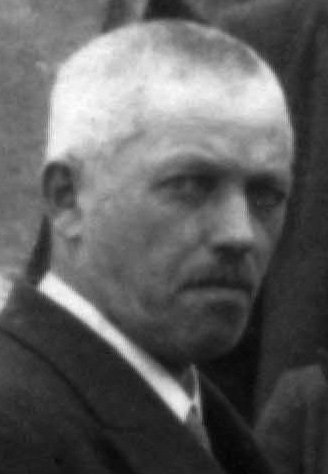
\includegraphics[width=3.836cm,height=5.556cm]{pictures/August-Hoegn_Nachruf.jpg}
 \par}
{\centering\bfseries
Band I: Hauptteil
\par}

{\centering
Zulassungsarbeit zur ersten Staatsprüfung für das Lehramt an Gymnasien,
\par}

{\centering
eingereicht bei Prof. Dr. Siegfried Mauser im Fach historische
Musikwissenschaft
\par}

{\centering
Ruhmannsfelden, München, April 2005
\par}

\clearpage{\bfseries
Inhaltsverzeichnis}

\subparagraph[Band I: Hauptteil]{Band I: Hauptteil}
\setcounter{tocdepth}{4}
\renewcommand\contentsname{}
\tableofcontents


\clearpage\setcounter{page}{1}\section{Vorwort}
\hypertarget{RefHeadingToc100333724}{}Als „Mozart von Ruhmannsfelden“
wurde August Högn in einer Ansprache an seinem 80. Geburtstag
bezeichnet. \footnote{Interview Nr. 24, Johann Glasschröder,
28.12.2004, Absatz 10} Der schmeichelnde Vergleich mit dem Salzburger
Komponisten war eine Verbeugung vor seinem jahrzehntelangen engagierten
Mitwirken am musikalischen Leben im kleinen Ort des Bayerischen Waldes
und besonders vor dem umfangreichen und in Ruhmannsfelden noch nie da
gewesenen kompositorischen Schaffen, auf das er zurückblicken konnte.
Auch ein beachtliches heimatkundliches Werk hatte er bis zu diesem
Zeitpunkt zusammengetragen und rechtfertige mehr als genug die weiteren
am letzten runden Geburtstag erteilten Ehren. Kaum größer könnte der
Unterschied zu Lebzeiten und heute sein, bezüglich der Würdigung seines
Schaffens und die Anerkennung seiner Dienste für die Allgemeinheit.
Fast 50 Jahre nach seinem Tod kennt kaum jemand der Ruhmannsfeldener
noch den Namen „August Högn“, geschweige denn sein musikalisches und
heimatkundliches Werk. Durch Zufall habe ich im Notenschrank der
Ruhmannsfeldener Pfarrkirche einige seiner Handschriften entdeckt, die
mein Interesse seinem Leben und Wirken erweckten und mich somit zu
Verfassen dieser Arbeit führten.

Ich möchte mit dieser Arbeit an das Leben und Werk des Rektors,
Heimatforschers und Komponisten August Högns erinnern, um somit seine
Person sowie Werk vor dem Vergessen zu bewahren. Da Högn sehr eng mit
meinem Heimatort Ruhmannsfelden verbunden war, wurde diese Arbeit fast
zwangsläufig zu einer „musikalischen Heimatkunde.“ Insofern kann man
die Arbeit auch als „Hommage an meine Heimat“ ansehen.

Bei der Erforschung von Högns Leben haben sich Berichte von Augenzeugen
als unverzichtbare Informationsquelle herausgestellt. Die Interviews
wurden mitgeschnitten (Daten-CD I) und transkribiert (Band II, Seite 7
- 56). Es war der letztmögliche Zeitpunkt durch Interviews mit
Zeitzeugen den hinter dem Werk stehenden Menschen aufzuzeigen. Der Tod
von zwei meiner meist hoch betagten Interviewpartner noch vor
Fertigstellung dieser Arbeit beweist eindringlich, wie schnell sich im
Laufe der Jahre die Spuren eines Menschen verwischen können, wenn sie
nicht rechtzeitig festgehalten werden.

Mehr als nur eine ergänzende Funktion zu den Interviews haben die in
eine Sammlung aufgenommen Dokumente. Ihnen ist es zu verdanken, dass
einige von Högns Lebensstationen, wie beispielsweise seine drei Phasen,
in denen er Chorregent war, zeitlich sehr genau bestimmt werden
konnten. Vor allem zum jungen Leben von Högn bildeten die Dokumente die
einzige Informationsquelle, da hier Augenzeugenberichte nicht mehr
möglich waren. Neben Dokumenten aus dem Gemeindearchiv waren besonders
die Archivalien, die das Pfarramt bereitstellen konnten, von
außerordentlichem Aufschlussreichtum in Bezug auf das Leben von August
Högn. Hier gab die „Chronik Ruhmannsfelden“ vom ehemaligen
Ruhmannsfeldener Pfarrer Franz Seraph Reicheneder nicht nur über Högns
Leben Auskunft, sondern auch über die Geschichte von Ruhmannsfelden.
Mancher Glücksfund erweitert zusätzlich das Spektrum an Schriftstücken,
zum Beispiel vier Briefe von Högn, die mir aus Australien übersandt
wurden. Sehr mühsam war die Entzifferung der in alter deutscher
Schreibschrift verfassten Dokumente. Einzige Möglichkeit, ihre Aussage
dauerhaft nachvollziehen zu können, blieb das Abschreiben. Da
handschriftliche Dokumente in der Sammlung überwiegen, habe ich mich
dazu entschlossen, alle Dokumente, auch die gut lesbaren, zu editieren.
So können alle Schriftstücke im Dokumentationsteil (Band II, Seite 57 -
90) wortwörtlich nachgelesen werden.

Der erste Teil dieser Arbeit handelt von Högns Leben. Eine Einbindung
und Bezugnahme von Högns musikalischem Werk in die Biographie war nicht
möglich, da man den Entstehungszeitpunkt der Kompositionen nur sehr
grob schätzen kann. Da sich sein Geschichtswerk hingegen sehr genau
zeitlich einordnen lässt und noch dazu viele Hintergrundinformationen
zur Entstehung bekannt sind, widmet sich ein Kapitel des ersten Teil
Högns heimatkundlichen Abhandlungen und ihrer Entstehung. Großer Wert
wurde auch auf die Abbildung der noch vorhandenen Fotos aus Högns
Privatleben gelegt, die große Aussagekraft leisten und den Text
auflockern.

Zum Erstellen des Werkverzeichnisses waren umfangreiche
Recherchearbeiten nötig. An mehreren unbekannten Plätzen lagerten Högns
Kompositionen, ehe sie ausfindig gemacht werden konnten. Die Anzahl der
Kompositionen steigerte sich im Laufe der Recherchearbeiten von den 12
Kompositionen aus dem Notenschrank in der Pfarrkirche Ruhmannsfelden,
dem ersten Fundort, auf fast 70 Werke. Um die tatsächliche Anzahl der
erhalten Werke festzustellen, musste der Kontakt zu Högns Nachfahren
hergestellt werden. Da alle Verbindungen zwischen der Ruhmannsfeldener
Bevölkerung sowie zwischen der Deggendorfer Verwandtschaft zu Högns
Enkelkindern abgerissen waren, gestaltete sich die Such nach den
Nachfahren entsprechend schwierig. Zwar besaßen die Nachfahren leider
auch keine Kompositionen mehr, doch konnte wenigstens die Suche als
beendet erklärt werden und das Werkverzeichnis bekam einen endgültigen
Charakter. Im Zuge der Durchsuchungsarbeiten nach Kompositionen am
Notenmaterial in der Pfarrkirche habe ich Listen aller Arrangements
(Seite \pageref{bkm:Ref100328080}) und aufgeführter Kompositionen (Band
II, Seite 99 - 101) von Högn angefertigt. Die Listen liefern eine
deutliche Abbildung von Högns musikalischem Umfeld und zeigen die
dadurch mögliche stilistische Beeinflussung auf Högns Werke auf. Einige
seiner Kompositionen wurden ediert (Band III) und lieferten den Anstoß
für etliche Wiederaufführungen (Band II, Seite 102 – 103, Daten-CD I).
Eine streng quellenbezogene Ausgabe der Werke mit kritischem Bericht
macht angesichts von Högns geringer Bedeutung in der Musikgeschichte
wenig Sinn. Stattdessen sollte das entstandene Notenmaterial mehr
aufführungspraktischen Überlegungen Rechnung tragen.

Der zweite Teil der Arbeit handelt vom musikalischen Werk Högns. Der
Beginn des Abschnitts „Werk“ ist vor allem um Rekonstruktion bemüht.
Fragen, die das Werkverzeichnis aufwirft, sollen hier beantwortet
werden. Abschließen wird auf einzelne Werke eingegangen. Da sich die
vorhergehenden Kapitel überwiegend mit der kirchenmusikalischen
Schaffen beschäftigt haben, wird dort auch auf seine weltliche
Kompositionen eingegangen. Neben seiner größten und wohl besten
geistlichen Komposition, der „Josephi“-Messe, erhalten auch die
weltlichen Kompositionen, nämlich der Marsch „In Treue fest!“ und der
Weihegesang Es-Dur ihren Platz. Högns einzig erhalte
nationalsozialistische Komposition soll bewusst nicht verschwiegen
werden. Ein Vergleich mit den geistlichen Grabliedern mag exemplarisch
darstellen, wie sich die damalige Propagandamusik Elemente aus anderen
Genres bediente.

Um Interessierten meine Forschungsergebnisse zugänglich zu mache, habe
ich eine Internetseite (www.august-hoegn.de) eingerichtet, die sich dem
Leben und Werk von August Högn widmet. Weitere noch zu verfolgende
Ziele wären eine Ausdehnung der regionalen Pflege seines musikalischen
Nachlasses von Ruhmannsfelden auf die Pfarreien das Dekanat Viechtach
und die Drucklegung einer heimatkundlichen Schrift über sein Leben und
Werk.

An dieser Stelle möchte ich mich bei den zahlreichen Personen bedanken,
die mir bei der Erforschung des Lebens und Werks von August Högn
behilflich waren. Ohne sie wäre diese Arbeit nicht möglich gewesen.
Eine Liste von über 40 am Projekt beteiligten Personen ist im Anhang
(Band II, Seite 104) zu finden.

München, April 2005\ \ \ \ \ \ \ \ Josef Friedrich

\section{Leben}

\subsection{Kindheit in
Deggendorf}


August Högn kam am 2. August 1878
in Deggendorf als Sohn von Andreas und Helene Högn, geborene Zöpfl, auf
die Welt. \footnote{Dokument Nr. 48, Zeitungsartikel aus Viechtacher
Bayerwald-Bote, 2.8.1958} August hatte zwei ältere Geschwister, Theres
(geboren 1869) und Ludwig (geboren 1871). Seine jüngeren Brüder, Joseph
und Otto, kamen 1879 und 1883 jeweils entsprechend auf die
Welt. \footnote{Grabinschrift der Familiengräber Andreas Högn und
Ludwig Högn am Deggendorfer Friedhof}

\begin{figure}
%
\begin{subfigure}[b]{0.5\linewidth}
\centering
\img[height=7cm]{Andreas-Hoegn}
\caption{Andreas Högn}
\end{subfigure}
%
\begin{subfigure}[b]{0.5\linewidth}
\centering
\img[height=7cm]{Helene-Hoegn}
\caption{Helene Högn}
\end{subfigure}
%
\caption{Die Eltern von August Högn}
\end{figure}

\begin{figure}
%
\begin{subfigure}[b]{0.5\linewidth}
\centering
\img[height=7cm]{Ludwig-Hoegn}
\caption{Ludwig Högn}
\end{subfigure}
%
\begin{subfigure}[b]{0.5\linewidth}
\centering
\img[height=7cm]{Joseph-Hoegn}
\caption{Joseph Högn}
\end{subfigure}
%
\caption{Zwei Brüder von August Högn}
\end{figure}

Augusts Vater war von Beruf Buchbinder und eröffnete zusammen mit seiner
Ehefrau 1867 eine Buchbinderei und Buchhandlung im so genannten
„Kerndel´schen-Haus“ am Luitpoldplatz in Deggendorf. Bereits nach 6
Jahren, also 1873, zog die Familie Högn in ein eigenes Haus in die
Pfleggasse 1, wo bis zum heutigen Tag die Buchhandlung Högn zu finden
ist (Abb. 5). Die äußerst günstige Lage der Buchhandlung im Zentrum
Deggendorfs war von bedeutendem wirtschaftlichen Vorteil. Besonders an
Markttagen, so zum Beispiel zum „Saumarkt“ in der Pfleggasse, strömten
viele Menschen aus der Umgebung nach Deggendorf, wovon auch die
Buchhandlung Högn profitierte. Das Sortiment wurde im Laufe der Zeit
erweitert und zusätzlich zu Büchern auch Schreib-, Schul-, Spiel- und
Lederwaren angeboten. Ab 1890 komplettierte ein eigener
Postkarten-Verlag das Angebot.\footnote{
http://www.hoegn.de/ueber/ueb\_gesch.php}

In dem Haus des späteren landgräflichen Magistratsrats, Landrats und
Landtagsabgeordneten \footnote{Grabinschrift des Familiengrabs Andreas
Högn am Deggendorfer Friedhof} Andreas Högn gehörte eine gründliche
Ausbildung und somit eine grundlegende musikalische Schulung der Kinder
allein schon zum guten Ton. Es ist daher kaum verwunderlich, dass alle
fünf Kinder das Klavierspielen erlernten, selbst der von Geburt an fast
taube Joseph Högn. \footnote{Interview Nr. 3, Ida Högn, 29.12.2002,
Absatz 40}

August Högn besuchte die Knabenschule in Deggendorf \footnote{Dokument
Nr. 48, Zeitungsartikel aus Viechtacher Bayerwald-Bote, 2.8.1958} und
war von 1889 bis 1891 Schüler der Unterstufe des Klosters Metten,
genannt Lateinschule, wo er auch im „Klosterseminar“, also im der
Schule angeschlossen Internat wohnte. \footnote{Korrespondenz Nr. 88,
Brief von P. Dr. Michael Kaufmann OSB an Josef Friedrich, 7.1.2005} Mit
dem darauffolgenden Übertritt in die Präparandenschule Deggendorf war
schon viel früher als bei anderen Schularten der endgültige Berufsweg
eingeschlagen. Die Übernahme des elterlichen Geschäfts dürfte für den
zweitgeborenen Sohn nie zur Debatte gestanden haben. Dies war
wahrscheinlich einer der Gründe, weshalb sich August frühzeitig für den
Beruf des Lehrers entschieden hatte. Ludwig Högn, der ältere Bruder von
August, erlernte ganz nach alter Tradition das Buchbinderhandwerk, um
einmal die Stellung seines Vaters einnehmen zu können. Er eröffnete
jedoch in Straubing eine Kunst-, Papier- und Galanteriewarenhandlung.
Somit konnte der jüngste Sohn Otto die Buchhandlung Högn
übernehmen. \footnote{Interview Nr. 26, Eva Ertl, 9.2.2005, Absatz 2}

\begin{figure}
\img{Buchhandlung-Hoegn_2004}
\caption{Buchhandlung Högn, 2004}
\end{figure}

\subsection{Musikalische Lehrerausbildung}

\hypertarget{RefHeadingToc100333727}{}Die Entscheidung, eine Ausbildung
zum Volksschullehrer anzutreten, wurde für August Högn sicher auch
dadurch erleichtert, dass sich in der Deggendorfer Arachauergasse Nr.
94 (heutige Bräugasse Nr. 14) wenige Minuten Fußmarsch entfernt von
Augusts Elternhaus eine Präparandenschule (Abb. 6) befand. Wie zu
Volksschul-Zeiten konnte er wieder bei seinen Eltern wohnen und war
nicht mehr auf das Mettener Internat angewiesen. \footnote{Goller,
Seite 24}

Die damalige Lehrerausbildung dauerte fünf Jahre. An eine dreijährige
Vorbereitungsphase an einer Präparandenschule schloss sich die
eigentliche zweijährige Ausbildung in der Lehrerbildungsanstalt
Straubing an. Neben der Bezeichnung „Präparandenschule“, die so viel
bedeutet wie „Schule der Vorzubereitenden“, ist aus heutiger Sicht vor
allem ungewöhnlich, dass es damals gleich zwei verschiedene Schularten
gab, die vom angehenden Lehrer durchlaufen werden mussten, nämlich die
dreijährige Vorbereitungsphase an einer Präparandenschule und die
zweijährige Ausbildung in der Lehrerbildungsanstalt. Diese Tatsache
lässt sich aus der historischen Entwicklung der Lehrerausbildung
erklären. Es war Jahrhunderte lang Praxis, dass Handwerker zusätzlich
zu ihrer beruflichen Tätigkeit auch die Unterweisung der Schulkinder in
den Grundfertigkeiten wie Lesen, Schreiben und Rechen übernahmen. Die
Verordnung vom 4. September 1823 schrieb erstmals verpflichtend eine
zweijährige Ausbildung für angehende Lehrer vor und hob so
gewissermaßen den Berufsstand des Volkschullehrers im Königreich Bayern
aus der Traufe. Zuvor sollten die Anwärter drei Jahre lang bei einem
\zitat{„tüchtigen Schullehrer“ } \footnote{Lippert, Seite
153} oder einen \zitat{„vorzüglichen Geistlichen“ }\footnote{
Lippert, Seite 153} eine Art Lehre oder Praktikum ablegen, ehe man sie
ins Lehrerseminar aufnahm. Da sich diese Art der Vorbildung als nicht
effektiv herausgestellt hatte, wurde mit dem Normativ vom 29. September
1866 die dreijährige Vorbereitungszeit durch Einführung der
Präparandenschulen straffer organisiert. \footnote{Lippert, Seite 154}

Ebenso ungewöhnlich aus heutiger Sicht und kaum mit der Ausbildung der
Grund- und Hauptschullehrer vergleichbar ist die starke Gewichtung des
Musikunterrichts in der gesamten damaligen Volksschullehrerausbildung,
besonders aber in den Anfangsjahren der Präparandenschule. Das Fach
Musik – es ließ sich in die Teilbereiche \zitat{Gesang,
Violine, Klavier, Orgel }und\zitat{ Harmonielehre
}unterteilen – hatte innerhalb des Fächerkanons einen so hohen
Stellenwert, dass es neben Religionslehre, Deutsch und Rechnen
ebenfalls als Hauptfach bezeichnet wurde. \footnote{Lippert, Seite 165}
Mit 6 Wochenstunden machte der Musikunterricht mehr als ein Fünftel an
der Gesamtstundenzahl aus und zeigt deutlich die Ausrichtung der
Ausbildung, die angehenden Lehrer auf den Chorregenten- und
Organistendienst vorzubereiten. \footnote{Goller, Seite 11} Wie alle
Fächer, so wurde auch der Instrumentalunterricht von Volksschullehrern
erteilt, die an die Präparandenschule berufen worden waren.\footnote{
Goller, Seite 33} Da die Schüler vor Eintritt in die Präparandenschule
keine Vorkenntnisse im Spiel der Musikinstrumente mitbringen brauchten,
kam es oft vor, dass im Instrumentalunterricht bei einer Gruppenstärke
von durchschnittlich 10 Schülern unter den einzelnen Schülern sehr
große Leistungsunterschiede herrschten. So musste sich beispielsweise
ein fortgeschrittener Schüler, wie es August Högn im Klavierspiel war,
zusammen mit Anfängern eine Stunde teilen. Beim Klavierunterricht stand
die Hinführung auf das Orgelspiel im Vordergrund und somit die Pflege
des \zitat{„gebundenen Spiels.“}  \footnote{Goller, Seite 38}
Die Schüler sollten in der dreijährigen Ausbildung die Fähigkeit
entwickeln, leichte Sonaten und Sonatien von Bertini, Czerny, Clementi,
Dussek, und Kuhlau zu spielen. Der Orgelunterricht begann ab dem II.
Kurs, also dem 2. Schuljahr, nach Barners Schule „Anfänge des
Pedalspiels“ und bediente sich im III. Kurs der Orgelschule von
Herzog. \footnote{Goller, Seite 39} Praktische Kirchenmusikerfahrung
konnten die Schüler als Choristen unter der Woche bei der Gestaltung
von Schulmessen und an Feiertagen bei Gottesdiensten an der königlichen
Kreisirrenanstalt mit Messkompositionen der Cäcilianer Witt, Zangl,
Haberl und Ett sammeln. Sowohl die Lehrer als auch die Schüler waren
Mitglieder des Bezirk-Cäcilien-Vereins Metten und des
Pfarr-Cäcilien-Vereins Deggendorf. \footnote{Goller, Seite 47}

\begin{figure}
\centering
\img[width=5cm]{Praeparandenschule}
\caption{Gebäude der ehemaligen Präparandenschule in der heutigen
Bräugasse Nr. 14 in Deggendorf}
\end{figure}

\begin{figure}
\img{Lehrerbildungsanstalt}
\caption{Lehrerbildungsanstalt in Straubing (Ansicht gegen die
Pfarrkirche St. Jakob)}
\end{figure}

So eng die Präparandenschule und die Lehrerbildungsanstalt inhaltlich
ineinander griffen, so unterschiedlich dürfte August Högn die beiden
Schulen erlebt haben, bezüglich der Gewährung von persönlichem
Freiraum. Der seit Bestehen der Lehrerbildungsanstalt geltende
Internatszwang verliehen dem Seminar in Straubing den Charakter einer
geschlossenen Anstalt. Ein von 5 bis 21 Uhr genau festgelegter
Tagesablauf forderte von den Schülern große
Anpassungsleistungen. \footnote{Goller, Seite 61} Selbst Spaziergänge
fanden nicht ohne Aufsicht statt. Man legte großen Wert auf das
Erlernen der Fähigkeit, sich unterzuordnen, auch wenn dies nicht
explizit im Lehrplan aufgeführt war. Das hat wohl die Eingliederung der
Lehrer in die Gesellschaft an der Wende zwischen dem 19. und 20.
Jahrhundert gefördert sowie die Übernahme der Aufgaben und Pflichten,
die von dieser Gesellschaft an die Lehrer herangetragen wurden. Die
Unterordnung begünstigte aber auch wahrscheinlich die so genannte
„Untertanenmentalität“, die als ein Grund unter vielen genannt wird,
weshalb es zur Machtergreifung der Nationalsozialisten und ihrer
schrecklichen Verbrechen an der Menschlichkeit gekommen war. Wie
bereits viele Lehrer, ließ sich auch August Högn in die von den
Nationalsozialisten entworfene Gesellschaftsordnung bruchlos einordnen
und zur Übernahme von Aufgaben bewegen, die ihrerseits die Herrschaft
der Nazis unterstützten.

Während die Stundenanzahl und die Fächerverteilung im Fach Musik in etwa
mit dem Lehrplan der Präparandenschule zu vergleichen war,
unterrichteten in Straubinger Seminar nicht ehemalige Volksschullehrer
mit normaler Lehrerausbildung, sondern speziell ausgebildete Musiker.
Anton Schwarz prägte von 1892 bis 1923 das musikalische Leben an der
Lehrerbildungsanstalt maßgeblich. \footnote{Stengl, Seite 104} Er hatte
nach zwölfjährigem Volksschuldienst beim Joseph Rheinberger Komposition
und Orgel an der königlichen Musikschule in München studiert und konnte
sein erworbenes Wissen in den Fächern Harmonielehre, Orgel und Gesang
an die Schüler weitergeben. \footnote{Goller, Seite 92} Sein
umfangreiches kompositorisches Schaffen, darunter vier Messen, mehrere
Offertorien und Motetten, lieferte für manche Schüler einen Ansporn,
sich selbst im Komponieren zu versuchen. \footnote{Goller, Seite 93}

\begin{center}
\begin{minipage}{4.269cm}
\begin{flushleft}
\tablefirsthead{}
\tablehead{}
\tabletail{}
\tablelasttail{}
\begin{supertabular}{m{4.0690002cm}}

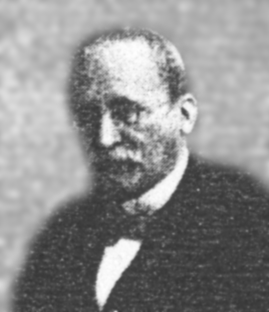
\includegraphics[width=3.886cm,height=4.531cm]{pictures/zulassungsarbeit-img010.png}

Anton Schwarz\\
\end{supertabular}
\end{flushleft}
\end{minipage}
\end{center}
{\centering

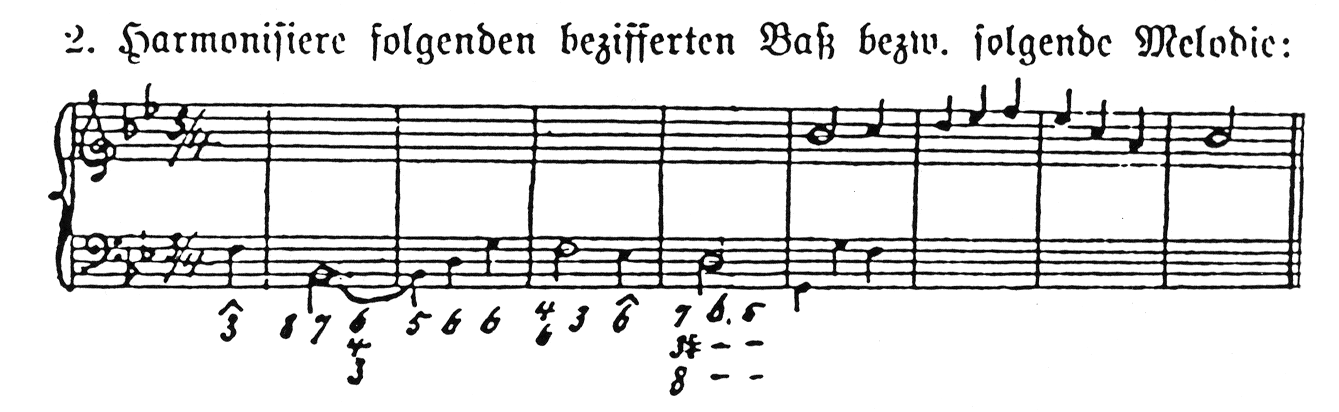
\includegraphics[width=11.088cm,height=3.258cm]{pictures/zulassungsarbeit-img011.png}
 \par}
{\centering
\label{bkm:Ref100298600}Schlussprüfung
der niederbayerischen Präparandenschulen 1903
\par}

Die Schüler erhielten zwar in ihrer Ausbildung zum Lehrer keinen
Kompositionsunterricht, dafür vermittelte ihnen der
Harmonielehreunterricht die wichtigsten tonsätzerischen Regeln, mit
denen sie in Eigenregie erste kompositorische Schritte wagen konnten.
Wie die im Fach Harmonielehre gestellten Prüfungen zeigen (Abb. 9),
gehörte das Umgehen mit dem vierstimmigen Chorsatz zu dem Handwerkszeug
eines angehenden Lehrers. Man kann deshalb August Högns Werke – sie
haben mit wenigen Ausnahmen den vierstimmigen Satz als Grundgerüst –
als Früchte des Musikunterrichts der Lehrerausbildung
betrachten. \footnote{Goller, Seite 74}

\subsection{Wanderjahre}

\hypertarget{RefHeadingToc100333728}{}Nach seinem Abschluss, dem
sogenannten „Absolutorium“, an der Lehrerbildungsanstalt in Straubing
1898, absolvierte August Högn an seiner ehemaligen Knabenschule in
Deggendorf ein Praktikum bei den Lehrern Buchner und Edelmann. Als
Aushilfslehrer waren seine Stationen Neukirchen bei Haggn im Landkreis
Straubing-Bogen, Schaufling bei Deggendorf und Geratskirchen in der
Nähe von Eggenfelden. Im Rang eines Hilfslehrers unterrichtete er in
Zeilarn bei Simbach am Inn und Wallersdorf. 1902 legte er an der
Regierung von Niederbayern die Anstellungsprüfung ab und wurde ab 1.
Januar 1903 Schulverweser in Wallersdorf. \footnote{Dokument Nr. 48,
Zeitungsartikel aus Viechtacher Bayerwald-Bote, 2.8.1958}
„Schulverweser“ ist eine 1896 eingeführte Bezeichnung für den
Schulgehilfen, also den zweiten Lehrer und Vertreter des
Schulleiters.\footnote{
http://www.markt-pfaffenhofen.de/geschichte/html\_geschichte/die\_schulverweser\_in\_pfaffenhofen.htm}
Dort lernte er seine Ehefrau Emma kennen.

\begin{figure}
\img{August-Hoegn_Wanderjahre}
\caption{August Högn}
\end{figure}

\begin{figure}
\img{Emma-Hoegn}
\caption{Emma Högn}
\end{figure}

\begin{figure}
\img{Hochzeitseinladung-und-Menue}
\caption{Hochzeitseinladung und Menü}
\end{figure}

Am 20. Juli 1904 fand in Wallersdorf die Hochzeit von August Högn und
der neun Jahre jüngern, damals 16-jährigen Emma Gerstl mit üppigem
Hochzeitsmenü statt, wie der Hochzeitseinladung (Abb. 12) entnommen
werden kann. \footnote{Dokument Nr. 111, Einladung zur Hochzeitsfeier,
20.7.1904} Emma Gerstl stammte aus einer wohlhabenden\footnote{
Interview Nr. 4, Maria Schröck, 30.12.2002, Absatz 4}
Bierbrauerfamilie,die in Gründobl, einem
kleinen Ort in der Nähe von Wallersdorf, ein großes Anwesen mit
Brauerei \footnote{Interview Nr. 21, Lilo Leuze, 2.12.2004, Absatz 20}
und Wirtshaus \footnote{Interview Nr. 3, Ida Högn, 29.12.2002, Absatz
36} besaß. Das junge Paar musste heiraten, da Emma Högn schwanger
wurde. Sie gebar Zwillinge, die beide kurz nach ihrer Geburt
starben. \footnote{Interview Nr. 3, Ida Högn, 29.12.2002, Absatz 36;
Interview Nr. 25, Lilo Leuze, 14.1.2005, Absatz 2} Zum 1. Juni 1905
wurde Högn nach Eberhardsreuth im Landkreis Grafenau
versetzt. \footnote{Dokument Nr. 48, Zeitungsartikel aus Viechtacher
Bayerwald-Bote, 2.8.1958} Hier kam die Tochter Elfriede, genannte
Frieda, am 14. August 1906 zur Welt. \footnote{Interview Nr. 20,
Gertraud von Molo, 23.11.2004, Absatz 6} Der Sohn Gustl erblickte am
17.1.1912 schon in Högns nächstem Einsatzort das Licht der Welt: in
Ruhmannsfelden. \footnote{Taufregister der Pfarrgemeinde St.
Laurentius, Ruhmannsfelden}

\begin{figure}
\img{Gustl-und-Frieda-Hoegn}
\caption{Gustl und Frieda Högn}
\end{figure}

\subsection{Schnelle Integration in Ruhmannsfelden}

August Högn wurde zum 1.1.1910 an
die Volksschule in Ruhmannsfelden versetzt. \footnote{Dokument Nr. 48,
Zeitungsartikel aus Viechtacher Bayerwald-Bote, 2.8.1958} Der Markt
Ruhmannsfelden, in dem damals ungefähr 1500 Einwohner lebten, liegt im
bayerischen Wald und ist etwa in der Mitte des Dreiecks zu finden, das
die nächst gelegenen drei Städte Viechtach, Regen und Deggendorf
bilden. \footnote{Högn, Ruhmannsfelden, S. 50} Das Einzugsgebiet der
Volksschule umfasste auch vor dem 1. Weltkrieg nicht nur die Gemeinde
Ruhmannsfelden, sondern zusätzlich weite Teile der benachbarten
Gemeinde Zachenberg und Randgebiete der angrenzenden Gemeinde
Patersdorf, also in etwa das Gebiet der Pfarrei St. Laurentius. Die
Gemeinde Zachenberg, die geringfügig mehr Einwohner als Ruhmannsfelden
zählte, bestand aus 38 überwiegend landwirtschaftlich geprägten
Kleinstortschaften und hatte mit dem Dorf Zachenberg kein wirkliches
Zentrum, denn dort bestand weder ein Rathaus noch ein Schulhaus. Nicht
nur in Schulangelegenheiten war Ruhmannsfelden damals wie auch heute
ein Zentrum. Ansässige Ärzte und eine seit 1910 bestehende
Apotheke \footnote{Högn, Ruhmannsfelden, S. 28 – 29} lieferten auch für
die Bewohner der Nachbargemeinden Achslach und Gotteszell einen Grund,
Ruhmannsfelden zu besuchen.

\begin{figure}
\img{Ruhmannsfelden}
\caption{Ruhmannsfelden zur Zeit August Högns}
\end{figure}

Man kann davon ausgehen, dass Högn Ruhmannsfelden als einen
fortschrittlichen Ort erlebt hat, da dort kurz vor seiner Ankunft
Investitionen getätigt und Reformen durchgeführt wurden. So besaß
Ruhmannsfelden seit dem Schulhausneubau im Jahr 1908 (Abb. 16) gleich
drei Schulhäuser. \footnote{Reicheneder-Chronik, Schulwesen, Blatt 76
Vorderseite} Das älteste, 1834 erbaute Schulhaus (Abb. 15) konnte als
Lehrerwohnhaus genutzt werden und bot somit der jungen Familie eine
Wohnmöglichkeit. \footnote{Reicheneder-Chronik, Schulwesen, Blatt 68
Vorderseite} Auch in institutioneller Hinsicht hatte sich an der
Volksschule Ruhmannsfelden kurz vor 1910 Einiges geändert. Dem
Anwachsen der Schülerzahl wurde Rechnung getragen und statt früher vier
unterrichten nun sieben Lehrer, also ein Lehrer pro Schülerjahrgang.
Den jahrgangsübergreifenden und nach Geschlechtern getrennten Klassen
war somit ein Ende gesetzt. Die gemischten Jahrgänge umfassten aber
immer noch fast durchschnittlich 70 Schüler.\footnote{
Reicheneder-Chronik, Schulwesen, Blatt 16 Rückseite} 1908 hatten die
Anträge der Gemeinden Zachenberg und Patersdorf auf Einführung einer
Sommerschule Erfolg. Damit Kinder vor allem zur Erntezeit in der
Landwirtschaft ihrer Eltern mithelfen konnten, wurde vom 1. Mai bis 1.
Oktober ein auf drei Stunden verkürzter Unterricht
eingeführt. \footnote{Reicheneder-Chronik, Schulwesen, Blatt 8
Vorderseite}

\begin{figure}
%
\begin{subfigure}[t]{0.3\linewidth}
\centering
\img[height=3cm]{Schulhaus-1834}
\caption{Schulhaus von 1834, ab 1908 als Lehrerwohnhaus genutzt}
\end{subfigure}
%
\begin{subfigure}[t]{0.7\linewidth}
\centering
\hfil\img[height=3cm]{Schulhaus-1908}
\caption{Schulhaus von 1908}
\end{subfigure}
%
\caption{Die Ruhmannsfeldener Schulhäuser}
\end{figure}

Mit August Högn traten gleich drei neue Lehrer in Ruhmannsfelden ihren
Schuldienst an. In der Schulchronik wird Högn bald als 2. Lehrer und
somit Stellvertreter von Schulleiter Alois Auer aufgeführt.\footnote{
Volksschul-Chronik} Das hatte neben seiner schon 10 Jahre langen
Berufserfahrung wahrscheinlich auch den Grund, dass Högn die einzige
männliche Lehrerkraft neben Bezirksoberlehrer Auer war, die in den
unruhigen Zeiten des 1. Weltkrieges seiner neuen Heimat treu bleiben
konnte. Högns Kriegseinsatz beschränkte sich auf einen kurzen
Heeresdienst im Jahr 1915, bei dem er sich den König-Ludwig-Orden und
das Militär-Verdienstkreuz erwarb.

Eine weitere Neuerung war, dass die Pfarrkirche St. Laurentius im selben
Jahr, als August Högn nach Ruhmannsfelden kam, eine neue, pneumatische
Orgel mit 22 Registern vom Orgelbaumeister Ludwig Edenhofer aus
Deggendorf bekam. \footnote{Reicheneder-Chronik, Orgel, Blatt 74
Rückseite} Von Anfang an wirkte Högn an der Kirchenmusik in
Ruhmannsfelden mit. \footnote{Dokument Nr. 18, Brief von August Högn an
Pfarrer Reicheneder, 25.1.1954} Der versierte Orgelspieler\footnote{
Interview Nr. 16, Maria Freisinger, 25.8.2004, Absatz 28} war auch im
Kirchendienst mehr als ein würdiger Stellvertreter für Auer, der
zusammen mit seiner Frau Anna und Tochter Auguste den
Chorregentendienst ausführte.

Bereits ein halbes Jahr nach seiner Ankunft wurde Högn zum Vorstand
eines Ruhmannsfeldener Vereins gewählt, was seine schnelle
gesellschaftliche Integration in Ruhmannsfelden unterstreicht. Der
Turnverein Ruhmannsfelden suchte zu dem Zeitpunkt händeringend eine
Person, die sich bereit erklärte, den unbesetzten Posten des Vorstands
zu übernehmen. Vom 21.5.1910 \footnote{Dokument Nr. 101, Protokoll der
Turnvereinsversammlung, 21.5.1910}  bis 27.12.1913 \footnote{Dokument
Nr. 103, Protokoll der Turnvereinsversammlung, 27.12.1913} hatte Högn
dieses Amt inne. Auch wenn er nach dieser Zeit in keiner Funktion der
Vereinsspitze in Erscheinung tritt, blieb er trotzdem über Jahrzehnte
hinweg vor allem als Leiter der Sänger- und Orchesterriege dem Verein
treu. 1924 versuchte man noch einmal Högn in die Vereinsspitze als
Schriftführer mit einzubinden, doch er lehnte wahrscheinlich deswegen
ab, weil er schon bei der Ruhmannsfeldener Feuerwehr die
Schriftführertätigkeit ausübte. \footnote{Dokument Nr. 107, Protokoll
der Turnvereinsversammlung, 23.1.1924}

August Högn war bereits am 19.9.1902 der Wallersdorfer Feuerwehr
beigetreten \footnote{Dokument Nr. 110, Abschiedsrede des
Feuerwehrkommandanten Johann Linsmeier auf August Högn, 3.11.1951} und
wechselte Anfang Januar 1910 in die Feuerwehr Ruhmannsfelden. Am
26.12.1910 wurde Högn dann zum Schriftführer der Feuerwehr
Ruhmannsfelden gewählt. \footnote{Dokument Nr. 93, Protokoll der
Feuerwehrgeneralversammlung, 26.12.1910} Dass ein Lehrer den
Schriftführerposten der Feuerwehr übernahm, hatte in Ruhmannsfelden
Tradition. Die Lehrer Raymund Schinagl und Max Weig waren lange Zeit
vor Högn als Schriftführer tätig. Der Feuerwehr-Mitbegründer und letzte
Schriftführer Joseph Lukas starb am 30.8.1910, \footnote{Högn,
Feuerwehr, Blatt 7 b, Blatt 17, Blatt 34} sodass sein Posten frei
wurde. August Högn, als Lehrer im Schreiben souverän wie sonst kein
anderer bei der Feuerwehr, bot sich als Nachfolger für Lukas gerade zu
an. Die Protokolle vor Högns Zeit als Schriftführer zeichnen sich
dementsprechend durch viele Rechtschreibfehler aus.\footnote{
Feuerwehr-Protokoll} August Högn blieb 40 Jahre lang Schriftführer der
Feuerwehr. Neben dem Verfassen von Protokollen übernahm er die
Korrespondenz der Feuerwehr, hielt zahlreiche Ansprachen und Vorträge
und packte auch mal mit eigenen Händen an, als zum Beispiel 1933 bei
strömenden Regen die neue Feuerwehrspritze vom Zug abgeladen werden
musste. \footnote{Högn, Feuerwehr, Blatt 44, Blatt 46, Blatt 47, Blatt
54, Blatt 56}

Ein weiteres Aufgabenfeld, das die damalige dörfliche Gemeinschaft für
einen Lehrer bereithielt, übernahm August Högn 1913: Bis 1920 war August
Högn Gemeindeschreiber der Gemeinde Zachenberg. \footnote{Högn,
Zachenberg, Blatt 16} Nach dem Erlass der Gemeindeverordnung wurden
diese Arbeiten hauptsächlich den Lehrern übertragen. \footnote{Geyer,
Seite 106} So verwundert es nicht, dass die angehenden Lehrer in den
Lehrerbildungsanstalten speziell im Fach Gemeindeschreiberei
unterrichtet wurden \footnote{Dantl, Seite 82} und dass vor Högn die
Lehrer Milter, Schinagl, Lechner und Hochstraßer für die Gemeinde
Zachenberg tätig waren. \footnote{Högn, Zachenberg, Blatt 11, Blatt 15,
Blatt 16} Högns Eifer, sich für das Gemeinwohl zu engagieren, kommt auch
dadurch besonders zum Ausdruck, dass er sogar ein Zimmer seiner
Dienstwohnung abtrat und es in eine Art Gemeindekanzlei umwandelte.
Vorher wurden die Gemeindearbeiten, die für Lehrer eine wichtige
Nebeneinkunft darstellten, in einem Raum der Brauerei Rankl in
Ruhmannsfelden erledigt.

\subsection{Leiter des Turnverein-Orchesters}

Ähnlich wie andere Vereine am Ort, veranstaltete der Turnverein
Ruhmannsfelden bunte Abende oder führte Theaterstücke, Singspiele und
sogar Operetten auf und übernahm somit weit über die eigentliche
Vereinsaufgabe hinaus eine wichtige kulturelle Funktion.
\footnote{Dokument Nr. 56, Auszug aus den Memoiren von Franz Danziger
sen., 1984} Zumindest für den Turnverein war die Veranstaltung
derartiger Unterhaltungsprogramme eine bedeutende Einnahmequelle für die
Finanzierung geplanter Projekte wie beispielsweise den Turnhallenbau. Es
ist daher keineswegs verwunderlich, dass sich für August Högn in den
Anfangsjahren in Ruhmannsfelden insbesondere unter dem Dach des
Turnvereins ein musikalisches Betätigungsfeld auftat, obwohl die
ursprüngliche Aufgabe des Vereins nichts mit Musik zu tun hatte. Der
ehemalige Vorstand unterstützte den Verein nun als Leiter einer Sänger-
und Orchesterriege. \footnote{Dokument Nr. 98, Geschichtliches über die
Erbauung der Turnhalle in Ruhmannsfelden, 1928}

Am 27.9.1919 wurde die Sängerriege im Turnverein gegründet. Als erster
Leiter erscheint zwar Rudolf Schwannberger, Nachbar von Högn und
Kirchenchorsänger. \footnote{Dokument Nr. 104, Protokoll der
Turnvereinsversammlung, 27.9.1919} Doch laut des Turnverein-Protokolls
fungierte Högn bereits ab 29.12.1919 als Dirigent. \footnote{Dokument
Nr. 105, Protokoll der Turnvereinsversammlung, 29.12.1919} 1921 wird
Schwannberger als Gesangswart und Högn als Gesangsdirigent der
Sängerriege bezeichnet, \footnote{Dokument Nr. 106, Protokoll der
Turnvereinsversammlung, 10.12.1921} die sich im Saal der Brauerei
Vornehm zum Proben traf. Über die Orchesterriege, die im Haus des
Apothekers Voit probte, sind im Vereinsprotokoll keine Eintragungen zu
finden. Wahrscheinlich kam das Streichorchester nur dann zusammen, wenn
ein Stück eine Instrumentalbegleitung der Sänger benötigte.

\begin{figure}
%
\begin{subfigure}[t]{0.5\linewidth}
\centering
\img[height=7cm]{Rudolf-Schwannberger}
\caption{Rudolf Schwannberger}
\end{subfigure}
%
\begin{subfigure}[t]{0.5\linewidth}
\centering
\img[height=7cm]{August-Hoegn_Turnverein}
\caption{August Högn}
\end{subfigure}
%
\caption{Der Gesangswart und der Gesangsdirigent der Sängerriege}
\end{figure}

Leider ist nur wenig über die Veranstaltungen im Einzelnen bekannt. Es
ist nicht bekannt, wie regelmäßig sie stattfanden und in welchem
Zeitraum der Turnverein sich derart kulturell engagierte. Einen kleinen
Einblick in das damalige kulturelle Leben gewährt uns aber, die nicht
nur in finanzieller Hinsicht erfolgreichste „Produktion“ des
Turnvereins: die Aufführungen des Singspiels „Der Holledauer Fidel“ von
Erhard Kutschenreuter im Jahr 1923. \footnote{Dokument Nr. 98,
Geschichtliches über die Erbauung der Turnhalle in Ruhmannsfelden,
1928} Dieses Singspiel forderte eine große Anzahl an Mitwirkenden. Im
dritten Akt ist beispielsweise ein Trachtenfestzug verlangt, der über
die Bühne zieht. \footnote{Proft, Seite 58} Große Anforderungen an die
Gesangeskünste der Mitwirkenden stellten die vielen Gesangsnummer des
Singspiels, wie etwa das Liebeslied des Fidel, das Duett des Sichbauern
und dessen Frau, das Lied der Reserl, ein Kinderchor und die großen
Chorszenen zu Beginn und zum Schluss des Singspiels. \footnote{Proft,
Seite 57} Instrumentalstücke, wie zum Beispiel das polyphon angelegt
Vorspiel zum zweiten Akt \footnote{Proft, Seite 55} der
„Holledauer-Marsch“ und der „Waldler-Marsch“, \footnote{Proft, Seite
57} stellten eine Herausforderung für das Turnverein-Orchester dar, das
aus drei Violinen und einer Viola, einem Violoncello und einem
Kontrabass, also sechs Musikern, ähnlich wie das Kirchenorchester,
bestand.

\begin{figure}
\img{Holledauer-Fidel}
\caption{Die Mitwirkenden der Aufführungen des Singsspiels „Der
Holledauer Fidel“}
\end{figure}

Die ca. 60 an den 8 Aufführungen des Singsspiels „Der Holledauer Fidel“
von Erhard Kutschenreuter im März 1923 beteiligten Personen. In der
Mitte (Pfeile) sind August Högn und seine Tochter Frieda zu sehen.

Diese ungewöhnlich große Anzahl an Mitwirkenden – auf dem Foto (Abb. 19)
sind 60 Personen zu sehen – machte es notwendig, dass die Bühne im
Vornehmsaal ausnahmsweise an der Längsseite aufgestellt werden musste,
sodass die Akteure nur direkt vom Freien aus auf die Bühne gelangen
konnten. \footnote{Dokument Nr. 98, Geschichtliches über die Erbauung
der Turnhalle in Ruhmannsfelden, 1928} Die große Teilnehmerzahl ist auf
die Unterstützung weiterer Vereine zurückzuführen, insbesondere jedoch
des Kirchenchores und der Lehrerschaft. August Högn, der die gesamte
musikalische Leitung übernommen hatte und als Dirigent fungierte, war
in seiner Eigenschaft als Chorregent und Schulleiter der ideale Mann,
weitere geeignete Mitwirkende für das Singspiel zu gewinnen.

Die Einkünfte der acht im Saal der Brauerei Vornehm stattgefundenen und
ausverkauften Aufführungen des Singspiels erbrachten einen Gewinn von
500 M, mit dem ein Grundstück erworben werden konnte, das als Turnplatz
verwendet wurde. \footnote{Dokument Nr. 95, Programmzettel zur
Aufführung des Singspiels {\textquotedbl}Der Holledauer
Fidel{\textquotedbl}, Mrz. 1923} Dieser durchschlagende Erfolg der
Aufführungen des „Fidels“ – sie verhalfen dem Turnverein sogar zu einem
eigenen Turnplatz – ist auch auf das Stück zurückzuführen. Mit dem
„Fidel“ hatte der im Rottal ansässige Lehrer Erhard Kutschenreuter mit
Abstand sein erfolgreichstes Stück geschrieben. \footnote{Proft, Seite
53} Nach der Uraufführung in Passau im Jahr 1920 erlebte das Singspiel
schon 1938 die 3000. Aufführung. \footnote{Proft, Seite 60} Die
Ruhmannsfeldener Zuschauer strömten vielleicht auch deswegen so
zahlreich in die Vorstellungen weil die Handlung des Stückes zum Teil
im bayerischen Wald spielt: Der arme Hopfenzupfer Fidel Waldhauser aus
dem bayerischen Wald verliebt sich in die Tochter des reichen
Sichbauern aus der Hallertau, gespielt von August Högns Tochter
Frieda. \footnote{Dokument Nr. 95, Programmzettel zur Aufführung des
Singspiels {\textquotedbl}Der Holledauer Fidel{\textquotedbl}, Mrz.
1923} Trotz auftretender Hindernisse, die unüberwindbar zu sein
scheinen, findet das ungleiche Paar schließlich doch zusammen, und es
kommt zur Hochzeit. Den Zuschauern in Ruhmannsfelden waren die
dargestellten sozialen Verhältnisse sicher gut bekannt, denn viele von
ihnen fuhren selbst, wie es bis in den fünfziger Jahren des letzten
Jahrhundert üblich war, einmal jährlich in die Hallertau zur
Hopfenernte, um ein Zusatzeinkommen zu verdienen. \footnote{Proft,
Seite 56}

\begin{figure}
\img{Programm_Holledauer-Fidel}
\caption{Programm zu den „Fidel“-Aufführungen}
\end{figure}

Am 21. Juli 1923 wurde August Högn von der Gemeinde Ruhmannsfelden das
Ehrenbürgerrecht \zitat{„aus Anlass seines 25-jährigen Dienstjubiläums“}
\footnote{Reicheneder-Chronik, Ehrenbürger, Blatt 1 Vorderseite} und
\zitat{„für die großen Verdienste, die er sich um Schule und Gemeinde
erwarb“} \footnote{Reicheneder-Chronik, Ehrenbürger, Blatt 1
Vorderseite} verliehen. Dieser Titel stellte damals schon eine besondere
Auszeichnung dar und wurde daher nur an wenige sich außerordentlich
verdient gemachte Bürger verliehen. Die Ehrenbürgerurkunde bekamen
außerdem Pfarrer Mühlbauer (1906) sowie August Högns Vorgänger als
Schulleiter Alois Auer (1910). Nach Högn wurde sie 1933 an Adolf Hitler
verliehen. \footnote{Reicheneder-Chronik, Ehrenbürger, Blatt 1
Vorderseite} Die Aufführungen des „Holledauer Fidels“ etwas länger als
ein Vierteljahr davor, lassen den Anlass für die Ehrenbürgerrechts-
Verleihung Högns in ganz anderem Licht erscheinen. Ist es nicht
offensichtlich, dass die Singspielabende, an denen Högn in
hervorragender Weise mitgearbeitet hatte und die dem Turnverein zum
Erwerb eines Turnplatzes verhalfen, eher als der Hauptgrund für die
Verleihung anzusehen ist, als sein 25. Dienstjubiläum, das wohl eher
einen weiterem Grund darstellt?

Aus finanzieller Sicht war der Turnverein am Bau seiner eigenen
Turnhalle mit einem großen Betrag beteiligt. Die Einkünfte vieler
bunter Abende sowie weitere Theateraufführungen, wie z. B. die
Aufführung der Operette „Der Postillion“  \footnote{Dokument Nr. 56,
Auszug aus den Memoiren von Franz Danziger sen., 1984} von Ludwig
Eckl, \footnote{Goller, Seite 188} dürften direkt in den Turnhallenbau
geflossen sein. Högn engagierte sich nicht nur musikalisch für die
Anliegen des Turnvereins, sondern auch politisch. 1925 begrüßte er eine
Kommission des bayerischen Landtages in Ruhmannsfelden und äußerte
ihnen unter anderem die Bitte um Bezuschussung des Turnhallenbaus. Am
29. Januar 1928 wurde die Ruhmannsfeldener Turnhalle schließlich
eingeweiht und ein \zitat{„großers Orchester aus lauter
Ruhmannsfeldener Musikern“} \footnote{Dokument Nr. 98, Geschichtliches
über die Erbauung der Turnhalle in Ruhmannsfelden, 1928} spielte zur
Feier des Tages.

\begin{figure}
\img{Turnhalle}
\caption{Turnhalle des Turnvereins Ruhmannsfelden}
\end{figure}

\subsection{Alte und neue Familie}
\hypertarget{RefHeadingToc100333731}{}Völlig überraschend starb am 19.
Juni 1926 August Högns Ehefrau Emma im Alter von 39 Jahren\footnote{
Dokument Nr. 109, Traueranzeige von August Högns Ehefrau Emma,
19.6.1926} an einem Gallendurchbruch. \footnote{Interview Nr. 20,
Gertraud von Molo, 23.11.2004, Absatz 4} Mitten aus dem Leben gerissen
hinterließ Emma Högn, die kurze Zeit davor Großmutter geworden war,
einen erst 14 Jahre alten Sohn. Das Tragische an Emmas Tod war, dass
sie an einer Krankheit starb, die schon zur damaligen Zeit hätte
behandelt werden können, wären die Symptome frühzeitig erkannt worden.
Mit nur 47 Jahren war August Högn Witwer geworden und musste sich nun
alleine um die Erziehung seines minderjährigen Sohns Gustl kümmern. Zur
Verrichtung der alltäglichen Arbeiten wurde auch deshalb die
Haushälterin Rosa Beischmied angestellt. \footnote{Interview Nr. 2,
Barbara Essigmann, 27.12.2002, Absatz 98}

\begin{center}
\begin{minipage}{5.992cm}
\begin{center}
\tablefirsthead{}
\tablehead{}
\tabletail{}
\tablelasttail{}
\begin{supertabular}{m{5.7920003cm}}

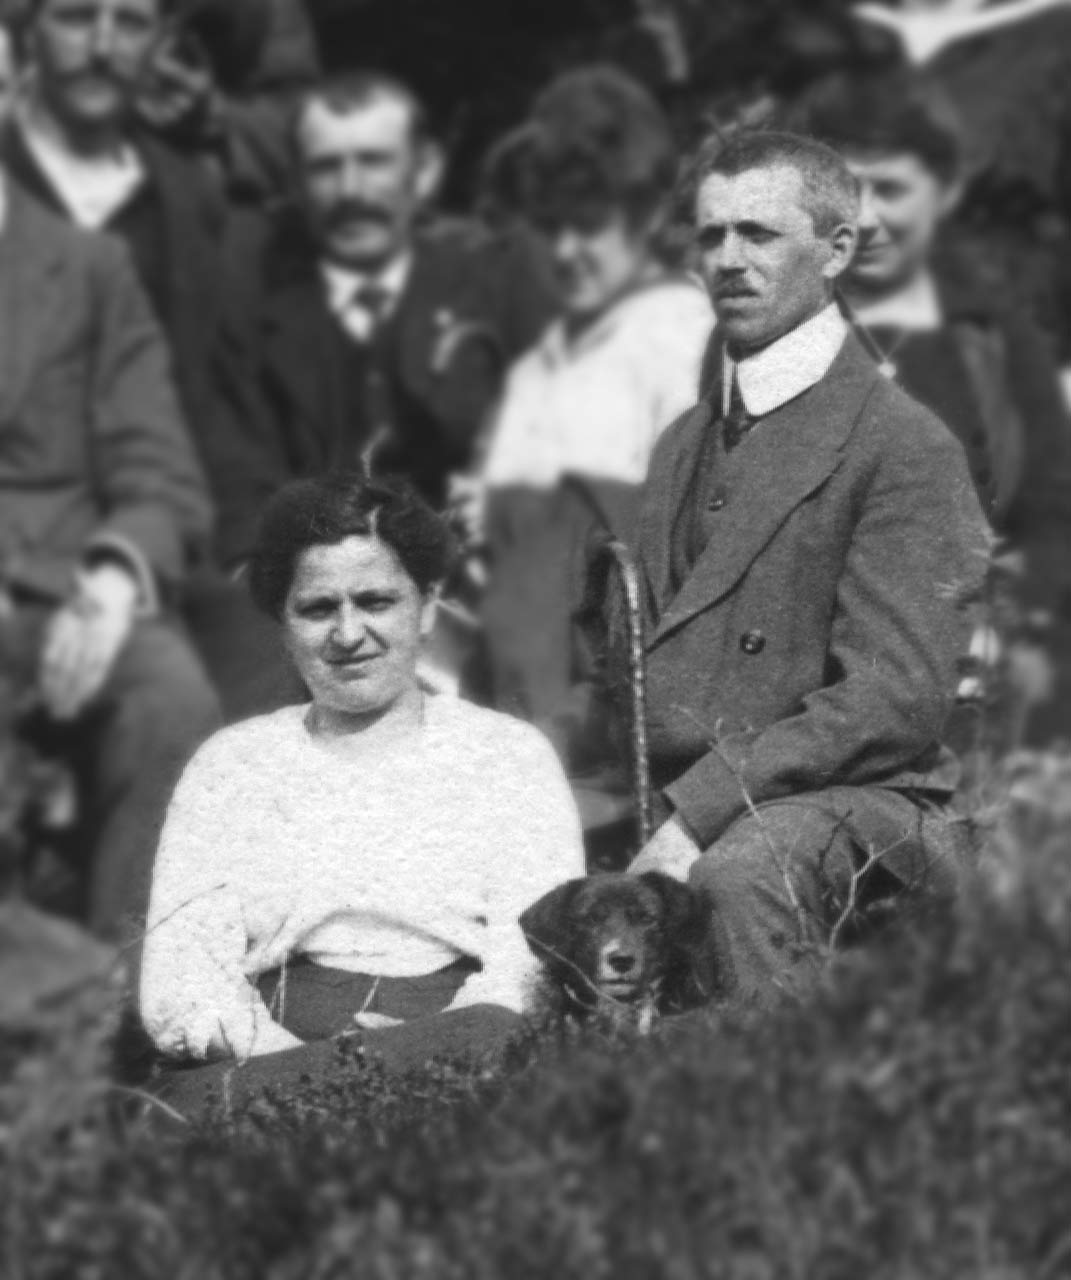
\includegraphics[width=5.609cm,height=6.705cm]{pictures/zulassungsarbeit-img024.jpg}

Emma und August Högn mit Jagdhund
„Treff“ bei einer Wanderung.\\
\end{supertabular}
\end{center}
\end{minipage}
\end{center}
Über den Zustand der Ehe Högns mit Emma ist kaum etwas bekannt.
Gerüchten zufolge soll Högns Ehefrau eine Affäre mit dem Nachbarn und
Kirchenchorsänger Rudolf Schwannberger gehabt haben.\footnote{
Interview Nr. 3, Ida Högn, 29.12.2002, Absatz 10} Ein möglicher Grund,
weshalb Högn kein zweites Mal geheiratet hat, könnte seine große Liebe
zu Emma gewesen sein. Ein weiterer Grund dafür dürfte auch seine
partnerschaftliche Beziehung zu Rosa Beischmied dargestellt haben, die
sich unweigerlich im Laufe der Jahre entwickelt hatte. Beide wurden als
eingespieltes Team beschrieben. \footnote{Interview Nr. 3, Ida Högn,
29.12.2002, Absatz 10} 35 Jahre lang begleitete Rosa Beischmied August
Högn bis zu seinem Tod und lebte mit ihm gemeinsam in derselben
Wohnung. \footnote{Interview Nr. 21, Lilo Leuze, 2.12.2004, Absatz 10;
Interview Nr. 20, Gertraud von Molo, 23.11.2004, Absatz 12} Je nach
Lebenslage unterstützte ihn die „Högn Rosl“, wie sie von einigen
Zeitzeugen genannt wurde, \footnote{Interview Nr. 2, Barbara Essigmann,
27.12.2002, Absatz 10, 76} etwa bei der Erziehung seines Sohnes, aber
auch beim Schuldienst, wenn zum Beispiel Högns Schüler Vitamintabletten
auf seine Anordnung hin, bei Rosa abholen mussten. \footnote{Interview
Nr. 6, Wilhelm Ederer, 2.1.2003, Absatz 34} Aber auch im Alter wurde
Högn von Rosa gepflegt, besonders nach seinem Schlaganfall.\footnote{
Dokument Nr. 73, Brief von August Högn an Stephan Leitner, 10.3.1961}
Nicht selbstverständlich und daher ebenso ein Indiz für das doch über
das rein Dienstliche hinausgehende Verhältnis zwischen Högn und
Beschmied war die Tatsache, dass Rosa Beischmieds „illegale“ Tochter
Mathilde, wie im Taufregister zu lesen ist, nach dem Tod ihrer
Großeltern in Högns Wohnung einziehen durfte. In der großen Wohnung im
Schulhaus erhielt sie ein eigenes Zimmer \footnote{Interview Nr. 19,
Mathilde Beischmied, 14.9.2004, Absatz 22} und fühlte sich von August
Högn sogar soweit akzeptiert, dass sie ihn heute als „Ersatzvater“
bezeichnet. \footnote{Interview Nr. 19, Mathilde Beischmied, 14.9.2004,
Absatz 18} Eine Anekdote, die Mathilde Beischmied in einem Interview
erzählte, mag vielleicht exemplarisch das gute und sehr
freundschaftliche Verhältnis Högns zu seiner Ziehtochter beleuchten und
Einblick ins damalige „Familienleben“ geben: Als Belohnung dafür, dass
die kleine Mathilde für Högn das Bier holte, bestand Högn darauf, dass
auch sie etwas von dem besorgten Getränk abbekam und fragte deshalb
ihre Mutter vorwurfsvoll: \zitat{„Kriegt sie heute kein
Bier?“ } \footnote{Interview Nr. 19, Mathilde Beischmied, 14.9.2004,
Absatz 6} Auch in der Funktion des Vaters, obwohl diese Bezeichnung
nicht zutrifft, zeigte sich Högn, als er für mehrere Jahre seine noch
schulpflichtige Enkelin Inge bei sich aufnahm. Als Grund, weshalb sie
zu ihrem Großvater kam, kann wohl die Trennung der ihrer Mutter Frieda
von ihrem ersten Ehemann und die neue Bekanntschaft mit ihrem späteren
Ehemann Dr. Karl Schlumprecht angesehen werden. \footnote{Interview Nr.
19, Mathilde Beischmied, 14.9.2004, Absatz 26} Da auch Högns Sohn Gustl
noch zu Hause wohnte, zählte Högns „neue Familie“ zusammen mit der
Enkelin Inge zeitweise sogar fünf Mitglieder.

\subsection{Chorregentendienst mit Unterbrechung}

Zum 1. September 1921 wurde, dem
Protokoll der Kirchenverwaltungssitzung zufolge, August Högn der
Chorregenten- und Organistendienst provisorisch übertragen.\footnote{
Dokument Nr. 116, Protokoll der Kirchenverwaltungssitzung, 21.8.1921}
Provisorisch steht hier nur deshalb, weil ein Jahr zuvor die gesetzlich
geregelte Verbindung zwischen Schul- und Kirchendienst, die mittels der
Chorregenten-, Organisten- und Mesnertätigkeiten der Lehrer bestand,
abgeschafft worden war. Besonders am Vormittag stattfindende
Beerdigungen standen der längerfristigen Weiterführung des
Organistendienst durch die Lehrer im Weg. Da viele Lehrer sich
freiwillig bereit erklärten, weiterhin Chorregent zu bleiben, ließ sich
diese jahrhunderte alte Tradition nicht von heute auf morgen
abschaffen. Den Schulbehörden blieb anscheinend nichts anderes übrig,
als den Chorregentendienst der Lehrer, verbunden mit den
Stundenausfällen, zumindest für eine gewisse Übergangszeit zu dulden.

\begin{center}
\begin{minipage}{9.491cm}
\begin{flushleft}
\tablefirsthead{}
\tablehead{}
\tabletail{}
\tablelasttail{}
\begin{supertabular}{m{4.8960004cm}m{4.196cm}}

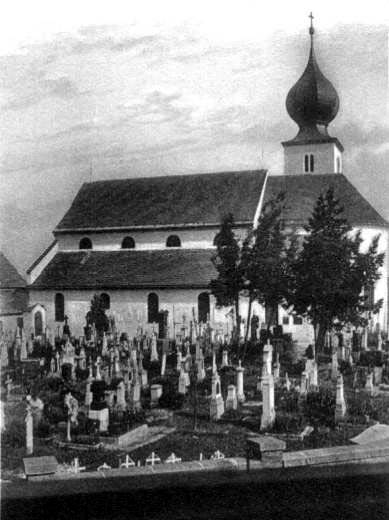
\includegraphics[width=4.713cm,height=6.301cm]{pictures/zulassungsarbeit-img025.jpg}

Pfarrkirche St. Laurentius zur Zeit von
August Högn &

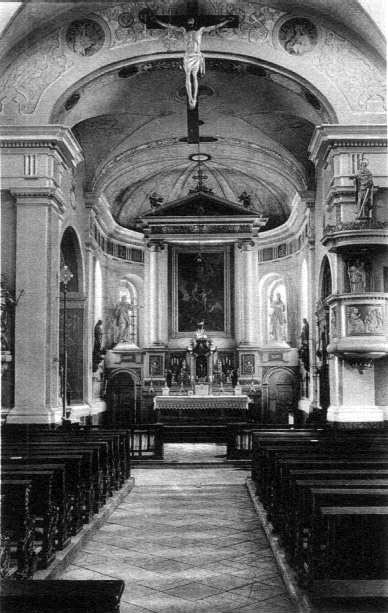
\includegraphics[width=4.013cm,height=6.292cm]{pictures/zulassungsarbeit-img026.jpg}

Blick zum Altarraum\\
\end{supertabular}
\end{flushleft}
\end{minipage}
\end{center}
Eine weitere Tradition, nämlich dass der Schulleiter den
Chorregentendienst übernahm, \footnote{Dokument Nr. 55, Artikel in der
Reicheneder-Chronik über August Högn} wurde in Ruhmannsfelden
fortgeführt, obwohl der Kirchendienst der Lehrer offiziell abgeschafft
wurde, als August Högn nach der Pensionierung des Bezirkshauptlehrers
Alois Auer 1921 \footnote{Reicheneder-Chronik, Pfarrmesner, Blatt 1
Vorderseite} nicht nur Chorregent, sondern
auch Schulleiter wurde. Max Weig war von 1879 bis zu seinem Tod 1895
Schulleiter und somit auch Organist und Chorregent.\footnote{
Reicheneder-Chronik, Schulwesen, Blatt 100
Rückseite}Erst im seinem Todesjahr kam vom
königlichen Bezirksamt Viechtach die Anweisung, dass ein Hilfslehrer
den Chorregentendienst übernehmen sollte. \footnote{Dokument Nr. 1,
Brief von Bezirkshauptmann Heerwagen an Kirchenverwaltung, 18.1.1895}
Von 1895 bis 1921 \footnote{Reicheneder-Chronik, Schulwesen, Blatt 110
Vorderseite} leitete Weigs Nachfolger, der Schulleiter Alois Auer,
zusammen mit seiner Frau Anna den Chor, ehe Högn ihn
fortführte. \footnote{Dokument Nr. 6, Brief von Max Rauscher sen. an
Kirchenverwaltung, 14.3.1927}

Vor allem aber dürften seine überdurchschnittlichen musikalischen
Fähigkeiten Högn dazu bestimmt haben, die alte Tradition des Lehrers
und Chorregenten in Personalunion weiterzuführen. Bevor er die
Kirchenchorleitung übernahm, hatte er über 20 lang Jahre als
guter \footnote{Dokument Nr. 48, Zeitungsartikel aus Viechtacher
Bayerwald-Bote, 2.8.1958} Tenor \footnote{Interview Nr. 5, Barbara
Essigmann, 2.1.2003, Absatz 40} und versierter Organist – man sagte von
ihm, dass er gleichzeitig singen, spielen und dirigieren
konnte \footnote{Interview Nr. 16, Maria Freisinger, 25.8.2004, Absatz
28} – in verschiedenen Orten an der Kirchenmusik mitgewirkt und
Erfahrungen gesammelt. \footnote{Dokument Nr. 18, Brief von August Högn
an Pfarrer Reicheneder, 25.1.1954} Nicht nur im Manualspiel war er
gewandt, wie die virtuos gesetzte Fassung seines Marsches „In Treue
fest!“ für Klavier zu zwei Händen beweist, sondern auch mit dem
Pedaleinsatz konnte er von seinem Können überzeugen.\footnote{
Interview Nr. 4, Maria Schröck, 30.12.2002, Absatz 58} Unter seinen
Stücken, die er auf der Orgel spielte, war die berühmte und nicht
gerade leicht zu spielende Toccata und Fuge in d-moll von Johann
Sebastian Bach. Angesichts einer derart gehoben Orgelliteratur, die zu
seinem Repertoire gehörte, überrascht es daher nicht, wenn manche
Kirchenbesucher so lange in der Kirche blieben, um Högns Orgelspiel bis
zum Schluss beiwohnen zu. \footnote{Interview Nr. 11, Josef Stern,
21.2.2003, Absatz 2} Nicht zu vergessen sind auch seine
kompositorischen Fähigkeiten: Innerhalb von wenigen Tagen konnte er für
den Einsatz in der Kirchenmusik passende Kompositionen schreiben. Ein
befreundeter Chorleiter bat Högn in einem Brief, ein Stück für seinen
Männerchor zu schreiben. \footnote{Dokument Nr. 62, Brief von „Franzl“,
Regen an August Högn, 17.6.1928} Laut einem Vermerk auf der
betreffenden Komposition wurde das Stück schon zwei Tage später fertig
gestellt. Kein Wunder also, dass seine musikalischen Leistungen auch im
Urteil seiner Zeitgenossen lobende Anerkennung fanden. Bischof
Buchberger zum Beispiel hob bei einer Firmung hervor, dass er selten
einen so guten Organisten Orgel spielen gehört habe.\footnote{
Interview Nr. 13, Lorenz Schlagintweit, 29.11.2003, Absatz 2} Josef
Brunner, der als Organist an der Kirchenmusik unter Högn mitwirkte,
meinte sogar: \zitat{„Der Högn war ein selten guter Musiker.
So einer steht nicht mehr auf.“ } \footnote{Interview Nr. 8, Josef
Brunner, 3.1.2003, Absatz 16}

\zitat{„Zur größten Zufriedenheit der ganzen Kirchengemeinde“}
\footnote{Dokument Nr. 12, Brief von Kirchenverwaltung an Regierung
von Niederbayern, 1.4.1927} leitete August Högn laut Pfarrer Fahrmeier
den Kirchenchor bis Ende 1924 und ein Ruhmannsfeldener Bürger, der die
Entwicklung des Kirchenchors über einen längeren Zeitraum beurteilen
konnte, bestätigte, dass der Chor, der unter dem Lehrer Weig
\zitat{„einen guten Namen hatte,“ } \footnote{Dokument Nr. 6,
Brief von Max Rauscher sen. an Kirchenverwaltung, 14.3.1927} und unter
der Leitung von Anna Auer \zitat{„einen Niedergang“
} \footnote{Dokument Nr. 6, Brief von Max Rauscher sen. an
Kirchenverwaltung, 14.3.1927} erlebte, bei Högn wieder eine
\zitat{„Verbesserung erfuhr.“ } \footnote{Dokument Nr. 6,
Brief von Max Rauscher sen. an Kirchenverwaltung, 14.3.1927} Högn wäre
sicher weit länger als drei Jahre Leiter der Kirchenmusik geblieben,
hätte sich nicht ein Nachfolger geradezu angeboten, der es ermöglichte,
dass auch in Ruhmannsfelden die Trennung von Schul- und Kirchendienst
der Lehrer vollzogen wurde. Der 20-jährige Max Rauscher stammte aus
einer sehr musikalischen Familie, die nahe an der Pfarrkirche eine
kleine Konditorei mit Café führte. \footnote{Interview Nr. 16, Maria
Freisinger, 25.8.2004, Absatz 48} Nach Abschluss der
Kirchenmusikausbildung war das am 14.12.1924 \footnote{Dokument Nr.
118, Protokoll der Kirchenverwaltungssitzung, 14.12.1924} in der
Kirchenverwaltungssitzung beschlossene Engagement am Heimatort für
Rauscher sicher der bequemste Weg, eine Stelle zu bekommen.

Weniger überraschend ist die Tatsache, dass das Beschäftigungsverhältnis
des jungen Rauscher an seinem Heimatort, wo seit Jahrzehnten
ausnahmslos ältere Volksschullehrer den Kirchendienst tätigten, nur von
kurzer Dauer war. Nörgler, die schon zu Beginn von Rauschers Tätigkeit
wenig Vertrauen in ihn setzten, \footnote{Dokument Nr. 6, Brief von Max
Rauscher sen. an Kirchenverwaltung, 14.3.1927} sahen sich sicher
bestätigt, als dieser kaum zwei Jahre nach seiner Anstellung ein in
ihren Augen unerhörte Gehaltserhöhung von mehr als 150 Mark zusätzlich
zu den 33 Mark, in ihm monatlich bezahlt wurden, bei Pfarrer Fahrmeier
einforderte. Pfarrer Fahrmeiers Reaktion war eindeutig: Er drohte mit
Kündigung. Von der Drohung unbeeindruckt, wandte sich Rauscher an das
Bischöfliche Ordinariat Regensburg, um seinem Wunsch nach
Gehaltserhöhung Nachdruck zu verleihen. \footnote{Dokument Nr. 2, Brief
von Max Rauscher an Bischöfliche Ordinariat Regensburg, 4.11.1926} Als
Fahrmeier von der Eingabe an das Bischöfliche Ordinariat Regensburg
erfuhr, stellte er Rauscher \zitat{„vor versammelter
Sängerschar“}  \footnote{Dokument Nr. 3, Brief von Max Rauscher an
Pfarrer Fahrmeier, 15.11.1926} zur Rede und provozierte einen offenen
Streit. Verärgert über diese öffentliche Demütigung betonte Rauscher in
seinem Brief an Fahrmeier vom 15.11.1926, dass diese vollkommen
unangebracht war, und behauptete, dass eine Zurechtweisung
\zitat{„zur Zeit von Lehrer Högn“ } \footnote{Dokument Nr. 3,
Brief von Max Rauscher an Pfarrer Fahrmeier,
15.11.1926}\zitat{ }passend gewesen wäre, als
\zitat{„nicht bloß Lektüre während des Gottesdienstes
gelesen, sondern von seiner Tochter Liebeleien getrieben und Schokolade
gegessen wurden.“ } \footnote{Dokument Nr. 3, Brief von Max Rauscher an
Pfarrer Fahrmeier, 15.11.1926} Högn konnte natürlich diese
Anschuldigungen nicht auf sich sitzen lassen. Die
\zitat{„ungezogenen Anschuldigungen“} verurteilte er in einem
Brief an Pfarrer Fahrmeier aufs Schärfste und ersuchte
\zitat{„in der Wahrung der Autorität und im Ansehen unseres
hoch verdienten und beliebten H. H. Pfarrer Fahrmeier Max Rauscher zu
kündigen, damit endlich diesem unerhörten Treiben dieses jungen Mannes
Einhalt geboten ist und nicht derselbe und noch andere mit in der
Selbstüberhebung und Geringeinschätzung anderer gestärkt werden.“
} \footnote{Dokument Nr. 4, Brief von August Högn an Kirchenrat, Dez.
1926} Wie zu erwarten war, wurde dem Chorregenten Max Rauscher zum 1.
Januar 1927 gekündigt, ihm aber ein neuer Dienstvertrag in Aussicht
gestellt, unter der Vorraussetzung, dass er auf seine
Gehaltsforderungen verzichtet und in der
\zitat{„Kirchenratssitzung Abbitte leistet.“ }\footnote{
Dokument Nr. 5, Protokoll der Kirchenverwaltungssitzung, 30.12.1926} Da
man beim Lesen der entsprechenden Korrespondenz deutlich erkennt, dass
es Rauscher von Anfang an ganz bewusst auf die Kündigung angelegt
hatte, wundert es keinen nicht, als er sich in der Kirchenratssitzung,
in der er Abbitte leisten sollte, nicht gemäß den Vorstellungen der
Pfarroberen verhielt und ihm deshalb endgültig gekündigt
wurde. \footnote{Dokument Nr. 12, Brief von der Kirchenverwaltung an
die Regierung von Niederbayern, 1.4.1927}

\begin{center}
\begin{minipage}{4.591cm}
\begin{center}
\tablefirsthead{}
\tablehead{}
\tabletail{}
\tablelasttail{}
\begin{supertabular}{m{4.3910003cm}}

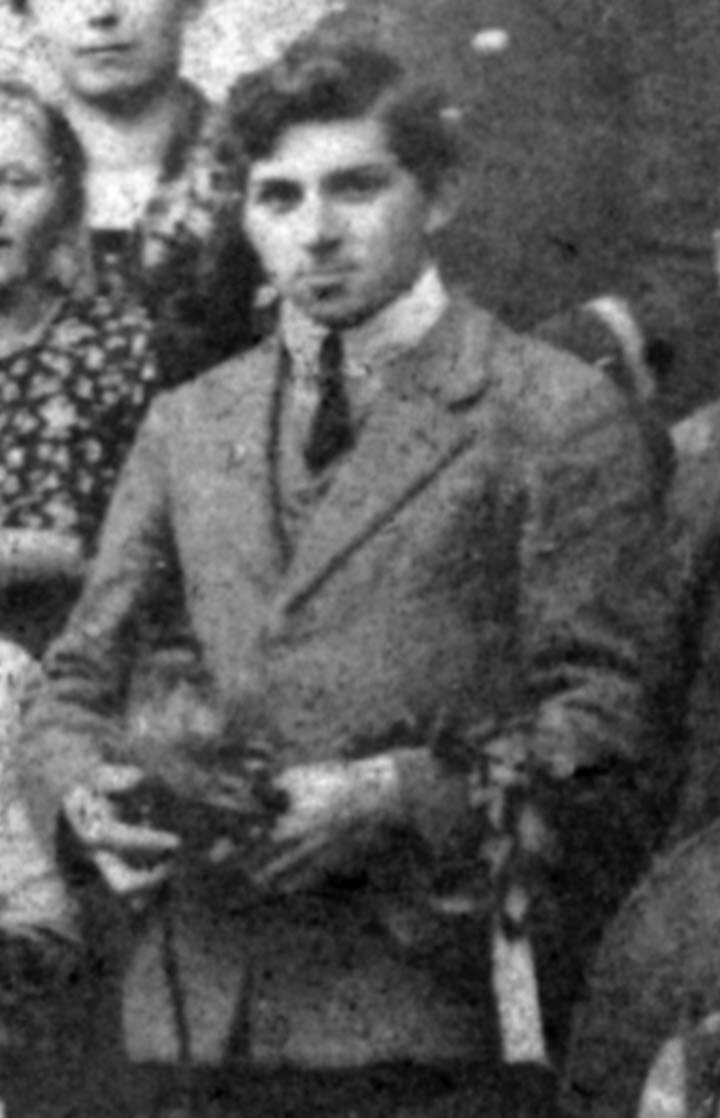
\includegraphics[width=4.209cm,height=6.507cm]{pictures/zulassungsarbeit-img027.jpg}

Max Rauscher\\
\end{supertabular}
\end{center}
\end{minipage}
\end{center}
Als Rauscher durch seine Anschuldigung Högn in den Streit mit hineinzog
und dieser mit markigen Worten offen die Kündigung Rauschers verlangte,
wurde eines deutlich: Ihr Verhältnis zueinander war offenbar auch
vorher nicht gut gewesen. Gehörte Högn nicht auch zu den Nörglern, die
schon zu Beginn von Rauschers Dienstzeit wenig Vertrauen in ihn setzten
und Rauscher während seiner 2-jährigen Dienstzeit die Arbeit schwer
machten, bis er es schließlich mit einer utopischen Gehaltforderung
bewusst auf die Kündigung anlegte? Högn wäre mit Sicherheit gerne
weiterhin Chorregent geblieben, wenn man, abgesehen vom finanziellen
Aspekt, die Abwechslung in der Tätigkeit betrachtet, die der
Chorregentendienst bot, sowie die Tatsache, dass Högn diesen Dienst mit
Leib und Seele ausführte. Die Anstellung Rauschers lieferte
letztendlich den Grund dafür, dass Kirchen- und Schuldienst nicht mehr
von einer Person ausgeübt werden durfte.

Eine Eintragung von Högn in einer Dirigierpartitur aus dem Notenbestand
der Ruhmannsfeldener Kirche ist beredtes Zeugnis dieser Rivalität
zwischen Rauscher und Högn. Rauscher hatte einen vermeintlichen
Vorzeichenfehler in der Partitur einer Messe von Vinzenz Goller
korrigiert. In einem rechthaberischen Ton schrieb Högn, der von der
Richtigkeit des gedruckten Notentextes überzeugt war, später den
Kommentar \zitat{„Grober Fehler! Nein! Muss „des“ heißen!“
}(Abb. 26) dazu, anstatt das eingefügte Vorzeichen einfach
auszuradieren, als hätte er der Nachwelt seine Zweifel an Rauschers
Kompetenz durch die Eintragung in die Partitur, die eigentlich nur er
selbst verwendete, mitteilen wollen.

\begin{center}
\begin{minipage}{4.142cm}
\begin{flushleft}
\tablefirsthead{}
\tablehead{}
\tabletail{}
\tablelasttail{}
\begin{supertabular}{m{3.9420002cm}}

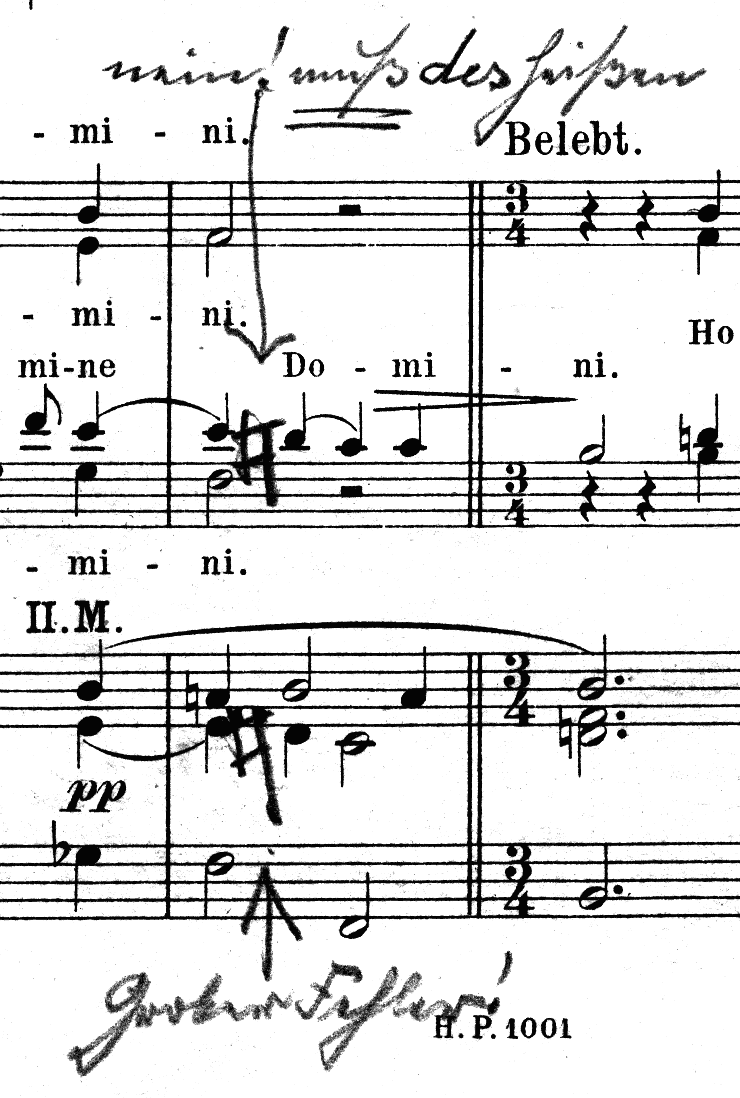
\includegraphics[width=3.759cm,height=5.547cm]{pictures/zulassungsarbeit-img028.png}

Eintragungen
von Max Rauscher und August Högn in eine Dirigierparitur\\
\end{supertabular}
\end{flushleft}
\end{minipage}
\end{center}
Pfarrer Fahrmeier schrieb nach der Kündigung Rauschers an die Regierung
von Niederbayern einen Brief, der den Zweck erfüllen sollte, eine
Ausnahmegenehmigung für die Übernahme des Chorregentendienstes durch
Högn zu erhalten. Dies zeigt, dass das Verhältnis Fahrmeier und Högn
anscheinend ein sehr gutes war. Nur Högn besitze, diesem Schreiben
zufolge die, \zitat{„zur Übernahme des Kirchenchores
notwendigen musikalischen Fähigkeiten und Kenntnisse“ }\footnote{
Dokument Nr. 12, Brief von der Kirchenverwaltung an die Regierung von
Niederbayern, 1.4.1927} und daher solle die zuständige Behörde den
Chorregentendienst von Högn \zitat{„bis auf weiteres“
} \footnote{Dokument Nr. 12, Brief von der Kirchenverwaltung an die
Regierung von Niederbayern, 1.4.1927} genehmigen. August Högn kannte
Fahrmeier schon lange vor seiner Ruhmannsfeldener Zeit. In Deggendorf
war Fahrmeier als Geistlicher zwischen 1896 und 1918 tätig.\footnote{
Reicheneder-Chronik, Seelsorger, Blatt III/13
(1) Vorderseite} Er konnte als Freund und Hauspfarrer der Familie Högn
in Deggendorf bezeichnet werden. Wenn er zur Ruhmannsfeldener Zeit
einen Ausflug nach Deggendorf unternahm, genehmigte er sich stets im
Hause Högn zuerst ein Bad, bevor er seinen Besorgungen in der Stadt
nachging. \footnote{Interview Nr. 3, Ida Högn, 29.12.2002, Absatz 10}

August Högns zweites Engagement in der Kirche von Ruhmannsfelden sollte
nur von begrenzter Dauer sein. Nur bis zu den Sommerferien 1927 sollte
die Regierung von Niederbayern Högns kirchenmusikalische Tätigkeit
genehmigen, \footnote{Dokument Nr. 13, Brief von der Kirchenverwaltung
an die Regierung von Niederbayern, 22.4.1927} bis ein pensionierter
Lehrer gefunden war, der die Chorregentenstelle längerfristig
übernehmen könnte. Doch unter der Ruhmannsfeldener Bevölkerung erhob
sich heftiger Widerstand gegen die Anstellung eines
Pensionisten, \footnote{Dokument Nr. 14, Brief von Alois Hartl an
Kirchenrat, 15.6.1927; Dokument Nr. 15, Brief von Johann Bielmeier an
Kirchenverwaltung, 17.6.1927} sodass die Stelle öffentlich
ausgeschrieben und von den fünf Kirchenmusiker, \footnote{Dokument Nr.
75, Bewerbung von Gottfried Hagemeiner, 25.10.1927} die sich beworben
hatten, entschied man sich für einen gewissen Georg Roßnagel. Sein
Dienstvertrag wurde zum Unterschreiben für den 7. Juni 1927 aufgesetzt.
Anscheinend hat Roßnagel seinen Dienst nie angetreten, denn derselbe
Dienstvertrag wurde zu einem späteren Zeitpunkt, mit ausgebesserten
Namen noch einmal bei der Anstellung von Albert Schroll verwendet, der
am 31. Juli 1929 diesen Vertrag mit der Kirche in Ruhmannsfelden
abschloss. Während der Name Schroll bei vielen Zeitzeugen bekannt war,
wusste nie etwas von einem Kirchenmusiker mit dem Namen Georg Roßnagel,
der laut Dienstvertrag zwei Jahre lang in Ruhmannsfelden gewirkt haben
soll. \footnote{Dokument Nr. 8, Dienstvertrag für Albert Schroll (Georg
Roßnagel), 31.7.1929 (7.6.1927)} Im Sommer 1929 trat Albert Schroll den
Chorregentendienst in Ruhmannsfelden an. Die auf wenige Wochen
beschränkte Aushilfe durch August Högn hat man am Ende auf über zwei
Jahre verlängert.

\begin{center}
\begin{minipage}{9.638cm}
\begin{center}
\tablefirsthead{}
\tablehead{}
\tabletail{}
\tablelasttail{}
\begin{supertabular}{m{4.333cm}m{4.905cm}}

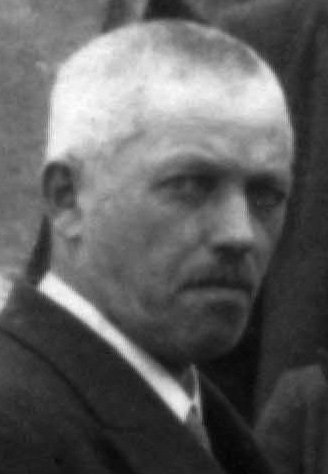
\includegraphics[width=4.15cm,height=6.006cm]{pictures/August-Hoegn_Nachruf.jpg}

August Högn &

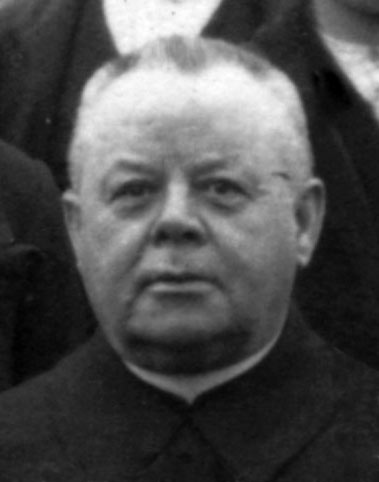
\includegraphics[width=4.722cm,height=5.994cm]{pictures/zulassungsarbeit-img029.jpg}

Karl Fahrmeier, in Ruhmannsfelden
Pfarrer von 1918 – 1935\\
\end{supertabular}
\end{center}
\end{minipage}
\end{center}

\subsection{Der Lehrer und Schulleiter}

1929 wurde August Högn zum
Oberlehrer ernannt. Dieser höhere Dienstgrad hatte ebenso wie seine
Ernennung zum Rektor 1940 bezüglich seines Aufgabenfeldes in der Schule
keinen Einfluss, da er schon seit 1921 Schulleiter war. Es war sicher
zur damaligen Zeit keine leichte Aufgabe, die Landschule zu leiten. Zum
einem war die finanzielle Lage der beteiligen Gemeinden, der so
genannten Schulsprengelverwaltung ziemlich angespannt, die für die
Instandsetzung der Schulgebäude einschließlich der Lehrerwohnungen und
die Beschaffung von Lehrmittel zuständig war. \footnote{Dokument Nr.
146, Brief von August Högn an Bürgermeister Forster, Ruhmannsfelden,
18.5.1936}

Zu manchen Zeiten wurden nicht einmal die notwendigen Lehrmittel im
erforderlichen Maße bereitgestellt. \footnote{Dokument Nr. 146, Brief
von August Högn an Bürgermeister Forster, Ruhmannsfelden, 18.5.1936}
Die finanziellen Engpässe wirkten sich natürlich ebenso auf den Zustand
der Schulgebäude aus. So konnten beispielsweise im Jahr 1934 die
Toiletten im so genannten Mädchenschulhaus eine Zeit lang gar nicht
mehr benutzt werden, da sie derart baufällig waren, dass laut Högn ihre
Benutzung lebensgefährlich für die Kinder war. \footnote{Dokument Nr.
144, Brief von August Högn an verstärkten Gemeinderat Ruhmannsfelden,
13.9.1934} Zum anderem schlug sich die schwierige Erwerbslage vieler
Familien negativ auf das Lernklima nieder. Besonders zur Erntezeit
mussten viele Kinder in der Landwirtschaft ihrer Eltern mithelfen, da
sich kaum eine Familie eine zusätzliche Arbeitskraft leisten konnte.
Aus diesem Grund war es zeitweise üblich, dass in den Sommermonaten der
Unterricht gekürzt werden musste. \footnote{Interview Nr. 6, Wilhelm
Ederer, 2.1.2003, Absatz 30} Eine dauerhafte Belastung für den
Schulbetrieb waren die langen Schulwege, die die Schüler aus am Rande
des großen Schulsprengels gelegenen Ortschaften und Höfen zu Fuß
zurücklegen mussten. Über eine Stunde dauernde Märsche zur Schule waren
keine Seltenheit und wurden bei Regen oder Schnee für die Schüler zur
Tortur. \footnote{Interview Nr. 6, Wilhelm Ederer, 2.1.2003, Absatz 10}

\begin{center}
\begin{minipage}{10.931cm}
\begin{flushleft}
\tablefirsthead{}
\tablehead{}
\tabletail{}
\tablelasttail{}
\begin{supertabular}{m{10.731cm}}

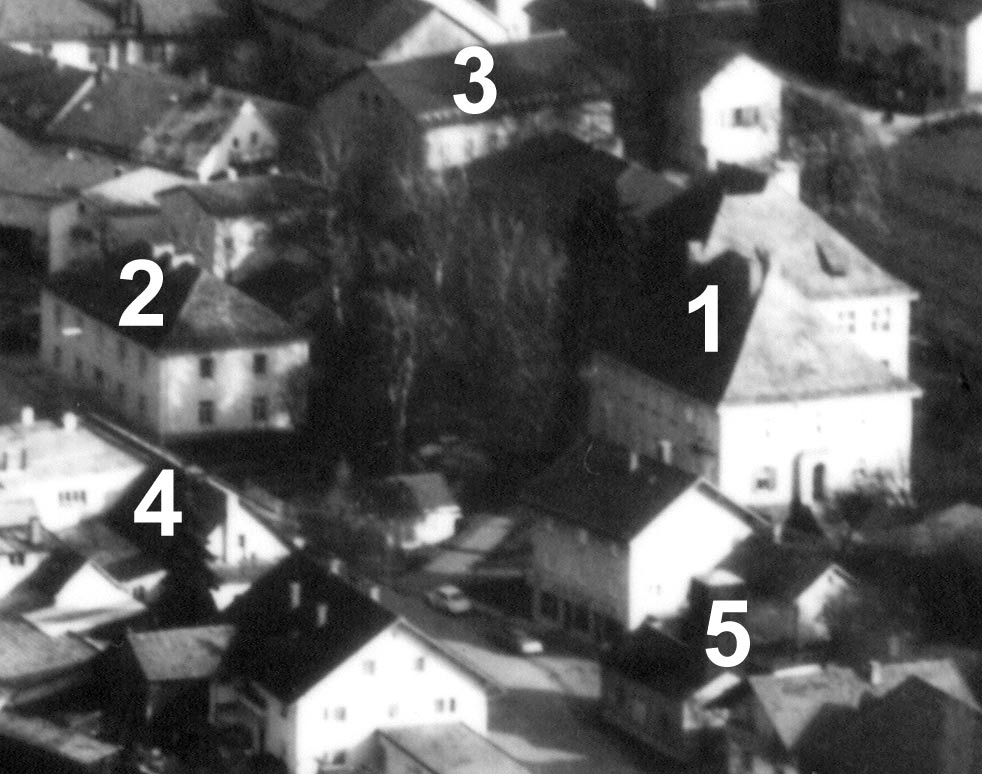
\includegraphics[width=10.548cm,height=8.313cm]{pictures/zulassungsarbeit-img030.jpg}

Schul- und Wohnhäuser von Högn:
\textbf{1:} Schulhaus von 1908: Hier wohnte August Högn 1932 – 1945,
\textbf{2:} Knabenschulhaus von 1834: Wohnung 1910 – 1932, \textbf{3:}
Mädchenschulhaus von 1884, \textbf{4:} Härtl-Haus: Wohnung 1945 – 1961,
\textbf{5:} Feuerwehrhaus\\
\end{supertabular}
\end{flushleft}
\end{minipage}
\end{center}
Wahrscheinlich lag es an den damals geringeren Anforderungen, die man an
eine Landschule stellte – überspitzt formuliert, war man schon froh,
wenn die Schüler regelmäßig am Unterricht teilnahmen – und an der
Positionen Högns als Schulleiter, dass er sich gewisse Dinge erlauben
konnte, die nicht regelkonform waren und in der heutigen Zeit undenkbar
wären. So ließ er beispielsweise die Schüler nicht nur für schulische
Zwecke, sondern auch für seine Privatangelegenheiten kleine Dienste und
Arbeiten während der Unterrichtszeit erledigen. Zu diesen Arbeiten
gehörten unter anderem einen Zettel von Klassenzimmer zu Klassenzimmer
tragen, \footnote{Interview Nr. 4, Maria Schröck, 30.12.2002, Absatz
46} Lehrmittel aus dem entsprechenden Zimmer holen, \footnote{Interview
Nr. 14, Johann Freisinger, 29.12.2003, Absatz 26} den Schulhof
aufräumen, das Pflaster am der Schule nahe gelegenen Kriegerdenkmal
ausgrasen \footnote{Interview Nr. 4, Maria Schröck, 30.12.2002, Absatz
14} und Holzaufrichten. \footnote{Korrespondenz Nr. 26, Brief von Franz
Danziger an Josef Friedrich, 25.2.2003; Interview Nr. 17, Max Holler,
26.8.2004, Absatz 16} Dies waren Dienste, die mit der Schule einen
gewissen Zusammenhang hatten, aber die Teppiche aus Högns Wohnung
klopfen, \footnote{Interview Nr. 6, Wilhelm Ederer, 2.1.2003, Absatz
34} von Högn geschossenes Wildfleisch zum Bahnhof bringen,\footnote{
Interview Nr. 17, Max Holler, 26.8.2004, Absatz 8} sein Rad
putzen \footnote{Interview Nr. 14, Johann Freisinger, 29.12.2003,
Absatz 24} oder sogar es reparieren \footnote{Interview Nr. 17, Max
Holler, 26.8.2004, Absatz 8} waren Arbeiten, die rein ins Private
fielen und jeden Bezug zur Schule entbehrten. Diese Tätigkeiten wurden
aber nicht als Strafarbeit, sondern als Zeichen besonderen Vertrauens
verstanden. \footnote{Korrespondenz Nr. 26, Brief von Franz Danziger an
Josef Friedrich, 25.2.2003}

{\centering
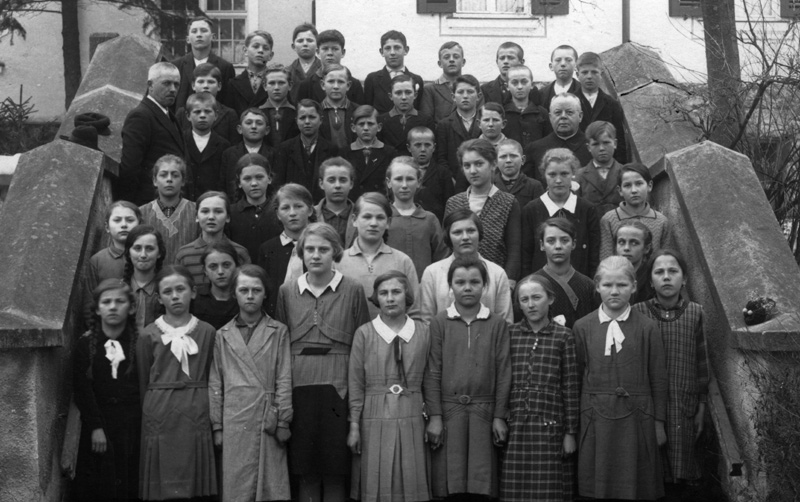
\includegraphics[width=16.044cm,height=10.081cm]{pictures/zulassungsarbeit-img031.jpg}
 \par}
Klassenfoto von 1932 mit August Högn
(links) und Pfarrer Fahrmeier (rechts)

Seitdem 1920 der Kirchendienst der Lehrer abgeschafft wurde, war der
Einsatz Högns als Organist bei Beerdigungen während der Unterrichtszeit
ein eindeutiger Verstoß gegen das damalige Schulrecht. Dass diese
Praxis auch noch zur NS-Zeit von den Behörden und der Seite der Eltern
toleriert wurde, lag an der besonders großen Macht der Institution
Kirche am Land. Eine gewöhnliche Beerdigung dauerte von 9 bis 11 Uhr,
so genannte „levitierte“ Beerdigungen für wohlhabende Verstorben
dauerten wesentlich länger. \footnote{Interview Nr. 4, Maria Schröck,
30.12.2002, Absatz 10} Högns Schüler mussten während seiner Abwesenheit
in Stillarbeit Aufgaben erledigen, ein paar Schüler wurden zu
Aufpassern ernannt \footnote{Interview Nr. 6, Wilhelm Ederer, 2.1.2003,
Absatz 8, Interview Nr. 4, Maria Schröck, 30.12.2002, Absatz 12;} und
die Lehrer der benachbarten Klassen statteten der „verwaisten Klasse“
hin und wieder einen Besuch ab. \footnote{Interview Nr. 4, Maria
Schröck, 30.12.2002, Absatz 10} Natürlich verhielten sich die Schüler
nicht nach Högns Vorstellung. Tumult im Klassenzimmer war noch das
kleinere Übel. Manchmal kam es sogar vor, dass sich einige Schüler
bereits auf den Nachhauseweg gemacht hatten, ehe Högn von der Kirche
ins Klassenzimmer zurückkehrte. Högn soll bei derartigen Vorkommnissen
des Öfteren versucht haben, diese Schüler mit dem Fahrrad einzuholen
und sie so zur Schule zurückzubringen. \footnote{Interview Nr. 6,
Wilhelm Ederer, 2.1.2003, Absatz 8}

\begin{center}
\begin{minipage}{6.202cm}
\begin{center}
\tablefirsthead{}
\tablehead{}
\tabletail{}
\tablelasttail{}
\begin{supertabular}{m{6.0020003cm}}

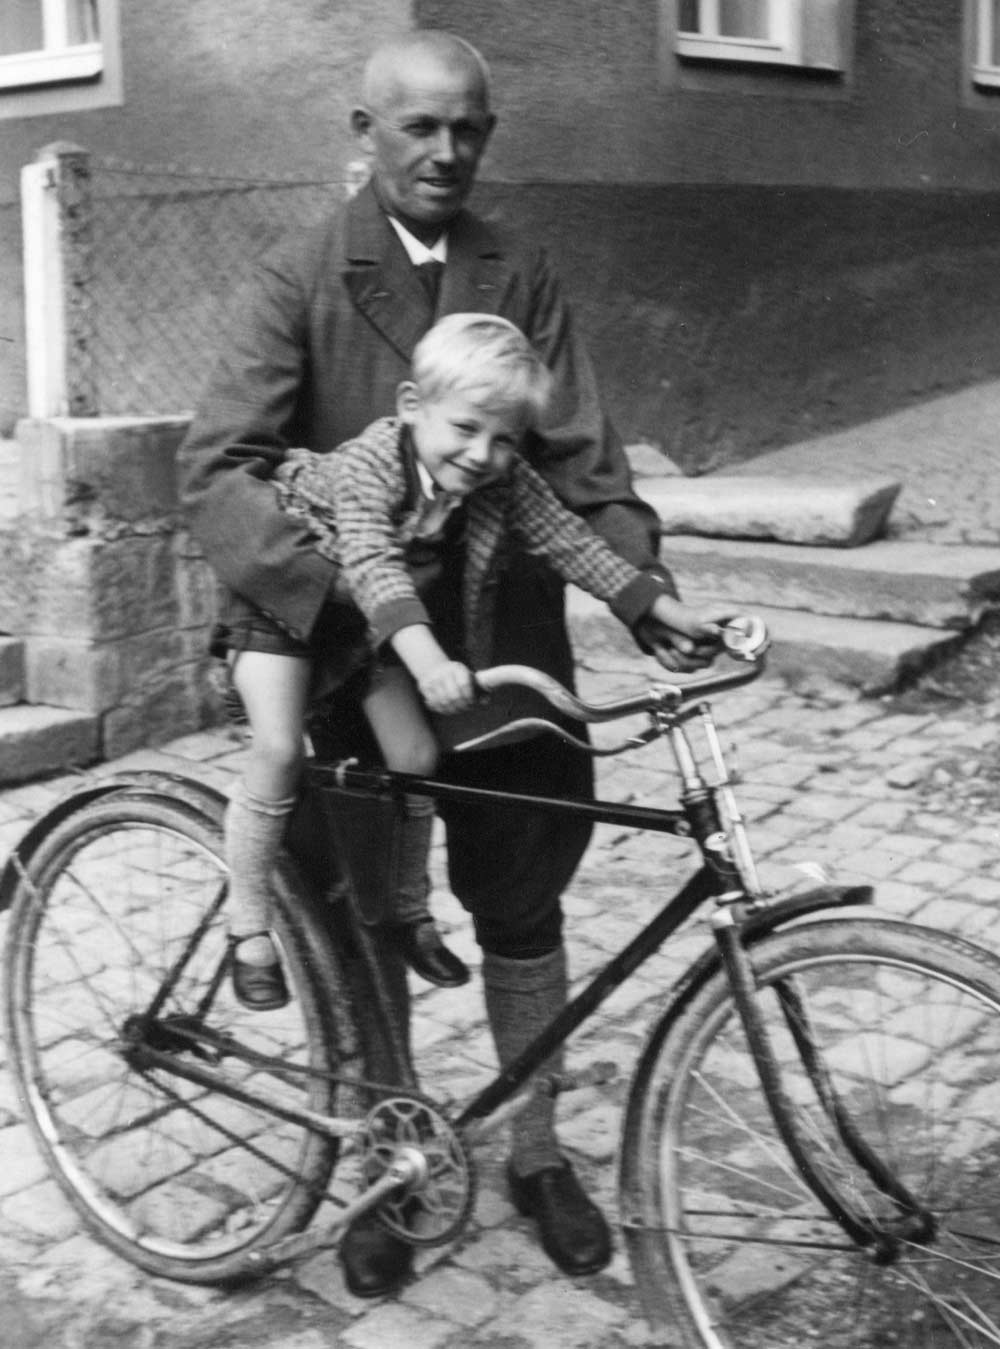
\includegraphics[width=5.821cm,height=7.851cm]{pictures/zulassungsarbeit-img032.jpg}

August Högn mit Enkel Werner
Schlumprecht und seinem Fahrrad 1939\\
\end{supertabular}
\end{center}
\end{minipage}
\end{center}
Die alltäglichen Beschwerlichkeiten, mit denen der damalige Lehrerstand
über all in Bayern zu kämpfen hatte – man bedenke die große
Schüleranzahl in einer Klasse – und die besonderen Schwierigkeiten in
Ruhmannsfelden schienen sich unter anderem auch in der Art
niedergeschlagen zu haben, wie Högn in der Klasse für Disziplin sorgte.
Viele der befragten Zeitzeugen bezeichneten August Högn als strengen
Lehrer. \footnote{Interview Nr. 3, Ida Högn,
29.12.2002, Absatz 6; Interview Nr. 14, Johann Freisinger, 29.12.2003,
Absatz 2; Interview Nr. 17, Max Holler, 26.8.2004, Absatz 16; Interview
Nr. 5, Barbara Essigmann, 2.1.2003, Absatz 18; Interview Nr. 24, Johann
Glasschröder, 28.12.2004, Absatz 12, 28} Dass er unfolgsame Schüler
mit Ohrfeigen, Tatzen \footnote{Interview Nr. 17, Max Holler,
26.8.2004, Absatz 12}, Ziehen an den Haarspitzen \footnote{Interview
Nr. 5, Barbara Essigmann, 2.1.2003, Absatz 20} und Schlägen auf den
Hintern \footnote{Interview Nr. 5, Barbara Essigmann, 2.1.2003, Absatz
18} bestrafte, ist daher kaum verwunderlich und außerdem üblich für die
damalige Zeit. Noch gewalttätigere Maßnahmen sind von ehemaligen
Schülern als Zeichen einer gewissen Hilflosigkeit verstanden worden,
die sie beim alternden und überforderten Lehrer beobachten konnten.
Hierzu gehörten Strafen, wie zum Beispiel Schülern die Schiefertafel so
stark über den zu Kopf schlagen, dass sie zerbrach, \footnote{Interview
Nr. 3, Ida Högn, 29.12.2002, Absatz 6} einen Bund mit vielen Schlüsseln
über den Kopf schlagen, \footnote{Interview Nr. 14, Johann Freisinger,
29.12.2003, Absatz 6} den Kopf der Schüler an die Tafel
stoßen, \footnote{Interview Nr. 14, Johann Freisinger, 29.12.2003,
Absatz 26; Interview Nr. 6, Wilhelm Ederer, 2.1.2003, Absatz 16} oder
sogar mit einem Blumentopf nach einem Schüler werfen.\footnote{
Interview Nr. 14, Johann Freisinger, 29.12.2003, Absatz 28} Ebenso gut
passen ungewöhnlich scharfe Beschimpfungen der Schüler mit Ausdrücken
wie etwa „ordinärer Hund“, \footnote{Interview Nr. 6, Wilhelm Ederer,
2.1.2003, Absatz 16} „dreckiger Hundschuft“ \footnote{Interview Nr. 17,
Max Holler, 26.8.2004, Absatz 16} oder „blöder Hammel“ \footnote{
Interview Nr. 5, Barbara Essigmann, 2.1.2003, Absatz 20} zum Bild des
alternden und überforderten Lehrers. Doch nicht nur mit harten Strafen,
die sich fester ins Gedächtnis ehemaliger Schüler eingruben, als
mancher pädagogische Kniff, versuchte er für Ruhe im Klassenzimmer zu
sorgen. Als geschickter Lehrer zeigte er sich, wenn er die Schüler am
Ende jeder Unterrichtsstunde zur Entspannung und Auflockerung aufstehen
ließ, um ihre überschüssigen Energien vor und nicht während der Stunde
loszuwerden. \footnote{Korrespondenz Nr. 26, Brief von Franz Danziger
an Josef Friedrich, 25.2.2003} Das negative Bild vom strafenden Lehrer
hebt sich auf, wenn Zeitzeugen ihren ehemaligen Lehrer trotz aller
seiner Wutausbrüche als sehr gerechten Lehrer bezeichnen.\footnote{
Interview Nr. 24, Johann Glasschröder, 28.12.2004, Absatz 12}

Als Entschädigung für manche Schwierigkeit im Schulalltag galt für den
leidenschaftlichen Musiker sicher der Musikunterricht. Dieser hatte den
größten Stellenwert unter allen Fächern, die Högn
unterrichtete. \footnote{Interview Nr. 17, Max Holler, 26.8.2004,
Absatz 10; Interview Nr. 4, Maria Schröck, 30.12.2002, Absatz 10;
Korrespondenz Nr. 26, Brief von Franz Danziger an Josef Friedrich,
25.2.2003} Zu manchen Zeiten wurde jeden Tag eine Stunde
gesungen. \footnote{Interview Nr. 5, Barbara Essigmann, 2.1.2003,
Absatz 20} Selbst als kurz vor Ende des 2. Weltkriegs ein Lehrer zwei
Klassen unterrichten musste – eine Klasse hatte täglich nur drei
Stunden Unterricht – wurde jeden Tag vor Beginn des Unterrichts statt
des Gebets ein Lied gesungen. \footnote{Interview Nr. 16, Maria
Freisinger, 25.8.2004, Absatz 22} Da die Volksschule Ruhmannsfelden
kein Klavier besaß, begleitete Högn die Volkslieder normalerweise auf
der Violine. \footnote{Interview Nr. 4, Maria Schröck, 30.12.2002,
Absatz 8; Interview Nr. 5, Barbara Essigmann, 2.1.2003, Absatz 20} Es
kam aber auch vor, dass die Lieder unbegleitet gesungen
wurden. \footnote{Interview Nr. 16, Maria Freisinger, 25.8.2004, Absatz
26} Nach Aussagen mehrerer ehemaliger Schüler sang man unter August
Högn durchaus mehrstimmig. \footnote{Interview Nr. 5, Barbara
Essigmann, 2.1.2003, Absatz 42; Interview Nr. 17, Max Holler,
26.8.2004, Absatz 42} Ein anfangs dreistimmiges, zum Schluss hin sogar
teilweise fünfstimmiges Arrangement Högns von dem Lied „Tauet Himmel“,
das mit „aus meinen Kinderliedern“ überschrieben ist, bestätigt dies.
Eine ehemalige Schülerin kann sich sogar an den Fall erinnern, als Högn
speziell für ihre Banknachbarin eine zweite Stimme arrangierte: Die
Schülerin sang einmal spontan zu einem einstimmigen Volkslied eine
zweite Stimme. Schon am nächsten Schultag legte ihr Högn eine
ausgeschriebene zweite Stimme vor. \footnote{Interview Nr. 16, Maria
Freisinger, 25.8.2004, Absatz 24} Beim Singen legte August Högn
durchaus Wert auf Stimmbildung. Er verlangte zum Beispiel, dass mit
Bruststimme \footnote{Interview Nr. 4, Maria Schröck, 30.12.2002,
Absatz 8} und im Stehen gesungen wurde, da sich so die
\zitat{„Lungen besser weite“} \footnote{Interview Nr. 5, Barbara Essigmann, 2.1.2003, Absatz
42}\zitat{ }könnten. Den Schülern standen Liederbücher zur
Verfügung, aus denen sie sich durchaus selbst Lieder zum Singen
aussuchen durften. \footnote{Interview Nr. 16, Maria Freisinger,
25.8.2004, Absatz 22} Es handelte sich wahrscheinlich um ein damals
gängiges Repertoire an allgemein bekannten Volksliedern, das gemeinsam
musiziert wurde. \footnote{Interview Nr. 5, Barbara Essigmann,
2.1.2003, Absatz 20} Aber auch politische Lieder wurden gesungen. Eine
Zeitzeugin berichtete, dass um 1930, also zur Zeit der
Rheinlandbefreiung und dem Aufkommen der deutsch-nationalen Bewegung,
häufiger patriotische Lieder wie z. B. das Lied „Kräftiger Zweig der
deutschen Eiche“ gesungen wurden. \footnote{Interview Nr. 4, Maria
Schröck, 30.12.2002, Absatz 6} Ab 28.12.1938 war der „Singkamerad“
 \footnote{Seite 129} das einzige an den bayerischen Volksschulen
zugelassene Liederbuch und von diesem Zeitpunkt an konnte man Lieder
vor allem mit NS-Gedankengut aus den Klassenzimmern hören. Högns
Klassen bildeten hier keine Ausnahme. \footnote{Interview Nr. 17, Max
Holler, 26.8.2004, Absatz 12}

\begin{center}
\begin{minipage}{8.807cm}
\begin{flushleft}
\tablefirsthead{}
\tablehead{}
\tabletail{}
\tablelasttail{}
\begin{supertabular}{m{8.607cm}}

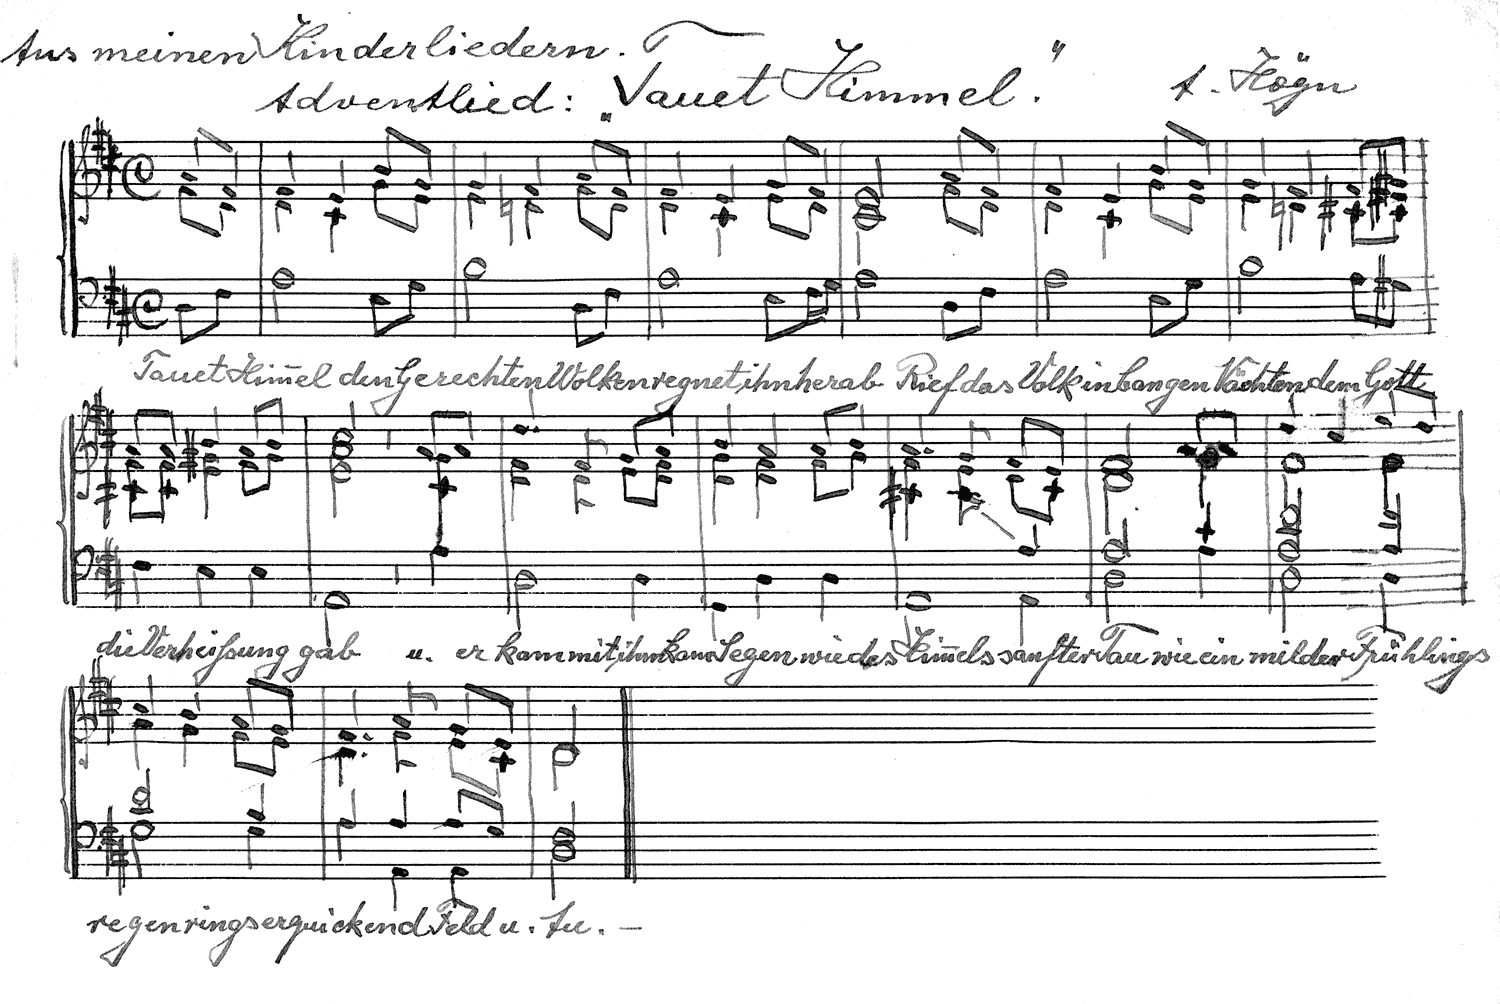
\includegraphics[width=8.373cm,height=5.604cm]{pictures/zulassungsarbeit-img033.png}

Arrangement des Liedes „Tauet Himmel“
von August Högn für den Schuleinsatz\\
\end{supertabular}
\end{flushleft}
\end{minipage}
\end{center}

\subsection{Högn und der Nationalsozialismus}

Aus
den Jahren 1936 und 1937 sind Dokumente erhalten, in denen August Högn
in der Funktion des Beauftragten für {\textquotedbl}Schutz des
Volksguts{\textquotedbl}, \footnote{Dokument Nr. 162, Brief von Albert
Schroll, Gemeindesekretär an August Högn, 21.1.1937}
Untergruppenführers \footnote{Dokument Nr. 128, Einteilung der
Gemeindegruppe Viechtach, 5.7.1937} und
Gemeindegruppenführers \footnote{Dokument Nr. 130, Brief von
Gemeindegruppenführer August Högn an alle Block- u. Hauswarte,
23.10.1936} hervortritt. Mit „Schutz des Volksguts“ wurden zur NS-Zeit
Metallsammlungen bezeichnet, an die sich auch die Schulen
beteiligten. \footnote{Interview Nr. 17, Max Holler, 26.8.2004, Absatz
16} Aus einem Dokument geht hervor, dass Högn als Führer der
Untergruppe Ruhmannsfelden der Gemeindegruppe Viechtach vier Blockwarte
unter sich hatte. \footnote{Dokument Nr. 128, Einteilung der
Gemeindegruppe Viechtach, 5.7.1937} In einem anderen Dokument
unterzeichnete der Gemeindegruppenführer Högn, wohl synonym gebraucht
zu Untergruppenführer, eine Einladung an alle Haus- und Blockwarte zur
Schulung im Luftschutz. Aufgrund der unvorstellbaren Verbrechen des
NS-Regimes sind Fragen nach der Zusammenarbeit des Einzelnen mit dem
damaligen Regime natürlich auch 60 Jahre nach Ende des 2. Weltkrieges
zu Recht von großer Brisanz. Doch sei vor voreiliger Vorverurteilungen
gewarnt, denn die wenigsten heute in der demokratischen Bundesrepublik
Deutschland lebenden Menschen haben diese totalitäre Diktatur mit ihren
indoktrinären Mechanismen bewusst miterlebt. Auch anhand einer noch so
drückend erscheinenden Beweislast, kann man letztlich doch nicht in
jemanden „hineinschauen“ und feststellen, ob stark das Engagement des
Einzelnen für den NS-Staat tatsächlich aus innerster Überzeugung
erfolgte. Anhand der im Folgenden geschilderten Fakten soll sich
deshalb jeder für sich selbst ein Bild von August Högn Einstellungs zur
Politik im 3. Reich machen.

Die Bewunderung, die Högn für seinen Schwiegersohn Dr. Karl
Schlumprecht, besonders für dessen politische Karriere zeigte\footnote{
Interview Nr. 20, Gertraud von Molo, 23.11.2004, Absatz 34} und das
gute Verhältnis zu ihm, \footnote{Interview Nr. 2, Barbara Essigmann,
27.12.2002, Absatz 66} sind Indizien dafür, dass Högn die Ideologie des
Nationalsozialismus nicht von Grund auf ablehnt hat. Dr. Karl
Schlumprecht war nach der Machtübernahme der NSDAP erster
nationalsozialistischer Oberbürgermeister von Bayreuth bis April
1937. \footnote{http://www.bnbt.de/\~{}tr1035/bt/wer/index.htm} Später
war er als Ministerialdirektor im Finanzministerium in München
tätig \footnote{Dokument Nr. 99, Brief von Bürgermeister Sturm an Dr.
Karl Schlumprecht, 1.9.1938} und stieg sogar zum Wirtschaftminister von
Bayern auf (16.7.1943 – 21.4.1944).\footnote{
http://www.stmwivt.bayern.de/das\_ministerium/geschichte\_staatsministerium.html}
Vor allem der berufliche Werdegang Schlumprechts war der Grund, weshalb
Högn auf seinen Schwiegersohn so stolz war. Er wäre es sicherlich nicht
gewesen, hätte er die NS-Ideologie in den Grundzügen ablehnt.

\begin{center}
\begin{minipage}{6.969cm}
\begin{flushleft}
\tablefirsthead{}
\tablehead{}
\tabletail{}
\tablelasttail{}
\begin{supertabular}{m{6.769cm}}

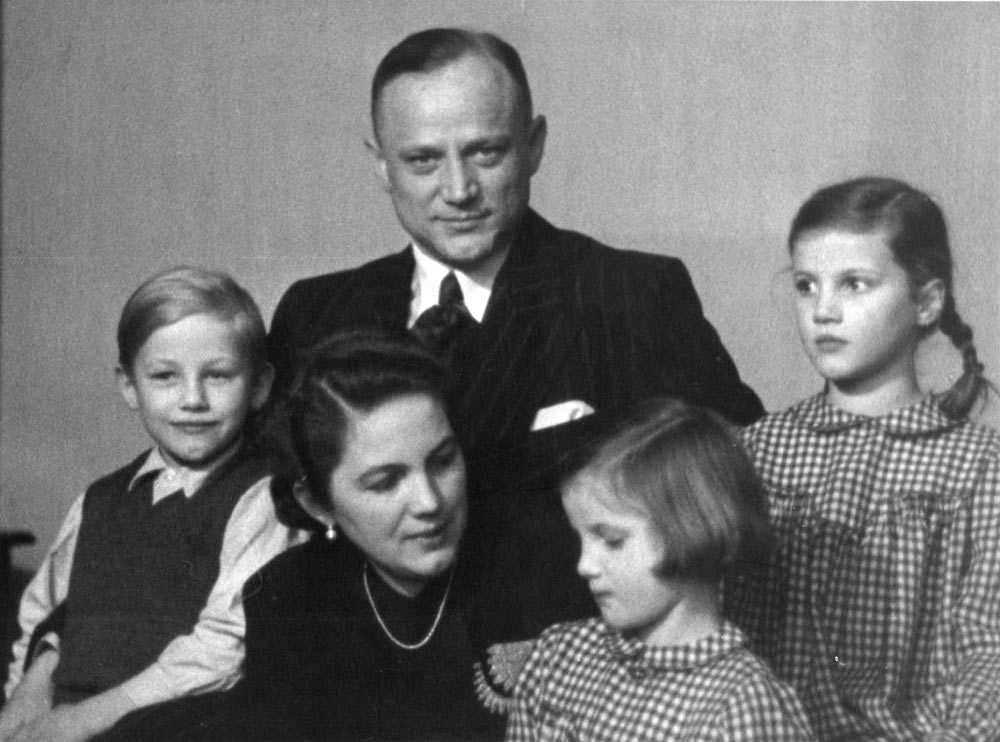
\includegraphics[width=6.588cm,height=4.888cm]{pictures/zulassungsarbeit-img034.jpg}

Dr. Karl Schlumprecht mit seiner Frau,
der Högn Tochter Frieda, und den Kindern Werner, Gertraud und Lilo\\
\end{supertabular}
\end{flushleft}
\end{minipage}
\end{center}
Högn wusste den guten Draht zu einem hohen NS-Funktionär zu nutzen –
nicht zum eigenen Vorteil, sondern zu dem der Allgemeinheit. Der
damalige Ruhmannsfeldener Bürgermeister Sturm stellte am 1. September
1938 an den Ministerialdirektor Schlumprecht im Finanzministerium einen
Antrag auf Unterstützung bei der Finanzierung des Außenputzes der
Ruhmannsfeldener Turnhalle. Der Vermerk auf dem Brief „In Abdruck an H.
Oberlehrer Högn, hier zur Kenntnis“ zeigt eindeutig, dass diese
Petition durch Högn, den ehemaligen Turnvereinsvorstand und
Veranstalter von Benefizkonzerten zugunsten der Errichtung der
Turnhalle, eingefädelt worden war. \footnote{Dokument Nr. 99, Brief von
Bürgermeister Sturm an Dr. Karl Schlumprecht, 1.9.1938}

Der Tatsache, dass Högn alle 12 Jahre des „1000-jährigen Reichs“
Schulleiter geblieben war, sagt zumindest aus, dass er den
Regimeführenden nicht negativ aufgefallen war. Seine Ernennung 1940 zum
Rektor der Volksschule zeigte, dass er zumindest auf der vorgegeben
Linie blieb. \footnote{Dokument Nr. 48, Zeitungsartikel aus Viechtacher
Bayerwald-Bote, 2.8.1958}

Eine Komposition mit eindeutig nationalsozialistischem Text lässt sicher
Rückschlüsse auf August Högns Gesinnung im 3. Reich zu. Auf den
Rückseiten der Notenblätter des Arrangements „Näher mein Gott zu dir!“
ist ein „Weihegesang“ zu finden. Auf jedem Notenblatt des Weihegesangs
steht „A. Högn“, wie bei allen August Högn eindeutig zugeordneten
Kompositionen. Högn hatte den Weihegesang nur durchgestrichen und das
Notenpapier weiter verwendet. Dieses Notenpapier war im Notenschrank
der Pfarrkirche St. Laurentius in Ruhmannsfelden aufzufinden. Hat
dieses der Komposition Högns zu Grunde liegende Gedicht – sein
Verfasser ist ungekannt – in der ersten Strophe noch Ähnlichkeit mit
Högns geistlicher Komposition, dem „Grablied für die auf dem Felde der
Ehre Gefallen op. 35“, so wird spätestens in der dritten Strophe klar,
wenn von „Steigt ein, der aus Walhallas Höhe, hoch ist es Zeit zur Tat“
die Rede ist und damit wohl die „Vorsehung“ Hitlers gemeint ist, dass
es sich nicht nur um einen patriotischen, sondern
nationalsozialistischen Text handelt. Der Weihegesang wurde mit
Sicherheit einige Male bei der weltlichen Trauerfeier für gefallene
Soldaten aufgeführt, die vor dem kirchlichem Requiem
stattfand, \footnote{Interview Nr. 6, Wilhelm Ederer, 2.1.2003, Absatz
6} da die mit Tinte geschriebenen Stimmen Flecken aufweisen, wie sie
nur Regentropfen verursachen können. Besonders irritiert, dass der
Weihegesang sowohl stilistisch als auch bezüglich der Besetzung, kaum
einen Unterschied zu den von Högn komponierten christlichen Grabliedern
ausmacht (siehe  „Weihegesang Es-Dur“, Seite
). Wie August Högn selbst zum Inhalt dieses
Texts stand, den er vertont hat, wird wohl unbekannt bleiben. Man kann
davon ausgehen, dass von der nationalsozialistischen Partei an ihn
Anfragen erfolgten, nicht nur die Gestaltung der geistlichen, sondern
auch der weltlichen Trauerfeier zu übernehmen. Wie er es in allen
anderen musikalischen Feldern gewohnt war, griff Högn auch hier zur
Feder, um passende Musik zu dem passenden Text zu schreiben. Doch
ernsthafte Konsequenzen wären sicher ausgeblieben, wenn er die Bitten
ausgeschlagen und schon gar nicht, wenn er ein Werk eines anderen
Komponisten aufgeführt hätte.

\begin{center}
\begin{minipage}{8.835cm}
\begin{center}
\tablefirsthead{}
\tablehead{}
\tabletail{}
\tablelasttail{}
\begin{supertabular}{m{8.635cm}}

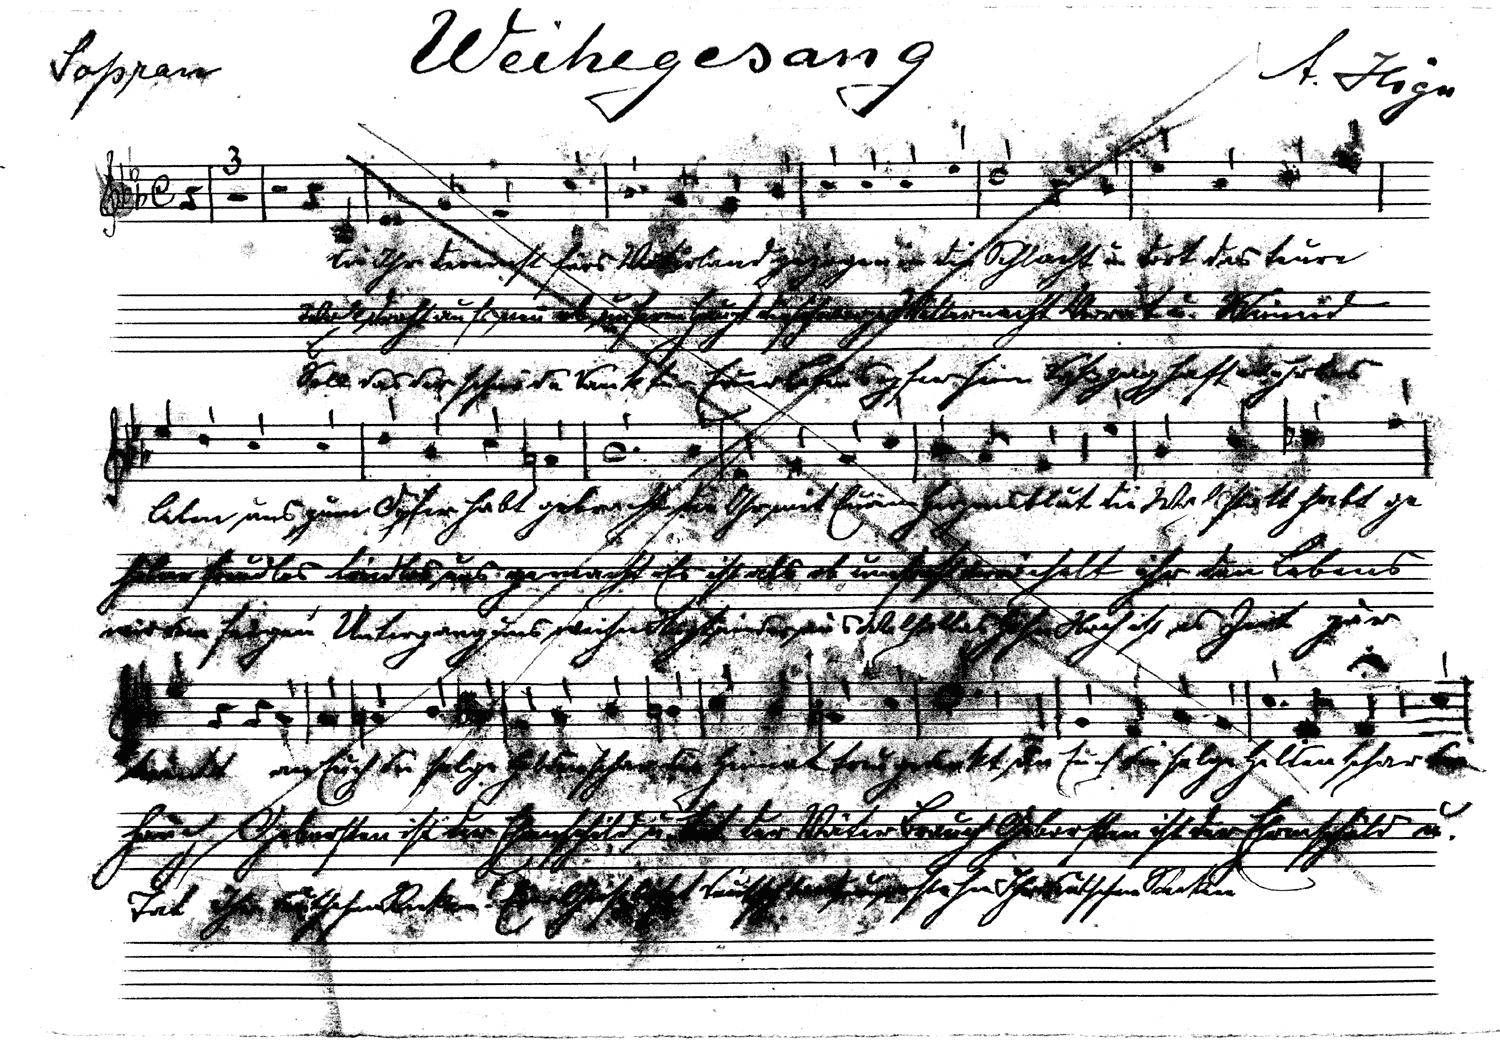
\includegraphics[width=8.453cm,height=5.678cm]{pictures/zulassungsarbeit-img035.png}

Sopran-Stimme des Weihegesang Es-Dur\\
\end{supertabular}
\end{center}
\end{minipage}
\end{center}
Als treuer Parteianhänger ist August Högn jedoch keinem der sechs zu
diesem Thema befragten Zeitzeugen in Erinnerung geblieben.\footnote{
Interview Nr. 4, Maria Schröck, 30.12.2002, Absatz 24; Interview Nr. 6,
Wilhelm Ederer, 2.1.2003, Absatz 24 – 26; Interview Nr. 16, Maria
Freisinger, 25.8.2004, Absatz 40; Interview Nr. 17, Max Holler,
26.8.2004, Absatz 18; Interview Nr. 24, Johann Glasschröder,
28.12.2004, Absatz 18; Interview Nr. 26, Eva Ertl, 9.2.2005, Absatz 28}
Als fanatische Anhängering der NS-Ideologie prägten sich einige der
Befragten stattdessen die seit 1942 \footnote{Reicheneder-Chronik,
Schulwesen, Blatt 112 Rückseite} an der Volksschule Ruhmannsfelden
unterrichtende Lehrerin Charlotte Werner ein. In ihrem Unterricht
musste Schüler aus einem Kalender Vorträge über herausragende
Persönlichkeiten des NS-Regimes halten. Vergleichbares ist aus Högns
Unterricht nicht bekannt. \footnote{Interview Nr. 6, Wilhelm Ederer,
2.1.2003, Absatz 24 – 28}

Rückschlüsse auf Högns Einstellung zu Hitlers Politik lassen sich nicht
zuletzt aus seinem in der Nachkriegszeit entstandenen Geschichtswerk
lesen. Folgende Textpassage aus der „Geschichte von Zachenberg“ lässt
sogar einen Interpretationsspielraum offen im Bezug auf seine anfangs
positive Einstellung zur NS-Ideologie, die sich im Lauf der Zeit hin
zur Ablehnung verändert haben könnte: \textit{„Die 1932/33
hereinbrechende Hitlerzeit hat zwar auf der einen Seite dieser
schlimmen Arbeitslosigkeit ein Ende gesetzt, aber auf der anderen Seite
den unheilvollen zweiten Weltkrieg heraufbeschworen, der das größte
Unglück, das je über ein Land und seine Bevölkerung kommen konnte, in
übervollem Maße über Deutschland ausgeschüttet hat.“ } \footnote{Högn,
Zachenberger, Blatt 17 (erster Teil)}\textit{ }Als ob er sich selbst
für seine anfängliche Gefolgschaft Hitlers rechtfertigen will, führt er
die Bekämpfung der Arbeitslosigkeit durch Hitler als eine zu würdigende
Errungenschaft an, geht aber sehr deutlich auf Distanz zur späteren
NS-Politik, die die „Kriegsfurie“, \footnote{Högn, Ruhmannsfelden,
Seite 16} – so nennt er den 2. Weltkrieg in der „Geschichte von
Ruhmannsfelden“ – verursacht hat, als er vollständig dessen Folgen
aufzählt. Wie ein Läuterungsversuch erscheinen die ausgedehnten
Passagen in seiner „Geschichte von Ruhmannsfelden,“ in denen er den
beiden Ruhmannsfeldener Widerständlern, Bürgermeister Sturm und
Studienrat Leonhard Donauer, die nur mit viel Glück der Exekution durch
die SS entronnen waren, ein Denkmal setzt. \footnote{Högn,
Ruhmannsfelden, Seite 32}

\begin{center}
\begin{minipage}{4.928cm}
\begin{flushleft}
\tablefirsthead{}
\tablehead{}
\tabletail{}
\tablelasttail{}
\begin{supertabular}{m{4.728cm}}

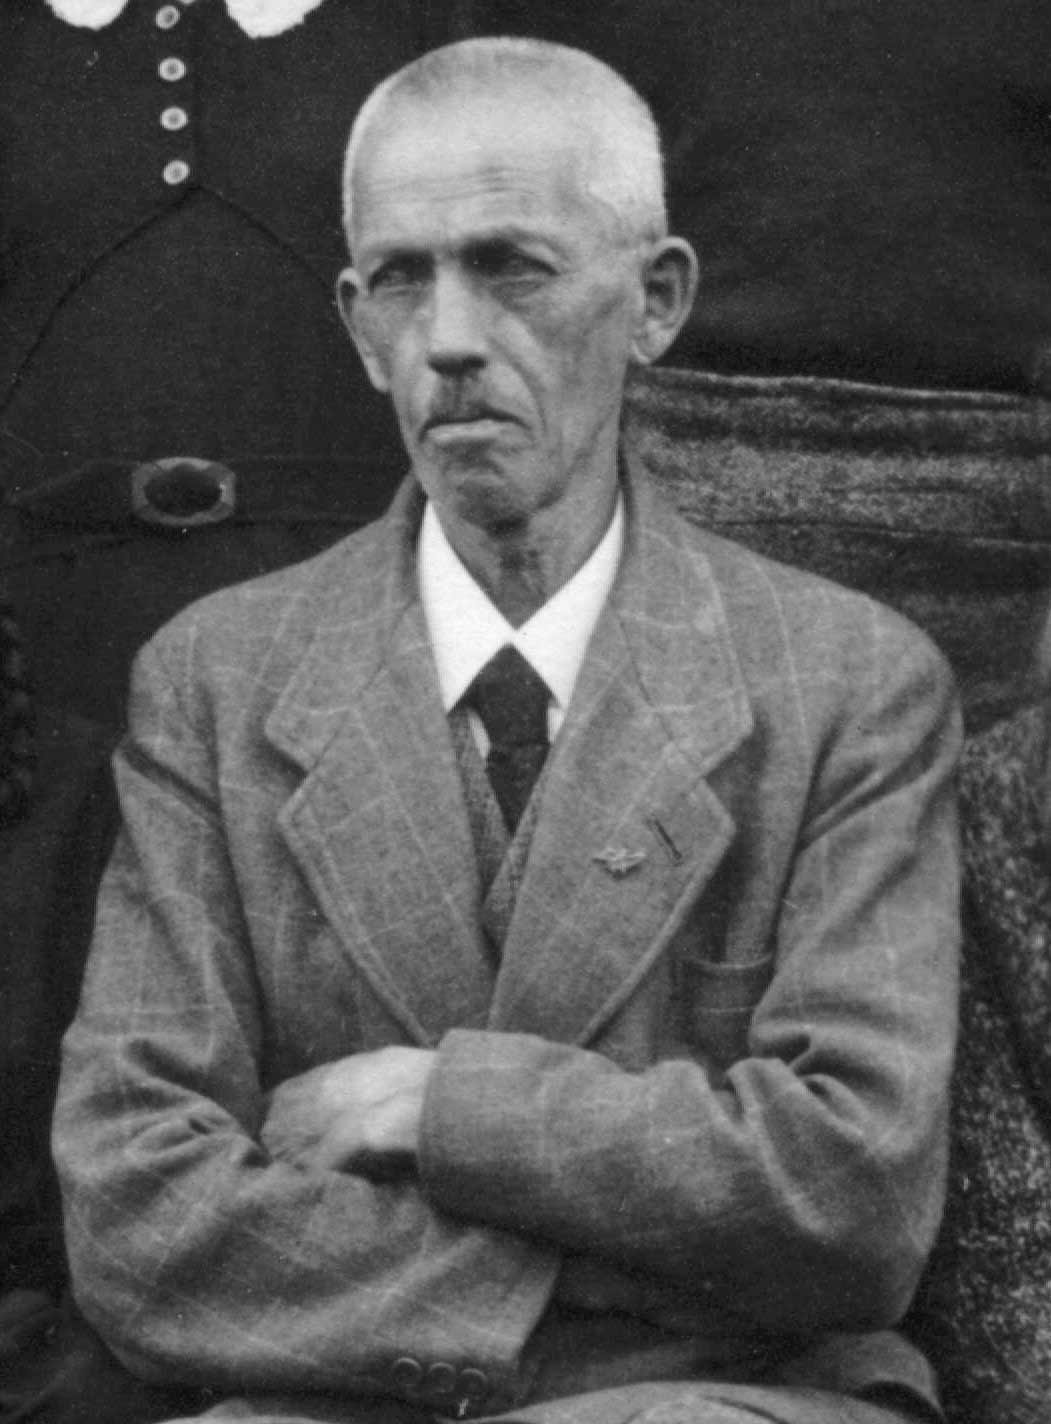
\includegraphics[width=4.503cm,height=6.103cm]{pictures/zulassungsarbeit-img036.jpg}

August Högn 1944: Das Bild eines eher
im inneren Konflikt lebenden, gebrochenen Mannes als das eines stolzen,
überzeugten Nazis.\\
\end{supertabular}
\end{flushleft}
\end{minipage}
\end{center}
Außer Frage steht, dass Högn kein Rassist war. Franz Danziger,
Kirchenchorsänger, Violinist und schließlich Högns Nachfolger als
Chorregent, war ein Halbjude, wie er im Jargon der Nationalsozialisten
geheißen hätte. Er erwähnte in seinen Memoiren über Högn kein einziges
schlechtes Wort. Viel mehr ehrte er seinen ehemaligen Lehrer, indem er
einige seiner Kompositionen aufführte.

Högns Chorregententätigkeit während des Krieges ist ebenfalls ein
Anhaltspunkt dafür, dass Högn nicht in allen Bereichen im Sinne der
NS-Ideologie gehandelt hat. Ein wirklich überzeugter Anhänger der
Weltanschauung Hitlers hätte versucht Religionen eher zu bekämpfen, als
sie durch Chorleiter- und Organistendienste doch maßgeblich zu fördern.

\subsection{Chorregent in schwieriger Zeit}
\hypertarget{RefHeadingToc100333735}{}Am 25.1.1940 starb der erst 36
Jahre alte Chorregent und Gemeindesekretär Albert Schroll, der 10 Jahre
lang in Ruhmannsfelden wirkte. \footnote{Korrespondenz Nr. 90, Brief
von Pfarramt Kollnburg an Josef Friedrich, 13.1.2005} Er erkrankte
schon 1939, sodass der Lehrer Ertl für Schroll als Klavierbegleiter bei
einem Singspiel einspringen musste. \footnote{Interview Nr. 16, Maria
Freisinger, 25.8.2004; Absatz 44} August Högn vertrat Schroll als
Chorregent und Organist während seiner Krankheit und nach dessen Tod
übernahm er seine Stelle \footnote{Interview Nr. 2, Barbara Essigmann,
27.12.2002, Absatz 6} aushilfsweise, wie es den Chorabrechnungen zu
entnehmen ist. \footnote{Dokument Nr. 136, Chorabrechnung Beerdigungen
und Trauungen, 3. Quartal 1952; Dokument Nr. 137, Chorabrechnung Ämter
und Messen, 3. Quartal 1952} Der 61-jährige und daher nicht mehr
wehrfähige Högn blieb aber Chorregent und Organist während des gesamten
2. Weltkriegs, da aufgrund der Kriegssituation kein hauptamtlicher
Kirchenmusiker als Nachfolger für Schroll verfügbar war. Nach dem Krieg
wurde Högn infolge der Entnazifizierung vom Schuldienst suspendiert und
dann in den Ruhestand versetzt, sodass der Weiterführung der
Chorregententätigkeit durch Högn in Form der Unvereinbarkeit von Schul-
und Kirchendienst nichts mehr im Wege stand. Zu Beginn von Högns
dritter Chorregentenzeit kehrte man gezwungenermaßen zur gewohnten
Praxis zurück, bei Beerdigungen den Unterricht ausfallen zu
lassen. \footnote{Interview Nr. 16, Maria Freisinger, 25.8.2004, Absatz
6; Interview Nr. 6, Wilhelm Ederer, 2.1.2003, Absatz 6} Diese in der
Weimarer Republik geduldete Regelung wurde von den Behörden des
religionsfeindlichen NS-Regimes bald unterbunden. Josef Brunner – er
war zu jung für den Kriegseinsatz \footnote{Interview Nr. 8, Josef
Brunner, 3.1.2003, Absatz 2} – und eine Mallersdorfer Schwester, die an
der Kinderbewahranstalt arbeitete, übernahmen deshalb den
Organistendienst bei Beerdigungen an Stelle von August Högn.\footnote{
Interview Nr. 16, Maria Freisinger, 25.8.2004, Absatz 6}

\begin{center}
\begin{minipage}{5.593cm}
\begin{flushleft}
\tablefirsthead{}
\tablehead{}
\tabletail{}
\tablelasttail{}
\begin{supertabular}{m{5.393cm}}

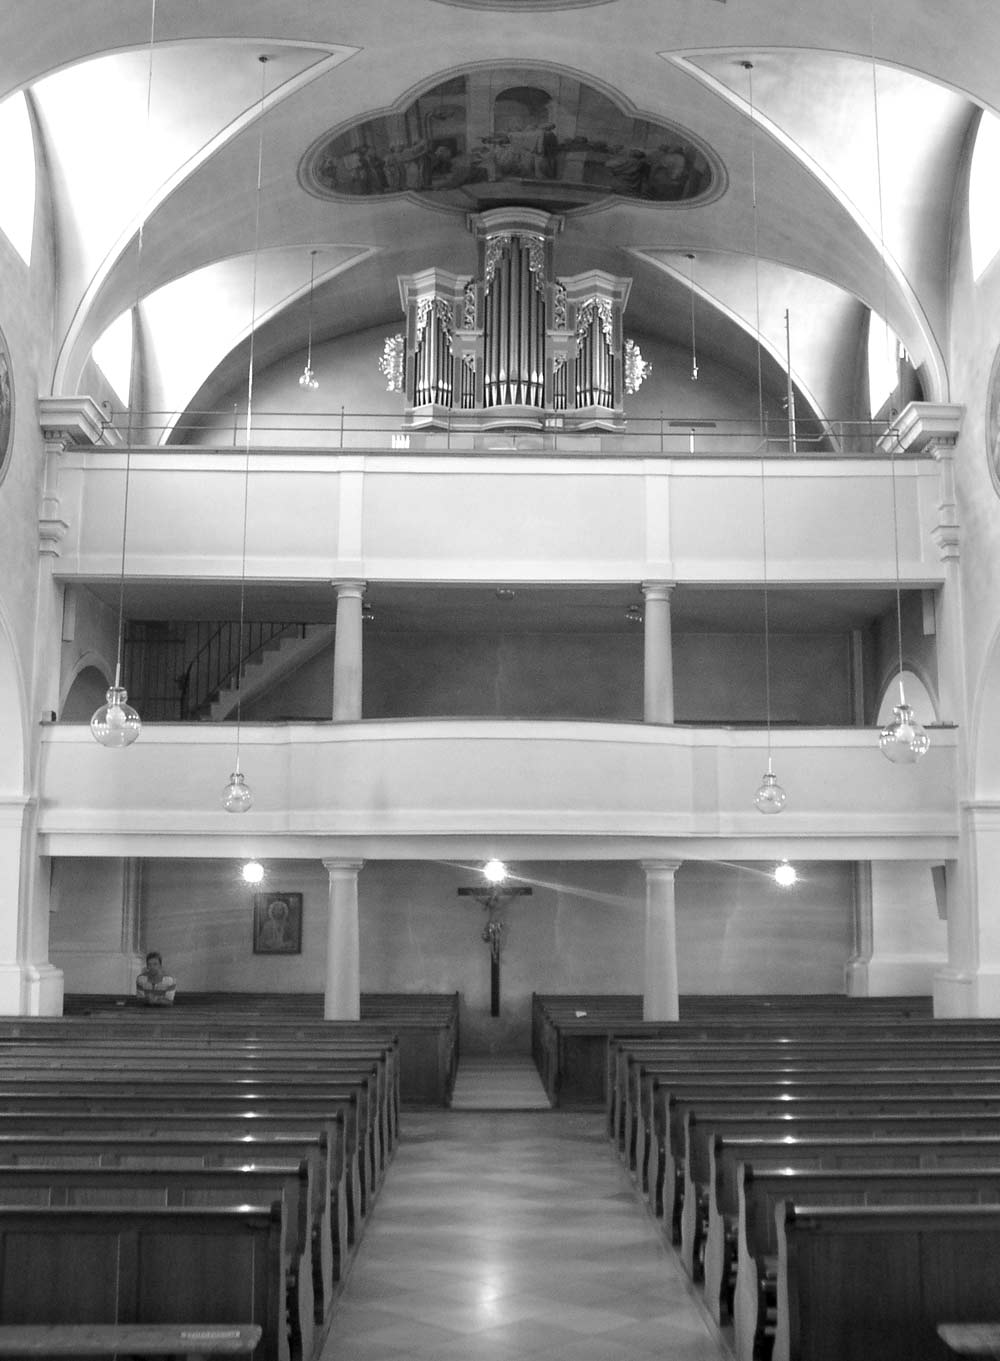
\includegraphics[width=5.001cm,height=6.805cm]{pictures/zulassungsarbeit-img037.jpg}

Pfarrkirche St. Laurentius
Ruhmannsfelden, Blick zur Orgelempore\\
\end{supertabular}
\end{flushleft}
\end{minipage}
\end{center}
Högns 3. Dienstzeit als Chorregent durchlief eine der schlimmsten Phasen
– nicht nur für die Kirchenmusik: Die Zeit des 2. Weltkriegs. Schon
1939 wurden vier Lehrer, die im Orchester mitwirkten,\footnote{
Interview Nr. 2, Barbara Essigmann, 27.12.2002, Absatz 4} zum
Kriegsdienst eingezogen. \footnote{Reicheneder-Chronik, Schulwesen,
Blatt 112 Vorder- und Rückseite} Einheimische Musiker des Orchesters,
wie Lorenz Schlagintweit, blieben von einem Kriegseinsatz genauso wenig
verschont. \footnote{Interview Nr. 13, Lorenz Schlagintweit,
29.11.2003, Absatz 2} Große Aufführungen mit Orchester an Festtagen,
wie von mehreren Zeitzeugen berichtet, \footnote{Interview Nr. 12,
Emilie Seidl, 23.4.2003, Absatz 14} dürften daher eher vor Ausbruch des
2. Weltkriegs, also zur Zeit von Chorregent Schroll, stattgefunden
haben. Besonders für das Streichorchester stellte der Krieg einen Bruch
dar. Als Ersatz etablierte sich eine Blechbläserformation, die sich aus
älteren Musikern der umliegenden Blaskapellen zusammensetzte. Die
Männerstimmen des Kirchenchores waren den Umständen entsprechend mit
nur zwei Sängern, nämlich Schwannberger und Holzfurtner, dünn
besetzt. \footnote{Interview Nr. 16, Maria Freisinger, 25.8.2004,
Absatz 6} Auch von der Orgel der Ruhmannsfeldener Pfarrkirche forderte
der Krieg seinen Tribut. Angesichts des geringen Metallgewinns, den die
am 12.6.1944 zum Ausbau bestimmten dünnwandigen Pfeifen und Leitungen
erbrachten, wird einerseits die aussichtslose Lage der
Kriegswirtschaft, andererseits die bewusste Schikane der Nazis
gegenüber der Kirche deutlich. Die Orgel – ihr fehlten die Register
Quintatön, Vox coelestis des ersten und alle metallischen Pfeifen
einschließlich der Windleitungen des zweiten Manuals\footnote{
Reicheneder-Chronik, Orgel, Blatt 74 Rückseite} – erlitt in der
Nachkriegszeit durch eine lange Trockenheit zusätzlichen großen
Schaden, ehe die Orgel 1947 vom Orgelbaumeister Kratochwill aus
Plattling restauriert wurde. \footnote{Högn, Ruhmannsfelden, S. 29}

Ob Högns Probenpraxis – die Proben fanden in seiner Wohnung
statt \footnote{Interview Nr. 2, Barbara Essigmann, 27.12.2002, Absatz
32} – eine Anpassung an den durch den Krieg geschmälerte Chor war oder
ob der Probenort auch schon in seiner ersten und zweiten
Chorregentenzeit derselbe war, kann aus Mangel an Zeitzeugen der
früheren Chorregentenzeiten nicht geklärt werden. Die Probenarbeit in
seiner Dienstwohnung hatte für Högn im allgemeinem einige praktische
Vorteile, und zwar aus folgenden Gründen: Hätte der Chor in der Kirche
geprobt, wäre es vor allem im Winter besonders kalt gewesen, da auf der
Orgelempore ein Fenster undicht war. \footnote{Interview Nr. 5, Barbara
Essigmann, 2.1.2003, Absatz 26} Einen beheizten Proberaum konnte die
Pfarrgemeinde damals nicht zu Verfügung stellen, sodass Högns große
Lehrerwohnung willkommene Alternative zur Kirche war. Außerdem besaß
Högn keinen Kirchenschlüssel, sodass er dem Mesner hätte Bescheid geben
müssen, damit die Kirche abends offen blieb. Nach der Probe hätte Högn
den Schlüssel im Pfarrhof zurückgeben müssen, was an sich relativ
umständlich gewesen wäre. \footnote{Interview Nr. 2, Barbara Essigmann,
27.12.2002, Absatz 88} Einige Zeitzeugen behaupten, dass nicht nur eine
einzige Stimmgruppe \footnote{Interview Nr. 2, Barbara Essigmann,
27.12.2002, Absatz 34} oder der komplette Chor in seiner Wohnung
probte, sondern auch das Blechbläserquartett. Nur die Generalprobe fand
in der Kirche statt. \footnote{Interview Nr. 13, Lorenz Schlagintweit,
29.11.2003, Absatz 4} Die Proben wurden auch nicht regelmäßig
abgehalten, beispielsweise jede Woche an einem bestimmten Wochentag,
sondern fanden nur dann statt, wenn ein neues Repertoire für große
Festtage erarbeitet werden musste. \footnote{Interview Nr. 2, Barbara
Essigmann, 27.12.2002, Absatz 48} Eine regelmäßige Probenarbeit machte
anscheinend wenig Sinn, wenn man sich den täglichen Einsatz der
Hauptsänger und –sängerinnen an den Gottesdiensten vergegenwärtig.
Durch die vielen Aufführungen hatte der Chor Routine und manche
Probearbeit wurde nach den Gottesdiensten geleistet.\footnote{
Interview Nr. 5, Barbara Essigmann, 2.1.2003, Absatz 36}

Vielleicht ist es aber auch auf die Proben in der privaten Wohnung
zurückzuführen, dass die Kirchenmusik in Ruhmannsfelden dem
deutschlandweiten Kulturaufschwung nach Ende des Krieges nicht folgte,
– man denke an die vielen Kleinkunstbühnen, die aus dem Boden schossen,
oder Konzerte, die in den Ruinen der ehemaligen Konzertsäle abgehalten
wurden – sondern eher einen Niedergang erlebte. \footnote{Interview Nr.
9, Dr. Doraliesa Wiegmann, 19.1.2003, Absatz 4; Interview Nr. 24,
Johann Glasschröder, 28.12.2004, Absatz 36} Die in Högns Wohnung
abgehaltenen Proben schienen zu einer Privatveranstaltung verkommen zu
sein. Nur für die Hauptsängerinnen hielt Högn Proben nach Ende des 2.
Weltkriegs. Die Sängerin Maria Freisinger hat jahrelang sonntags an den
Gottesdiensten mitgewirkt, doch an Proben konnte sie sich nicht
erinnern. \footnote{Interview Nr. 16, Maria Freisinger, 25.8.2004,
Absatz 8} Der öffentliche Chor wurde zu einem nach außen hin
abgeschlossenen Zirkel von eng befreundeten Hauptsängerinnen, zu dem
nur schwer neue Mitglieder stoßen konnten.

\begin{center}
\begin{minipage}{3.491cm}
\begin{flushleft}
\tablefirsthead{}
\tablehead{}
\tabletail{}
\tablelasttail{}
\begin{supertabular}{m{3.291cm}}

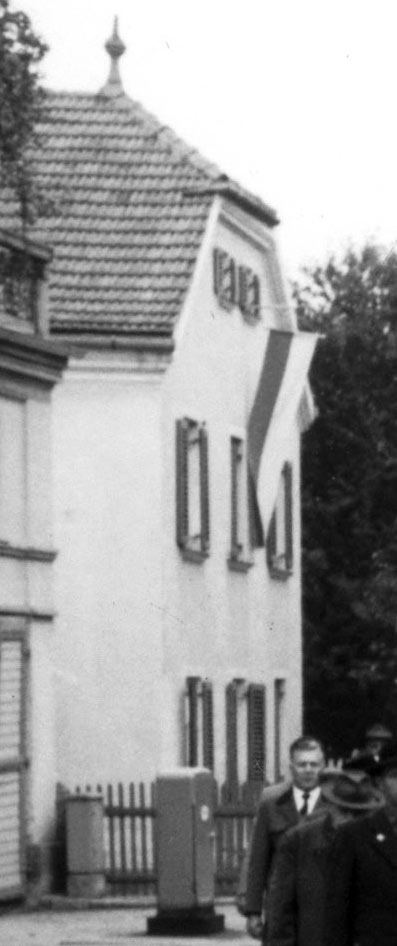
\includegraphics[width=3.108cm,height=7.408cm]{pictures/zulassungsarbeit-img038.jpg}

Im Erdgeschoss dieses Hauses wohnte
Högn ab 1945 bis zu seinem Tod\\
\end{supertabular}
\end{flushleft}
\end{minipage}
\end{center}
\begin{flushleft}
\tablefirsthead{}
\tablehead{}
\tabletail{}
\tablelasttail{}
\begin{supertabular}{m{4.6330004cm}}

\begin{center}

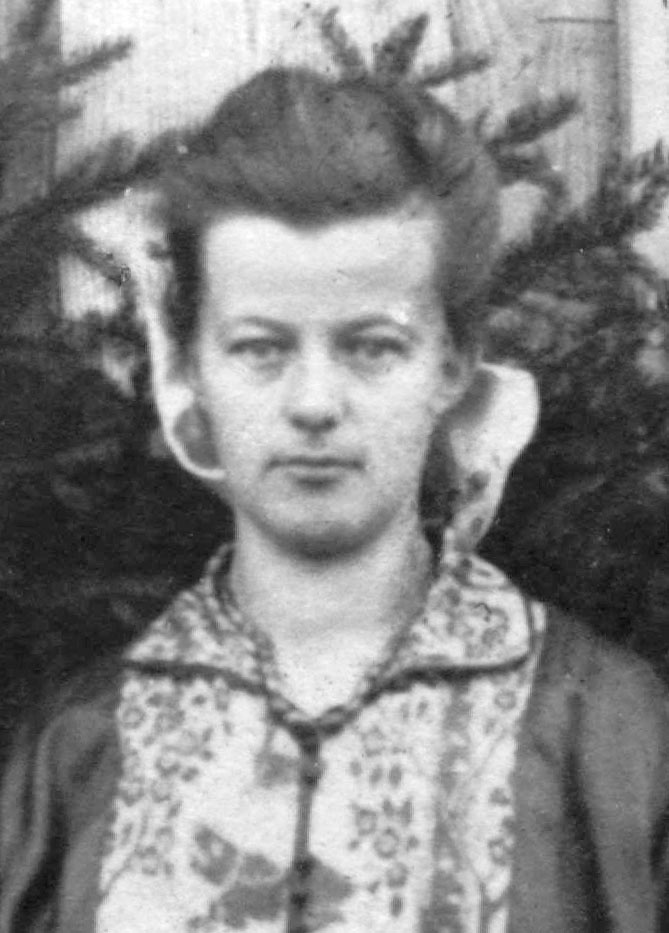
\includegraphics[width=4.3cm,height=5.973cm]{pictures/zulassungsarbeit-img039.jpg}

\end{center}
Theres Raster\\
\end{supertabular}
\end{flushleft}
Dass der Zustrom von neuen Sängerinnen und Sängern ausblieb, lag sicher
auch an dem Verhalten der Hauptsängerinnen. Sie hatten hauptsächlich
aus einem bestimmten Grund kein Interesse an einem größeren Chor:
Geld. \footnote{Interview Nr. 24, Johann Glasschröder, 28.12.2004,
Absatz 46} Denn je mehr Personen im Chor mitgesungen hätten, desto
öfter wäre die finanzielle Entschädigung, die dem Hauptchor zustand
aufzuteilen gewesen. Diese war etwa genau so hoch wie die des
Chorregenten. \footnote{Dokument Nr. 137, Chorabrechnung Ämter und
Messen, 3. Quartal 1952; Dokument Nr. 136, Chorabrechnung Beerdigungen
und Trauungen, 3. Quartal 1952; Dokument Nr. 138, Chorabrechnung, 4.
Quartal 1946} Das „Gehalt“ der einzelnen Sängerinnen wäre somit immer
kleiner ausgefallen. Aus dieser Sichtweise ist zum Beispiel das
Verhalten der Sängerin Theres Raster gegenüber neuen Chormitgliedern
durchaus nachvollziehbar. Raster war für den Notenschrank zuständig und
bestimmte sogar öfter als Högn, welches Stück gesungen werden
sollte. \footnote{Interview Nr. 2, Barbara Essigmann, 27.12.2002,
Absatz 94} Waren zu wenige Singstimmen vorhanden, und das war bei den
meist handgeschriebenen Notenmaterialien oft der Fall, gab sie
insbesondere den jungen Sängerinnen kein Notenblatt.\footnote{
Interview Nr. 16, Maria Freisinger, 25.8.2004, Absatz 8} Neue
Chormitglieder fühlten sich logischerweise weniger akzeptiert, wenn sie
wiederholt kein Notenblatt bekamen, noch dazu wenn ihnen nicht
klargemacht wurde, warum sie keine Stimmestimme bekommen
hatten. \footnote{Interview Nr. 16, Maria Freisinger, 25.8.2004, Absatz
12}

Der Hauptgrund, weshalb der Chor der Nachkriegszeit so wenige Mitglieder
zählte, ist aber in der Person von August Högn zu sehen. Mit 70 Jahren
hatte er nicht mehr den Elan, neue Sänger zu integrieren oder sich dem
intriganten Verhalten der Hauptsängerinnen entgegen zu
stellen. \footnote{Interview Nr. 16, Maria Freisinger, 25.8.2004,
Absatz 12} Vielleicht hat sich nicht nur sein hohes Alter, sondern auch
die Tatsache, dass er zeitlebens den Chorregentendienst nur
provisorisch oder aushilfsweise, paradoxerweise aber fast 20 Jahre lang
ausübte, wie in jedem Protokoll ausdrücklich erwähnt wird, und immer
nur als „Notnagel“ angesehen wurde, auf seine Einsatzbereitschaft
negativ ausgewirkt. Seinen drei großen heimatkundlichen Abhandlungen,
die alle in der Nachkriegszeit entstanden sind, entnimmt man, dass Högn
ab 1945 sein Hauptbetätigungsfeld nicht mehr in der Kirchenmusik sah.

\subsection{Heimatforschung als Betätigungsfeld im Ruhestand}

Die Heimatkunde: Ein Hobby des
Pensionisten Högn? Nach Eintritt ins Rentenalter verfasste Högn drei
Geschichten mit heimatkundlichem Inhalt. Die lockere Abfolge ihrer
Entstehung vermittelt den Eindruck, dass sie eher unter einem Zustand
der Ablenkung, des Zeitvertreibs beziehungsweise der Zerstreuung
entstanden sind. Dies trifft bei Högn nur teilweise zu. Seine
schriftstellerische Tätigkeit kann auch mit der Vollendung einer von
der Gesellschaft an die Lehrer übertragenen Aufgabe umschrieben werden.

Eine Aktion der Regierung von Niederbayern zur Zeit der Weimarer
Republik mit dem Motto \zitat{„Pflege des
Heimatgedankens“}, \footnote{Dokument Nr. 133, Regierungsblatt zur
Pflege des Heimatgedankens, 12.11.1925} hatte das Ziel, durch
Heimatkunde, den Patriotismus und das Nationalbewusstsein der Bürger zu
stärken, um damit einen Beitrag zur Lösung der nationalen Probleme zu
leisten. Ein Rundschreiben vom 12.11.1925, das auch Högn vorlag, mit
dem Betreff \zitat{„Anlegung gemeindlicher Ortsgeschichten“}
macht die Intention dieser Aktion in wenigen Sätzen deutlich:
\zitat{„Die Voraussetzung für den Aufstieg unseres Volkes aus
dem jetzigen Tiefstande ist die Rückkehr zu deutscher Einfachheit,
Zucht und Sitte. Dazu muss der Sinn für die Heimaterde geweckt“} und
\zitat{„die Liebe zum Vaterlande entzündet [...] werden. Auf
diesen }\zitat{Grundlagen baut sich neben der körperlichen
und geistigen Ertüchtigung der Jugend die Zukunft des deutschen Reiches
auf.“} Vor allem \zitat{„die Herren Lehrer [...] sollten“
}daher\zitat{ „ohne weiteres Säumen und mit allem Nachdruck
[...] die Vorbereitung für die Herstellung der
Ortsgeschichten“} \footnote{Dokument Nr. 133, Regierungsblatt zur
Pflege des Heimatgedankens, 12.11.1925} aufnehmen. Dass die
angetragenen Vorhaben eine gewisse Verbindlichkeit hatten, zeigt schon
die Aufforderung, dass \zitat{„bis zum 1. April 1928
berichtet werden wolle, [...] in welchen Gemeinden die Vorarbeiten in
Angriff genommen worden sind (Anrede des Bearbeiters).“ }\footnote{
Dokument Nr. 133, Regierungsblatt zur Pflege des Heimatgedankens,
12.11.1925} Högn hat sich tatsächlich dieser Aufgabe angenommen, wie
die vielen heimatkundlichen Zeitungsartikel zeigen, die in der Zeit von
1926 bis 1928 erschienen sind. Doch es waren nur einzelne
heimatkundliche Beiträge, die entstanden sind. Die eigentlich
geforderte komplette Ortsgeschichte blieb aus. Stand der Vollendung
dieser Aufgabe die Zeitknappheit aufgrund des Schuldienstes in Wege, so
beseitigte seine Pensionierung dieses Hindernis zur umfassenden
Ortsgeschichte. \footnote{Dokument Nr. 133, Regierungsblatt zur Pflege
des Heimatgedankens, 12.11.1925} Bei der Geschichte von Zachenberg
etwa, gibt es ganz konkrete Anhaltspunkte, wonach die Initiative zur
Inangriffnahme der Arbeit nicht von Högn selbst aus ging, für den
Begriff Hobby ein notwendiges Merkmal, sondern eine an ihn
herangetragene Bitte den Grund für die Entstehung der Geschichte
lieferte.

\begin{flushleft}
\tablefirsthead{}
\tablehead{}
\tabletail{}
\tablelasttail{}
\begin{supertabular}{m{5.2310004cm}}

\begin{center}

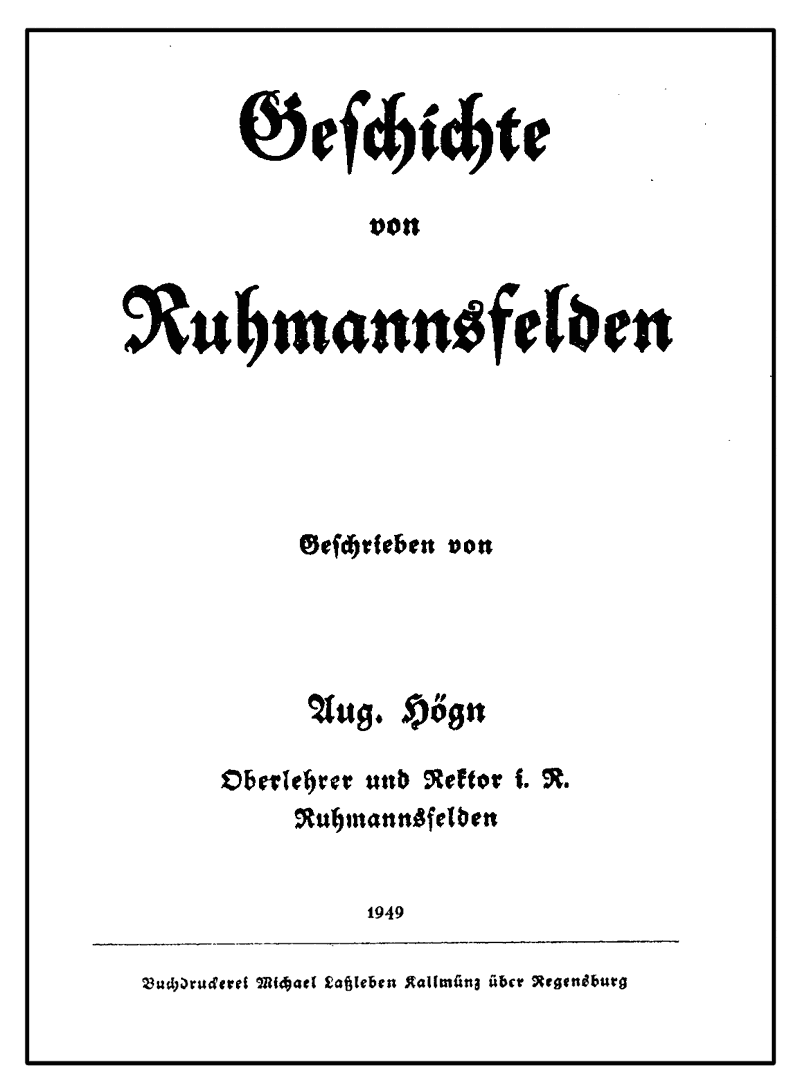
\includegraphics[width=4.995cm,height=6.833cm]{pictures/zulassungsarbeit-img040.png}

\end{center}
erste Seite der Geschichte von
Ruhmannsfelden\\
\end{supertabular}
\end{flushleft}

\begin{figure}
\img{}
\caption{}
\end{figure}

Gerade mal zwei Jahre nach Högns endgültiger Pensionierung,\footnote{
Dokument Nr. 48, Zeitungsartikel aus Viechtacher Bayerwald-Bote,
2.8.1958} erschien 1949 die „Geschichte von Ruhmannsfelden.“ Dem
rüstigen Rentner musste es eher leicht gefallen sein, Material für
seine Arbeit zu finden, konnte er doch auf eine rege Forschertätigkeit
vergangener Jahrzehnte zurückblicken und brauchte die vielen bereits
existierenden Einzelbeiträge zur Heimatgeschichte nur noch in einem
Werk zusammenfassen. Die geschichtliche Entwicklung zwei wichtiger
Institutionen am Ort hatte Högn lange vor dem 2. Weltkrieg bearbeitet:
Die Entwicklung der Ruhmannsfeldener Schule war in einer Beilage zum
Deggendorfer Donauboten 1927 erschienen und anlässlich der 100-jährigen
Einweihungsfeier der Ruhmannsfeldener Pfarrkirche wurde 1928 bis 1929
in mehreren Teilen die Geschichte der Pfarrkirche St. Laurentius im
Viechtacher Tagblatt abgedruckt. Information über die Entstehung des
Namens „Ruhmannsfelden“ oder den Zeitpunkt der Marktrechtsverleihung
beinhalteten zwei Zeitungsartikel aus dem Jahre 1926 und fanden an
exponierter Stelle Eingang in die „Geschichte von Ruhmannsfelden“. Es
war August Högn, der sich zur Frage des Namensursprungs von
„Ruhmannsfelden“ schon 1922 an den Straubinger Historiker Dr. Joseph
Keim wandte \footnote{Dokument Nr. 20, Brief von Dr. Keim an August
Högn, 30.8.1922} und die noch heute gültige Erklärung gab, wonach
Ruhmannsfelden nach dem Rodungsarbeiter „Rumar“ benannt wurde. Davor
wurde der Name „Ruhmannsfelden“ etwas trivial mit „Ruht der Mann in
Felde“ erklärt. \footnote{Interview Nr. 9, Dr. Doraliesa Wiegmann,
19.1.2003, Absatz 4} Ebenso versuchte Högn sowohl in dem erwähnten
Artikel als auch in der „Geschichte von Ruhmannsfelden“ dem Mythos,
dass einst ein Schloss am Leitenberg bestand, entgegenzuwirken. Trotz
aller realisierbaren Recherchearbeiten ist es unverkennbar, dass Högn
besonders zur frühen Geschichte Ruhmannsfeldens auf sehr wenige
Informationen zurückgreifen konnte. Das einleitende Kapitel der
Geschichte von Ruhmannsfelden „Wie hat es vor seiner Entstehung
ausgesehen?“ ähnelt in seinem Aufbau mehr einem Roman als dem Beginn
einer historischen Abhandlung und entbehrt sicherlich aller
wissenschaftlichen Beweise. Wegen fehlender Dokumente musste von Namen
wie etwa „Ruhmannsfelden“ oder „Laurentius-Kirche“ auf die mögliche
geschichtliche Entwicklung geschlossen werden. Manchmal schlussfolgerte
Högn aus diesen Anhaltspunkten etwas zuviel. Es stimmt sicher, dass
alle dem hl. Laurentius geweihten Kirchen außerhalb der Ortschaften
standen, aber dass die „Laurentius“-Kirche in Ruhmannsfelden zuerst aus
Holz war, unter den Aldersbachern dann aus Stein und dass dann auch
öfter Gottesdienste stattfanden, wie in der Geschichte von
Ruhmannsfelden steht, ist wohl rein Spekulation. \footnote{Högn,
Ruhmannsfelden, Seite 10} Als Lückenfüller dürften die Kapitel über die
Namen der Ruhmannsfeldener Fluren und Gassen und eine Auflistung der
Höhenlagen mit Barometerstand der umliegenden Berge und Ortschaften
gedient haben.

Der Entstehungsgrund der „Geschichte und Chronik der freiwilligen
Feuerwehr Ruhmannsfelden“ ist eng mit dem Ende von Högns
Schriftführertätigkeit bei der Feuerwehr verbunden. Am Stefani-Tag 1950
wurde Johann Freisinger zum Schriftführer der Feuerwehr Ruhmannsfelden
gewählt und löste somit August Högn nach 40-jähriger Dienstzeit ab. Die
\zitat{„in dankbarer Erinnerung“}  \footnote{Högn,
Ruhmannsfelden, Titelblatt} der Feuerwehr gewidmete Geschichte hat Högn
geschrieben, um seine Tätigkeit als Schriftführer abzurunden und sein
in 40 Jahren gesammeltes Wissen in diese Arbeit einfließen zu lassen.
Ein passender Übergabetermin der Chronik an die Feuerwehr wäre der zur
Verabschiedung von Högn eigens veranstaltete Ehrenabend am 11. März
1951 gewesen, doch die Chronik wurde der letzten Eintragung zufolge
erst nach dem 1. April 1951 fertig geschrieben. Aber die Arbeit war zum
Ehrenabend der Feuerwehr schon versprochen und fand deswegen lobende
Erwähnung in der Abschiedesrede des Feuerwehrkommandanten.\footnote{
Dokument Nr. 110, Abschiedsrede des Feuerwehrkommandanten Johann
Linsmeier, 3.11.1951} Die fertige Chronik überreichte Högn persönlich
dann kurze Zeit später seinem Schriftführer-Nachfolger.\footnote{
Interview Nr. 14, Johann Freisinger, 29.12.2003, Absatz 16} Die
Abhandlung ist nach Jahrgängen gegliedert und lässt daher oft
Einzelfakten unverbunden nebeneinander stehen, was das Verständnis beim
Lesen erschwert. Sie ist deshalb wohl eher als eine Stoffsammlung zur
weiteren Bearbeitung anzusehen, als ein unterhaltsamer Lesestoff für
die breite Ruhmannsfeldener Bevölkerung und war sicher nie für den
Druck bestimmt. Lediglich die länger ausformulierte Gründung der
Feuerwehr und der Bericht samt Querverweisen über den sich über
längeren Zeitraum erstreckende und deshalb in mehreren Jahren
auftauchende Streit der Gemeinden Ruhmannsfelden und Zachenberg um eine
gemeinsam angeschaffte Feuerwehrspritze bleiben dem Leser in Erinnerung
und gehen nicht in der Flut von Einzelinformationen unter.

\begin{center}
\begin{minipage}{10.007cm}
\begin{flushleft}
\tablefirsthead{}
\tablehead{}
\tabletail{}
\tablelasttail{}
\begin{supertabular}{m{5.0280004cm}m{4.578cm}}

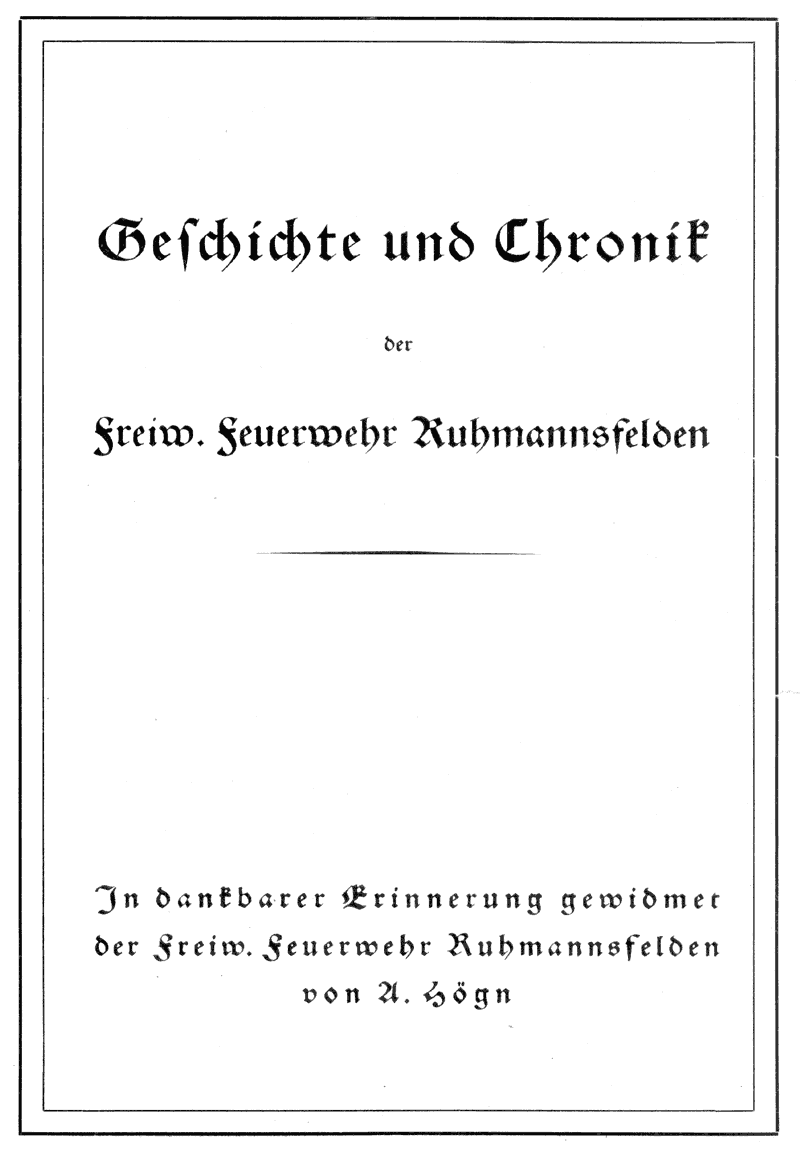
\includegraphics[width=4.847cm,height=6.997cm]{pictures/zulassungsarbeit-img041.png}

Deckblatt des Manuskripts der
„Geschichte und Chronik der Freiw. Feuerwehr Ruhmannsfelden“ &

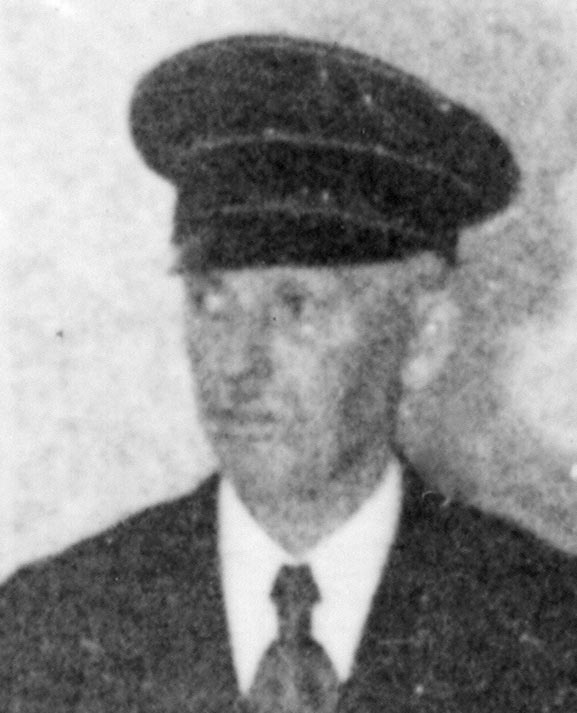
\includegraphics[width=4.396cm,height=6.997cm]{pictures/zulassungsarbeit-img042.jpg}

August Högn bei der Mitglieder-Ehrung
der Feuerwehr 1950\\
\end{supertabular}
\end{flushleft}
\end{minipage}
\end{center}

\begin{figure}
\img{}
\caption{}
\end{figure}

Ein auswärtiger, nicht in der Gemeinde Zachenberg ansässiger Bürger
lieferte die Initiative zur Entstehung von Högns „Heimat-Geschichte der
Gemeinde Zachenberg.“ Der Finanzzollrat Anton Trellinger – er war am
Landshuter Hauptstaatsarchiv als Archivpfleger angestellt – fertigte
einen 63-seitigen Akten-Auszug \footnote{Dokument Nr. 31, Brief von
August Högn an Klosterbibliothekar des Klosters Niederalteich,
26.3.1952, Dokument Nr. 33, Brief von August Högn an das Pfarramt
Grafenau, 26.3.1952} über die Gemeinde Zachenberg an. Da Trellinger die
Gemeinde Zachenberg nur flüchtig kannte und gesundheitlich sehr
angeschlagen war, \footnote{Dokument Nr. 28, Brief von Finanzzollrat
Anton Trellinger an August Högn, 25.2.1952} – er erlitt im Frühjahr
1952 einen Schlaganfall \footnote{Dokument Nr. 35, Brief von Expositus
Georg Hofmann, Schönau an August Högn, 23.10.1952} – bat er seinem
Brief die Gemeinde Zachenberg um einen ortskundigen Fachmann, der seine
Arbeit ergänzen und fortführen könnte. Den Sachbearbeitern bei der
Gemeinde dürfte es nicht schwer gefallen sein, Trellinger die
geforderte Person zu nennen: August Högn. Lange bevor Anton Trellinger
der Gemeinde Zachenberg seine Arbeit übersandte, nämlich am 25.2.1952,
und am selben Tag Högn persönlich anschrieb, \footnote{Dokument Nr. 28,
Brief von Finanzzollrat Anton Trellinger an August Högn, 25.2.1952}
hatte August Högn schon mit der Recherche begonnen und den Mettener
Benediktiner-Pater Wilhelm Fink von der beabsichtigen Geschichte von
Zachenberg in Kenntnis gesetzt und um wissenschaftliche Betreuung
gebeten. \footnote{Dokument Nr. 29, Brief von Pater Wilhelm Fink an
August Högn, 28.1.1952}

\begin{center}
\begin{minipage}{5.378cm}
\begin{flushleft}
\tablefirsthead{}
\tablehead{}
\tabletail{}
\tablelasttail{}
\begin{supertabular}{m{5.178cm}}

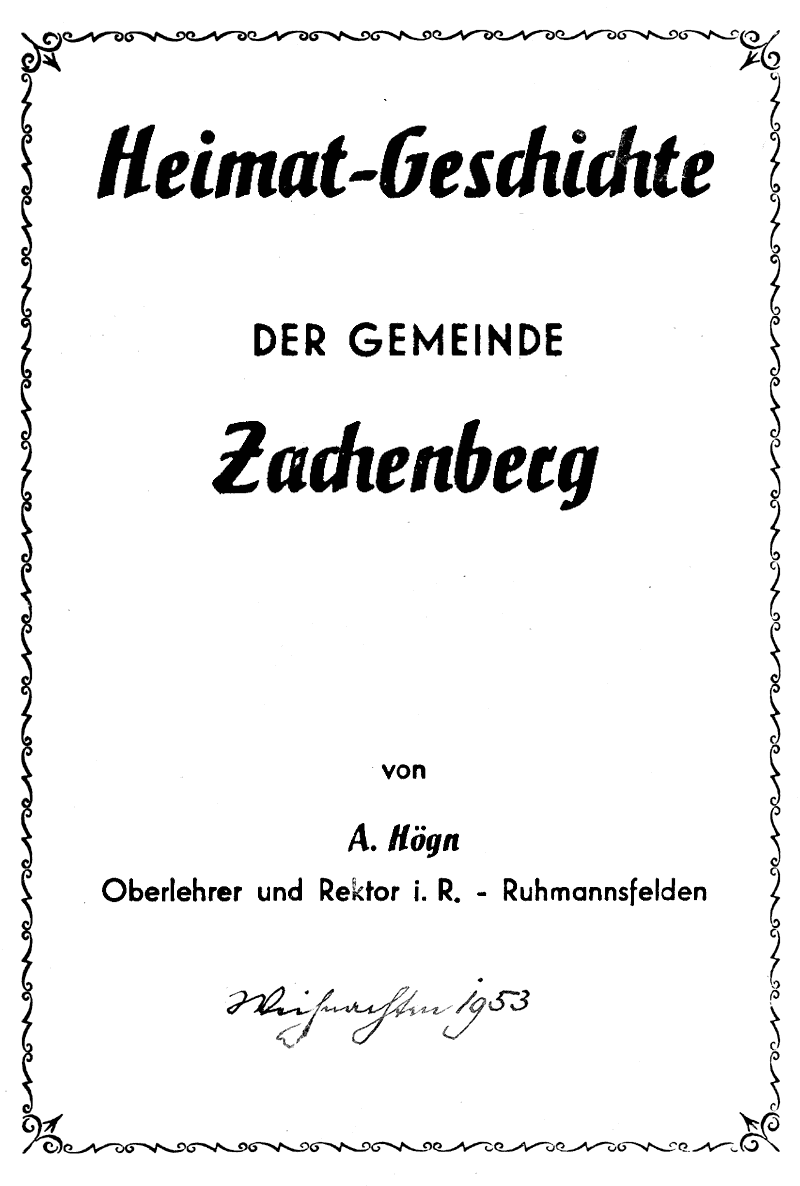
\includegraphics[width=4.995cm,height=7.405cm]{pictures/zulassungsarbeit-img043.png}

Deckblatt des Manuskripts der
„Heimat-Geschichte der Gemeinde Zachenberg“\\
\end{supertabular}
\end{flushleft}
\end{minipage}
\end{center}
Trellinger lieferte mit seinen Archivauszügen nicht nur einen wichtigen
Grundstock für Högns „Heimat-Geschichte der Gemeinde Zachenberg“,
sondern er gab ihm auch einige Tipps und Literaturhinweise.\footnote{
Dokument Nr. 28, Brief von Finanzzollrat Anton Trellinger an August
Högn, 25.2.1952} Nach fast 2-jähriger Arbeitszeit wurde die „Geschichte
von Zachenberg“ an Weihnachten 1953 fertig gestellt \footnote{Högn,
Zachenberg, Deckblatt} und an Wilhelm Fink zum Korrekturlesen
übersandt. Fink hatte besonders zum 1. Teil der Abhandlung einige
Änderungsvorschläge anzubieten. Es ist deshalb nicht verwunderlich,
dass sich die ersten Teile der „Geschichte von Ruhmannsfelden“ und der
„Geschichte von Zachenberg“ im Aufbau und in der Darstellung ziemlich
stark unterscheiden, obwohl beide Teile die geschichtliche Entwicklung
von den Anfängen der beiden benachbarten und sich unter den gleichen
Herrschaftsverhältnissen entwickelnden Gemeinden zum Thema haben. Fink
hat offensichtlich die „Geschichte von Ruhmannsfelden“ nicht Korrektur
gelesen. Im von Fink als druckreif befunden 2. Teil der Geschichte von
Zachenberg geht Högn auf die 15 Dörfer, 13 Weiler und 10 Einöde, also
auf die insgesamt 38 Ortschaften der Gemeinde Zachenberg im Einzelnen
ein.

Die Kapitel über die einzelnen Ortschaften ähneln mehr genealogischen
Studien als historischen Abhandlungen. Manchmal lassen sich aus diesen
Kapiteln Stammbäume einzelner Bauernfamilien über Jahrhunderte hinweg
ablesen. Meistens jedoch konnten die Angaben aus den sehr alten
Aktenauszügen Trellingers nicht mit den neueren Informationen aus dem
Gemeindearchiv oder von den befragten Bewohnern der jeweiligen
Ortschaft bruchlos aneinander gereiht werden. Die sehr schematische
Beschreibung der kleinsten Ortschaften selbst – sie beginnt immer mit
der Herkunfts-Erklärung des Ortsnamens und endet nach Vorstellung der
einzelnen Bauernfamilien mit Angabe der damals aktuellen Einwohner- und
Häuserzahl – wird durch Sagen und Erzählungen aufgelockert, die Högn
von älteren Bewohnern der einzelnen Orte erzählt bekam und sie in Form
von Nacherzählungen wiedergibt. Viele der von Wilhelm Fink
vorgeschlagenen Ergänzungen zum dritten, allgemeinen Teil – hier geht
es in erster Linie um die damalige aktuelle Organisation der Gemeinde –
hat Högn nicht angenommen, weil beiden Gemeinden, Zachenberg und
Ruhmannsfelden, doch sehr ähnliche Strukturen aufwiesen und er bereits
Einiges in der Geschichte von Ruhmannsfelden erwähnt hatte, wie zum
Beispiel die aus der Pfarrei hervorgegangenen Priester, die Lehrer oder
die Polizei. Deshalb erörtert er hier hauptsächlich die aktuellen
wirtschaftlichen und infrastrukturellen Aspekte der Gemeinde
Zachenberg. \footnote{Dokument Nr. 38, Brief von Pater Wilhelm Fink,
Metten an August Högn, 23.2.1954}

Als er die korrigierte Fassung der Geschichte kurz vor Ostern 1954 der
Gemeinde Zachenberg übergab, rechnete er sicher mit einer schnellen
Drucklegung seiner Arbeit, ähnlich wie bei der Geschichte von
Ruhmannsfelden, sonst hätte er sich nicht schon von der Druckerei
Michael Laßleben in Kallmünz ein Angebot geben lassen und sich sogar
schon einen Werbetext für ein Inserat oder ein Plakat
überlegt. \footnote{Dokument Nr. 39, Brief von August Högn an
Bürgermeister Ludwig Bielmeier, Zachenberg, 31.3.1954}

\begin{center}
\begin{minipage}{5.812cm}
\begin{center}
\tablefirsthead{}
\tablehead{}
\tabletail{}
\tablelasttail{}
\begin{supertabular}{m{5.612cm}}

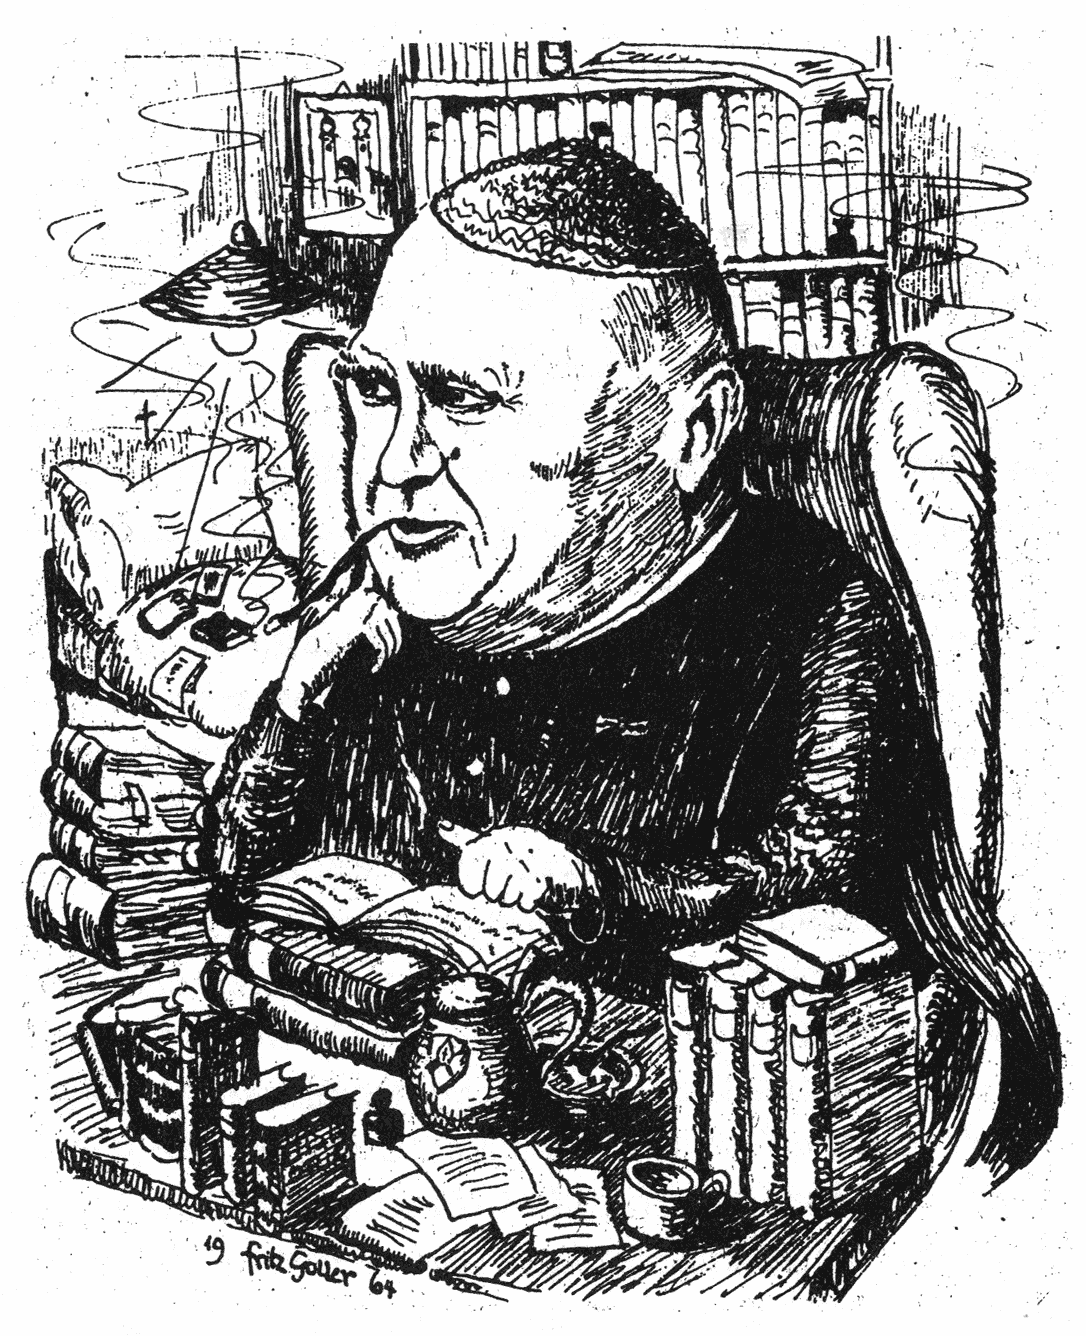
\includegraphics[width=5.429cm,height=6.68cm]{pictures/zulassungsarbeit-img044.png}

Wilhelm Fink in einer Karikatur von
Fritz Goller\\
\end{supertabular}
\end{center}
\end{minipage}
\end{center}

\begin{figure}
\img{}
\caption{}
\end{figure}

Erst am 7. Mai 1956 versicherte der Zachenberger Bürgermeister Bielmeier
August Högn, auf seine Anfrage hin, dass der Gemeinderat über die
Veröffentlichung der „Geschichte von Zachenberg“ in der nächsten
Sitzung beraten würde. \footnote{Dokument Nr. 40, Brief von
Bürgermeister Ludwig Bielmeier, Zachenberg an August Högn, 7.5.1956}
Die Gemeindevorsteher hatten wohl von Anfang an kein Interesse an einer
Drucklegung. \footnote{Interview Nr. 14, Johann Freisinger, 29.12.2003,
Absatz 13 – 14} Kein einziges Wort ist über den Druck des Buchs im
Protokoll der Gemeinderatssitzung vom 17.5.1956 zu finden. Stattdessen
wurde beschlossen, Högn zum Ehrenbürger der Gemeinde Zachenberg zu
ernennen und ihm als \zitat{„Entschädigung“ }für seine
Bemühungen ein \zitat{„Geldgeschenk im Ermessen des 1.
Bürgermeisters“} \footnote{Dokument Nr. 96,
Sitzungsprotokoll des Gemeinderats Zachenberg, 17.5.1956} zukommen zu
lassen. Trotz aller dieser Ehren dürfte die immer noch nicht
eingeleitete Vervielfältigung der „Geschichte von Zachenberg“ eine
Enttäuschung für Högn gewesen sein. Noch an seinem 80. Geburtstag, also
über 4 Jahre nach der Fertigstellung des Werks, machte er sich Hoffnung
auf eine baldige Drucklegung des Werks, \footnote{Dokument Nr. 48,
Zeitungsartikel aus Viechtacher Bayerwald-Bote, 2.8.1958} die bis zum
heutigen Tag auf sich warten lässt.

\begin{flushleft}
\tablefirsthead{}
\tablehead{}
\tabletail{}
\tablelasttail{}
\begin{supertabular}{m{3.7879999cm}}

\begin{center}

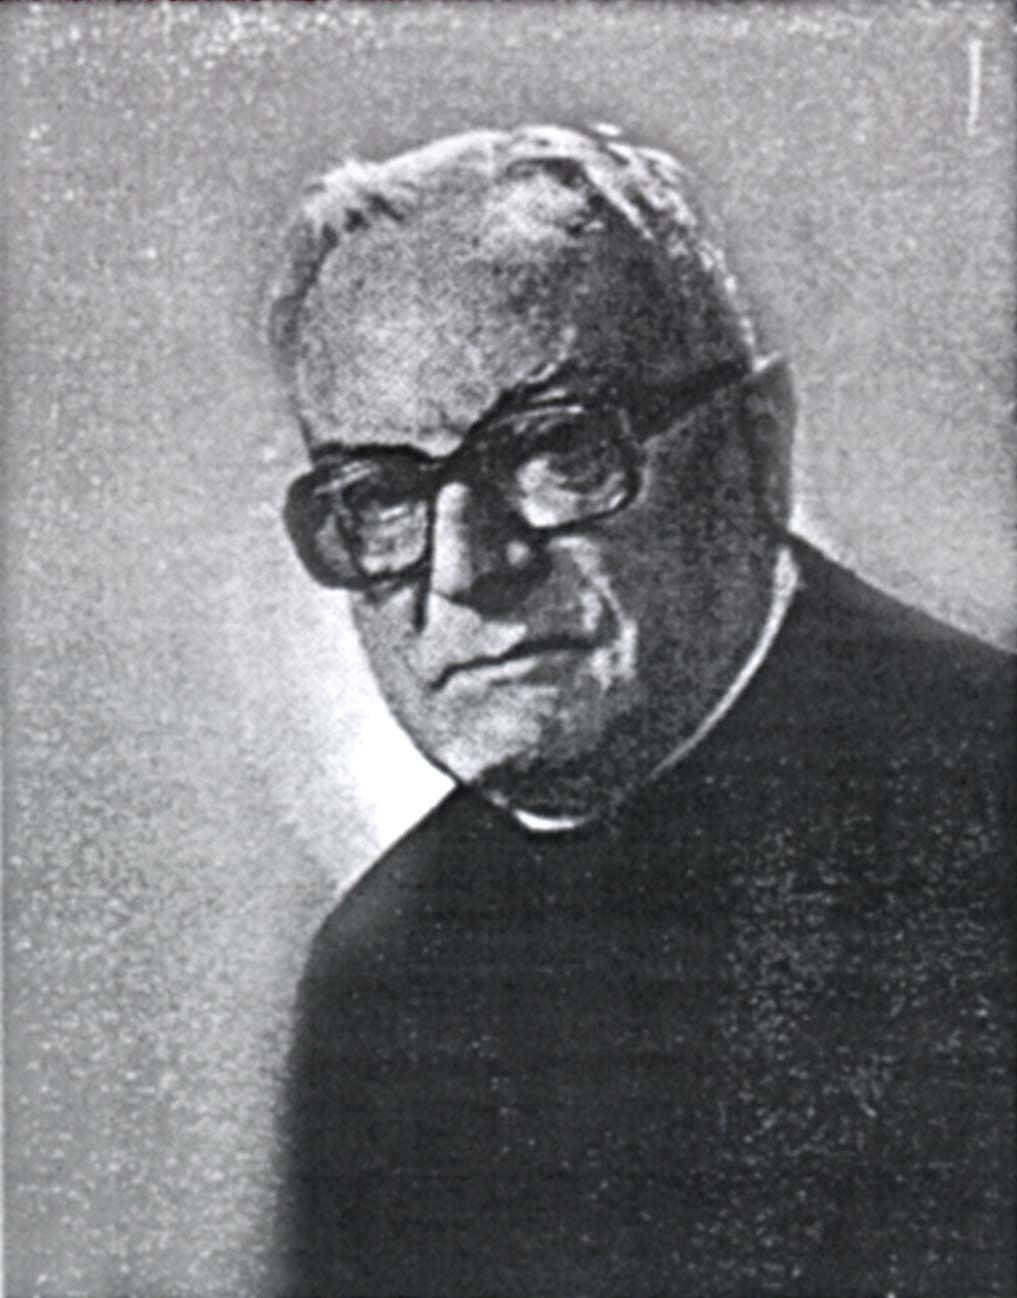
\includegraphics[width=3.605cm,height=4.6cm]{pictures/zulassungsarbeit-img045.jpg}

\end{center}
Ferdinand Haberl\\
\end{supertabular}
\end{flushleft}

\begin{figure}
\img{}
\caption{}
\end{figure}

August Högn war nicht nur auf heimatkundlichem Gebiet schriftstellerisch
tätig. Es gibt Anzeichen dafür, dass er sich auch mit musikhistorischen
Themen beschäftigt haben könnte. Ein Briefwechsel aus dem Jahr 1947 mit
Ferdinand Haberl, Direktor der Kirchenmusikschule in Regensburg, in dem
es um die Entstehung und Herkunft des Weihnachtsliedes „Stille Nacht“
geht, unterstreicht diese Annahme. \footnote{Dokument Nr. 65, Brief von
August Högn an Dr. Haberl, Regensburg, Mrz. 1947; Dokument Nr. 61,
Brief von F. Mitterwallner, Deggendorf an August Högn, 25.2.1947}

\subsection{Unwürdiger Abschied als Chorregent}

\hypertarget{RefHeadingToc100333737}{}Ähnlich große Wellen wie die
Entlassung des Chorregenten Max Rauscher im Jahr 1927 schlug 1953
August Högns Ausscheiden als Kirchenchorleiter. Dem Chorleiterwechsel
ging ein Pfarrerwechsel voraus. Am 17. Februar 1953 verstarb Pfarrer
Jakob Bauer. \footnote{Reicheneder-Chronik, Seelsorger, Blatt III/14
(4) Vorderseite} Der neue Pfarrherr Franz Seraph Reicheneder wurde am
26. Mai 1953 in Ruhmannsfelden empfangen und am 14. Juni\footnote{
Reicheneder-Chronik, Seelsorger, Blatt III/15 (1) Vorderseite}
schließlich feierlich mit Högns „Josephi“-Messe installiert.\footnote{
Dokument Nr. 41, Zeitungsartikel aus dem Viechtacher Bayerwald-Boten,
15.6.1953} August Högn wollte eigentlich bei Antritt des neuen Pfarrers
seinen Rücktritt als Chorregent und Organist bekannt geben, doch der
neue Pfarrer lehnte sein Ersuchen anstandsgemäß ebenso wie vor einiger
Zeit Pfarrer Jakob Bauer und in der Übergangszeit Pfarrprovisor Georg
Huber ab. \footnote{Dokument Nr. 18, Brief von August Högn an Pfarrer
Reicheneder, 25.1.1954} August Högns Rücktrittsabsichten sprachen sich
sogar herum, sodass Josef Brunner – er war während der Kriegszeit
Aushilfsorganist in Ruhmannsfelden – eine Bewerbung für die
möglicherweise frei werdende Chorregentenstelle bei der
Kirchenverwaltung Ruhmannsfelden einreichte. \footnote{Dokument Nr. 17,
Brief von Josef Brunner an Kirchenverwaltung, 29.4.1953}

\begin{center}
\begin{minipage}{4.032cm}
\begin{flushleft}
\tablefirsthead{}
\tablehead{}
\tabletail{}
\tablelasttail{}
\begin{supertabular}{m{3.832cm}}

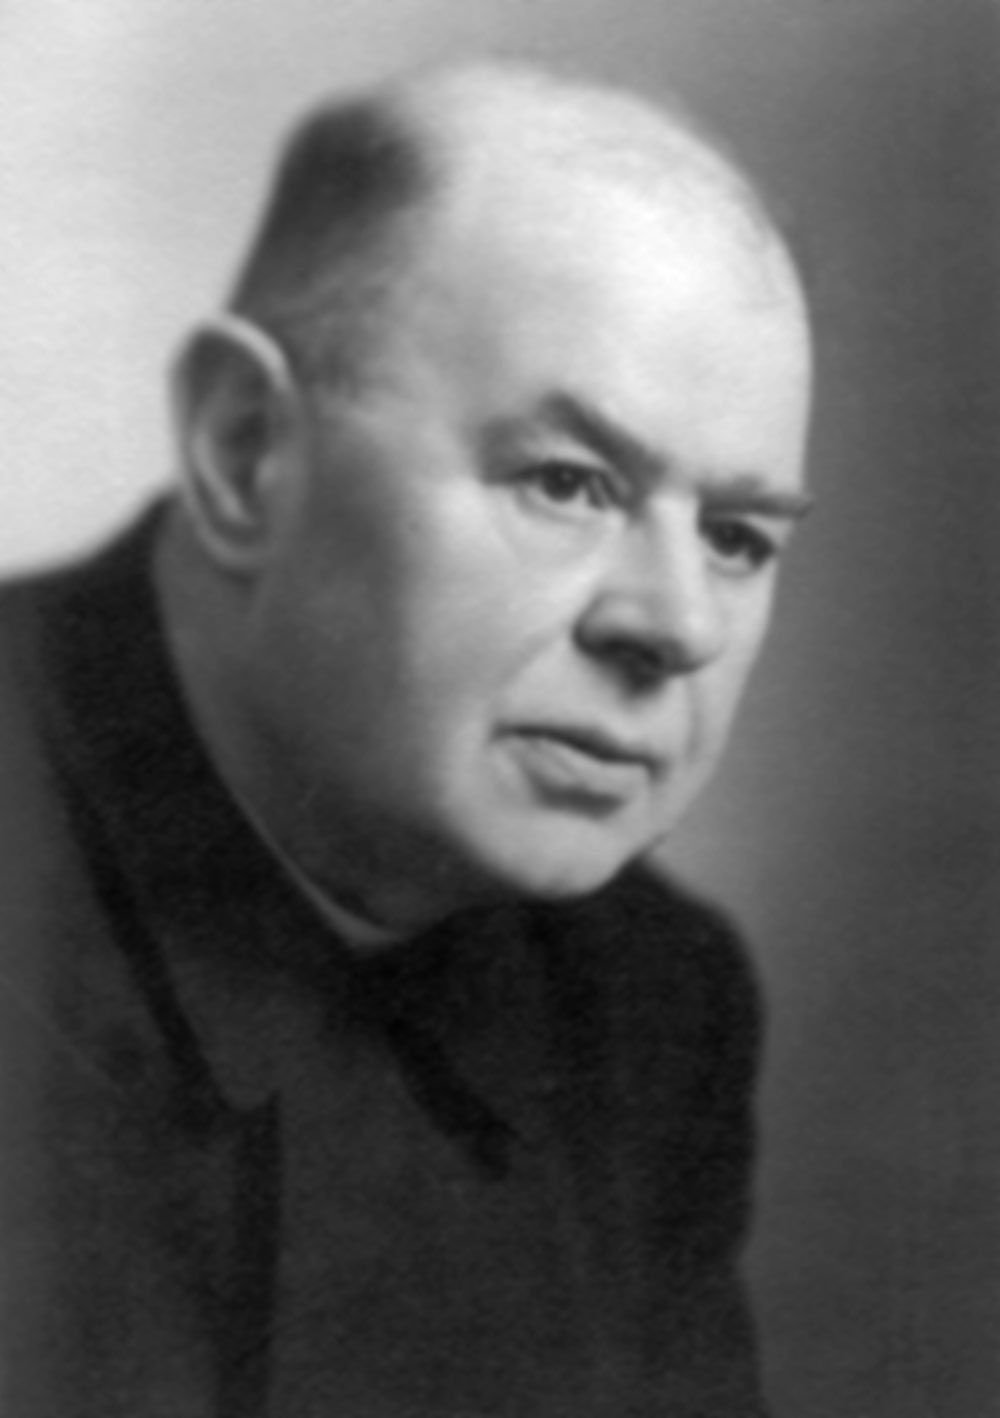
\includegraphics[width=3.651cm,height=5.177cm]{pictures/zulassungsarbeit-img046.jpg}

Abb. \stepcounter{Abb}{\theAbb}: Jakob Bauer\\
\end{supertabular}
\end{flushleft}
\end{minipage}
\end{center}
Umso verwunderlicher ist die Dramatik wie sich Högns Ausscheiden als
Chorregent dann tatsächlich vollzog: Nachdem Högns Bitte um Rücktritt
von Pfarrer Reicheneder abgelehnt wurde, scheint Högn weiterhin mit
einer längerfristigen Dienstzeit als Chorregent und Organist gerechnet
zu haben, sonst hätte er nicht schon 1953 zwei Marienlieder zum
marianischen Jahr 1954 komponiert. Reicheneder hingegen, von Högns
Amtsmüdigkeit überzeugt, war wahrscheinlich davon ausgegangen, dass der
75-jährige Högn bald abdankt würde. \footnote{Interview Nr. 24, Johann
Glasschröder, 28.12.2004, Absatz 48} Vielleicht hatte er auch schon
deswegen seiner von vorneherein favorisierter Nachfolgerin Maria
Reisinger eine baldige Anstellung in Aussicht gestellt. Maria
Reisinger, ein Waisenkind, war Reicheneders Ziehtochter, um deren
Ausbildung sich Reichender gekümmert hatte.

Mit Sicherheit hat Reicheneder die Ablehnung des Rücktrittsgesuchs aus
folgenden zwei Gründen bereut: Zum einem war für seine Ziehtochter
keine Anstellung in absehbarer Zeit greifbar, zum anderen leisteten zum
damaligem Zeitpunkt Högn und sein Chor äußerst schlechte Darbietungen.
Die Aufführung der „Josephi“-Messe durch den
\zitat{„klangvollen Chor“}
\footnote{Dokument Nr. 41, Zeitungsartikel aus dem Viechtacher
Bayerwald-Boten, 15.6.1953} zu Reicheneders Installation war nicht
repräsentativ für den alltäglichen Kirchenmusikbetrieb, da hier viele
Aushilfen mitwirkten \footnote{Interview Nr. 24, Johann Glasschröder,
28.12.2004, Absatz 44} und hatte möglicherweise bei Reicheneder ein
falschen Eindruck hinterlassen.

\begin{flushleft}
\tablefirsthead{}
\tablehead{}
\tabletail{}
\tablelasttail{}
\begin{supertabular}{m{3.5939999cm}m{4.361cm}m{4.123cm}m{3.3769999cm}}

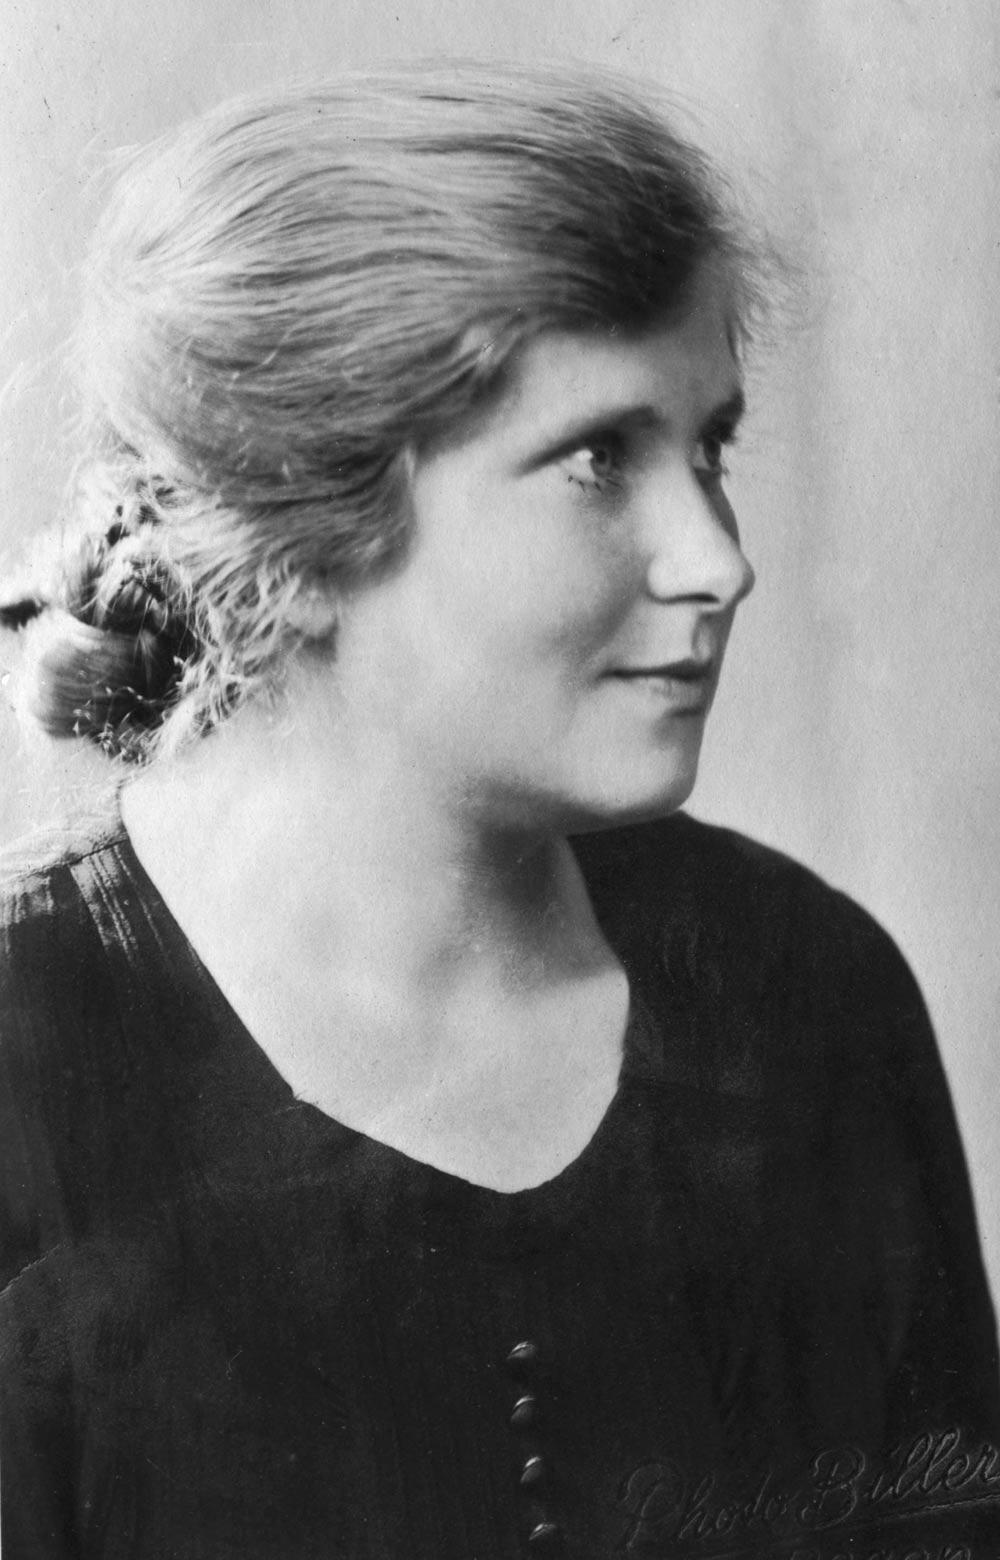
\includegraphics[width=3.413cm,height=5.323cm]{pictures/zulassungsarbeit-img047.jpg}

Abb. \stepcounter{Abb}{\theAbb}: Der „Chor“ der Nachkriegszeit: Mathilde
Glasschröder &

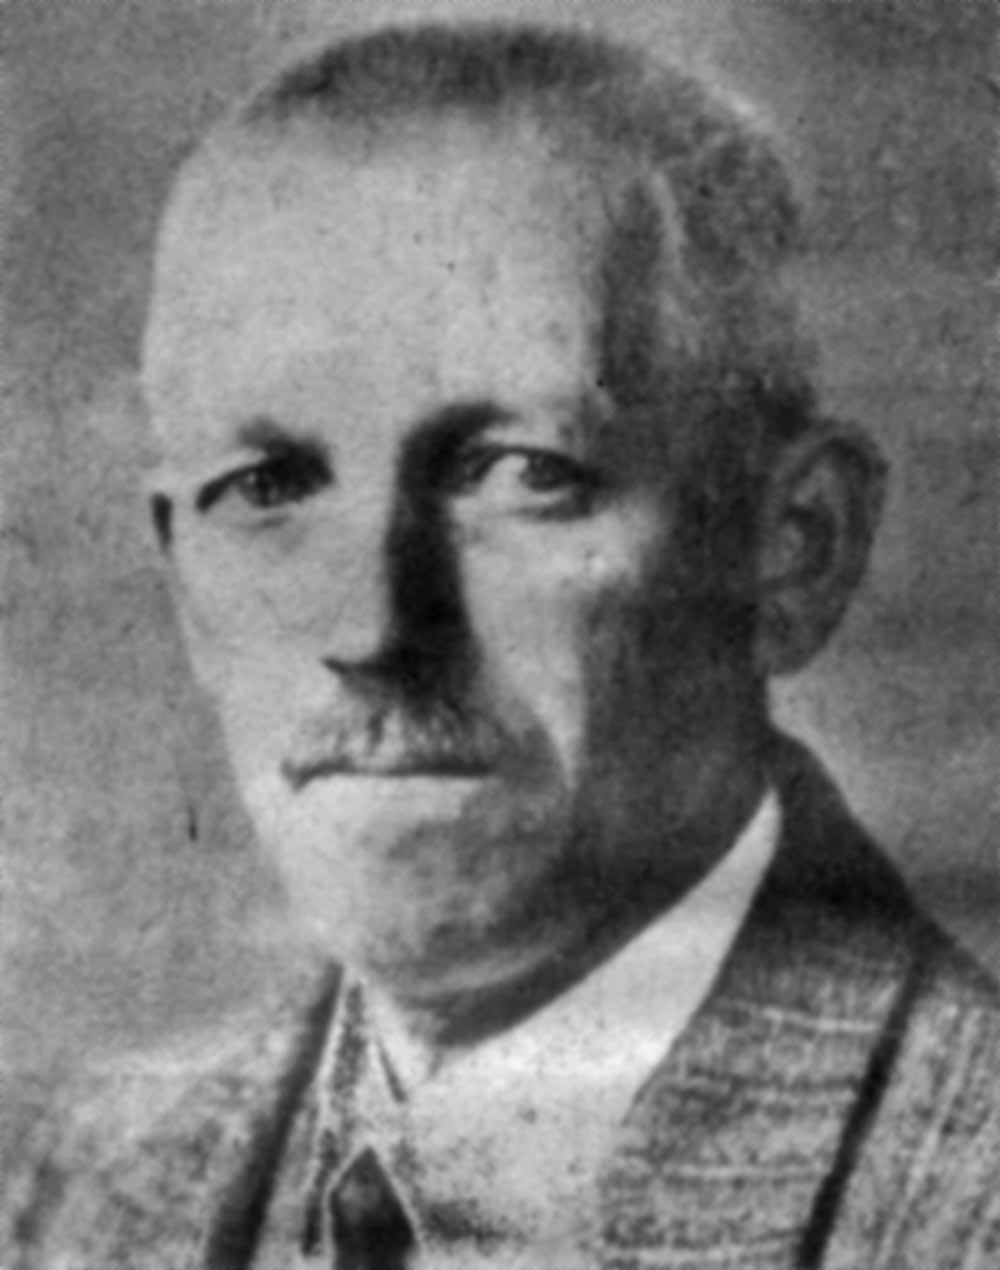
\includegraphics[width=4.18cm,height=5.308cm]{pictures/zulassungsarbeit-img048.jpg}

Abb. \stepcounter{Abb}{\theAbb}: August Högn &

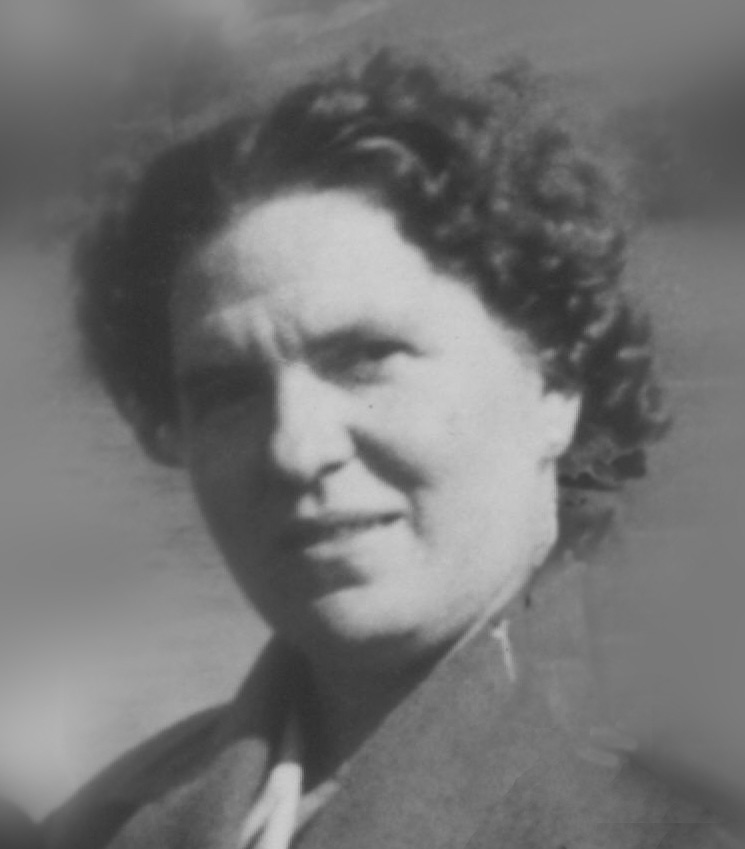
\includegraphics[width=3.942cm,height=5.3cm]{pictures/zulassungsarbeit-img049.jpg}

Abb. \stepcounter{Abb}{\theAbb}: Barbara Essigmann  &

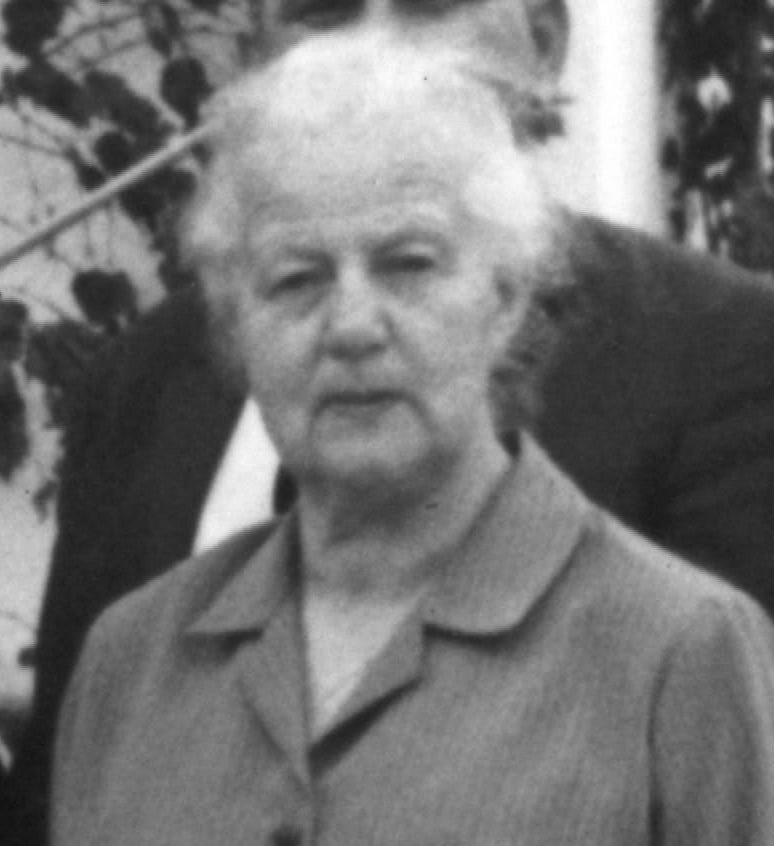
\includegraphics[width=3.194cm,height=5.281cm]{pictures/zulassungsarbeit-img050.jpg}

Abb. \stepcounter{Abb}{\theAbb}: Theres Raster\\
\end{supertabular}
\end{flushleft}
Der „Chor“, der unter der Woche sang, bestand nur aus vier Personen: Den
drei Sängerinnen Mathilde Glasschröder, Barbara Essigmann, Theres
Raster, und August Högn, der selbst eine Männerstimme
übernahm. \footnote{Interview Nr. 24, Johann Glasschröder, 28.12.2004,
Absatz 2} Vor allem die Heterogenität der einzelnen Stimmen
untereinander, die durch die Kleinstbesetzung unverdeckt hervortrat,
hinterließ bei so manchen Kirchenbesuchern einen schlechten
Eindruck. \footnote{Interview Nr. 9, Dr. Doraliesa Wiegmann, 19.1.2003,
Absatz 4; Interview Nr. 24, Johann Glasschröder, 28.12.2004, Absatz 36}
Wurde Mathilde Glasschröder als sängerische Naturbegabung mit großer
Stimme vergleichbar einer Opernsängerin beschrieben,\footnote{
Interview Nr. 13, Lorenz Schlagintweit, 29.11.2003, Absatz 2; Interview
Nr. 24, Johann Glasschröder, 28.12.2004, Absatz 52} blieb Theres Raster
als außerordentlich schlechte Sängerin mit „fürchterlichem“ Stimmklang
in Erinnerung. \footnote{Interview Nr. 24, Johann Glasschröder,
28.12.2004, Absatz 46} Die alternde Stimme Högns scheint sich ebenso
wenig in einen Gesamtklang eingebunden zu haben. \footnote{Interview
Nr. 24, Johann Glasschröder, 28.12.2004, Absatz 36} Neben dem
schlechtem Gesang stellte für Reicheneder möglicherweise das
kirchenmusikalische Repertoire einen Stein des Anstoßens dar. Ein und
dasselbe Lied, das zum Schluss des Gottesdienstes gesungen wurde, hatte
sich als „Standardstück“ eingebürgert \footnote{Interview Nr. 16, Maria
Freisinger, 25.8.2004, Absatz 20} und nicht nur werktags wurden Teile
aus dem Gloria und Credo übersprungen. \footnote{Interview Nr. 24,
Johann Glasschröder, 28.12.2004, Absatz 26; Interview Nr. 2, Barbara
Essigmann, 27.12.2002, Absatz 36; Interview Nr. 16, Maria Freisinger,
25.8.2004, Absatz 14}

Obwohl in Ruhmannsfelden die Bereitschaft zum Singen recht groß war – es
gab neben dem Kirchenchor einen Männerchor und eine weltliche
Liedertafel \footnote{Interview Nr. 24, Johann Glasschröder,
28.12.2004, Absatz 10, 4 } – gab es in Ruhmannsfelden lediglich ein
Gesangsquartett als Kirchenchor. Reicheneder muss als Hauptgrund für
diesen Missstand die laxe Probenpraxis in Högns Wohnung angesehen
haben, den er durch Ansetzung von öffentlichen Proben zu beseitigen
versuchte – wohl bemerkt mit Högn als Chorleiter. \footnote{Interview
Nr. 24, Johann Glasschröder, 28.12.2004, Absatz 43 – 44} Es ist höchst
ungewöhnlich, wenn nicht ein Chorleiter selbst über die Anberaumung der
Chorproben entscheidet. Einerseits wollte Reicheneder durch diese
Maßnahme wahrscheinlich, das Niveau der musikalischen Darbietungen
erhöhen. Andererseits hoffte er doch insgeheim, dass Högn durch diese
Bevormundung abdankt und die Stelle für seine Vertrauensperson Maria
Reisinger frei macht. Die mit Högn sehr eng befreundeten
Chorsängerinnen Mathilde Glasschröder und Barbara Essigmann erschienen
nicht zu den von Reicheneder festgesetzten Proben \footnote{Interview
Nr. 24, Johann Glasschröder, 28.12.2004, Absatz 42} und lieferten somit
Reicheneder einen Grund zum Einschreiten.

In seinen Briefen an beide Chorsängerinnen und in diesem Fall auch an
Högn teilte Reicheneder allen drei kurz vor Weihnachten 1953 ihre
„Kündigung“ mit. Soweit der Inhalt der Briefe aus Augenzeugenberichten
erahnt werden kann, war zwar in ihnen kein Wort von „Kündigung“ zu
lesen, da aber Reicheneder den Sängerinnen und Högn die Chorabrechnung
beifügte und ihnen für ihre Dienste an der Pfarrkirche Ruhmannsfelden
dankte, machte er ihnen unmissverständlich deutlich, dass er für sie
keinen weiteren Einsatz in der Kirchenmusik vorsah. \footnote{Interview
Nr. 24, Johann Glasschröder, 28.12.2004, Absatz 38 – 40} Diese
„Kündigungsschreiben“ verursachten bei den Betroffenen große
Verärgerung. Als Högn seinen Brief den zwei Sängerinnen zeigte, soll er
Reicheneder sogar als \zitat{„Lackel“} bezeichnete
haben. \footnote{Interview Nr. 2, Barbara Essigmann, 27.12.2002, Absatz
64} Die Verärgerung der Sängerinnen schlug in Hass auf Reicheneder
um, \footnote{Interview Nr. 2, Barbara Essigmann, 27.12.2002, Absatz
16} nachdem wenig später „ihr Högn“ einen schweren Schlaganfall erlitt,
der eine linksseitige Lähmung zur Folge hatte, \footnote{Dokument Nr.
73, Brief von August Högn an Stephan Leitner, 10.3.1961} und in ein
Krankenhaus gebracht werden musste. \footnote{Interview Nr. 24, Johann
Glasschröder, 28.12.2004, Absatz 36} Beide Sängerinnen gaben
Reicheneder die Mitschuld an Högns Schlaganfall. Ein Foto von 1961
zeigt auch deutlich, dass Högn an einer leichten Gesichtslähmung als
Spätfolge des Schlaganfalls litt, und Zeitzeugen berichten von
Beeinträchtigungen beim Sprechen. \footnote{Interview Nr. 2, Barbara
Essigmann, 27.12.2002, Absatz 36} Nur mit Zuhilfenahme eines
Stocks \footnote{Foto bei der Einweihung des Schulanbaus, 7.5.1959}
konnte Högn seitdem gehen. \footnote{Interview Nr. 2, Barbara
Essigmann, 27.12.2002, Absatz 38, 62, 64} An Orgelspielen war nicht
mehr zu denken.

\begin{center}
\begin{minipage}{10.084cm}
\begin{flushleft}
\tablefirsthead{}
\tablehead{}
\tabletail{}
\tablelasttail{}
\begin{supertabular}{m{5.018cm}m{4.6670003cm}}

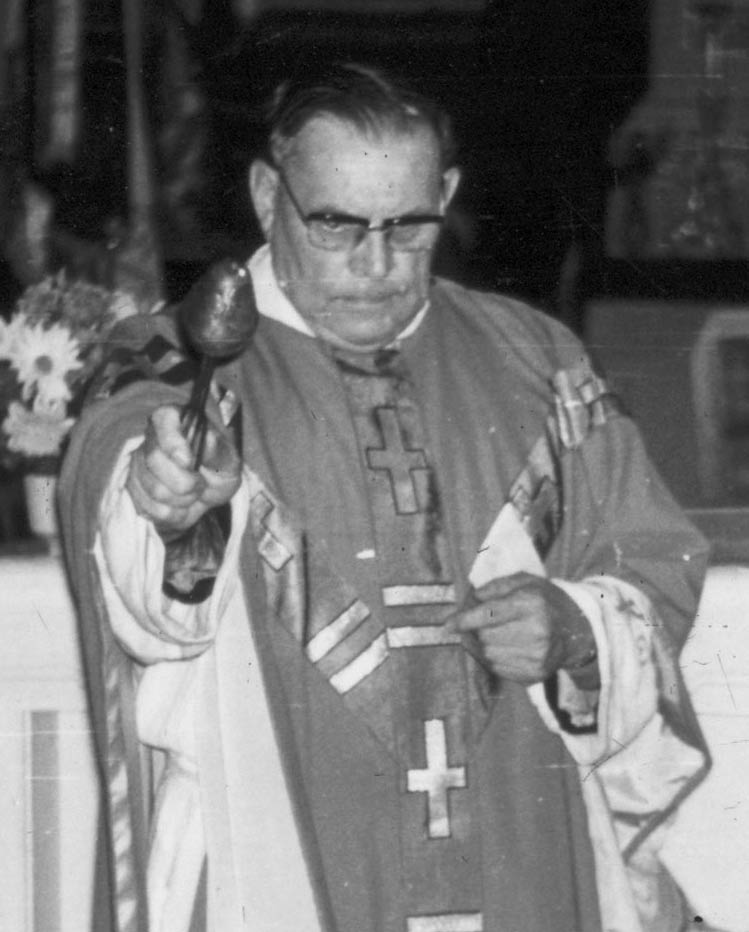
\includegraphics[width=4.835cm,height=5.992cm]{pictures/zulassungsarbeit-img051.jpg}

Abb. \stepcounter{Abb}{\theAbb}: Franz Seraph Reicheneder &

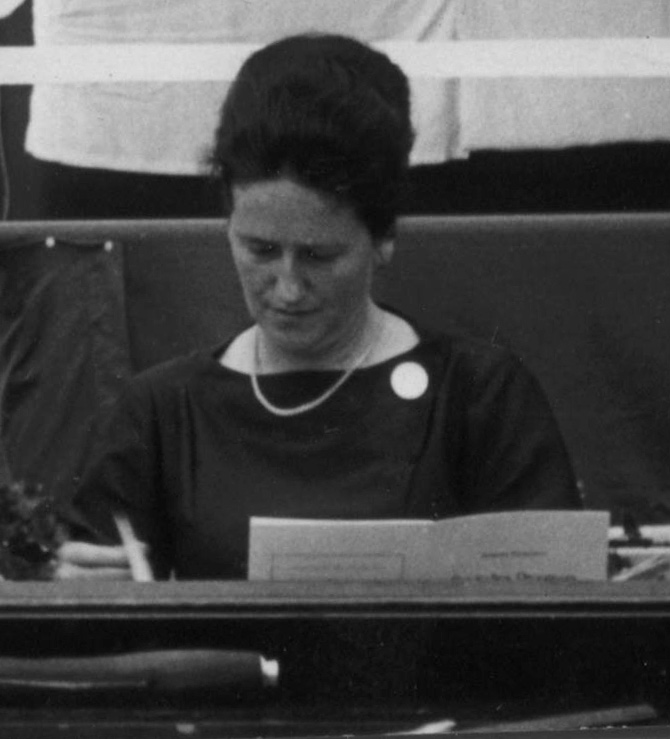
\includegraphics[width=4.484cm,height=6.003cm]{pictures/zulassungsarbeit-img052.jpg}

Abb. \stepcounter{Abb}{\theAbb}: Maria Reisinger\\
\end{supertabular}
\end{flushleft}
\end{minipage}
\end{center}
Deshalb wirkt der Brief, den Högn nach seinem Krankenhausaufenthalt am
25.1.1954 an Reicheneder schrieb, schon etwas befremdlich. Mit der
\zitat{„berechtigten Forderung auf Ruhestand auch im
Kirchenchordienst“} verkündete Högn in diesem Schreiben seinen
Rücktritt als Chorregent und Organist und bezog sich dabei nicht auf
die Folgen seines Schlaganfalls oder auf das „Kündigungsschreiben.“
 \footnote{Dokument Nr. 18, Brief von August Högn an Pfarrer
Reicheneder, 25.1.1954} In seinem Antwort-Brief vom 6.2.1954 nahm
Reicheneder zu Högns erhaltenen Brief Stellung, in dem Högn von sich
aus abdankte, und unterstrich, dass er Högns
\zitat{„Standpunkt voll und ganz verstehen“} könne, seinen
Rücktritt aber \zitat{„sehr bedauere.“ } \footnote{Dokument
Nr. 19, Brief von Pfarrer Reicheneder an August Högn, 6.2.1954}

Wären nur diese zwei Briefe und nicht zusätzlich die genauen
Erinnerungen von mehreren Zeitzeugen zur Verfügung gestanden, hätte man
eine ganz andere Schlussfolgerung daraus gezogen. Sowohl Reicheneder
als auch Högn waren daran interessiert, der Nachwelt eine andere
Version des Ausscheidens Högns als die der Kündigung durch Reicheneder
zu überlassen. Nur zwischen den Zeilen, kann man in beiden Briefen die
vorhergehenden Ereignisse erahnen, wie zum Beispiel an der Stelle, an
der Högn die \zitat{„Kündigung seitens des Hochwürdigen Herr
Pfarrers und der gleichen“} als \zitat{„blödes
Weibergeschwätz“} bewertet und darauf hinweist, dass
\zitat{„eine vertragliche Abmachung über den
Kirchenchordienst zwischen Pfarramt Ruhmannsfelden“ }und ihm niemals
bestanden hätte.“  \footnote{Dokument Nr. 18, Brief von August Högn an
Pfarrer Reicheneder, 25.1.1954}\zitat{ }Und seine angebliche
\zitat{„Stimmbandlähmung“,} \footnote{Dokument Nr. 19, Brief
von Pfarrer Reicheneder an August Högn, 6.2.1954}\zitat{ }die
Reicheneder als Entschuldigung anführte, weshalb er Högn keinen
Krankenbesuch abstattete, erscheint in diesem Zusammenhang mehr als
eine faule Ausrede.

Über den wahren Wortlaut der „Kündigungsbriefe“ ließe sich natürlich
viel spekulieren. Allein schon ihr Verschwinden ist ein Beweis für ihre
Brisanz. Reicheneder war ein passionierter Historiker und Archivar. Es
gibt wohl keinen auf die hiesige Gegend bezogenen Zeitungsartikel aus
Reicheneders Ruhmannsfeldener Zeit, der nicht in seine über 30 prall
gefüllte Ordner umfassende „Chronik Ruhmannsfelden“ angefügt wurde.
Auch seine Korrespondenz dokumentierte Reicheneder sehr genau. Viele
von ihm verfasste Briefe lassen sich im Pfarrarchiv im
Kohlepapierabdruck nachlesen, wie etwa das Schreiben an Högn vom
6.2.1954. Die „Kündigungsschreiben“ hat Reicheneder ganz bewusst nicht
archiviert, damit kein schlechtes Licht auf ihn fällt. Einen kaum
unwürdigeren Abschied hätte Reicheneder Högn nach 43 Jahren Dienstzeit
an der Kirchenmusik in Ruhmannsfelden nicht bieten können.

Diese ungerechte Vorgehensweise von Reicheneder gegenüber Högn ist kein
Einzelfall. Ein Ereignis wenige Jahre später ist bezeichnend für
Reicheneders Problemlösungsstrategie mit der „Brechstange“: Nachdem
Pfarrer Reicheneder bei einer Sonntags-Predigt von der Kanzel aus unter
anderem über die \zitat{„Leistungsabzeichen für nächtliche
Liebesfahrten“} \footnote{
http://home.vrweb.de/pfarrei.ruhmannsfelden/reichene.htm} wetterte, die
am Fußballer Ball 1957 verliehen wurden, ließen sich die Beschuldigten
nicht zurechtweisen und veranstalten, nach Angaben des Geistlichen
selbst, aus einer Trotzreaktion heraus ein Faschingsbegräbnis am
Aschermittwoch mit Musik und Saufgelage. \zitat{„Bis die
Haupträdelsführer beim Pfarramt vorstellig geworden sind“;}\footnote{
http://home.vrweb.de/pfarrei.ruhmannsfelden/reichene.htm} wie es in
einer Pressemitteilung des Pfarramts hieß, sollten nun die Glocken in
Ruhmannsfelden schweigen. Diese Aktion machte natürlich nicht nur in
der regionalen Presse ihre Runde. Die Glocken läuteten erst wieder, als
sich der Bürgermeister von Ruhmannsfelden in den Fall einbezog und für
eine Lösung des Problemfalls sorgte, die schriftlich festgehalten
wurde.\footnote{
http://home.vrweb.de/pfarrei.ruhmannsfelden/reichene.htm}

In der Kirchenverwaltungssitzung vom 21.2.1954 wurde Högns Nachfolge
endgültig geregelt. Maria Reisinger erhielt die Organistenstelle und
Franz Danziger übernahm die Chorleitung. \footnote{Dokument Nr. 124,
Protokoll der Kirchenverwaltungssitzung, 21.2.1954}

\subsection{Die letzten Lebensjahre}

\hypertarget{RefHeadingToc100333738}{}  [Warning: Image ignored]
% Unhandled or unsupported graphics:
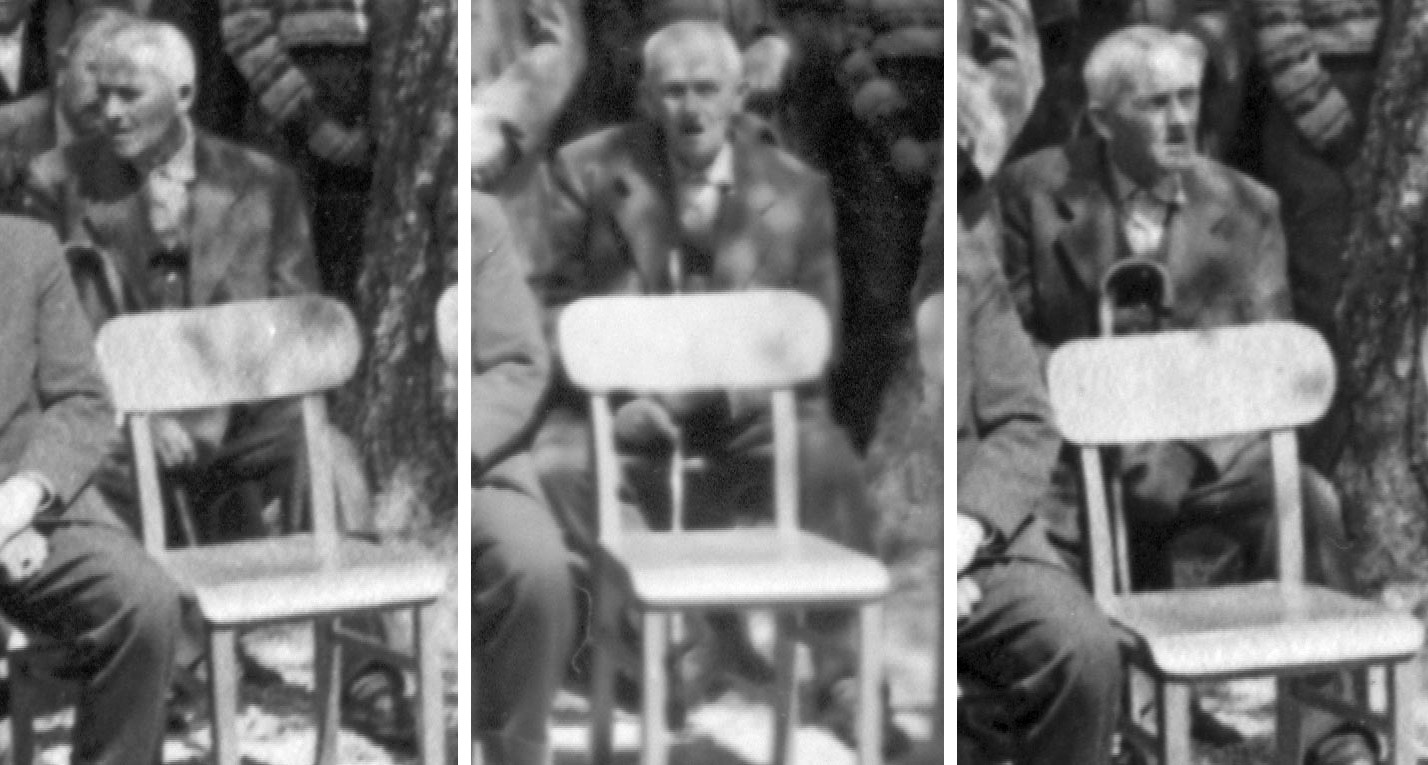
\includegraphics[width=15.981cm,height=8.56cm]{pictures/zulassungsarbeit-img053.jpg}


Abb. \stepcounter{Abb}{\theAbb}: August Högn auf Bildern, die zur
Einweihung des Schulanbaus an Christihimmelfahrt 1959 aufgenommen
wurden.

Einen tiefen Einschnitt in Högns unruhiges Rentnerleben stellte sein
Schlaganfall Ende 1953 dar. Sein Ruhestand, der eigentlich schon 1945
mit der Suspendierung vom Schuldienst infolge der Entnazifizierung
begann und nur durch einen kurzen Schuleinsatz 1947 \footnote{Dokument
Nr. 48, Zeitungsartikel aus Viechtacher Bayerwald-Bote, 2.8.1958}
unterbrochen wurde, konnte vor 1953 wohl kaum als solcher bezeichnet
werden, wenn man seine Aktivitäten für die Kirche und Heimatkunde
betrachtet.

Vieles spricht dafür, dass Högn trotz seiner körperlichen
Beeinträchtigungen ab 1954 ein aktives Leben führte. Er war sogar noch
schöpferisch tätig, wie sein Marienlied „Ruf an die Christenheit“
beweist, das zur 300. Jahrfeier des Osterbrünnls 1960 entstanden ist.
Einige weltliche Kompositionen, die nicht erhalten sind, hat Högn nach
seinem 80. Geburtstag für den Ruhmannsfeldener Männerchor
geschrieben. \footnote{Dokument Nr. 49, Zeitungsartikel aus Viechtacher
Bayerwald-Bote, 5.8.1958; Interview Nr. 24, Johann Glasschröder,
28.12.2004, Absatz 32} Auf eine rege Korrespondenz lassen die vier
langen Briefe schließen, die Högn einem ehemaligen Schüler bis nach
Australien schickte. Sein großes Interesse am öffentlichen Leben in
Ruhmannsfelden belegen die vielen Details aus dem Ortsgeschehen, die
Högn in die Briefe mit einfließen ließ. Kurz vor seinem Tod kaufte er
sich einen Fernsehapparat und konnte sich so über die Außenwelt
informieren. \footnote{Dokument Nr. 73, Brief von August Högn an
Stephan Leitner, 10.3.1961}

In seinen letzten Briefen kommt ein gewisser Schwermut deutlich zum
Ausdruck. Selbst Feste wie Weihnachten findet er
\zitat{„langweilig und ohne Abwechslung“ } \footnote{Dokument
Nr. 70, Brief von August Högn an Stephan Leitner, 9.1.1960} und beklagt
sich, dass der Fasching in Ruhmannsfelden \zitat{„ziemlich
mau“} \footnote{Dokument Nr. 71, Brief von
August Högn an Stephan Leitner, 15.3.1960}\zitat{ }war.
Sehnsucht nach seiner an der Donau gelegenen Heimatstadt Deggendorf
macht sich breit, wenn er schreibt: \zitat{„An den Bergen des
bayerischen Waldes habe ich schon genug. Möchte lieber hinaus in die
Ebene, an die Donau, zum Wasser.“}\footnote{
Dokument Nr. 72, Brief von August Högn an Stephan Leitner, Dez. 1960}
Seine Gedanken scheinen oft um den Tod zu kreisen, wenn er als
Neuigkeit schon zu Beginn eines Briefes mehre Todesfälle aufzählt und
resümiert: \zitat{„Bei uns hier ist die Sterblichkeit
ziemlich groß.“ } \footnote{Dokument Nr. 72, Brief von August Högn an
Stephan Leitner, Dez. 1960}

\begin{center}
\begin{minipage}{9.146cm}
\begin{center}
\tablefirsthead{}
\tablehead{}
\tabletail{}
\tablelasttail{}
\begin{supertabular}{m{4.309cm}m{4.4370003cm}}

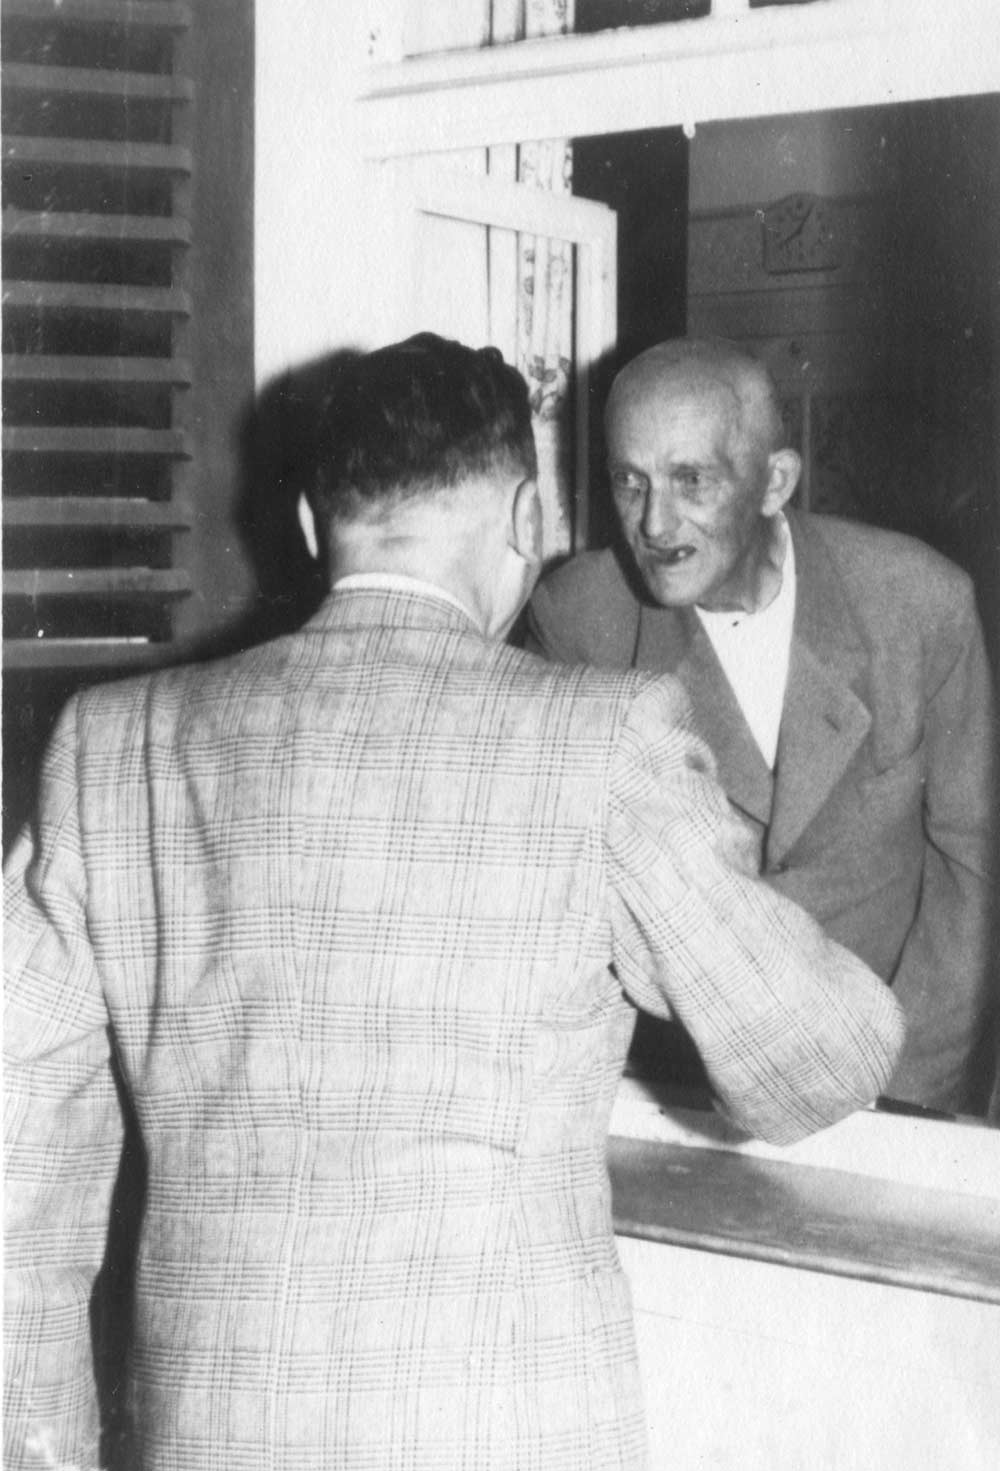
\includegraphics[width=4.128cm,height=6.071cm]{pictures/zulassungsarbeit-img054.jpg}

Abb. \stepcounter{Abb}{\theAbb}: Franz Danziger gratuliert August Högn
am Vorabend zu seinem 80. Geburtstag &

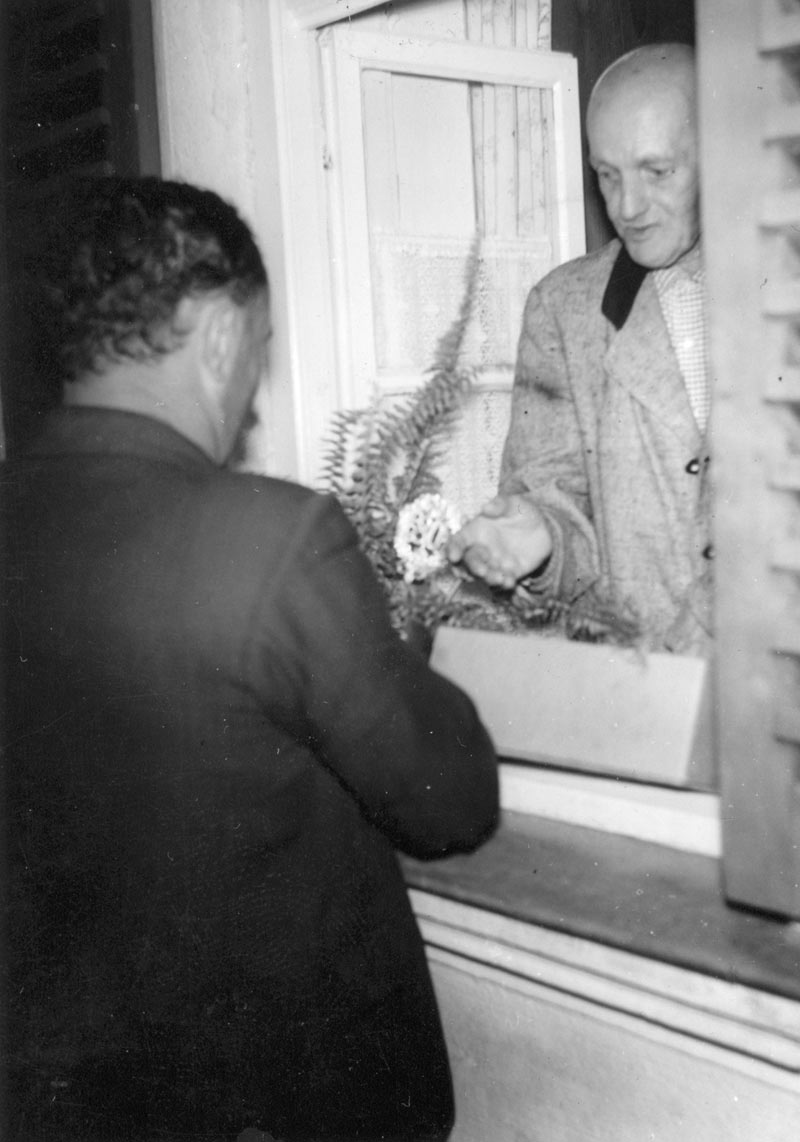
\includegraphics[width=4.255cm,height=6.073cm]{pictures/zulassungsarbeit-img055.jpg}

Abb. \stepcounter{Abb}{\theAbb}: Der Zachenberger Bürgermeister
Bielmeier überreicht August Högn einen Geschenkkorb zum 80.
Geburtstag\\
\end{supertabular}
\end{center}
\end{minipage}
\end{center}
Ende 1960 scheint sich Högns Gesundheitszustand zu verschlechtern. Er
beklagt sich, dass das sein \zitat{„gesundheitliches Befinden
nicht das beste“} ist und das \zitat{„Marschieren sehr
schlecht geht.“ }Um Besserung zu erfahren, sucht er sogar einen Arzt im
mehr als 50 km entfernten Straubing auf. \footnote{Dokument Nr. 72,
Brief von August Högn an Stephan Leitner, Dez. 1960} Er ist immer mehr
auf Hilfe anderer angewiesen und seine Haushälterin Rosa Beischmied
wird zur \zitat{„Krankenfürsorgerin.“ } \footnote{Dokument
Nr. 73, Brief von August Högn an Stephan Leitner,
10.3.1961}Ein letztes Foto von Högn vom Juli
1961 zeigt zwar einen hageren, alten Mann, der an den Folgen seines
Schlaganfalles sichtbar leidet, doch es zeigt keinen vom Tode
gekennzeichneten Mann, der wenige Monate später sterben wird.

August Högn starb am 13. Dezember 1961 um 5 Uhr morgens.\footnote{
Dokument Nr. 50, Zeitungsartikel aus dem Viechtacher Bayerwald-Bote,
14.12.1961} Sein Tod kam nicht plötzlich, da er rechtzeitig mit den
Sterbesakramenten versehen worden war. \footnote{Dokument Nr. 50,
Zeitungsartikel aus dem Viechtacher Bayerwald-Bote, 14.12.1961} Nach
Aussagen von Högns Enkelin Gertraud von Molo war er bis kurz vor seinem
Tod rüstig \footnote{Interview Nr. 20, Gertraud von Molo, 23.11.2004,
Absatz 14} und sein Tod dürfte auf eine eher \zitat{„kürzere
Krankheit“ } \footnote{Interview Nr. 2, Barbara Essigmann, 27.12.2002,
Absatz 62} zurückzuführen sein, als auf eine \zitat{„lange
schwere“}  \footnote{Dokument Nr. 51, Zeitungsartikel aus Viechtacher
Bayerwald-Bote, 15.12.1961} Krankheit, wie es im seinem Nachruf im
Viechtacher Bayerwald-Boten steht. Im Sterberegister der Pfarrei
Ruhmannsfelden steht als Todesursache „Herzinsuffizienz“, was eher auf
einen plötzlichen Tod schließen lässt. \footnote{Dokument Nr. 112,
Eintrag im Sterberegister des Pfarramts Ruhmannsfelden, 13.12.1961}
Waren bei der Überführung des Leichnams am Todestag anwesend\footnote{
Dokument Nr. 51, Zeitungsartikel aus Viechtacher Bayerwald-Bote,
15.12.1961} nur wenige enge Freunde, die dem Leichenauto Richtung
Deggendorf einige hundert Meter folgten, \footnote{Interview Nr. 2,
Barbara Essigmann, 27.12.2002, Absatz 64} so dürfte es beim im
Ruhmannsfelden abgehaltenen Requiem am darauffolgenden Tag in
Ruhmannsfelden ein Großteil der Ruhmannsfeldener Bevölkerung gewesen
sein, der von Högn Abschied nahm. Die Ruhmannsfeldener Volksschule nahm
an der Trauerfeier teil und jeder ehemalige Schüler erhielt eine
Einladung zum Besuch des Trauergottesdienstes. \footnote{Dokument Nr.
50, Zeitungsartikel aus dem Viechtacher Bayerwald-Bote, 14.12.1961} Die
offizielle Beerdigung fand am 15. Dezember in der Deggendorfer
Pfarrkirche Mariä Himmelfahrt statt. \footnote{Dokument Nr. 66,
Todesbenachrichtigung, 13.12.1961} Bei eisiger Kälte\footnote{
Interview Nr. 3, Ida Högn, 29.12.2002, Absatz 20} hielten die Lehrer
Karl Schambeck, \footnote{Dokument Nr. 52, Brief von Elfriede
Schlumprecht an Lehrer Schambeck, 3.1.1962} Franz Nemetz\footnote{
Interview Nr. 3, Ida Högn, 29.12.2002, Absatz 20; Dokument Nr. 53,
Brief von Elfriede Schlumprecht an Rektor Langesee, 3.1.1962} und der
Kreisschulrat Botschafter \footnote{Dokument Nr. 53, Brief von Elfriede
Schlumprecht an Rektor Langesee, 3.1.1962} am Grab Trauerreden auf
August Högn. Besonders die Ansprache von Lehrer Nemetz blieb als eine
sehr lange Rede bei vielen Anwesenden in Erinnerung.\footnote{
Interview Nr. 3, Ida Högn, 29.12.2002, Absatz 20} Abordnungen der
Vereine aus Ruhmannsfelden waren mit Fahnen anwesend und eine
Bläsergruppe der freiwilligen Feuerwehr von Ruhmannsfelden spielte für
ihr Ehrenmitglied zum Abschied das Lied „Wir hatten einen Kameraden.“
 \footnote{Interview Nr. 20, Gertraud von Molo, 23.11.2004, Absatz 42}
August Högn fand seine letzte Ruhestätte auf dem Deggendorf Friedhof,
im schönen Grabmal \footnote{Interview Nr. 20, Gertraud von Molo,
23.11.2004, Absatz 10} neben seiner 1926 verstorbenen Ehefrau Emma.

\begin{center}
\begin{minipage}{5.542cm}
\begin{flushleft}
\tablefirsthead{}
\tablehead{}
\tabletail{}
\tablelasttail{}
\begin{supertabular}{m{5.342cm}}

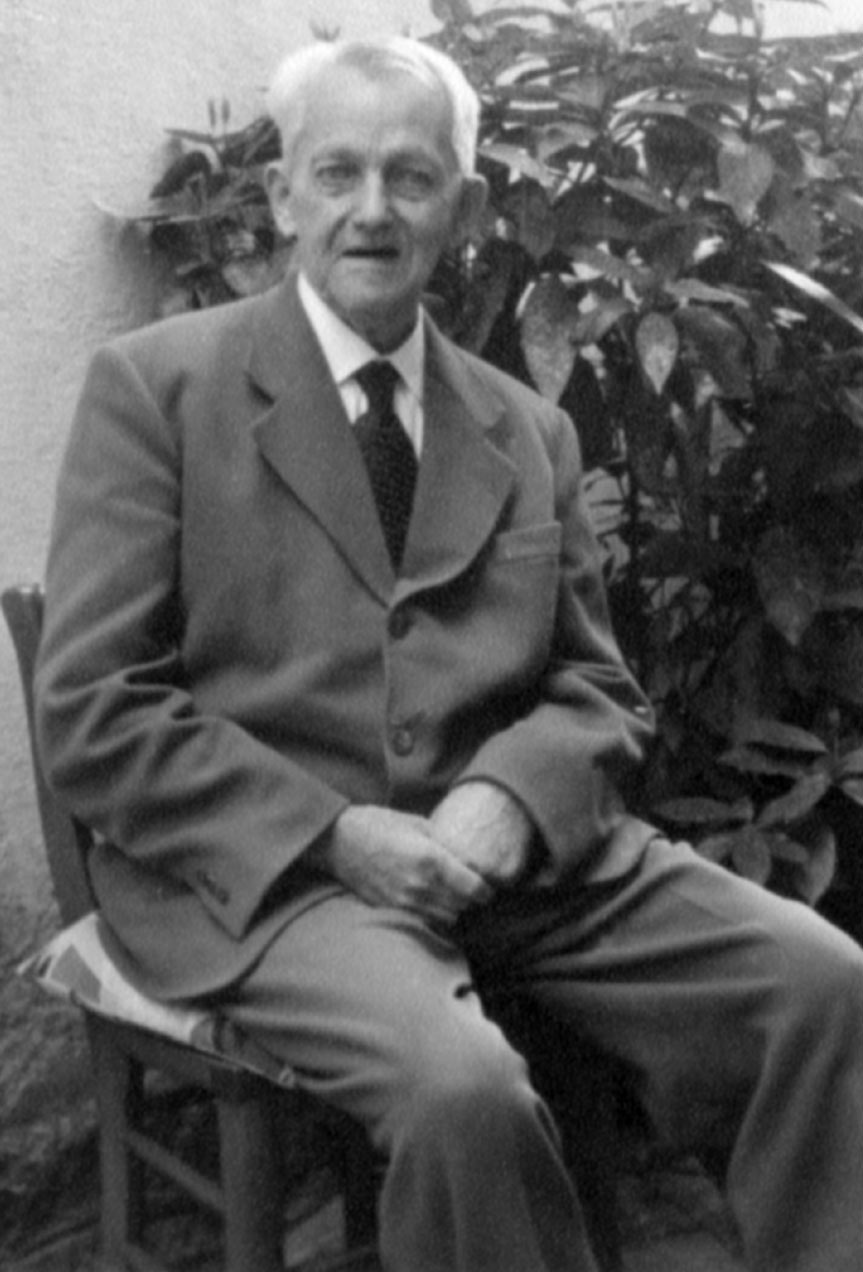
\includegraphics[width=5.159cm,height=7.606cm]{pictures/zulassungsarbeit-img056.jpg}

Abb. \stepcounter{Abb}{\theAbb}: letztes Foto von August Högn, Juli
1961\\
\end{supertabular}
\end{flushleft}
\end{minipage}
\end{center}
\begin{flushleft}
\tablefirsthead{}
\tablehead{}
\tabletail{}
\tablelasttail{}
\begin{supertabular}{m{12.311cm}m{3.6929998cm}}

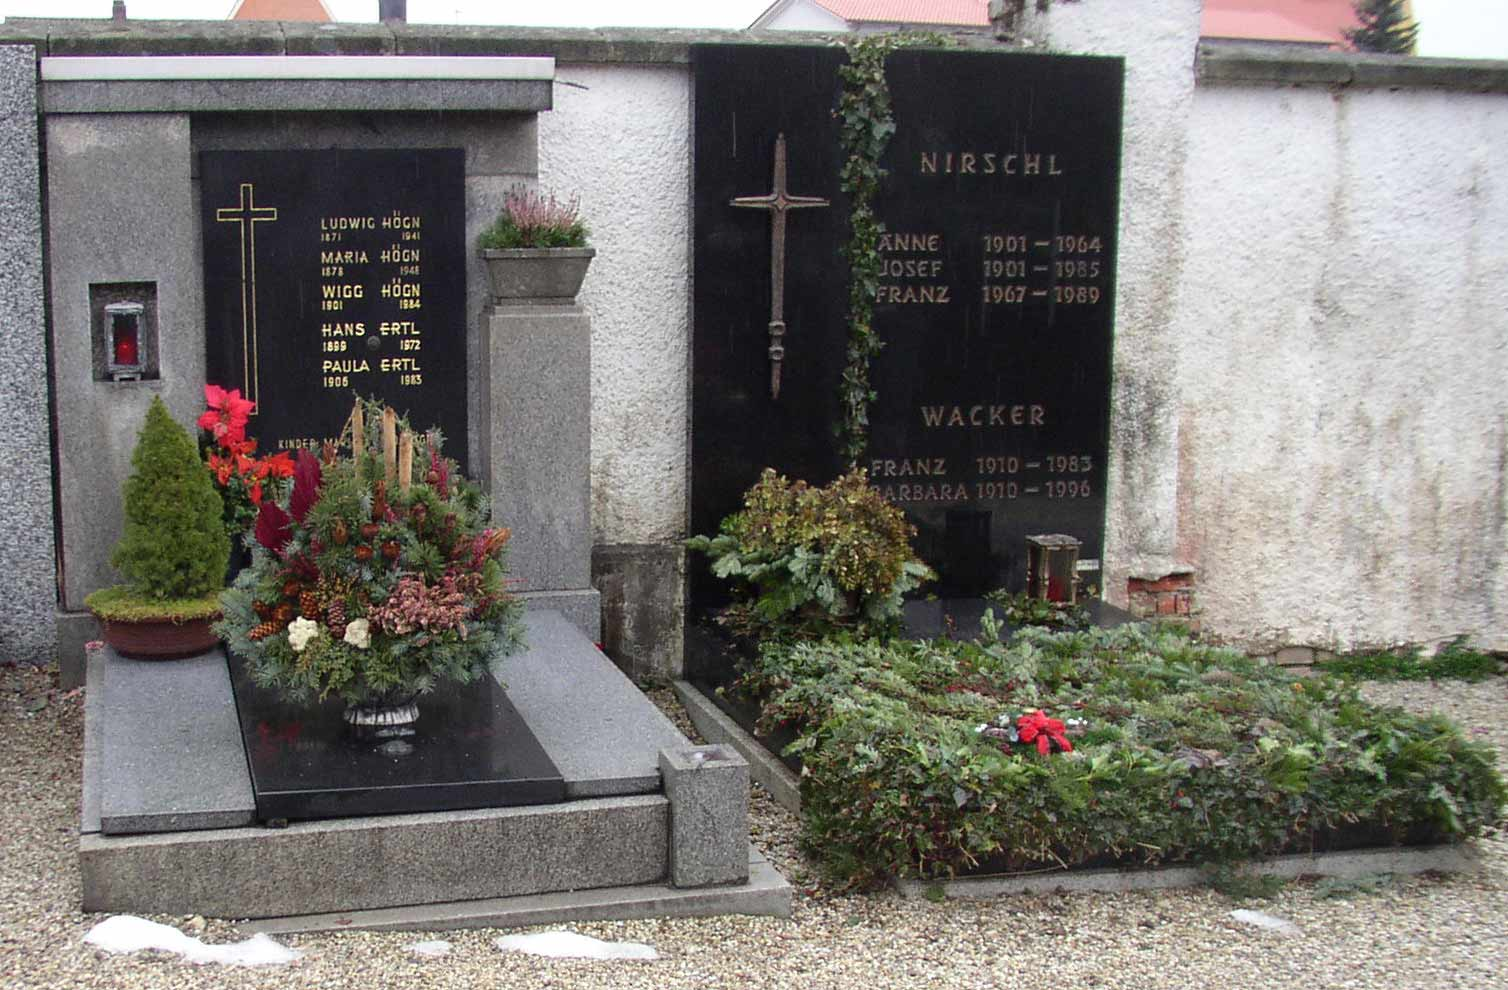
\includegraphics[width=12.129cm,height=8.015cm]{pictures/zulassungsarbeit-img057.jpg}

Abb. \stepcounter{Abb}{\theAbb}: Familiengrab von Ludwig Högn (links)
und ehemalige Grabstätte von August Högn und seiner Ehefrau (rechts),
heute im Besitz der Familie Nirschl &

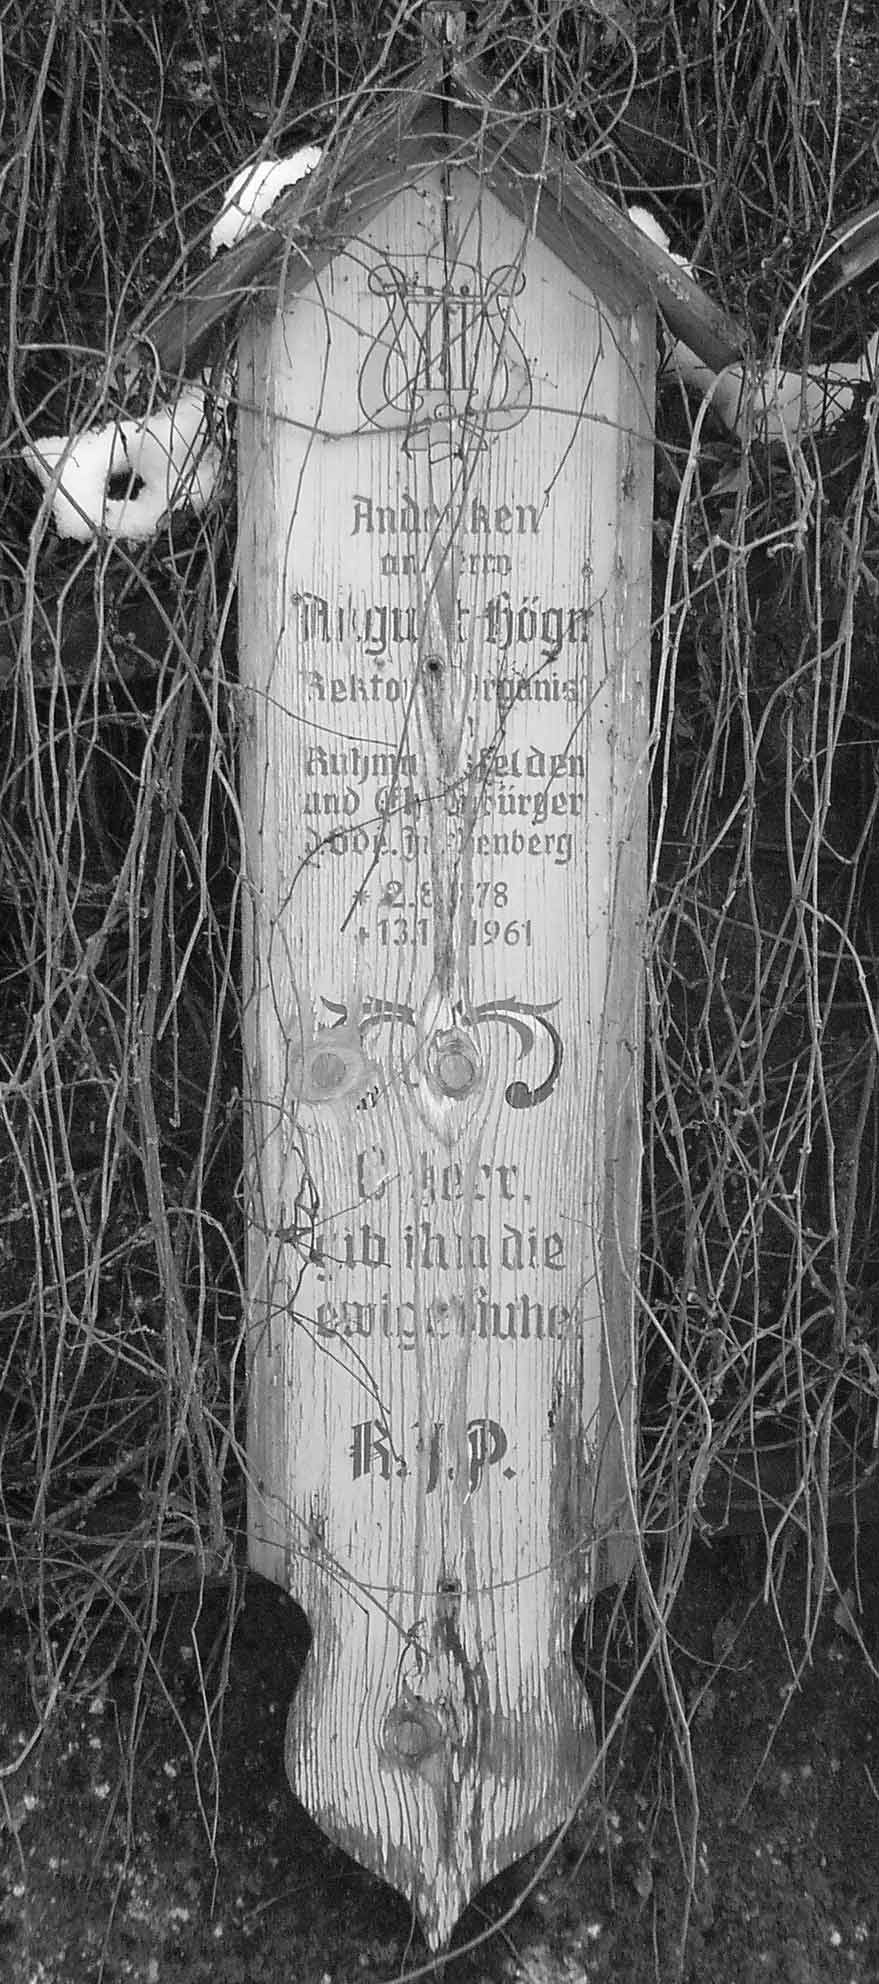
\includegraphics[width=3.51cm,height=7.978cm]{pictures/zulassungsarbeit-img058.jpg}

Abb. \stepcounter{Abb}{\theAbb}: Totenbrett zum Andenken von August Högn
an der Wallfahrtskirche Osterbrünnl in Ruhmannsfelden\\
\end{supertabular}
\end{flushleft}


\section{Werk}
\hypertarget{RefHeadingToc100333739}{}\subsection{Werkverzeichnis}
\label{bkm:Ref99364830}\hypertarget{RefHeadingToc100333740}{}\label{bkm:Ref99368924}\subparagraph{Geistliche
Musik}
\begin{flushleft}
\tablefirsthead{}
\tablehead{}
\tabletail{}
\tablelasttail{}
\begin{supertabular}{m{7.6850004cm}m{8.178cm}}
\multicolumn{2}{m{16.063cm}}{{\bfseries Messen}}\\
\textbf{{\textquotedbl}Laurentius{\textquotedbl}-Messe C-Dur op. 14} &
4-st. gem. Chor, Blechbläserquartett, Orgel\\
{\bfseries {\textquotedbl}Mater-Dei{\textquotedbl}-Messe F-Dur op. 16} &
4-st. gem. Chor, Streichquintett, Orgel\\
\textbf{{\textquotedbl}Josephi{\textquotedbl}-Messe F-Dur op. 62} &
4-st. gem. Chor, Soli, 2 Vl., Blechblquat., Orgel\\
\multicolumn{2}{m{16.063cm}}{{\bfseries Tantum ergo}}\\
{\bfseries 4 Tantum ergo op. 32} &
\\
\textbf{ Tantum ergo Nr. 1 Es-Dur op. 11 } &
4-st. gem. Chor, Streichquintett, Orgel\\
\textbf{ Tantum ergo Nr. 2 F-Dur op. 32} &
4-st. gem. Chor, Streichquintett, Orgel\\
\textbf{ Tantum ergo Nr. 3 Es-Dur op. 49} &
4-st. gem. Chor , Streichquintett, Orgel\\
\textbf{ Tantum ergo Nr. 4 A-Dur op. 47} &
4-st. gem. Chor, Streichquintett, Orgel\\
\multicolumn{2}{m{16.063cm}}{{\bfseries Pange lingua}}\\
\textbf{Pange lingua G-Dur }(deutsch) &
4-st. gem. Chor, Blechbläserquartett\\
{\bfseries Pange lingua F-Dur op. 43 } &
4-st. gem. Chor, Orgel\\
{\bfseries Pange lingua Es-Dur op. 46 } &
4-st. gem. Chor, Orgel\\
{\bfseries Pange lingua Es-Dur op. 51 } &
4-st. gem. Chor, Orgel\\
\multicolumn{2}{m{16.063cm}}{{\bfseries Marienlieder}}\\
{\bfseries Ave Maria F-Dur op. 4} &
Unter- und Oberstimme, Orgel\\
{\bfseries Lieder zum Lobe und Preise Mariens} &
\\
\textbf{ Marienlied Nr. 1 F-Dur op. 13 a } &
4-st. gem. Chor, Orgel\\
\textbf{ Marienlied Nr. 2 e-moll op. 19 } &
Sopran-Solo, 4-st. gem. Chor, Orgel\\
\textbf{ Marienlied Nr. 3 F-Dur op. 22 } &
Sopran-Solo, 4-st. gem. Chor, Orgel\\
\textbf{ Marienlied Nr. 4 G-Dur op. 23 } &
Sopran-Solo, 4-st. gem. Chor, Orgel\\
\textbf{ Marienlied Nr. 5 F-Dur op. 28 } &
4-st. gem. Chor, Orgel\\
\textbf{ Marienlied Nr. 6 F-Dur op. 41 } &
4-st. Frauenchor, Orgel\\
\textbf{ Marienlied Nr. 7 G-Dur op. 45 }(fragmentarisch) &
Sopran-Solo, 4-st. gem. Chor, Orgel\\
\textbf{ Marienlied Nr. 8 G-Dur op. 54} &
Sopran-Solo, 4-st. gem. Chor, Orgel\\
\textbf{ Marienlied Nr. 9 G-Dur op. 34} &
4-st. Männerchor\\
\textbf{ Marienlied Nr. 10 F-Dur op. 56 } &
2 Sopran- und Alt-Solo, 4-st. gem. Chor, Orgel\\
\textbf{ Marienlied Nr. 11 F-Dur op. 59} &
Bariton-Solo, 4-st. gem. Chor, Orgel\\
\textbf{ Marienlied Nr. 12 F-Dur op. 63} &
Sopran- und Alt-Solo, Orgel\\
\textbf{ Marienlied (Nr. 13) C-Dur} &
Sopran-Solo, Klavier o. Harmonium\\
\multicolumn{2}{m{16.063cm}}{{\bfseries Grablieder}}\\
\textbf{Grablied für gefallene Soldaten Es-Dur op. 35} &
4-st. gem. Chor, Blechbläserquartett\\
{\bfseries Grablieder op. 35} &
\\
\textbf{ Grablied Nr. 1 Es-Dur op. 35 } &
4-st. gem. Chor, Blechbläserquartett\\
\textbf{ Grablied Nr. 2 Es-Dur} &
4-st. gem. Chor, Blechbläserquartett\\
\textbf{ Grablied Nr. 3 Es-Dur op. 44} &
4-st. gem. Chor, Blechbläserquartett\\
\textbf{ Grablied Nr. 4 F-Dur op. 20 } &
Sopran-Solo, 4-st. gem. Chor, Orgel\\
\multicolumn{2}{m{16.063cm}}{{\bfseries Offertorien}}\\
{\bfseries Offertorium D-Dur op. 26 } &
4-st. gem. Chor, Orgel\\
{\bfseries Offertorium C-Dur op. 30 } &
4-st. gem. Chor, Orgel\\
{\bfseries Offertorium G-Dur op. 48 } &
4-st. Männerchor, Orgel\\
\multicolumn{2}{m{16.063cm}}{{\bfseries Kommunionlieder}}\\
{\bfseries Kommunionlied Es-Dur op. 12} &
4-st. gem. Chor, Orgel\\
{\bfseries Kommunionlied G-Dur op. 21 a} &
4-st. gem. Chor, Orgel\\
{\bfseries Kommunionlied G-Dur op. 21 b} &
4-st. gem. Chor, Orgel\\
{\bfseries Kommunionlied C-Dur op. 37 b} &
4-st. gem. Chor, Orgel\\
\multicolumn{2}{m{16.063cm}}{{\bfseries Veni creator Spiritius}}\\
{\bfseries Veni creator Spiritus B-Dur} &
4-st. Männerchor\\
{\bfseries 11 Veni creator Spiritus op. 15} &
\\
{\bfseries  Veni creator Spiritus C-Dur Nr. 1} &
4-st. gem. Chor\\
\textbf{ Veni creator Spiritus D-Dur Nr. 2} &
4-st. gem. Chor\\
\textbf{ Veni creator Spiritus Es-Dur Nr. 3} &
4-st. gem. Chor\\
\textbf{ Veni creator Spiritus E-Dur Nr. 4} &
4-st. gem. Chor\\
\textbf{ Veni creator Spiritus F-Dur Nr. 5} &
4-st. gem. Chor\\
\textbf{ Veni creator Spiritus Fis-Dur Nr. 6} &
4-st. gem. Chor\\
\textbf{ Veni creator Spiritus G-Dur Nr. 7} &
4-st. gem. Chor\\
\textbf{ Veni creator Spiritus As-Dur Nr. 8} &
4-st. gem. Chor\\
\textbf{ Veni creator Spiritus A-Dur Nr. 9} &
4-st. gem. Chor\\
{\bfseries  Veni creator Spiritus B-Dur Nr. 10} &
4-st. gem. Chor\\
\textbf{ Veni creator Spiritus H-Dur Nr. 11} &
4-st. gem. Chor\\
\multicolumn{2}{m{16.063cm}}{{\bfseries Adjuva nos}}\\
{\bfseries Adjuva nos Es-Dur op. 8 } &
4-st. gem. Chor, Streichquintett, Orgel\\
{\bfseries 8 Adjuva nos op. 15} &
\\
{\bfseries  Adjuva nos C-Dur Nr. 1} &
4-st. gem. Chor\\
{\bfseries  Adjuva nos D-Dur Nr. 2} &
4-st. gem. Chor\\
\textbf{ Adjuva nos Es-Dur Nr. 3} &
4-st. gem. Chor\\
\textbf{ Adjuva nos E-Dur Nr. 4} &
4-st. gem. Chor\\
\textbf{ Adjuva nos F-Dur Nr. 5} &
4-st. gem. Chor\\
\textbf{ Adjuva nos G-Dur Nr. 6} &
4-st. gem. Chor\\
\textbf{ Adjuva nos A-Dur Nr. 7} &
4-st. gem. Chor\\
\textbf{ Adjuva nos B-Dur Nr. 8} &
4-st. gem. Chor\\
\multicolumn{2}{m{16.063cm}}{{\bfseries verschiedene Genre}}\\
{\bfseries Cäcilienlied E-Dur op. 12 b} &
3-st. Frauenchor, Orgel\\
{\bfseries Libera e-moll op. 50} &
4-st. gem. Chor\\
{\bfseries Benedictus G-Dur op. 50} &
4-st. gem. Chor\\
{\bfseries Fronleichnams-Prozessionsgesänge Es-Dur op. 52} &
4-st. gem. Chor, Blechbläserquartett\\
{\bfseries Ecce sacerdos F-Dur op. 57} &
4-st. gem. Chor, Blechbläserquartett, Orgel\\
{\bfseries Juravit Dominus B-Dur op. 58} &
4-st. gem. Chor, Blechbläserquartett, Orgel\\
{\bfseries {\textquotedbl}Ehre sei Gott{\textquotedbl} C-Dur} &
4-st. gem. Chor\\
\textbf{\textit{Herz-Jesu-Litanei }}\textit{(verloren)} &
\\
\end{supertabular}
\end{flushleft}
\subparagraph{Weltliche Musik}
\begin{flushleft}
\tablefirsthead{}
\tablehead{}
\tabletail{}
\tablelasttail{}
\begin{supertabular}{m{7.6850004cm}m{6.642cm}}
\textbf{Marsch {\textquotedbl}In Treue fest!{\textquotedbl} D-Dur } &
Klavier\\
\textbf{Weihegesang Es-Dur }(fragmentarisch) &
4-st. gem. Chor, Blechbläserquartett\\
\textbf{Lied von Gotteszell G-Dur op. 42 }(Arrangement) &
4-st. Männerchor\\
\end{supertabular}
\end{flushleft}
\clearpage\subparagraph[Arrangements]{Arrangements}
\label{bkm:Ref100328080}\begin{flushleft}
\tablefirsthead{}
\tablehead{}
\tabletail{}
\tablelasttail{}
\begin{supertabular}{m{2.848cm}m{7.743cm}m{5.072cm}}
\multicolumn{3}{m{16.063cm}}{{\bfseries Messen}}\\
Schubert, F.  &
{\bfseries Deutsche Messe Es-Dur} &
für 4-st. gem. Chor arrangiert\\
Siebzehnriegel, F. X.  &
{\bfseries Messe zu Ehren der liebreichen Mutter Es-Dur op. 4} &
Bläserquartett hinzugefügt\\
Stein, J.  &
{\bfseries Instrumental-Messe Nr. 6 Es-Dur op. 78} &
Bläserquartett hinzugefügt\\
\multicolumn{3}{m{16.063cm}}{{\bfseries Requiem}}\\
Deschermeier, J.  &
{\bfseries Missa de Requiem Es-Dur op. 90} &
Bläserquartett hinzugefügt\\
Ett, C.  &
{\bfseries Missa pro defunctis Es-Dur} &
Bläserquartett hinzugefügt\\
Gloger, J.  &
{\bfseries Requiem (Missa IV) d-moll op. 27} &
Bläserquartett hinzugefügt\\
Gruber, J.  &
{\bfseries Missa pro defunctis Es-Dur op. 80} &
Bläserquartett hinzugefügt\\
Gruber, J.  &
{\bfseries Requiem in c-moll op. 114} &
Bläserquartett hinzugefügt\\
Huber, H.  &
{\bfseries Requiem mit Libera c-moll op. 21} &
Bläserquartett hinzugefügt\\
Mitterer, I.  &
{\bfseries Missa pro defunctis As-Dur} &
Bläserquartett hinzugefügt\\
\multicolumn{3}{m{16.063cm}}{{\bfseries Tantum ergo}}\\
Bruckner, A.  &
{\bfseries 6 Tantum ergo As-Dur} &
Violinstimmen hinzugefügt\\
\multicolumn{3}{m{16.063cm}}{{\bfseries Pange lingua}}\\
Goller, V.  &
{\bfseries 12 Pange lingua B-Dur op. 5} &
Bläserquartett hinzugefügt\\
\multicolumn{3}{m{16.063cm}}{{\bfseries Marienlieder}}\\
Griesbacher, P.  &
{\bfseries Marienlied {\textquotedbl}O Himmelskönigin{\textquotedbl}
F-Dur op. 137} &
für Solo und 4-st. gem. Chor arrangiert\\
Griesbacher, P.  &
\textbf{Marienlied {\textquotedbl}Wenn mein Schifflein sich will
wenden{\textquotedbl} C-Dur op. 137} &
für Solo und 4-st. gem. Chor arrangiert\\
Hämel, A.  &
\textbf{Marienlied {\textquotedbl}Ein Bildnis ist mir ins Herz
gegraben{\textquotedbl} F-Dur op. 88} &
für 4-st. gem. Chor arrangiert\\
Schächtl, G.  &
{\bfseries Marienlied {\textquotedbl}Maria, lilienreine!{\textquotedbl}
As-Dur op. 2} &
für 4-st. gem. Chor arrangiert\\
\multicolumn{3}{m{16.063cm}}{{\bfseries Trauungslieder}}\\
Lützel, H.  &
{\bfseries Trauungslied {\textquotedbl}Wo du hingehst{\textquotedbl}
Es-Dur} &
für 4-st. gem. Chor arrangiert\\
Silcher, F.  &
\textbf{Trauungslied {\textquotedbl}So nimm denn meine
Hände{\textquotedbl} D-Dur} &
für 4-st. gem. Chor arrangiert\\
\multicolumn{3}{m{16.063cm}}{{\bfseries Grablieder}}\\
Abt, F. W.  &
{\bfseries Grablied {\textquotedbl}Über den Sternen{\textquotedbl} F-Dur
op. 374 Nr. 3} &
für 4-st. gem. Chor arrangiert\\
Braun, A.  &
{\bfseries Grablied Nr. 7 {\textquotedbl}Geht nun hin und grabt mein
Grab{\textquotedbl} B-Dur } &
für 4-st. gem. Chor arrangiert\\
Claudius, G. K.  &
{\bfseries Grablied Nr. 6 {\textquotedbl}Im Grabe ist Ruh{\textquotedbl}
G-Dur } &
für 4-st. gem. Chor arrangiert\\
Donderer, O.  &
{\bfseries Grablied am Grabe eines Helden Es-Dur op. 1} &
Bläserquartett hinzugefügt\\
Engelhart, F. X.  &
\textbf{Trauerlied {\textquotedbl}Friedhofsglocken rufen
klagend{\textquotedbl} Es-Dur op. 77} &
Bläserquartett hinzugefügt\\
Güttler, J.  &
{\bfseries Grablied Nr. 1 {\textquotedbl}Wie war so mild{\textquotedbl}
Es-Dur} &
Bläserquartett hinzugefügt\\
Güttler, J.  &
{\bfseries Grablied Nr. 2 F-Dur} &
Bläserquartett hinzugefügt\\
Güttler, J.  &
\textbf{Grablied Nr. 3 {\textquotedbl}Das liebe treue
Mutterherz{\textquotedbl} Es-Dur} &
Bläserquartett hinzugefügt\\
Haunschild, F.  &
\textbf{Grablied {\textquotedbl}Treues Herz, nun ruh in
Frieden{\textquotedbl} F-Dur} &
Bläserquartett hinzugefügt\\
Kindsmüller, K.  &
{\bfseries Trauerlied für gefallene Helden F-Dur op. 70} &
Bläserquartett hinzugefügt\\
Pleyer, E.  &
{\bfseries Grablied B-Dur op. 50 Nr. 5} &
Bläserquartett hinzugefügt\\
Schröder, F.  &
\textbf{Zum Gedächtnis unserer gefallenen Krieger Es-Dur} &
Bläserquartett hinzugefügt\\
Seitz, F.  &
\textbf{3 Grabgesänge für gef. Krieger F-Dur op. 28} &
Bläserquartett hinzugefügt\\
Tresch, J. B.  &
{\bfseries Am Grabe eines Kriegers Es-Dur} &
für 4-st. gem. Chor arrangiert, Bläserquartett hinzugefügt\\
\multicolumn{3}{m{16.063cm}}{{\bfseries Offertorien}}\\
Goller, V.  &
{\bfseries Offertorium {\textquotedbl}Terra tremuit{\textquotedbl} B-Dur
op. 22 Nr. 23} &
Bläserquartett hinzugefügt\\
Goller, V.  &
{\bfseries Offertorium {\textquotedbl}Tui sunt coeli{\textquotedbl}
C-Dur op. 21 Nr. 8} &
Bläserquartett hinzugefügt\\
Mitterer, I.  &
{\bfseries Festoffertorien C-Dur op. 89} &
Streichquintett hinzugefügt\\
\multicolumn{3}{m{16.063cm}}{{\bfseries Oster-Liturgie}}\\
Schächtl, G.  &
{\bfseries Deutscher Auferstehungs-Chor Es-Dur op. 24} &
Bläserquartett hinzugefügt\\
\multicolumn{3}{m{16.063cm}}{{\bfseries Herz-Jesu-Lieder}}\\
Griesbacher, P.  &
\textbf{Herz-Jesu-Lied {\textquotedbl}O hätt ich tausend
Herzen{\textquotedbl} D-Dur op. 33 Nr. 2} &
für 4-st. gem. Chor arrangiert\\
Griesbacher, P.  &
\textbf{Herz-Jesu-Lied {\textquotedbl}Dem Herzen Jesu
singe{\textquotedbl} C-Dur op. 33 Nr. 1} &
für 4-st. gem. Chor arrangiert\\
Zangl, J. G.  &
\textbf{Herz-Jesu-Lied {\textquotedbl}Ein Herz hab ich
gefunden{\textquotedbl} G-Dur op. 41 Nr. 1} &
Orgelstimme hinzugefügt\\
Zangl, J. G.  &
{\bfseries Herz-Jesu-Lied {\textquotedbl}O Jesus meine Liebe, zieh
gnädig meinen Sinn{\textquotedbl} As-Dur op. 41 Nr. 2}

 &
Orgelstimme hinzugefügt\\
\end{supertabular}
\end{flushleft}
\begin{center}
\tablefirsthead{}
\tablehead{}
\tabletail{}
\tablelasttail{}
\begin{supertabular}{m{9.701cm}}

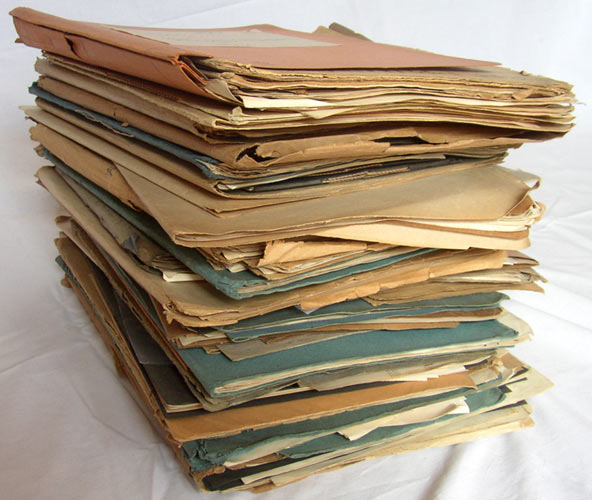
\includegraphics[width=9.491cm,height=8.017cm]{pictures/zulassungsarbeit-img059.jpg}

Abb. \stepcounter{Abb}{\theAbb}: Alle Autographen der Kompositionen von
Högn\\
\end{supertabular}
\end{center}
\clearpage\subparagraph{Anmerkungen zu den Opuszahlen}
Nur als chaotisch kann der Eindruck beschrieben werden, den die
Opuszahlen von Högns Werk auf den Leser machen. Eigentlich sind die
Opuszahlen dafür gedacht, nacheinander im Druck erschienenen Werken
eine fortlaufende Erkennungsnummer zu geben. Da nur der Marsch „In
Treue fest!“ gedruckt wurde, fällt den Nummern bei Högn die Funktion
zu, nacheinander entstandene Werke zu kennzeichnen. Für Verwirrung
sorgen deshalb die vielen doppelten Nummern. So tragen jeweils zwei als
eigenständig anzusehende Werke die Opuszahl 12, 15, 21 und 50. Ebenso
ungewöhnlich erscheint Högns Vorgehensweise, dass er nachträglich
mehrere Werke, die bereits verschiedene Opuszahlen tragen, zu einem
übergeordneten Werkkomplex mit einer neuer Opuszahl zusammenfasste. Die
Komposition „4 Tantum ergo op. 32“ setzt sich etwa aus Stücken mit den
Opusnummern 11, 32, 47 und 49 zusammen. Darüber hinaus passen die 8
Werke ohne Opuszahl nicht recht ins Bild der ansonsten sehr großzügigen
„Opusvergabepraxis.“ Mit dem Lied von Gotteszell G-Dur op. 42 wurde
sogar ein Arrangement gewissermaßen durch die Aufnahme ins Opus
„geadelt“, während hingegen Werke mit weit größerer kompositorischer
Eigenleistung, wie beispielsweise das Grablied Nr. 2 Es-Dur,
unberücksichtig blieben.

\begin{center}
\begin{minipage}{9.241cm}
\begin{center}
\tablefirsthead{}
\tablehead{}
\tabletail{}
\tablelasttail{}
\begin{supertabular}{m{4.5470004cm}m{4.294cm}}

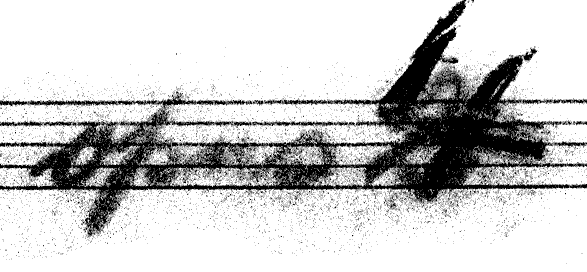
\includegraphics[width=4.364cm,height=2.007cm]{pictures/zulassungsarbeit-img060.png}

Abb. \stepcounter{Abb}{\theAbb}: ausgebesserte Opuszahl auf dem
Autographen des Ave Marias F-Dur op. 4 &

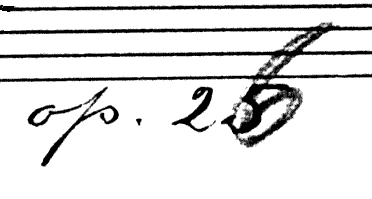
\includegraphics[width=3.739cm,height=2cm]{pictures/zulassungsarbeit-img061.png}

Abb. \stepcounter{Abb}{\theAbb}: ausgebesserte Opuszahl auf dem
Autographen des Offertoriums D-Dur op. 26\\
\end{supertabular}
\end{center}
\end{minipage}
\end{center}
Normalerweise wäre Nummerierung der Werke mit Opuszahlen eine
zuverlässige Informationsquelle bezüglich der Vollständigkeit (siehe
\ref{bkm:Ref98427627} „Zur Frage der Vollständigkeit“, Seite
\pageref{bkm:Ref98427627}) und zeitlichen Entstehung der Kompositionen
(siehe \ref{bkm:Ref98427747} „Entstehungszeit“, Seite
\pageref{bkm:Ref98427747}). Wie können diese Unregelmäßigkeiten erklärt
werden und lassen sich angesichts dieser Unregelmäßigkeiten derartige
Aussagen, wie oben aufgeführt, in Bezug auf Högns Kompositionen machen?

Eine Antwort auf diese Fragen liefert uns die Erörterung der Umstände,
weshalb Högn die offenkundigen Fehler bei der fortlaufenden
Nummerierung unterlaufen sind. Wie man an den Autographen deutlich
erkennen kann, wurden die Opusnummern bis op. 50 nachträglich
hinzugefügt. Högn hatte offensichtlich schon eine Nummerierung seiner
bis dahin geschriebenen Kompositionen in der zeitlichen Abfolge ihrer
Entstehung durchgeführt, als ihm weitere, in der Nummerierung noch
unberücksichtigte Werke unterkamen. Um die Chronologie nicht zu
unterbrechen, entschied er sich, die Opusnummern derjenigen Werke zu
verdoppeln, die nacheinander entstanden waren.

Die Reihenfolge die Opusnummern spiegelt trotz einiger doppelter Nummern
exakt die zeitliche Reihenfolge die Kompositionen wieder. Hätte die
Nummerierung nicht den Sinn gehabt, eine zeitliche Abfolge
herzustellen, sondern die einzelnen Werke besser identifizieren zu
können, wäre es sinnlos gewesen, Nummern zu verdoppeln. Stattdessen
hätte Högn die nächst höhere, noch nicht vergebene Zahl wählen können,
um das noch nicht eingeordnete Werk mit einer eindeutigen
Identifikationsnummer zu belegen. Gruppierungen zu größeren
Werkeinheiten mit neuer Opuszahl, obwohl den untergeordneten Werken
schon Opusnummern vergeben worden sind, stiften zwar etwas Verwirrung,
rütteln aber nicht an der Aussagekraft der untergeordneten Opuszahl,
bezüglich der Entstehungszeit der einzelnen Werke.

Die Existenz der doppelten Nummern, relativiert dagegen die Aussagekraft
der Opuszahlen in Hinblick auf die Frage der Vollständigkeit der Werke
erheblich. Es ist nicht abzusehen, wie viele verschollene Werke mit
gleicher Opuszahl eine Lücke im vorliegenden Werkverzeichnis
geschlossen hätten.

Die Tatsache, dass es doppelte Opuszahlen gibt, kann auch in der
Erklärung, weshalb einige Werke keine Opusnummer tragen,
Richtungweisend sein. Ist es nicht unlogisch, dass Högn einerseits
durch doppelte Opuszahlen „gewaltsam“ versuchte, Werke nachträglich ins
Opus hereinzunehmen und dadurch ein unübersichtliches Bild seines
Gesamtwerks erzeugt, anderseits mancher nicht weniger wertvollen
Komposition eine Opuszahl verwehrt? Viel einleuchtender ist es deshalb,
dass diese Werke mit wenigen Ausnahmen ursprünglich sehr wohl eine
Opuszahl trugen. Wie an den erhaltenen Autographen zu sehen ist, hatte
Högn nur in den seltensten Fällen an alle Bestandteile seines
handgeschriebenen Notenmaterials Opusnummern vermerkt.
Höchstwahrscheinlich sind deshalb bei den Werken ohne Opuszahl nur die
unnummerierten Bestandteile erhalten. Die folgende Tabelle soll bei
jedem einzelnen Werk das Fehlen der Opuszahl begründen und außerdem
eine Vermutung liefern, welche Opuszahl dieses Werk ursprünglich
getragen haben könnte:

\clearpage\begin{flushleft}
\tablefirsthead{}
\tablehead{}
\tabletail{}
\tablelasttail{}
\begin{supertabular}{|m{4.991cm}|m{1.5519999cm}|m{9.12cm}|}
\hline
\textbf{Werk ohne Opusnr.} &
\textbf{Mögl. Opusnr. } &
{\bfseries Begründung für das/die}\\\hline
Marsch {\textquotedbl}In Treue fest!{\textquotedbl} D-Dur  &
1 &
\textbf{Fehlen: }Drucklegung des Marsches vor der Nummerierung

\textbf{Vermutung:} Erstes gedrucktes Werk\\\hline
Grablied Nr. 2 Es-Dur &
36, 38,

39, 40 &
\textbf{Fehlen:} Verlorene Autographen, an denen die Opusnummer vermerkt
war

\textbf{Vermutung:} Fehlende Opuszahlen zwischen Grablied Nr. 1 op. 35
und Grablied Nr. 3 op. 44\\\hline
Herz-Jesu-Litanei &
53, 55,

60, 61 &
\textbf{Fehlen:} Werk ist komplett verschollen

\textbf{Vermutung:} Titel bekannt aus Briefen des Jahres 1948,
wahrscheinlich daher späte Entstehung \\\hline
{\textquotedbl}Ehre sei Gott{\textquotedbl} C-Dur &
53, 55,

60, 61 &
\textbf{Fehlen:} Verlorene Autographen, an denen die Opusnummer vermerkt
war

\textbf{Vermutung:} Deutscher Text, daher Entstehung im Vorfeld des II.
Vatikanischen Konzils, wahrscheinlich deswegen späte Entstehungszeit
\\\hline
Pange lingua (deutsch) G-Dur &
53, 55,

60, 61 &
\textbf{Fehlen:} Verlorene Autographen, an denen die Opusnummer vermerkt
war

\textbf{Vermutung:} Deutscher Text, daher Entstehung im Vorfeld des II.
Vatikanischen Konzils, wahrscheinlich deswegen späte Entstehungszeit ab
45 \\\hline
Marienlied (Nr. 13) C-Dur

 &
64 &
\textbf{Fehlen:} Verlorene Autographen, an denen die Opusnummer vermerkt
war

\textbf{Vermutung:} Letzte erhaltene Komposition\\\hline
Veni creator Spiritus B-Dur &
{}- &
\textbf{Fehlen:} Frühe Version des Veni creator Spiritus D-Dur op. 15
Nr. 2\\\hline
Weihegesang Es-Dur &
{}- &
\textbf{Fehlen:} Verworfen bevor Nummerierung durchgeführt wurde
(NS-Musik)\\\hline
\end{supertabular}
\end{flushleft}
\subsubsection{Zur Frage der Vollständigkeit des Werkverzeichnisses}
\label{bkm:Ref98427627}\hypertarget{RefHeadingToc100333741}{}Die 24
Lücken (grau markiert) in dem 63 Opusnummern umfassenden Werk von Högn
machen eines deutlich: Es sind nicht alle Kompositionen erhalten. An
dieser Stelle sollte deshalb neben den Gründen, für den Verlust einiger
seiner Kompositionen besonders die Fragen nach Anzahl und Art der nicht
erhaltenen Kompositionen in den Mittelpunkt gestellt werden.

\begin{center}
\begin{minipage}{8.096cm}
\begin{flushleft}
\tablefirsthead{}
\tablehead{}
\tabletail{}
\tablelasttail{}
\begin{supertabular}{|m{0.60800004cm}|m{0.60800004cm}|m{0.60800004cm}|m{0.60800004cm}|m{0.60800004cm}|m{0.60800004cm}|m{0.60800004cm}|m{0.60800004cm}|m{0.60800004cm}|m{0.626cm}|}
\hline
\begin{enumerate}
\item
\end{enumerate}
 &
\begin{enumerate}
\item
\end{enumerate}
 &
\begin{enumerate}
\item
\end{enumerate}
 &
\begin{enumerate}
\item
\end{enumerate}
 &
\begin{enumerate}
\item
\end{enumerate}
 &
\begin{enumerate}
\item
\end{enumerate}
 &
\begin{enumerate}
\item
\end{enumerate}
 &
\begin{enumerate}
\item
\end{enumerate}
 &
\begin{enumerate}
\item
\end{enumerate}
 &
\begin{enumerate}
\item
\end{enumerate}
\\\hline
\begin{enumerate}
\item
\end{enumerate}
 &
\begin{enumerate}
\item
\end{enumerate}
 &
\begin{enumerate}
\item
\end{enumerate}
 &
\begin{enumerate}
\item
\end{enumerate}
 &
\begin{enumerate}
\item
\end{enumerate}
 &
\begin{enumerate}
\item
\end{enumerate}
 &
\begin{enumerate}
\item
\end{enumerate}
 &
\begin{enumerate}
\item
\end{enumerate}
 &
\begin{enumerate}
\item
\end{enumerate}
 &
\begin{enumerate}
\item
\end{enumerate}
\\\hline
\begin{enumerate}
\item
\end{enumerate}
 &
\begin{enumerate}
\item
\end{enumerate}
 &
\begin{enumerate}
\item
\end{enumerate}
 &
\begin{enumerate}
\item
\end{enumerate}
 &
\begin{enumerate}
\item
\end{enumerate}
 &
\begin{enumerate}
\item
\end{enumerate}
 &
\begin{enumerate}
\item
\end{enumerate}
 &
\begin{enumerate}
\item
\end{enumerate}
 &
\begin{enumerate}
\item
\end{enumerate}
 &
\begin{enumerate}
\item
\end{enumerate}
\\\hline
\begin{enumerate}
\item
\end{enumerate}
 &
\begin{enumerate}
\item
\end{enumerate}
 &
\begin{enumerate}
\item
\end{enumerate}
 &
\begin{enumerate}
\item
\end{enumerate}
 &
\begin{enumerate}
\item
\end{enumerate}
 &
\begin{enumerate}
\item
\end{enumerate}
 &
\begin{enumerate}
\item
\end{enumerate}
 &
\begin{enumerate}
\item
\end{enumerate}
 &
\begin{enumerate}
\item
\end{enumerate}
 &
\begin{enumerate}
\item
\end{enumerate}
\\\hline
\begin{enumerate}
\item
\end{enumerate}
 &
\begin{enumerate}
\item
\end{enumerate}
 &
\begin{enumerate}
\item
\end{enumerate}
 &
\begin{enumerate}
\item
\end{enumerate}
 &
\begin{enumerate}
\item
\end{enumerate}
 &
\begin{enumerate}
\item
\end{enumerate}
 &
\begin{enumerate}
\item
\end{enumerate}
 &
\begin{enumerate}
\item
\end{enumerate}
 &
\begin{enumerate}
\item
\end{enumerate}
 &
\begin{enumerate}
\item
\end{enumerate}
\\\hline
\begin{enumerate}
\item
\end{enumerate}
 &
\begin{enumerate}
\item
\end{enumerate}
 &
\begin{enumerate}
\item
\end{enumerate}
 &
\begin{enumerate}
\item
\end{enumerate}
 &
\begin{enumerate}
\item
\end{enumerate}
 &
\begin{enumerate}
\item
\end{enumerate}
 &
\begin{enumerate}
\item
\end{enumerate}
 &
\begin{enumerate}
\item
\end{enumerate}
 &
\begin{enumerate}
\item
\end{enumerate}
 &
\begin{enumerate}
\item
\end{enumerate}
\\\hline
\begin{enumerate}
\item
\end{enumerate}
 &
\begin{enumerate}
\item
\end{enumerate}
 &
\begin{enumerate}
\item
\end{enumerate}
 &
\multicolumn{7}{m{5.474cm}}{}\\\hhline{---~~~~~~~}
\end{supertabular}
\end{flushleft}
\end{minipage}
\end{center}
Der Hauptgrund für das Abhandenkommen einiger von Högns Kompositionen
liegt an den unzureichenden Vorkehrungen zum dauerhaften Erhalt seines
kompositorischen Nachlasses. Nach Högns Tod hatte die Haushälterin Rosa
Beischmied den Auftrag erhalten, sich um die Auflösung seiner Wohnung
zu kümmern. \footnote{Interview Nr. 20, Gertraud von Molo, 23.11.2004,
Absatz 35; Interview Nr. 2, Barbara Essigmann, 27.12.2002, Absatz 76}
Da sämtliche Kompositionen in Ruhmannsfelden verblieben, lag es an der
Haushälterin, ihren weiteren Verwendungszweck zu bestimmen. Allein
schon die vielen verschiedenen Fundorte von Högns Kompositionen
sprechen dafür, dass Beischmied an mehrere Personen beziehungsweise
Institutionen die noch in Högns Wohnung verbliebenen Werke
weitergegeben hatte. Die Fundorte waren im Einzelnen: der Notenschrank
und Dachboden des linken Seitenschiffs der Pfarrkirche St. Laurentius,
der Pfarrhof St. Laurentius, die Wohnung des ehemaligen
Kirchenchorleiters und Leiters des Ruhmannsfeldener Männerchors Franz
Danziger, das Haus der Sängerin Mathilde Glasschröder sowie die
Bayerische Staatsbibliothek, München.

\begin{flushleft}
\tablefirsthead{}
\tablehead{}
\tabletail{}
\tablelasttail{}
\begin{supertabular}{m{3.7419999cm}m{0.8cm}m{4.3cm}m{2.3009999cm}m{4.801cm}}
{\centering   [Warning: Image ignored]
% Unhandled or unsupported graphics:
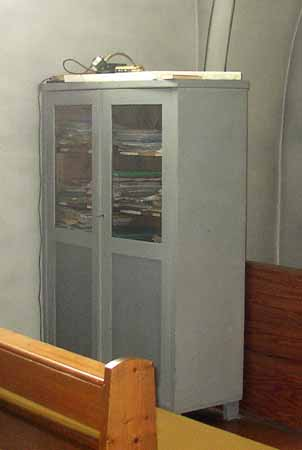
\includegraphics[width=3.674cm,height=5.509cm]{pictures/zulassungsarbeit-img062.jpg}
 \par}
Abb. \stepcounter{Abb}{\theAbb}: Notenschrank der Pfarrkirche St.
Laurentius &
\multicolumn{2}{m{5.3cm}}{{\raggedleft   [Warning: Image ignored]
% Unhandled or unsupported graphics:
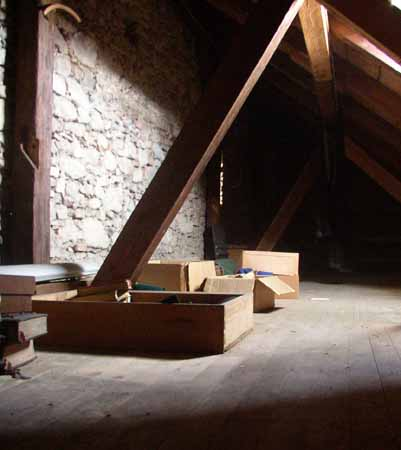
\includegraphics[width=4.951cm,height=5.509cm]{pictures/zulassungsarbeit-img063.jpg}
 \par}
Abb. \stepcounter{Abb}{\theAbb}: Dachboden des linken Seitenschiffs der
Pfarrkirche St. Laurentius} &
\multicolumn{2}{m{7.302cm}}{  [Warning: Image ignored]
% Unhandled or unsupported graphics:
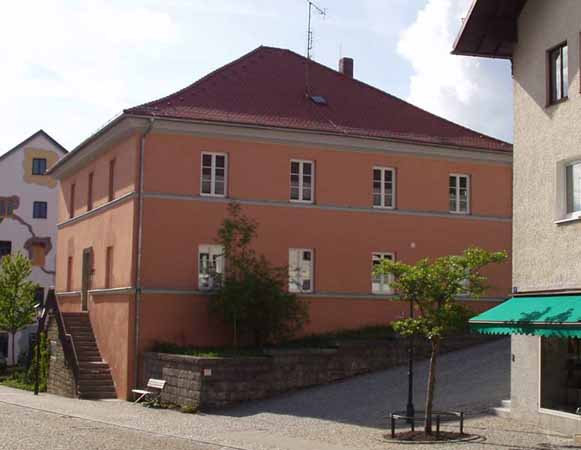
\includegraphics[width=7.091cm,height=5.509cm]{pictures/zulassungsarbeit-img064.jpg}

Abb. \stepcounter{Abb}{\theAbb}: Pfarrhof St. Laurentius,
Ruhmannsfelden}\\
\multicolumn{2}{m{4.742cm}}{  [Warning: Image ignored]
% Unhandled or unsupported graphics:
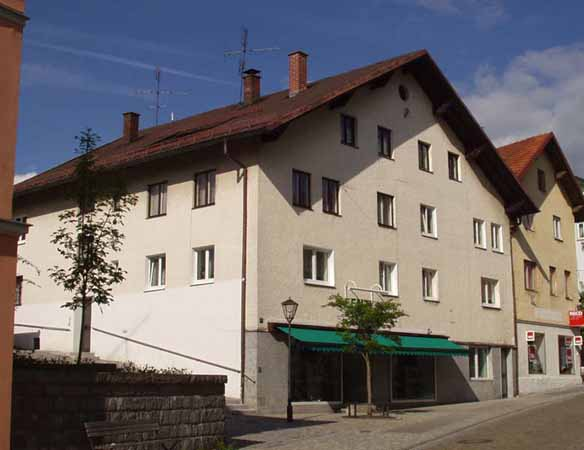
\includegraphics[width=4.531cm,height=3.493cm]{pictures/zulassungsarbeit-img065.jpg}

Abb. \stepcounter{Abb}{\theAbb}: Wohnung von Franz Danziger} &
\multicolumn{2}{m{6.801cm}}{  [Warning: Image ignored]
% Unhandled or unsupported graphics:
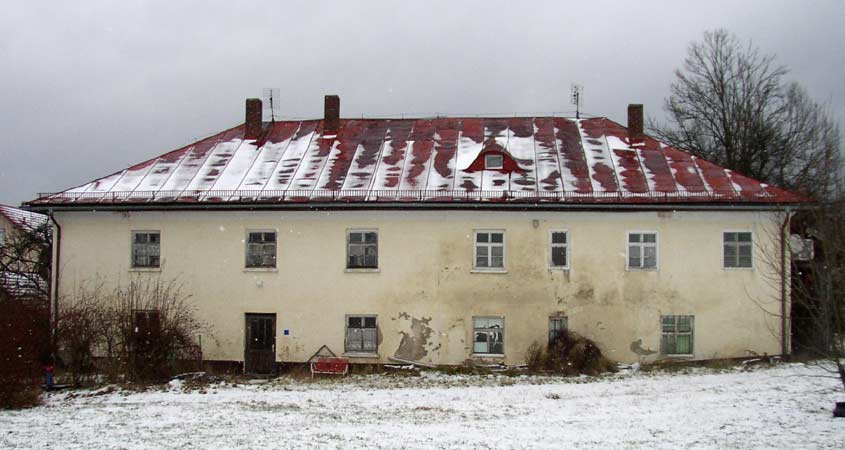
\includegraphics[width=6.549cm,height=3.487cm]{pictures/zulassungsarbeit-img066.jpg}

Abb. \stepcounter{Abb}{\theAbb}: Haus der Sängerin Mathilde
Glasschröder} &

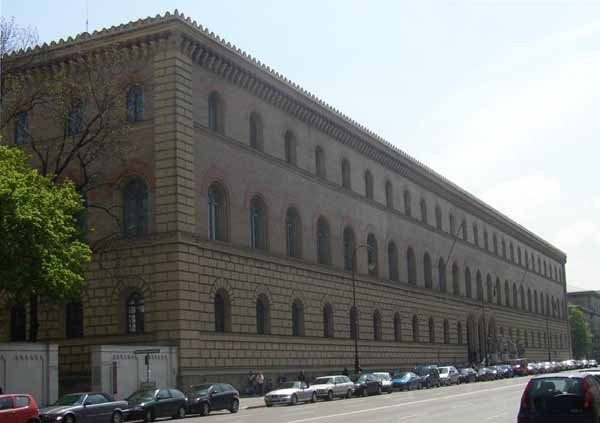
\includegraphics[width=4.509cm,height=3.491cm]{pictures/zulassungsarbeit-img067.jpg}

Abb. \stepcounter{Abb}{\theAbb}: Bayerische Staatsbibliothek\\
\end{supertabular}
\end{flushleft}
Einzeln verstreute, über den ganzen Ort Ruhmannsfelden aufgewahrte Werke
unterliegen weit mehr der Vernichtungsgefahr aus Unwissenheit, als der
in einem Archiv aufbewahrte Bestand des Nachlasses. Es ist daher nicht
verwunderlich, dass es konkrete Anhaltspunkte gibt, wonach
Kompositionen von Högn vernichtet worden sein könnten. Da Franz
Danziger nicht nur Kirchenchorleiter, sondern zur Zeit der Auflösung
von Högns Wohnung auch Leiter des Ruhmannsfeldener Männerchores war und
im Turnverein-Orchester unter Högn mitwirkte, \footnote{Dokument Nr.
56, Auszug aus den Memoiren von Franz Danziger sen., 1984} müsste seine
Wohnung ein weit ergiebigerer Fundort gewesen sein. Hier war aber kein
einziges weltliches Werk neben den entdeckten geistlichen Kompositionen
zum Vorschein gekommen. Der Sohn des ehemaligen Kirchenchorleiters
räumte in seinem Brief vom 25.10.2002 ein, dass seine Mutter bei
Entsorgungsarbeiten eventuell auch Werke von Högn vernichtet haben
könnte. \footnote{Korrespondenz Nr. 7, Brief von Franz Danziger an
Josef Friedrich, 25.10.2002} Es ist anzunehmen, dass selbst zu Högns
Lebzeiten einige seiner Werke eventuell verloren gegangen sind. Nach
der Entlassung von Högn als Chorregent durch Reicheneder haben die
Sängerinnen Barbara Essigmann und Mathilde Glasschröder alle
Kompositionen aus der Kirche mitgenommen und in Högns Wohnung getragen.
Die Haushälterin Rosa Beischmied trug sie kurz darauf wieder
zurück. \footnote{Interview Nr. 2, Barbara Essigmann, 27.12.2002,
Absatz 56} Dass bei diesem „Gezerre“ um die Noten nach Högns Entlassung
das eine oder andere Werk verloren ging, liegt durchaus im Bereich des
Möglichen. Nach Aussage von Barbara Essigmann hat die Sängerin Maria
Schröck weit mehr Kompositionen von Högn als nur die „Josephi“-Messe
ihrem neuem Chorregenten Fritz Goller in Deggendorf (siehe
\ref{bkm:Ref98506951} „„Josephi“-Messe F-Dur op. 62“, Seite
\pageref{bkm:Ref98506963}) übergeben. \footnote{Interview Nr. 2,
Barbara Essigmann, 27.12.2002, Absatz 18} Höchstwahrscheinlich sind
einige von Högns Kompositionen in Deggendorf verloren gegangen, denn
weder im Nachlass von Fritz Goller \footnote{Korrespondenz Nr. 27,
E-Mail von Martina Goller an Josef Friedrich, 4.3.2003} noch in den
Notenbeständen seiner ehemaligen Wirkungsstätten Mariä
Himmelfahrt \footnote{Korrespondenz Nr. 32, E-Mail von Hermann Wellner
an Josef Friedrich, 25.3.2003} und St. Martin konnten Werke von Högn
ausfindig gemacht werden. Da nicht bekannt ist, an wie viele Personen
Rosa Beischmied Kompositionen übergeben hat, ist nicht auszuschließen,
dass noch weitere seiner Werke existieren. Ihr Aufbewahrungsort bleibt
jedoch unbekannt. Weitere mögliche Fundorte wurden deshalb ohne einen
konkreten Hinweis erfolglos. Nachforschungen über den Verbleib von
Kompositionen beim Achslacher Männerchor, den Franz Danziger bis ins
hohe Rentenalter leitete und mit dem er 1983 ein Marienlied von Högn
aufführte, \footnote{Dokument Nr. 74, Zeitungsartikel aus dem
Viechtacher Bayerwald-Boten, 1983} brachten keine positiven
Ergebnisse. \footnote{Korrespondenz Nr. 85, E-Mail von Franz Aichinger
an Josef Friedrich, 4.1.2005} Centa Schwannberger, die Ehefrau von
Rudolf Schwannberger, der zusammen mit Högn die Sängerriege des
Turnvereins leitete, hat den Notenbestand ihres Mannes den
Geißkopfsängern übergeben. Hier verlaufen sich die Spuren.\footnote{
Korrespondenz Nr. 91, Telefonat von Helmut Gärtner an Josef Friedrich,
8.1.2005} Auch die Nachfahren von Vitus Voit, einem Mitwirkenden im
Turnverein-Orchester, konnten keine von Högns Kompositionen finden.

Es stellt sich nun die Frage nach der Anzahl der nicht mehr erhaltenen
Kompositionen von Högn. Da Högns Opuszahlen nur eine sehr
eingeschränkte Aussagekraft in Bezug auf die tatsächlich komponierten
Werke haben (siehe \ref{bkm:Ref99364830} „Anmerkungen zu den
Opuszahlen“, Seite \pageref{bkm:Ref98509933}) und Högn selbst kein
Werkverzeichnis hinterließ, kann keine genaue Zahl verlorener
Kompositionen genannt werden. Das Verhältnis von 24 fehlenden
Opuszahlen zu 50 erhaltenen Werken (39 Werke mit Opuszahl + 4 Werke mit
doppelter Opuszahl + 7 Werke ohne Opuszahl), suggeriert in etwa ein
Verhältnis von 1 zu 2. Demnach kann man die Meinung vertreten, dass
ungefähr zwei Drittel von Högns ursprünglichem Werk erhalten sind.

Einige konkrete Hinweise lassen Rückschlüsse zu, wie sich der unbekannte
Teil seines Werks zusammengesetzt haben könnte. Nur von einer
verschollenen Komposition ist der Namen bekannt. Drei Briefe erwähnen
eine „Herz-Jesu-Litanei.“ Es muss eine bedeutende Komposition gewesen
sein, denn Högn wollte sie sogar drucken lassen.
\footnote{Dokument Nr. 60, Brief von Sebaldus-Verlag, Bamberg an August Högn, 20.5.1947;
Dokument Nr. 59, Brief von Gregorius-Verlag, Regensburg an August Högn, 9.6.1947;
Dokument Nr. 57, Brief von Gregorius-Verlag, Regensburg an August Högn, 16.6.1947}
In Otto
Geyers Buch „Schule und Lehrer in Niederbayern“ ist ein Kapitel den
niederbayerischen Lehrerkomponisten gewidmet. Als eine Gattung von
Högns Werk erwähnt Geyer hier auch Requien. \footnote{Geyer, Seite 95}
Das Libera e-moll op. 50 ist wohl der klägliche Rest von Högns
Requien-Schaffen. Einige Hinweise lassen Rückschlüsse auf Högns
verschollene weltliche Kompositionen zu. An seinem 80. Geburtstag
versprach Högn dem Ruhmannsfeldener Männerchor unter der Leitung von
Franz Danziger \zitat{„weiteres Notenmaterial zur Verfügung
zu stellen.“ } \footnote{Dokument Nr. 49, Zeitungsartikel aus
Viechtacher Bayerwald-Bote, 5.8.1958} Laut Johann Glasschröder, dem
damaligen Vorstand, hat Högn für den Männerchor tatsächlich
komponiert. \footnote{Interview Nr. 24, Johann Glasschröder,
28.12.2004, Absatz 32} Högn hatte neben dem Ruhmannsfeldener Männerchor
noch zu weiteren Männerchören Kontakt. Bei der 1919 gegründeten
Sängerriege des Turnvereins Ruhmannsfelden unter der Leitung von Rudolf
Schwannberger fungierte Högn sogar zeitweise als Dirigent.\footnote{
Dokument Nr. 104, Protokoll der Turnvereinsversammlung, 27.9.1919;
Dokument Nr. 105, Protokoll der Turnvereinsversammlung, 29.12.1919} Das
Marienlied Nr. 9 op. 34 ist eine Auftragskomposition für einen
Männerchor aus Regen. Högn hatte zum Leiter dieses Regener Chores ein
freundschaftliches Verhältnis, wie aus dem im sehr kameradschaftlichen
Ton gehalten Brief an Högn ersichtlich ist. \footnote{Dokument Nr. 62,
Brief von „Franzl“, Regen an August Högn, 17.6.1928} Diese Männerchöre
könnten Gelegenheiten zur Aufführung und daher Anlass zur Entstehung
von Kompositionen geboten haben.

\begin{flushleft}
\tablefirsthead{}
\tablehead{}
\tabletail{}
\tablelasttail{}
\begin{supertabular}{m{2.809cm}}

\begin{center}

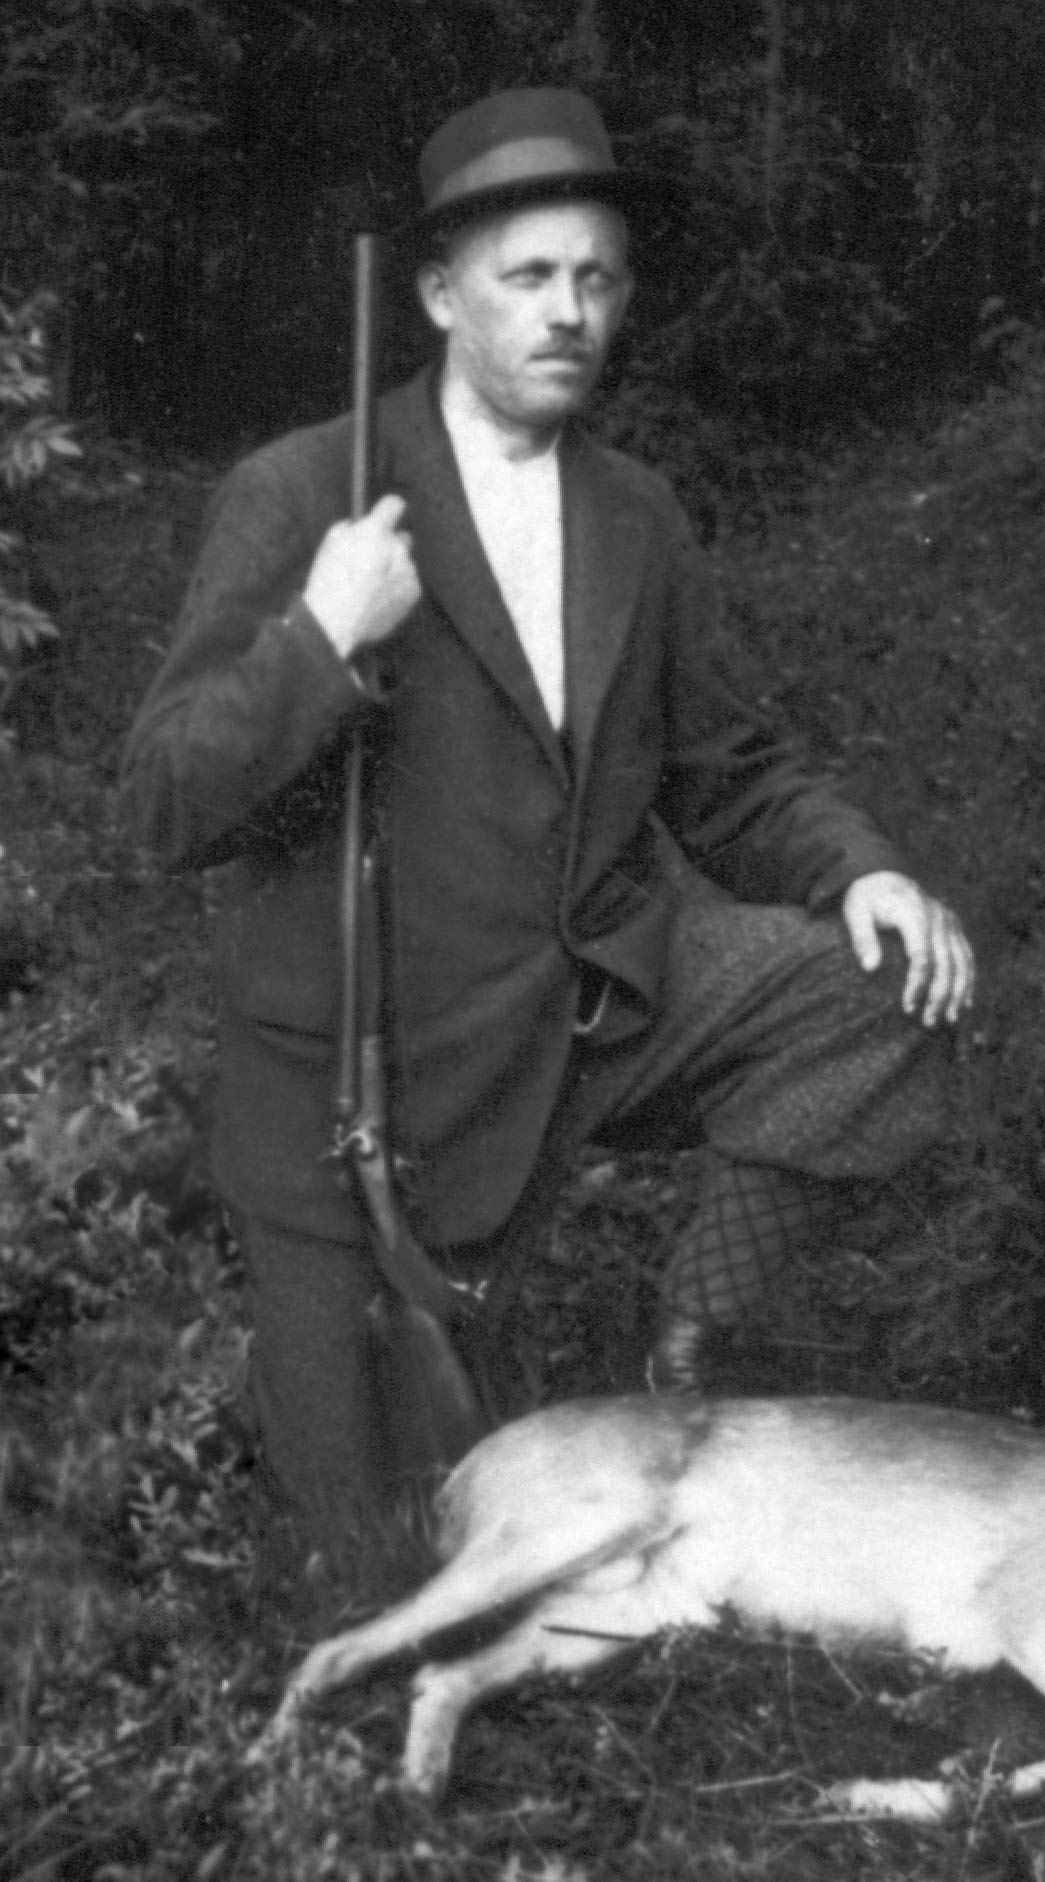
\includegraphics[width=2.626cm,height=4.68cm]{pictures/zulassungsarbeit-img068.jpg}

\end{center}
Abb. \stepcounter{Abb}{\theAbb}: August Högn auf der Jagd\\
\end{supertabular}
\end{flushleft}
Nach Barbara Essigmann lassen sich auch diese weltlichen Chorsätze
thematisch näher bestimmen. Högn, ein begeisterter Jäger, soll viele
„Jägerlieder“ geschrieben haben, die beispielsweise auf einer
Geburtstagsfeier des Kreisjägermeisters und Kirchenchormitgliedes
Rudolf Schwannberger oder in der Schule gesungen wurden.\footnote{
Interview Nr. 5, Barbara Essigmann, 2.1.2003, Absatz 40} Das Fach
Singen in der Schule kann als weiteres kompositorisches Betätigungsfeld
von August Högn angesehen werden. Wenn er nicht eigene Lieder schrieb,
dann fertigte er mit Sicherheit Arrangements für seine Schüler und
Schülerinnen an. \footnote{Interview Nr. 16, Maria Freisinger,
25.8.2004, Absatz 24} Der Satz des Adventliedes „Tauet Himmel“ ist ein
Beispiel dafür. Auf das Notenblatt dieses Arrangements vermerkte Högn:
„Aus meinen Kinderliedern.“ Högn hatte sich anscheinend eine Sammlung
von Liedsätzen für den Schuleinsatz angelegt. Wenn es sich bei diesen
Schulliedern um eine ähnliche Zusammenstellung handelte, wie die
Sammlung der Marienlieder und Grablieder, dann ist davon auszugehen,
dass neben Abschriften und Arrangements auch eigene Kompositionen dazu
gehörten. Högn hat über 30 Marienlieder und 7 Grablieder
zusammengestellt und durchnummeriert. Die ersten 12 Nummern der
Marienlieder und die ersten 4 Nummern der Grablieder stellen eigene
Kompositionen dar, dann folgen Arrangements und Abschriften. Ob Högn
noch mehr an Instrumentalmusik als nur den im Selbstverlag erschienenen
Marsch „In Treue fest!“ hinterlassen hat, darüber kann spekuliert
werden. Normalerweise schreibt ein Komponist mehrere Stücke zu einem
bestimmten Genre, bis er dann das ausgereifteste Werk in Druck gibt.
Und ermuntert nicht eine erschienene Komposition zu weiterer
Kompositionsarbeit am gleichen Genre? Es wäre ebenfalls denkbar, dass
Kompositionen auch für die Orchesterriege des Turnvereins
Ruhmannsfelden entstanden sind, die Högn in den 20er- und 30er-Jahren
des 20. Jahrhunderts leitete.

\subsubsection{Entstehungszeit der Kompositionen}
\label{bkm:Ref98427747}\hypertarget{RefHeadingToc100333742}{}Nur zu ganz
wenigen Kompositionen hat August Högn deren Entstehungszeit notiert. Da
die Opuszahlen die Reihenfolge, wie die einzelnen Kompositionen
nacheinander entstanden sind, zumindest ungefähr wiedergeben (siehe
\ref{bkm:Ref99368924} „Anmerkungen zu den Opuszahlen“, Seite
\pageref{bkm:Ref98509933}), kann man mit den spärlichen Datumsangaben
zumindest zeitliche Bereiche eingrenzen. Informationen aus Högns
Biographie, zeitgeschichtliche Fakten sowie Beobachtungen an den
Handschriften lassen noch weiteren Kompositionen eine nähere Zeitangabe
zuordnen, sodass man die Gruppierung in zeitliche Bereiche
differenzieren kann.

\begin{flushleft}
\tablefirsthead{}
\tablehead{}
\tabletail{}
\tablelasttail{}
\begin{supertabular}{|m{6.242cm}|m{9.621cm}|}
\hline
{\bfseries Werk} &
{\bfseries Entstehungszeit}\\\hline
{\bfseries Veni creator Spiritus B-Dur} &
1897/98\\\hline
{\bfseries Marsch {\textquotedbl}In Treue fest!{\textquotedbl} D-Dur } &
1905\\\hline
{\bfseries Marienlied Nr. 9 G-Dur op. 34 } &
19.6.1928\\\hline
{\bfseries Marienlied Nr. 12 F-Dur op. 63 } &
1. Fastensonntag 1954\\\hline
{\bfseries Marienlied (Nr. 13) C-Dur} &
Laetare 1954 (Text), 300-jähr. Osterbrünnljubiläum 1960 (Musik)\\\hline
\end{supertabular}
\end{flushleft}
Högns op. 11 ist wahrscheinlich zu Beginn seiner ersten Chorregentenzeit
1921 entstanden. Zwischen op. 11 und op. 16 sind alle Kompositionen
vollständig vorhanden, und es handelt sich in diesem Bereich um
ausschließlich geistliche Werke. Die vielen Lücken zwischen op. 1 und
op. 10 – nur zwei Kompositionen aus diesem Bereich waren auffindbar –
lassen sich dadurch erklären, dass Högn in dieser Zeit vor allem
weltliche Musik für die Sänger- und Orchesterriege des Turnvereins
geschrieben hat, die sowie die meisten Stücke seines weltlichen
Schaffens nicht überliefert ist. Die Übernahme des Kirchenchores 1921
machte offenbar eine stark gesteigerte kompositorische Tätigkeit auf
dem Gebiet der Kirchenmusik notwendig. So entstanden in einem seinen
Anfangsjahren als Chorregent ausschließlich kirchenmusikalische Werke.

\begin{flushleft}
\tablefirsthead{}
\tablehead{}
\tabletail{}
\tablelasttail{}
\begin{supertabular}{m{7.9230003cm}m{7.9230003cm}}
\subparagraph{1897 – 1921}
Veni creator Spiritus B-Dur

Marsch {\textquotedbl}In Treue fest!{\textquotedbl} D-Dur

Ave Maria F-Dur op. 4

Adjuva nos Es-Dur op. 8

\subparagraph{1921 – 1928}
Tantum ergo Nr. 1 Es-Dur op. 11

Kommunionlied Es-Dur op. 12

Cäcilienlied E-Dur op. 12 b

Marienlied Nr. 1 F-Dur op. 13 a

{\textquotedbl}Laurentius{\textquotedbl}-Messe C-Dur op. 14

11 Veni creator Spiritus C-Dur op. 15

8 Adjuva nos op. 15

{\textquotedbl}Mater-Dei{\textquotedbl}-Messe F-Dur op. 16

Marienlied Nr. 2 G-Dur op. 19

Grablied Nr. 4 F-Dur op. 20

Kommunionlied G-Dur op. 21 a

Kommunionlied G-Dur op. 21 b

Marienlied Nr. 3 F-Dur op. 22

Marienlied Nr. 4 G-Dur op. 23

Offertorium D-Dur op. 26

Marienlied Nr. 5 F-Dur op. 28

Offertorium C-Dur op. 30

Tantum ergo Nr. 2 F-Dur op. 32

Marienlied Nr. 9 G-Dur op. 34

\subparagraph{1928 – 1939}
{}-{}-{}-{}- Keine Werke -{}-{}-{}-

(Chorregent Albert Schroll) &
\subparagraph{1939 – 1945}
Grablied für gefallene Soldaten Es-Dur op. 35

Grablied Nr. 1 Es-Dur op. 35

Kommunionlied C-Dur op. 37 b

Marienlied Nr. 6 F-Dur op. 41

Lied von Gotteszell G-Dur op. 42

Pange lingua F-Dur op. 43

Grablied Nr. 3 Es-Dur op. 44

Marienlied Nr. 7 G-Dur op. 45

Pange lingua Es-Dur op. 46

Tantum ergo Nr. 4 A-Dur op. 47

Offertorium G-Dur op. 48

Tantum ergo Nr. 3 Es-Dur op. 49

Libera e-moll op. 50

Benedictus G-Dur op. 50

\ \ Grablied Nr. 2 Es-Dur

\ \ Weihegesang Es-Dur

\subparagraph{1945 – 1953}
Pange lingua Es-Dur op. 51

Fronleichnams-Prozessionsgesänge Es-Dur op. 52

Marienlied Nr. 8 G-Dur op. 54

Marienlied Nr. 10 F-Dur op. 56

Ecce sacerdos F-Dur op. 57

Juravit Dominus B-Dur op. 58

Marienlied Nr. 11 F-Dur op. 59

{\textquotedbl}Josephi{\textquotedbl}-Messe F-Dur op. 62

Marienlied Nr. 12 F-Dur op. 63

\ \ Herz-Jesu-Litanei

Pange lingua (deutsch) G-Dur

\ \ {\textquotedbl}Ehre sei Gott{\textquotedbl} C-Dur

\subparagraph{1953 – 1961}
Marienlied (Nr. 13) C-Dur \\
\end{supertabular}
\end{flushleft}
Da der Beginn des 2. Weltkrieges und der Anfang von Högns 3.
Chorregentenzeit zeitlich eng aneinander liegen, dürfte das Grablied
für gefallene Soldaten Es-Dur op. 35 die erste in seiner 3. Phase als
Chorleiter geschriebene Komposition sein. Das würde bedeuten, dass
zwischen dem vorhergehenden Werk mit der Opuszahl 34, das am 19.6.1928
fertig gestellt wurde, also gegen Ende von Högns 2. Chorregentenzeit,
und dem op. 35 ein Zeitraum von über 10 Jahren liegt. Zu dieser Zeit
war Albert Schroll Chorregent.

Werke mit einer größeren Nummer als op. 51 sind vermutlich kurz nach
Ende des 2. Weltkriegs entstanden. Dieser Zeitpunkt liegt einerseits
nahe, wenn man eine regelmäßige Kompositionstätigkeit Högns in seiner
von 1939 bis 1953 andauernden 3. Chorregentenzeit annimmt. Da das op.
51 die erste nicht nachträglich mit einer Opuszahl versehene
Komposition ist, kann man auf der anderen Seite davon ausgehen, dass
das Werk mit der Opuszahl 51 kurz nach Abschluss der nachträglichen
Nummerierungsarbeiten der bisherigen Werke Högns entstanden ist. Es ist
sehr wahrscheinlich, dass diese Nummerierungsarbeiten in der durch die
Entnazifizierung verursachten Zwangspause von 1945 bis 1947
stattfanden, als Högn vom Schuldienst suspendiert wurde und erstmals
Zeit gefunden hatte, sich um die Pflege seiner bisher entstandenen
Kompositionen zu kümmern.

\subsubsection{Herkunft der vertonten Texte}
\hypertarget{RefHeadingToc100333743}{}Nur bei 6 seiner Kompositionen mit
deutschem Text gibt Högn jeweils den entsprechenden Autor an. Die Texte
stammen von Schwester M. Irmingard, Hühnlein, Dr. Anton Götz, Otto
Schaffner, Hans Trohsbach, und Cordula Peregrina. Vier von Högns
Kompositionen haben ihren Text mit Werken aus dem Notenmaterial der
Pfarrei Ruhmannsfelden gemeinsam, wie folgender Tabelle zu entnehmen
ist:

\begin{flushleft}
\tablefirsthead{}
\tablehead{}
\tabletail{}
\tablelasttail{}
\begin{supertabular}{|m{5.743cm}|m{2.299cm}|m{7.6210003cm}|}
\hline
{\bfseries Komposition von Högn} &
\multicolumn{2}{m{10.12cm}|}{{\bfseries Komposition aus dem
Notenbestand}}\\\hline
Marienlied Nr. 4 G-Dur op. 23 &
Josef Gruber &
Nr. 1 aus „Zwei Marienlieder op. 221“\\\hline
Marienlied Nr. 7 G-Dur op. 45 &
Josef Gruber &
Nr. 4 aus „Marienstrauß op. 223 Heft 2“\\\hline
Kommunionlied Nr. 2 C-Dur op. 37 &
Max Welcker &
Nr. 1 aus „6 Kommunionlieder op. 89“\\\hline
Kommunionlied Nr. 3 G-Dur op. 21 &
Max Welcker &
Nr. 4 aus „6 Kommunionlieder op. 89“ \\\hline
\end{supertabular}
\end{flushleft}
Josef Gruber und Max Welcker geben ebenfalls keinen Autor an. Deshalb
war es für Högn logischerweise unmöglich, Angaben über den Autor zu
machen. Den Text zu zwei Marienliedern hat Högn selbst verfasst. Bei 12
von den insgesamt 24 deutschen Liedern Högns bleibt die Frage nach der
Herkunft des Textes aber ungeklärt. Auch nach Aussage von Barbara
Essigmann zu urteilen, \footnote{Interview Nr. 5, Barbara Essigmann,
2.1.2003, Absatz 12} könnte Högn deshalb weit mehr als nur zwei Texte
selbst verfasst haben.

\begin{flushleft}
\tablefirsthead{}
\tablehead{}
\tabletail{}
\tablelasttail{}
\begin{supertabular}{m{7.589cm}m{7.4040003cm}}

\includegraphics[width=7.408cm,height=10.964cm]{pictures/zulassungsarbeit-img069.png}

Abb. \stepcounter{Abb}{\theAbb}: Liedtext „Bitte an die Himmelkönigin!“
zum Marienlied Nr. 12 F-Dur op. 63 &

\includegraphics[width=7.223cm,height=10.964cm]{pictures/zulassungsarbeit-img070.png}

Abb. \stepcounter{Abb}{\theAbb}: Liedtext „Ruf an die Christen!“ zum
Marienlied (Nr. 13) C-Dur\\
\end{supertabular}
\end{flushleft}
Zu einer zuverlässigen Aussage, ob Högn noch weitere Texte verfasst hat,
kann man kommen, wenn man die Machart der beiden eindeutig von Högn
stammen Gedichte mit den Texten von unbekannter Urheberschaft
vergleicht. Bei den zwei von ihm verfassten Gedichten zeigt sich Högn
eher als ungeschickter Literat. Der Liedtext „Bitte an die
Himmelkönigin!“ zum Marienlied Nr. 12 F-Dur op. 63 (siehe Band II,
Seite 95) weist in drei Verszeilen, nämlich Zeile 5, 8 und 13 eine
Unterbrechung des jambischen Versmaßes auf. Insgesamt scheinen die
Verszeilen viel zu lang gewählt worden zu sein. Einerseits verblasst
dadurch der Effekt des Reimes, andererseits konnten die langen Zeilen
nicht immer mit einer sinnvollen Aussage gefüllt werden. Um die
erforderliche Silbenzahl der Zeilen „So ist´s mein Wunsch, so war es
stets mein Sinn“ (Zeile 3) oder „wohin ich streb, wohin ich einmal
will“ (Zeile 10) zu erreichen, musste Högn sogar seine Aussage in wenig
abgewandelter Form wiederholen. Beim Liedtext „Ruf an die Christen!“
des Marienlieds (Nr. 13) C-Dur (siehe Band II, Seite 95) können zwar
keine Fehler im Metrikfluss oder im Reimschema festgestellt werden,
dafür verstärkt der sehr einfache Aufbau aus Paarreim und trochäischem
Versmaß den trivialen Gesamteindruck des Gedichtes. Die Gedichte von
ungeklärter Herkunft wirken weit flüssiger und eleganter als die zwei
von Högn verfassten Texte. Man kann deshalb davon ausgehen, dass Högn
tatsächlich nur die oben besprochenen Texte geschrieben hat.

Ein Skizzenblatt zur dritten Strophe des Grablieds Nr. 3, das unter dem
Notenmaterial der Grabliedes zu finden war, zeigt, dass Högn sehr wohl
übernommene Gedichte seinen Bedürfnissen anpasste und Veränderungen
vornahm. Der Text zum Grablied von Nr. 3 stammt von Dr. Anton Götz.
Högn könnte die dritte Strophe hinzugefügt haben oder zumindest
verändert haben. Zwei andere Texte zeigen Unregelmäßigkeiten im Aufbau,
wie sie nur durch eine nachträgliche Veränderung verursacht worden sein
könnten.

\begin{center}
\begin{minipage}{10.264cm}
\begin{flushleft}
\tablefirsthead{}
\tablehead{}
\tabletail{}
\tablelasttail{}
\begin{supertabular}{m{10.064cm}}

\includegraphics[width=9.881cm,height=5.323cm]{pictures/zulassungsarbeit-img071.png}

Abb. \stepcounter{Abb}{\theAbb}: Skizze zur 3. Strophe des Grablieds Nr.
3 Es-Dur op. 44\\
\end{supertabular}
\end{flushleft}
\end{minipage}
\end{center}
Die ersten fünf Textzeilen des Marienlieds Nr. 3 F-Dur op. 22 (siehe
unten) weisen ein ungewöhnliches, aber trotzdem nachvollziehbares
Reimschema und ein sehr gleichmäßiges Versmaß, bestehend aus jeweils
drei Jamben, auf. Der darauffolgende Refrain durchbricht beide Regeln.
Wie unten angedeutet, könnte Högn große Textteile eingefügt haben, um
genügend Text für das groß angelegte Wechselspiel zwischen Sopransolo
und Chor im Refrain des Marienlieds Nr. 3 ab Takt 13 bis zum Schluss zu
haben (siehe Band III, Seite 74 – 76).

\begin{flushleft}
\tablefirsthead{}
\tablehead{}
\tabletail{}
\tablelasttail{}
\begin{supertabular}{m{7.9230003cm}m{7.9230003cm}}
Text zum Marienlied Nr. 3 F-Dur op. 22 „Bitte an Maria“\newline
\newline
1. Maria, süße Mutter, \newline
du Jungfrau rein und mild.\newline
Ich komm zu dir in Schmerzen \newline
und fleh aus vollem Herzen\newline
vor deinem heilgen Bild:\newline
\textit{Maria, (reine Gottesbraut, \newline
Maria, du Reine, du) hehre Königin,\newline
(bei deinem Sohn, bei deinem gütgen Sohne,) \newline
sei du mir Schutz und Mittlerin.} &
2. O lenke meine Schritte, \newline
zu dir mich treulich führ.\newline
Auf allen Erdenwegen\newline
sei du mir Himmelssegen, \newline
mein Heil, mein Schutzpanier. \newline
\textit{Maria, hehre Königin,\newline
sei  }\textbf{du}\textit{ mir Schutz und Mittlerin.}\\
\end{supertabular}
\end{flushleft}
Auch die zweite Strophe des Grablieds Nr. 1 Es-Dur op. 35 von Otto
Schaffner weist Unregelmäßigkeiten im Vergleich zur ersten Strophe auf
(siehe unten). Im Gegensatz zur ersten ist in der zweiten Strophe kein
Reimschema mehr zu erkennen. Das Reimpaar „Welt / durchgellt“ wirkt
auch deswegen so plump, weil das Wort „Welt“ in den ersten Zeilen
zweimal wiederholt wird. Des Weiteren stimmt die Anzahl der Silben in
drei Zeilen nicht mit den entsprechenden Zeilen der ersten Strophe
überein. Es ist deshalb sehr wahrscheinlich, dass August Högn diese
zweite Strophe ergänzt hat. Das Grablied Nr. 1 hat zwei verschiedene
Textfassungen. Je nach Text fungiert das Grablied bei gleich bleibender
Musik einmal als Grablied für gefallene Krieger und einmal als Grablied
für normale Sterbefälle. Es existieren insgesamt vier verschiedene
Strophen zu einer Komposition. Vielleicht hat Högn, als er aus einem
Krieger-Grablied ein gewöhnliches Grablied gemacht hat, eine weitere
Strophe hinzugefügt und offenbar die Beibehaltung der Silbenanzahl und
des Reimschemas nicht berücksichtigt. Unter seine Komposition im
3/4-Takt (siehe Band III, Seite 80 – 81) ließen sich auch sehr flexibel
Verszeilen mit unterschiedlicher Länge einfügen. Da die Zeile „Labsal
der Sterbenden“ besonders kurz ist, wird das Wort „Labsal“ über zwei
Takte gesungen. Vielleicht hat Högn die Zeile deshalb zu kurz gewählt,
um den Effekt der Dehnung beim Wort „Labsal“ zu erreichen und so einen
besonderen Ausdruck zu gewinnen.

\begin{flushleft}
\tablefirsthead{}
\tablehead{}
\tabletail{}
\tablelasttail{}
\begin{supertabular}{m{7.9230003cm}m{7.9230003cm}}
Text zum Grablied Nr. 1 Es-Dur op. 35 (normale Sterbefälle)

Schlafe in friedlicher Grabesruh, (9 Silben)\newline
schlafe in wonnigem Schlummer du. (9)\newline
Selig, selig der Welt entrückt, (8)\newline
schauen wirst du das Himmelslicht, (8)\newline
da der ewige Tag anbricht. (8)\newline
Selig, selig von Gott beglückt. (8) &
Schaurig und kalt steht vor uns die Welt. (9)\newline
Trauer und Klagen die Welt durchgellt. (9)\newline
Heiland, Heiland, o Heiland der Welt, \textbf{(9)}\newline
All unser Glück und Trost im Leid, (8)\newline
Labsal der Sterbenden, \textbf{(6)}\newline
Freund der Toten, o Heiland, bist du. \textbf{(9)}\\
\end{supertabular}
\end{flushleft}
\subsubsection{Aufführungspraktische Bedingungen}
\hypertarget{RefHeadingToc100333744}{}Die Besetzung einer bestimmten
Komposition oder eines bestimmtes Arrangements spiegelt die
aufführungspraktischen Bedingungen wider, die in Ruhmannsfelden zur
Entstehungszeitpunkt des entsprechenden Werks herrschten. Aus dem
Werkverzeichnis lassen sich darüber hinaus Veränderungen ablesen, die
sich im Laufe der Zeit an den aufführungspraktischen Verhältnissen in
Ruhmannsfelden ergeben haben, und mit den Wissen um die Besetzung aus
Dokumenten und Interviews vergleichen und konkretisieren.

Wie aus dem Werkverzeichnis ersichtlich ist, begleitet in den frühen
Werken (z. B. Adjuva nos Es-Dur op. 8, „Mater-Dei“-Messe F-Dur op. 16)
ein Streichorchester Chor und Orgel, in den späten Werken (z. B. Ecce
sacerdos F-Dur op. 57, Juravit Dominus B-Dur op. 58) übernimmt diese
Funktion ein Blechbläserquartett. Nur ganz selten ist das
Blechbläserquartett in einem frühen Werk (z. B. „Laurentius“-Messe
C-Dur op. 14) besetzt. Wie ein Blick auf die entsprechenden Autographen
verrät, hat Högn das Blechbläserquartett in allen frühen Werken
nachträglich hinzugefügt.

Aus den Autographen geht ebenso hervor, dass Högn eine
Streicherbesetzung zur Verfügung stand, in der alle Instrumente der
Familie der Streichinstrumente vertreten waren, auch die seltener
gespielten Instrumente Bratsche und Kontrabass. Das Orchestermaterial
von Högns Vorgänger Max Weig macht hingegen deutlich, dass Weig noch
keine vollständige Streicherbesetzung einsetzen konnte. Ein
vollständiges Streichorchester als Begleitung des Kirchenchores an
Festtagen ist deshalb eine Erscheinung, die erst in der ersten Hälfte
des 20. Jahrhunderts auftritt. Ein möglicher Gründ für das erstarkende
Streichorchester liegt im überdurchschnittlich großen
Bevölkerungszuwachs Anfang des 20. Jahrhundert in Ruhmannsfelden.
Zwischen 1870 und 1920 wuchs die Ruhmannsfeldener Bevölkerung um fast
fünfzig Prozent auf knapp 1500 Einwohner an. \footnote{Bayerisches
Landsamt für Statistik} Die Zahl der in Ruhmannsfelden tätigen Lehrer
erhöhte sich deshalb von vier auf sieben. Alle Lehrer waren aufgrund
der intensiven musikalischen Lehrerausbildung im Streichorchester
einsetzbar. Parallel zur ansteigenden Bevölkerungsanzahl stieg auch die
Zahl an Ärzten und Apothekern, die meist während ihrer gymnasialen
Ausbildung das Spielen eines Streichinstruments erlernten. So wirkten
im Orchester Högns namentlich bekannt der Tierarzt Dr. Haug
(Violoncello), \footnote{Interview Nr. 13, Lorenz Schlagintweit,
29.11.2003; Absatz 6} der Apotheker Vitus Voit (Violine),\footnote{
Interview Nr. 13, Lorenz Schlagintweit, 29.11.2003; Absatz 2} der Sohn
des Arztes Dr. Danziger, Franz Danziger (Violine), späterer
Kirchenchorleiter und Högns Nachfolger mit.


\includegraphics[width=15.822cm,height=10.109cm]{pictures/zulassungsarbeit-img072.jpg}


Abb. \stepcounter{Abb}{\theAbb}: Turnverein-Orchester bei den
„Holledauer Fidel“-Aufführungen 1923 (montiert aus dem großen
Gruppenfoto); sitzend v. l: Ludwig Rauscher, Dr. Haug, Vitus Voit;
stehend, 2. v. l. Josef Baumann, 3. v. l. Michael Wurzer, 5. v. l.
August Högn, 6. v. l. Max Rauscher

Auf dem Foto, das anlässlich der Aufführungen des „Holledauer Fidels“
1923 aufgenommen wurde, ist zu erkennen, dass die Streicher auch
gelegentlich von Blechbläsern unterstützt wurden. Eine
\zitat{„großes Orchester aus lauter Ruhmannsfeldener
Musiker“}  \footnote{Dokument Nr. 98, Geschichtliches über die Erbauung
der Turnhalle in Ruhmannsfelden, 1928} soll laut einem Artikel aus der
Turnvereins-Chronik die Einweihungsfeier der Turnhalle 1928 feierlich
umrahmt haben. Sicherlich wurden hier neben Streichinstrumenten auch
Blasinstrumente eingesetzt. In den geistlichen Kompositionen von Högn
ist aber eine gleichzeitige Besetzung aus beiden Instrumentengruppen
äußerst selten, obwohl ihm während seines gesamten Wirkens in
Ruhmannsfelden Musiker aus den Blaskapellen in Ruhmannsfelden,
beispielsweise aus der Blaskapelle Wiesinger (Abb. 72), zur Verfügung
gestanden sind. Der Grund hierfür liegt in der kleinen Orgelempore in
Ruhmannsfelden, die lediglich einem kleinen Landchor ausreichend Platz
bot. Ein Chor und ein Streichquintett mit sperrigem Kontrabass hatten
hier enorme Platzprobleme.

Der Ausbruch des 2. Weltkrieges stellt für die Streichorchestertradition
in Ruhmannsfelden einen scharfen Einschnitt dar. Die Lehrer Gruber,
Schultz, Friedrich und Kestlmeier, die alle auch als Beteiligte an der
Kirchenmusik genannt wurden, wurden 1939 zum Kriegsdienst
eingezogen. \footnote{Reicheneder-Chronik, Schulwesen, Blatt 112
Vorder- und Rückseite} Ein weiterer Grund, der zum Niedergang des
Streichorchesters beitrug und den Übergang zum Bläserquartett notwendig
machte, war die radikalen Einschränkungen in der Lehrerausbildung durch
die Reform im Jahr 1935. \footnote{Goller, Seite 15}

\begin{flushleft}
\tablefirsthead{}
\tablehead{}
\tabletail{}
\tablelasttail{}
\begin{supertabular}{m{7.573cm}m{8.08cm}}

\includegraphics[width=7.391cm,height=4.703cm]{pictures/zulassungsarbeit-img073.jpg}

\label{bkm:Ref100229810}Abb. \stepcounter{Abb}{\theAbb}: Blaskapelle
Wiesinger, obere Reihe 3. v. r. Rudolf Schwannberger, 2. v. r. Michael
Wurzer, 1 v. r. Josef Baumann &

\includegraphics[width=7.897cm,height=4.706cm]{pictures/zulassungsarbeit-img074.jpg}

\label{bkm:Ref100229831}Abb. \stepcounter{Abb}{\theAbb}:
Ruhmannsfeldener Blaskapelle (untere Reihe 2. v. l. Lorenz
Schlagintweit)\\
\end{supertabular}
\end{flushleft}
War der Einsatz des Blechbläserquartetts zu Beginn des 2. Weltkrieges
noch aus der Not geboren, so machen Högns Kompositionen, die in der
Nachkriegszeit entstanden sind, und die vielen Arrangements, in denen
er das Bläserquartett hinzugefügt hat, den Eindruck, dass Högn Gefallen
an dem Quartett gefunden hatte und gar nicht mehr daran dachte, an die
Streichorchestertradition anzuknüpfen. Die „Ruhmannsfeldener
Blaskapelle“ (Abb. 73) war ein Ensemble, in dem sich kurz nach dem
Krieg ehemalige Militärmusiker, vertriebene Profimusiker und gute
Amateure zu einer hervorragenden und durch zahlreiche Rundfunkaufnahmen
ausgezeichneten Bläserformation zusammenfanden. Aus diesem Ensemble
ließ sich für den Einsatz in der Kirchenmusik ein höchst
leistungsfähiges Quartett ausgliedern, dessen Qualität das
Streichorchester auch zu seinen besten Zeiten bei weitem nicht erreicht
hätte. \footnote{Interview Nr. 13, Lorenz Schlagintweit, 29.11.2003,
Absatz 8, 12}

\begin{flushleft}
\tablefirsthead{}
\tablehead{}
\tabletail{}
\tablelasttail{}
\begin{supertabular}{m{6.019cm}}

\begin{center}

\includegraphics[width=5.837cm,height=2.35cm]{pictures/zulassungsarbeit-img075.png}

\end{center}
Abb. \stepcounter{Abb}{\theAbb}: „Loreto“-Messe von Vinzenz Goller,
Credo\\
\end{supertabular}
\end{flushleft}
Darüber hinaus war der Aufwand, Stimmen für ein Bläserquartett zu
schreiben, wesentlich geringer, als Notenmaterial für ein
Streichquintett anzufertigen. Im Gegensatz zum Streichorchester, das
nur bei „a-capella“-Stellen pausierte, beschränkte sich die Beteiligung
des Bläserquartetts auf kürzere und sehr effektvolle Einwürfe. Das
„colla-parte“-Spiel der Blechblasinstrumente deutete Högn in seinen
handschriftlichen Partituren und ebenso in den gedruckten Partituren,
die er arrangierte, durch eine Einrahmung der entsprechenden Stellen
mit Balken an und ersparte sich so die Anfertigung neuer Partituren
oder das Hinzufügen weiter Systeme. Der Einsatz des Bläserquartetts
durch Högn hatte auch durchaus seine Vorbilder. Als Prototyp für diese
Instrumentationstechnik kann wohl die „Loreto“-Messe von Vinzenz Goller
angesehen werden. Auch in dieser Partitur erscheinen für das
Bläserquartett keine Noten. Högn hat die entsprechenden Stellen, an
denen das Bläserquartett spielt, mit Balken versehen.

An der Besetzung der 13 Marienlieder tritt die Entwicklung des Chores
und die Verfügbarkeit brauchbarer Stimmen für den solistischen Gesang
während der drei Dienstzeiten von Högn als Chorregent deutlich zu Tage
wie bei sonst keinem Genre in Högns Werk. Die Besetzung der
Marienlieder ändert sich im Laufe der 13 Nummern von einer
Chorbesetzung ohne Solopart, über eine Chorbesetzung mit immer
wichtiger werdendem Solopart, schließlich zu Solo-Liedern ohne Chor.
Somit lässt sich die Entwicklung von einem Chor normaler Größe zu
Beginn von Högns Chorleitertätigkeit zu einem aus drei Fraustimmen
bestehenden „Chor“ am Ende seiner Dienstzeit erkennen. Das Marienlied
Nr. 12 op. 63, Högns letztes Werk während seiner Chorregentenzeit, ist
größtenteils zweistimmig solistisch und nur in den letzten vier Takten
dreistimmig besetzt, sodass auch neben den Sängerinnen Mathilde
Glasschröder und Barbara Essigmann die als schlechte Alt-Sängerin
bekannte Theres Raster kurz zum Einsatz kam. Die späteren Marienlieder
mit Sopran-Solo sind der außergewöhnlichen sängerischen
Naturbegabung, \footnote{Interview Nr. 13, Lorenz Schlagintweit,
29.11.2003, Absatz 2} der Sopranistin Mathilde Glasschröder (Abb. 75)
auf dem Leib geschrieben. Das Bass-Solo des Marienlieds Nr. 11 sang der
als voll tönende Bass \footnote{Interview Nr. 18, Centa Schwannberger,
14.9.2004, Absatz 10} geltende Rudolf Schwannberger (Abb. 76). Das –
nach der Opus-Zahl zu urteilen – während des 2. Weltkrieg entstandene
Marienlied Nr. 6 F-Dur op. 41 trägt mit seiner vierstimmigen
Frauenchorbesetzung dem Mangel an Männerstimmen Rechnung.

\begin{center}
\begin{minipage}{9.096cm}
\begin{flushleft}
\tablefirsthead{}
\tablehead{}
\tabletail{}
\tablelasttail{}
\begin{supertabular}{m{4.335cm}m{4.361cm}}

\includegraphics[width=4.154cm,height=5.985cm]{pictures/zulassungsarbeit-img076.jpg}

\label{bkm:Ref100231023}Abb. \stepcounter{Abb}{\theAbb}: Mathilde
Glaschröder &

\includegraphics[width=4.18cm,height=5.988cm]{pictures/zulassungsarbeit-img077.jpg}

\label{bkm:Ref100234796}Abb. \stepcounter{Abb}{\theAbb}: Rudolf
Schwannberger\\
\end{supertabular}
\end{flushleft}
\end{minipage}
\end{center}
\subsection[Bekenntnis zur Gebrauchsmusik]{Bekenntnis zur
Gebrauchsmusik}
\hypertarget{RefHeadingToc100333745}{}August Högn hat ausschließlich
Gebrauchsmusik komponiert. Keines seiner erhaltenen Stücke wurde ohne
funktionalen Hintergrund geschrieben. Kirchenmusik ist schon vom Wesen
her Gebrauchsmusik. Auch Högns weltliche Kompositionen wurden nicht
ohne konkreten Verwendungszweck komponiert. Der Weihegesang Es-Dur
übernahm zur NS-Zeit bei einer weltlichen Trauerfeier dieselbe Funktion
wie ein Grablied bei der kirchlichen Beerdigung. Der Marsch „In Treue
fest!“ wurde bei vom Turnverein Ruhmannsfelden veranstalteten bunten
Abenden in einer Fassung für Streichorchester aufgeführt und diente
somit der Unterhaltung. Eine Verwendung des Lieds von Gotteszell G-Dur
op. 42 als Unterhaltungsmusik und somit auch als Gebrauchsmusik ist
ebenfalls vorstellbar. Dass unter Högns Kompositionen kein einziges
Werk zu finden ist, das um seiner selbst Willen geschrieben wurde, sich
also keine Kunstmusik unter seinen Werken befindet, liegt vor allem an
Högns Persönlichkeit und seinem Anspruch, den er an seine Kompositionen
stellte. Zeitgeschichtliche Faktoren und der Bedarf von bestimmten
Kompositionen zu besonderen Anlässen, begünstigten die Entstehung von
Gebrauchsmusik oder machten ihre Entstehung sogar unbedingt notwendig.

\subsubsection{Zeitgeschichtliche Faktoren}
\hypertarget{RefHeadingToc100333746}{}Das Komponieren eigener Werke und
ebenso Ergänzung und Erneuerung des vorhandenen Notenmaterials, war zur
Högns Chorregentenzeit von großer Bedeutung. Seine Dienste für die
Kirchenmusik fielen nämlich in wirtschaftlich äußerst schwierige
Zeiten. Als Chorregent musste er die negativen Auswirkung der beiden
Währungsreformen von 1923\footnote{
http://www.dhm.de/lemo/html/weimar/innenpolitik/waehrungsreform/} und
1948\footnote{
http://www.teachers-online.com/papers/vol-002/p-006/reform48.htm} auf
die Kirchenmusik miterleben. Die dritte Phase seines Engagements für
die Kirchenmusik zwischen 1939 und 1953 war geprägt durch den 2.
Weltkrieg und die Folgen, die sich noch lange nach seiner Beendigung
bemerkbar machten. Auch seine erste Chorregentenzeit von 1921 bis1924
lag noch in einer Nachkriegszeit. Zu manchen Zeiten in Högns
Chorleitertätigkeit war der Kauf von Notenmaterial unerschwinglicher
Luxus. Selbst das Notenpapier scheint zeitweise zu teuer oder nicht
greifbar gewesen zu sein. Hätte Högn sonst nicht nur viele Abschriften
des Lehrer Weigs, sondern auch eigen hergestelltes Notenmaterial
vernichtet, indem er es zerschnitt und die Rückseiten zum Schreiben
wieder verwenden zu können? 1927 kostete das Notenmaterial zu hohen
Feiertagen soviel wie drei Monatsgehälter des Chorregenten in
Ruhmannsfelden. \footnote{Dokument Nr. 6, Brief von Max Rauscher sen.
an Kirchenverwaltung, 14.3.1927} Die Spendervermerke auf vielen Noten
deuten darauf hin, dass die Kirchenverwaltung von Ruhmannsfelden nur
über einen sehr geringfügigen Etat für den Erwerb von Notenmaterial
verfügte. Oft besorgte sich der Chorregent auf eigene Kosten neues
Aufführungsmaterial. Eine Möglichkeit diese finanziellen Engpässe zu
umgehen, war das illegale Abschreiben. Eine legale Möglichkeit war das
Komponieren eigener Musik.

\subsubsection{Besondere Anlässe}
\hypertarget{RefHeadingToc100333747}{}Für besondere kirchliche Anlässe
passende Gebrauchsmusik zu schreiben, dürfte ebenfalls ein Grund für
Högns kompositorische Tätigkeit gewesen sein. Die „Laurentius“-Messe
C-Dur op. 14 und die für das Laurentius-Patrozinium entstandenen
Offertorien D-Dur op. 26 und G-Dur op. 48 nehmen Bezug auf den Patron
der Ruhmannsfeldener Pfarrkirche. Das Offertorium C-Dur op. 30
komponierte Högn anlässlich des 1925 von Papst Pius XI. eingeführten
Christkönigfests. \footnote{Schott, Seite. 1100 – 1101} In der
Offertoriensammlung von Vinzenz Goller, die in Ruhmannsfelden verwendet
wurde, war dieses Fest noch nicht berücksichtig worden, sodass Högn
wahrscheinlich die Notwendigkeit sah, selber ein Offertorium zu
schreiben. Zum Marianischen Jahr 1954 entstand das Marienlied Nr. 12
F-Dur op. 63. In diesem Jahr beginn man die Hundertjahrfeier der
Proklamation des Dogmas der Unbefleckten Empfängnis Marias.\footnote{
http://www.fides.org/deu/news/2004/0410/12\_2928.html} Zu den alle 3
Jahre \footnote{Reicheneder-Chronik, Feiern, Blatt 1 Vorderseite –
Blatt 2 Vorderseite} stattfindenden Firmungen wurden die Stücke Ecce
sacerdos und Juravit dominus benötigt. Laut Högn gab es nur wenige
solcher Kompositionen zu kaufen. \footnote{Interview Nr. 13, Lorenz
Schlagintweit, 29.11.2003, Absatz 2} Nur jeweils ein Exemplar der
seltenen Stücke war deshalb unter dem Notenbestand in der Pfarrkirche
aufzufinden. Das Ecce sacerdos von Kempf war anscheinend für den
damaligen Chor zu schwierig und das Juravit dominus von Alt vielleicht
zu anspruchslos, sodass sich Högn für die Komposition einer passenderen
Musik entschied.

\clearpage\subsection{Einfluss des Cäcilianismus}
\hypertarget{RefHeadingToc100333748}{}Der Cäcilianismus ist eine
historisierende Reformbewegung in der Kirchenmusik, die bereits in der
ersten Hälfte des 19. Jahrhunderts einsetzte und um 1900 ihren
Höhepunkt erreichte. \footnote{Schwermer, Seite 226} Diese Bewegung
wurde nach der seit dem 15. Jahrhundert als Patronin der Musik verehrte
heilige Cäcilia benannt. \footnote{Kirsch,
Seite 317} Durch die Rückbesinnung auf den gregorianischen Choral und
auf die altklassische Vokalpolyphonie, besonders auf die Werke
Palestrinas, versuchte der Cäcilianismus, einen Beitrag zur Erneuerung
der Liturgie von der anthropozentrischen Theologie der Aufklärung zur
theozentrischen Theologie der zeitgleich mit dem Cäcilianismus
einsetzenden liturgischen Reformbewegung zu leisten. Der Cäcilianismus
kann einerseits als eine Erscheinung des historischen Eklektizismus
angesehen werden, wie er in der übergreifenden Epoche der Romantik in
verschiedenen Kunstrichtungen auftritt, etwa in der Malerei der
deutschen Nazarener oder dem archaisierenden historischen Roman bei
Hagen, von Arnim oder Brentano angesehen werden. Anderseits ist er ein
Bestandteil der restaurativen Bemühungen der Kirche nach der
Säkularisation und der Herrschaft des Staates über die Religion, den
Verfall der Kirchenfreiheit aufzuhalten. Die Besinnung auf die ältesten
Wurzeln der Kirchenmusik und die damit verbundene Ablehnung des
weltlichen Zeitstils ist Ausdruck eines neuen kirchlichen
Selbstbewusstseins und des Strebens nach Eigenständigkeit. So wurden
vehement die konzertanten und opernhaften Züge in der Kirchenmusik etwa
in der Form der Orchestermessen der Wiener Klassik abgelehnt.
Stattdessen versuchte man durch Beschränkung der Ausdrucksmittel,
unveränderte und objektive musikalische Wiedergabe des liturgischen
Textes und einen musikalischen Ausdruck, der nicht auf einzelne Wörter,
sondern auf den Gesamtinhalt des Textes Bezug nahm, eine neue Musik im
Sinne des gregorianischen Chorals zu schaffen, die sich geradezu
konträr zu den angeprangerten Kirchenmusikstilen verhielt.

Die Diözese Regensburg, zu der bekanntlich Ruhmannsfelden gehört, wurde
vor allem deswegen zur zentralen Pflegestätte des Cäcilianismus, weil
dort mehrere entschlossene Befürworter einer kirchenmusikalischen
Reform aufeinander getroffen waren. Johann Michael Sailer, von 1830 bis
zu seinem Tod 1832 Regensburger Bischof, und sein enger Vertrauter Dr.
Carl Proske übernahmen die geistige Vorreiterrolle, die Notwendigkeit
der kirchenmusikalischen Reform theologisch zu begründen und lieferten
die theoretischen Grundlagen für die erste praktische Umsetzung der
Reformvorhaben in der Verordnung des Bischof Valentin Riedel vom 16.
April 1857. Franz Xaver Witt, Präfekt an der Regensburger Dompräbende,
war schließlich die treibende Kraft, die die kirchenmusikalischen
Vorhabens über die Stadtgrenzen hinaus trug. Ziel des agilen Reformers
war die Erneuerung der Kirchenmusik \zitat{“bis in die
}\zitat{letzte Dorfkirche.” } \footnote{Scharnagl,
Pflegestätte, Seite 285 – 286} Maßnahmen zur Umsetzung dieses Vorhaben
legte er 1865 folgendermaßen dar: Gründung oder Durchführung

“1. eines Vereins für katholische Kirchenmusik,

2. einer populär gehaltenen Kirchenmusikzeitschrift besonders für die
Landchorregenten und Lehrer,

3. einer intensiveren Schulung in der Kirchenmusik in den Klerikal- ,
Knaben- und Lehrerseminaren,

4. eine vom Verein ins Leben zu rufende Kirchenmusikschule.”

Alle diese Vorhaben setzte der zielstrebige Reformer in die Tat um. 1868
wurde Witt zum ersten Vorsitzenden des neu gegründeten “Allgemeinen
Cäcilien-Vereins” (ACV). 1866 er-schien die erste Nummer der
Zeitschrift “Flieg-ende Blätter für katholische Kirchenmusik,
herausgegeben für Deutschlands Volksschul-lehrer sowie für
Chorregenten, Organisten und Freunde der Musik unter Mitwirkung
mehrerer Musiker.” \footnote{Scharnagl, Pflegestätte, Seite 285 – 286}
Eine intensivere Schulung im Fach Kirchenmusik in den Lehrerseminaren
war allein dadurch schon erreicht, dass sich sowohl die Lehrer als auch
die Schüler der Präparandenschulen und Lehrerbildungsanstalten als
Mitglieder des ACV gewinnen ließen und so Zugang zu den vom Verein
veranstalteten Generalversammlungen und Fortbildungen hatten. Die
Deggendorfer Präparandenschule war zum Beispiel Mitglied im
Bezirk-Cäcilien-Verein Metten und im Pfarr-Cäcilien-Verein
Deggendorf. \footnote{Goller, Seite 47} Der Regensburger
Domkapellmeister Franz Xaver Haberl gründete 1874 eine
Kirchenmusikschule in Regensburg. \footnote{Scharnagl, Pflegestätte,
Seite 286}

\begin{center}
\begin{minipage}{6.943cm}
\begin{flushleft}
\tablefirsthead{}
\tablehead{}
\tabletail{}
\tablelasttail{}
\begin{supertabular}{m{3.197cm}m{3.345cm}}

\includegraphics[width=3.016cm,height=4.284cm]{pictures/zulassungsarbeit-img078.jpg}

Abb. \stepcounter{Abb}{\theAbb}: Franz Xaver Witt &

\includegraphics[width=3.163cm,height=4.3cm]{pictures/zulassungsarbeit-img079.jpg}

Abb. \stepcounter{Abb}{\theAbb}: Franz Xaver Haberl\\
\end{supertabular}
\end{flushleft}
\end{minipage}
\end{center}
Die Motuproprio des damaligen Papstes “Inter pastoralis officii” im
Jahre 1903 bestätigt die Errungenschaften des Cäcilianismus auf der
einen Seite und stellt somit den Höhepunkt für die cäcilianische
Bewegung dar, leitete aber auf der anderen Seite das Ende der strengen
cäcilianistischen Periode ein, indem sie der \zitat{“modernen
Musik” } \footnote{Seidel, Seite 308} ihren eigenen Geltungsbereich in
der Kirchenmusik einräumte. Schon nach wenigen Jahrzehnten rigider
Orientierung am Palestrina-Ideal riss nicht nur der Bezug der
Kirchenmusik zu aktellen Strömungen der weltlichen Musik vollkommen ab,
sondern viele der im Geiste des Cäcilianismus erstandenen Kompositionen
verloren angesichts ihrer Anlage als reine Stilkopie jegliche Bedeutung
im Vergleich zu den kompositorischen Errungenschaften der damaligen
Gegenwart. Es ist deshalb den jüngeren Cäcilianern, wie etwa Peter
Griesbacher oder Vinzenz Goller, zu verdanken, dass sich der
Cäcilianismus weiter entwickelte und nicht im Historis-mus erstarrte.
Diese verstanden es nämlich, alte Stilelemte aus dem Cäcilianismus mit
Neuerungen des Zeitstils geschickt miteinander zu verbinden.\footnote{
Seidel, Seite 308} Dieser sich ab 1903 entwickelende Kirchenmusikstil
sei im folgenden “neuerer oder gemäßigter Cäcilianismus“ genannt. Der
Kirchenmusikstil seit Einsetzen der cäcilianischen Reformbewegung bis
1903 wird als “ursprünglicher, älterer oder strenger Cäcilianis-mus”
bezeichnet.

Beim Studieren des Notenbestands der Pfarrkirche St. Laurentius in
Ruhman-nsfelden kann dieser stilistische Übergang nachvollzogen werden.
Den alten strengen Cäcilianismus repräsentiert das meist noch
handschriftlich angefertigte Notenmaterial des Lehrer Max Weigs, der
von 1871 bis 1895 in Ruhmannsfelden Chorregent war. Dieser hat unter
anderem auch Werke von Franz Xaver Witt, einem Cäcilianer der ersten
Stunden, abgeschrieben. Die Werke, die August Högn nachweislich als
Chorregent aufgeführt hat, – er hinterließ an ihnen Spuren wie
Eintragungen, seinen Namenstempel, handschriftliche Abschriften oder
von ihm beschriftete Umschläge (siehe Band II, Seite 99) – sind
abgesehen von wenigen Ausnahmen stilistisch dem neuerem, gemäßigten
Cäcilianismus zuzuordnen. Allein die Tatsache, dass August Högn den
Großteil von Weigs Aufführungsmaterial vernichtet hat, indem er das
Notenpapier für seine Abschriften, Arrangements und Kompositionen
wieder verwendete, zeigt, dass zumindest ab 1920 als Högn zum ersten
Mal Chorregent wurde, Kompositionen im frühen, strengen cäcilianischen
Stil als unmodern galten.

Die Beeinflussung Högns eigenes musikalisches Schaffen, insbesondere die
der zur Chorregentenzeit Högns entstandenen Stücke, durch sein
kirchenmusikalisches Repertoire (neuerer Cäcilianimus) wird im Kapitel
\ref{bkm:Ref96491192} näher erläutert. Bei einigen seiner Kompositionen
orientierte er sich so stark an bereits vorhandene Werke aus seinem
Repertoire, sodass ein Werk entstand, das an manchen Passagen an ein
Plagiat erinnert. Eine derartige Arbeitsweise unterstreicht die
stilistische Beeinflus-sung seiner eigenen Kompositionen durch die von
ihm aufgeführten Werke und damit den großen Einfluss des gemäßigten
Cäcilianismus auf sein kirchenmusik-alisches Schaffen.

\subsubsection{Anlehnung an Kompositionen als Vorlage eigener Werke}
\label{bkm:Ref96491192}\hypertarget{RefHeadingToc100333749}{}Neben sehr
gebräuchlichen liturgischen Formen wie Messe oder Marienlied gibt es in
Högns kirchenmusikalischem Schaffen einige Stücke mit sehr spezieller
liturgischer Funktion, wie etwa das Benedictus op. 50, die
Fronleichnams-Prozessionsgesänge op. 52, das Ecce sacerdos op. 58 und
das Juravit dominus op. 57. Nur wenige Kompositionen aus dem
Notenbestand der Ruhmannsfeldener Pfarrkirche dienen solchen
liturgischen Sonderfällen. Zu den vier oben genannten Stücken von Högn
waren deshalb nur jeweils ein oder maximal zwei entsprechende Stücke
mit derselben liturgischen Funktion von anderen Komponisten aus dem
Notenbestand aufzufinden. Die großen Gemeinsamkeiten im Aufbau, die
diese seltenen kirchenmusikalischen Stücke Högns mit ihrem Pendant aus
dem Notenbestand der Pfarrkirche aufweisen, soll im Folgenden
dargestellt werden und so Einblick in Högns Kompositionsweise erlangt
werden.

\subparagraph[Benedictus op. 50 (Deschermeier, Pilland /
Högn)]{Benedictus op. 50 (Deschermeier, Pilland / Högn)}

\includegraphics[width=15.977cm,height=3.671cm]{pictures/zulassungsarbeit-img080.png}


Abb. \stepcounter{Abb}{\theAbb}: Benedictus (Deschermeier / Högn)


\includegraphics[width=15.977cm,height=3.478cm]{pictures/zulassungsarbeit-img081.png}


Abb. \stepcounter{Abb}{\theAbb}: Benedictus (Pilland / Högn)

Zugegebenermaßen lassen die vorliegenden Benedictus-Vertonungen,
Bestandteil der Laudes zur Osternacht, aufgrund ihrer Orientierung an
alten Formen und ihrer rezitierenden Textbehandlung wenig
kompositorischen Freiraum. So ähneln sich auch die zum Vergleich
herangezogenen Versionen von Pilland und Deschermeier (siehe Daten-CD
II). Trotzdem sind Übereinstimmungen im Aufbau in beiden Stücken mit
Högns Komposition zu erkennen. Die Schreibart der ersten Choralzeile
hat Högn von Deschermeier übernommen, ebenso die Aufteilung des
Haltetons in der zweiten Hälfte der zweiten Choralzeile auf zwei
Akkorde und die Textverteilung. Högn und Deschermeier verlassen den
ersten Halteton der zweiten Choralzeile schon auf der zweiten Silbe von
„salutis“, während hingegen Pilland nur das Wort „nobis“ melismatisch
vertont und „salutis“ noch syllabisch behandelt. Wenn man als
Grundtonart die in der letzten Kadenz vorherrschende Tonart annimmt,
beginnen Pilland und Högn die zweite Choralzeile mit dem Akkord der VI.
Stufe. Högn setzt diesen Akkord aber in Quintstellung und legt so am
Übergang von erster zur zweiten Choralzeile die Stimmführung im Sopran
in Analogie zur Version von Deschermeier an. Das Motiv, das die ersten
vier Töne im vorletzten Takt im Sopran der Komposition von Pilland
bilden, tritt bei Högn an entsprechender Stelle im Tenor in nur
geringfügig veränderter Form auf. Bei dem Stück Benedictus op. 50 kann
Högn nur eine sehr geringe kompositorische Eigenleistung zuerkannt
werden. Einige Wendungen aus Deschermeiers und Pillands Kompositionen
zitiert Högn exakt. Die übrigen Stellen in Högns Stück wirken eher als
Variation oder Abwandlung der entsprechenden Stellen in den Werken von
Deschermeier und Pilland als eigenständige musikalische Gedanken.

\subparagraph{Fronleichnams-Prozessionsgesänge op. 52 (Goller / Högn)}
Schon der gleich lautende Titel „Prozessionsgesänge für das hochheilige
Fronleichnamsfest“ der Kompositionen von Vinzenz Goller und August Högn
deutet darauf hin, dass Högn sein op. 52 in Anlehnung an das op. 32 von
Goller (siehe Daten-CD II) komponiert hat. Eine Reihe von weiteren
Übereinstimmungen der beiden Prozessionsgesänge im Aufbau und in der
Textbehandlung lassen keinen Zweifel aufkommen, dass Högn beim
Komponieren seiner Prozessionsgesänge das entsprechende Werk von Goller
als Vorlage benutzt hat. Die Prozessionsgesänge setzen sich bei beiden
Komponisten aus jeweils 14 einzelnen Stücken zusammen. Vor allem die
Übereinstimmung derjenigen Stücke, die bei Goller und Högn in der
Abfolge der Gesänge dieselbe Position einnehmen und deshalb auch
denselben Text und Titel verwenden, soll im Folgenden bestätigt werden.
Wörtlich übernimmt Högn sämtliche Untertitel zu den 14 einzelnen
Stücken aus Gollers Prozessionsgesängen wie etwa „Auf dem Wege von der
Kirche zum I. Altare.“ Es liegt an der Textaufteilung auf die
Gesangsstimmen, die Högn exakt von Goller kopiert, dass sowohl Taktart
als auch die Anzahl der Takte der Chorpassagen bei den meisten
entsprechenden Stücken der beiden Kompositionen genau übereinstimmen.
Die Anzahl der Takte des Vorspiels ist zwar nur bei fünf
korrespondierenden Stücken genau gleich, doch bei den meisten
entsprechenden Stücken, die eine unterschiedliche Taktanzahl im
Instrumentalvorspiel haben, weicht die Anzahl der Takte jeweils nur um
einen Takt voneinander ab. Bei vier entsprechenden Stücken bringt Högn
anders als Goller Nachspiele an. Die vergleichbaren Stücke, die in
Gollers Version ein Nachspiel haben, enden auch bei Högn mit einem
Nachspiel. Bei mehr als der Hälfe der korrespondierenden Stücke mit
einem „Amen“ als Textabschluss ist die Anzahl der Takte, die zur
Vertonung des „Amens“ benötigt werden, bei beiden Komponisten gleich.
Die folgende Tabelle soll die Übereinstimmungen beziehungsweise
Abweichungen der einzelnen entsprechenden Stücke von beiden
Prozessionsgesängen anführen. Als Abkürzungen werden verwendet:
Vorspiel = Anzahl der Takte des Instrumentalvorspiels; Text = Anzahl
der Takte der Textvertonung ohne „Amen“; Amen = Anzahl der Takte der
Amen-Vertonung; Nachspiel = Anzahl der Takte des
Instrumentalnachspiels; „/“ = links vom Schrägstrich werden Merkmale
von Gollers Komposition aufgeführt, rechts Merkmale von Högns
Kompositionen (Goller/Högn); „-“ = kein Vor-, Nachspiel oder
Amen-Vertonung vorhanden; Dunkelgrau markierte Zellen = große
Abweichung; Hellgrau markierte Zellen = geringe Abweichung; Zellen ohne
Markierung = exakte Übereinstimmung.

{\centering   [Warning: Image ignored]
% Unhandled or unsupported graphics:
\includegraphics[width=13.088cm,height=7.486cm]{pictures/zulassungsarbeit-img082.png}
 \par}
Nur drei Stücke aus Högns Prozessionsgesängen, nämlich die Nr. 6, 12 und
14, wie der Tabelle zu entnehmen ist, unterscheiden sich deutlich von
den entsprechenden Stücken aus Gollers Prozessionsgesängen bezüglich
Textbehandlung und Aufbau. Dass sich Högn bei den eben genannten
Stücken keine entsprechende Stücke von Goller zum Vorbild nimmt, liegt
weniger an einer anderen Kompositionsweise, die bei diesen Stücken
anwandte, sondern an Maßnahmen, die ihm das Komponieren dieser Stücke
ersparten. Die Nr. 14 ist in Högns Werk nicht ausnotiert, Es wird
lediglich auf die Nr. 1 verwiesen. Das ist möglich, da das erste Stück,
ein Pange lingua, auch die für das letzte Stück benötigten Strophen
„Tantum ergo Sacramentum …“ und „Genitori, Genitoque …“ enthält.
Gollers Gesänge enthalten als Schlussstück ein eigenständiges Stück.
Högns Nr. 6 in den Prozessionsgesängen entspricht seinem Pange lingua
F-Dur op. 43. Högn hat also ein früheres Werk in den
Prozessionsgesängen aufgenommen. Beim 12. Stück in den
Prozessionsgesängen handelt es wieder um die häufig vorkommende
liturgische Form eines Tantum ergos. Es ist wahrscheinlich, dass Högn
bei der Nr. 12 ähnlich wie bei der Nr. 6 vorgegangen ist und eine
frühere Komposition übernommen hat, die aber als eigenständiges Werk
nicht überliefert ist.

Ein Vergleich der Stücke Nr. 8 und Nr. 10 aus den Prozessionsgesängen
beider Komponisten soll exemplarisch die oben angeführten
Übereinstimmungen der entsprechenden Stücke verdeutlichen und darüber
hinaus Ähnlichkeiten im verwendeten motivischen Material zwischen den
Stücken Nr. 8 und Nr. 10 von Goller und Högn nachweisen.


\includegraphics[width=15.967cm,height=11.947cm]{pictures/zulassungsarbeit-img083.png}


Abb. \stepcounter{Abb}{\theAbb}: Fronleichnams-Prozessionsgesänge, Nr. 4
(Goller / Högn)

Die Nr. 4 mit dem Titel „Sacris solemniis“ ist eines der wenigen Stücke
aus Gollers Fronleichnams-Prozessionsgesängen mit charakteristischer
Rhythmik. Eine prägnante Punktierung unterstützt die Betonung zur Mitte
der zweitaktigen Phrasen. Högn übernimmt nicht nur rhythmisch diese
Phrasierung, sondern verdeutlicht auch wie Goller den Schwerpunkt in
der Phrase durch eine zur Phrasenmitten ansteigende und dann
absteigende Melodieführung. Beide verlassen dieses Schema der
zweitaktigen Auf- und Abbewegung der Sopranstimme nach 6 Takten – vom
Choreinsatz aus gesehen – durch Verwendung einer absteigenden Linie.
Die letzten 4 Takte einer Strophe gestaltet Högn in Analogie zu Gollers
„Sacris solemniis“ in einer viertaktigen Phrase, wobei hier ebenfalls
wie bei Goller die Punktierung wegfällt. Auch ein Detail scheint Högn
bei Goller entlehnt zu haben, nämlich die bei Phrasenbeginn um eine
Zählzeit verzögerten Stimmeinsätze in den Takten 8, 12, 14 und 16 bei
Goller. Den Effekt, dass eine Stimme zu Phrasenbeginn eine Zählzeit
später einsetzt, setzt Goller regelmäßig im ganzen Chorteil in
verschiedenen Stimmen ein. Högn dagegen wendet diesen Effekt nur in
seinen ersten beiden Phrasen in den Mittelstimmen an (Takt 7 und 9) und
verursacht somit eine gewisse Asymmetrie im Satzbild.


\includegraphics[width=15.967cm,height=11.599cm]{pictures/zulassungsarbeit-img084.png}


Abb. \stepcounter{Abb}{\theAbb}: Fronleichnams-Prozessionsgesänge, Nr.
10 (Goller / Högn)

Die natürliche Wortbetonung der Textvorlage zu der Nr. 10 der
Prozessionsgesänge legt eine Vertonung mit Auftakt im ¾-Takt nahe
(Salûtis humânae satôr). Doch man kann den Text auch anders umsetzen,
wie an Hallers ganztaktig beginnender Vertonung aus den „Laudes
Eucharesticae“ zu sehen ist, die ebenfalls von Högn nachweislich an
Fronleichnam zur Aufführung gebracht wurden. So dürfte der Choreinsatz
in Högns Komposition von Goller beeinflusst worden sein, zumal der
Beginn des Gesangs nicht nur wie Gollers Choreinsatz mit einem Auftakt
beginnt, sondern der Einsatz des Chores auch noch an der überleitenden
Kadenz des Instrumentalvorspiels mit Takterstickung beteiligt ist. Zwar
führt Högn die Melodiestimme des Soprans in seiner Nr. 10 viel
sprunghafter in Vergleich zu Gollers Oberstimmenbewegung, doch die
entsprechenden Phrasen beider Kompositionen bedienen sich derselben
Registerlage der Sopranstimme. Högn wie Goller überschreiten in der 1.
und 3. Textzeile das b’ im Sopran fast nie, gehen aber in der 2. und 4.
Zeile deutlich darüber hinaus. Unverkennbar hatte die Floskel der
Mittelstimmen aus Högns „Amen“-Vertonung ihr Vorbild im Schluss von
Gollers Komposition, auch wenn die Viertelbewegung bei Högn in eine
andere Richtung weist.

Würden auch die Stücke mit den Nummern 6, 12 und 14 in Högns
Prozessionsgesängen ähnlich große Übereinstimmungen mit den
entsprechenden Stücken aus Gollers Prozessionsgesängen zeigen, wie die
übrigen Stücke aus Högns op. 52, wäre Högns Komposition ein
Paradebeispiel für ein Plagiat.

\subparagraph[Ecce sacerdos op. 57 (Kempf / Högn)]{Ecce sacerdos op. 57
(Kempf / Högn)}
Derselbe Untertitel „zum feierlichen Empfang eines Bischofs“ und die
gleiche Tempoangabe „Maestoso“ deuten an, dass Högn das Ecce sacerdos
As-Dur op. 12 von Richard Kempf als Kompositionsvorlage zu seinem Ecce
sacerdos F-Dur op. 57 (siehe auch Daten-CD II) diente. Jeden Zweifel,
dass Högn sein Ecce sacerdos vielleicht doch ohne Vorlage komponiert
haben könnte, beseitigt Högns Zitat des nach unten gerichteten
Tonleiterausschnitts vom Grundton zur Quarte der Orgel im Takt 1 von
Kempfs Ecce sacerdos.


\includegraphics[width=15.977cm,height=4.394cm]{pictures/zulassungsarbeit-img085.png}


Abb. \stepcounter{Abb}{\theAbb}: Ecce sacerdos (Kempf / Högn), Takt 1 –
2  / Takt 1 – 3

Übereinstimmungen sind auch bei den beiden Vertonungen der Textpassage
„qui in diebus suis placuit Deo“ zu erkennen. Im Unterschied zu Kempf
behandelt Högn die Stelle zwar homophon, aber er verwendet dabei im
Sopran eine Melodieführung, die dem Rhythmus und der Bewegungsrichtung
des Motivs, das Kempf zur Imitation verwendet, entspricht. Ein
Vergleich der Sopranstimmen bei Kempf in den Takten 14 bis 17 und bei
Högn in den Takten 7 bis 10, ergibt, dass neben der rhythmischen
Übereinstimmung und der Bewegungsrichtung der Abstand zwischen
Anfangston und Endton bei beiden Stimmen jeweils eine Quarte beträgt.


\includegraphics[width=15.977cm,height=2.499cm]{pictures/zulassungsarbeit-img086.png}


Abb. \stepcounter{Abb}{\theAbb}: Ecce sacerdos (Kempf / Högn), Takt 13 –
17 / Takt 7 – 10

Obwohl Högns 12 Takte umfassende Vertonung der Textzeile „Ideo jure
jurando fecit illum Dominus crescere in plebem suam” um 4 Takte kürzer
ist als die entsprechende Passage bei Kempf, ist eine Orientierung von
Högn an seiner Kompositionsvorlage auch in diesem Abschnitt
unverkennbar. Beide Komponisten gestalten den Chorpart zu Beginn dieses
Abschnitts (Kempf Takt 18, 19/ Högn Takt 11 12) im Unisono und im
selben Rhythmus. Nach der Unisono-Stelle folgen bei beiden
Kompositionen zwei imitatorische Teile mit jeweils einem Motiv. Hat
Högns Motiv zur Vertonung des Textes „fecit illum Dominus“ in seiner
Linearität Ähnlichkeit mit Kempfs Motiv an entsprechender Stelle, wählt
Högn zur Unterlegung des Textes „crescere in plebem suam” ein
vollkommen anderes Tonmaterial als Kempf und büßt so ein gewisses Maß
an nachvollziehbarer Textausdeutung ein. Indem Högn nicht wie Kempf
Stimmeinsätze von unten nach oben und ein nach oben gerichtetes Motiv
wählt, sondern geradezu die gegenteiligen Mittel wählt, nämlich
Stimmeinsätze von oben nach unten und ein nach unten gerichtes Motiv,
bei dem aufgrund seiner Punktierung der abwärtsstrebenen Charakter noch
verstärkt wahrgenommen wird, kann von einer sinngerechten Vertonung des
Wortes „crescere” also „wachsen” bei Högn keine Rede sein.


\includegraphics[width=15.967cm,height=6.828cm]{pictures/zulassungsarbeit-img087.png}


Abb. \stepcounter{Abb}{\theAbb}: Ecce sacerdos (Kempf / Högn), Takt 18 –
 33 / Takt 11 –  22

Nicht nur in der Wahl der Motive und der Gestaltung einzelner Abschnitte
gibt es bei Högn Übereinstimmungen zu der Komposition von Kempf,
sondern auch im großformalen Aufbau. Ähnlich wie Kempf vertont Högn
jeden Satz der Textvorlage (siehe unten) in einem eigenen,
abgeschlossenen musikalischen Abschnitt. Die Anordnung der einzelnen
Abschnitte, am auffälligsten die dreimalige Wiederholung der Textzeile
„Ideo jure jurando …“, ist ebenfalls bei beiden Kompositionen
identisch.

Ecce sacerdos magnus, qui in diebus suis placuit Deo.

Ideo jure jurando fecit illum Dominus crescere in plebem suam.

Benedictionem omnium gentium dedit illi et testamentum suum confirmavit
super caput eius.

Ideo jure jurando fecit illum Dominus crescere in plebem suam.

Gloria Patri et filio et Spiritui sancto.

Ideo jure jurando fecit illum Dominus crescere in plebem suam.

(Auszug aus Ecc. 44, 16-27; 45, 3-20)

Da Högn bei seinem Ecce sacerdos durchaus eigene Lösungen findet,
beispiels-weise in der Vertonung der Textzeile „Benedictionem omnium
…“, triff die Bezeich-nung Plagiat bei dieser Komposition nicht zu. Der
große Einfluss von Kempfs Ecce sacerdos ist aber anderseits auch nicht
zu übersehen.

\clearpage\subparagraph{Juravit Dominus op. 58 (Alt / Högn)}
Um nicht den Eindruck zu hinterlassen, dass Högn nur Plagiate erstellte,
sei an dieser Stelle ein Vergleich zwischen dem Juravit Dominus op. 19
von G. M. Alt und dem Juravit Dominus op. 58 von Högn (siehe Daten-CD
II) angebraucht. Alts Werk diente Högn nur als Textvorlage, wie auch
schon beim Vergleich der beiden Titelblätter zu sehen ist, nicht als
Vorlage zur musikalischen Umsetzung des Textes.


\includegraphics[width=15.977cm,height=5.128cm]{pictures/zulassungsarbeit-img088.png}


Abb. \stepcounter{Abb}{\theAbb}: Juravit Dominus (Alt / Högn),
Titelblatt

Im musikalischen Aufbau knüpft das Juravit Dominus op. 58 eher an Högns
letzte Komposition, an das Ecce sacerdos op. 57, als an Alts
Kompositionen an. Das Juravit dominus von Högn zeichnet sich durch eine
Imitation zwischen Chor und Bläserquartett mit einem auftaktigen Motiv
aus, das den Bläsereinwürfen im Ecce sacerdos entlehnt ist. Es entsteht
eine kunstvolle Doppelchörigkeit, die um einiges origineller wirkt, als
der homophone, auf Kadenzharmonik beruhende und deshalb plump wirkende
Satz bei Alt. Da Högn bei seinem Juravit Dominus musikalisch einen
vollkommen eigenständigen Weg einschlägt, verwundert es schon, wenn er
trotzdem Alts Textverteilung fast eins zu eins übernimmt (siehe unten).
So wird wie bei Alt die erste Textzeile „Juravit Dominus, et non
poenitebit eum“ dreimal wiederholt, die erste Hälfte der zweiten
Textzeile „Tu es sacerdos in aeternum“ ebenfalls dreimal und der
Schluss der zweiten Textzeile „secundem ordinem Melchisedech“ nur
zweimal. Dass Högn einmal zusätzlich die Wörter „secundem ordinem“
wiederholt, ändert an der grundsätzlichen Übereinstimmung in der
Textverteilung wenig.

Juravit Dominus, et non poenitebit eum.

Juravit Dominus, et non poenitebit eum.

Juravit Dominus, et non poenitebit eum.

Tu es sacerdos in aeternum,

Tu es sacerdos in aeternum,

Tu es sacerdos in aeternum,

secundem ordinem (secundem ordinem) Melchisedech,

secundem ordinem Melchisedech.

(Psalm 109,4)

Offenbar hat Högn an seiner sehr einfach strukturierten Vorlage wenig
Gefallen gefunden und deshalb auf eine Übernahme von musikalischem
Material aus Alts Juravit Dominus verzichtet.

Es wäre durchaus denkbar, dass Högn nicht nur bei diesen oben
dargestellten vier liturgischen Sonderfällen ein bestimmtes Werk zum
Vorbild nahm, sondern auch bei gebräuchlicheren Formen, wie etwa
Messen, Marienliedern oder Grabliedern, nur ist wegen Fülle an Material
im Notenbestand der Ruhmannsfeldener Kirche der Nachweis hier weitaus
schwieriger zu führen, als bei speziellen Formen, die meist Unikate im
Notenbestand sind. Tatsächlich lassen sich in den meisten Kompositionen
von Högn Elemente eines Personalstils aufzeigen.

\subsubsection{Übernahme stilistischer Elemente}
\hypertarget{RefHeadingToc100333750}{}Von den fast 100 Komponisten der
etwa 200 durch Högn aufgeführten und arrangierten Werke stechen allein
schon wegen dem häufigen Vorkommen ihrer Werke drei Komponisten
deutlich heraus: Vinzenz Goller, Peter Griesbacher und Josef Gruber.
Der Notenbestand in der Ruhmannsfeldener Pfarrkirche St. Laurentius
zeigt hier ein typisches Bild, denn die „großen Drei“ gehörten in der
ersten Hälfte des 20. Jahrhunderts zu den beliebtesten und
bedeutendsten Kirchenkomponisten im süddeutschen Raum. Ihr
stilistischer Einfluss auf Högns Werk verstärkte sich auch dadurch,
dass unter den zahlreichen anderen Komponisten sehr unbekannte
Vertreter mit wenig Vorbildcharakter waren, wie etwa die zum
Bekanntenkreis von Högn zu zählenden Komponisten J. Michael Schöpf, Max
Rauscher, Josef Brunner und Franz Xaver Mitterwallner. Dass sich Högn
angesichts der Allgegenwärtigkeit der drei bedeutenden
Kirchenkomponisten in der alltäglichen Ruhmannsfeldener Kirchenmusik
kaum dem Einfluss auf seine eigenen Werke entziehen konnte oder auch
wollte, unterstreicht die Tatsache, dass einige typische Elemente ihres
Personalstils in Högns Werk wieder zuerkennen sind.

Vinzenz Goller wurde am 9.3.1873 in St. Andrä bei Brixen in Südtirol
geboren und starb am 11.9.1953 in St. Michael im Lungau bei
Salzburg. \footnote{http://www.aeiou.at/aeiou.encyclop.g/g550128.htm}
Nach seinem Studium bei Josef Rheinberger und an der Kirchenmusikschule
in Regens-burg \footnote{Kronsteiner, Seite 18 – 19} übernahm er 1903
seine erste Stelle an Mariä Himmelfahrt in Deggendorf, die er bis 1910
inne hatte. \footnote{Inschrift einer Gedenktafel in der
Stadtpfarrkirche Mariä Himmelfahrt, Deggendorf} Sein Ruf als Komponist
begünstigte schließlich seine Berufung an die Kirchenmusik-Abteilung
der Wiener Akademie für Musik in Klosterneuburg. \footnote{Kronsteiner,
Seite 21}

\begin{center}
\begin{minipage}{4.249cm}
\begin{flushleft}
\tablefirsthead{}
\tablehead{}
\tabletail{}
\tablelasttail{}
\begin{supertabular}{m{4.0490003cm}}

\includegraphics[width=3.866cm,height=4.773cm]{pictures/zulassungsarbeit-img089.jpg}

Abb. \stepcounter{Abb}{\theAbb}: Vinzenz Goller\\
\end{supertabular}
\end{flushleft}
\end{minipage}
\end{center}
Ein gewisser Lokalpatriotismus mag auch dabei gewesen sein, wenn Högn,
ein gebürtiger Deggendorfer, Werke von Goller aufführte, dem ehemaligen
Deggendorfer Kirchenmusiker. Hatte Goller doch in Deggendorf seine
berühmte „Loreto“-Messe geschrieben, die seinen Ruf als hervorragenden
Kirchenkomponist begründete. Es ist daher nicht verwunderlich, dass
Högn nur Werke aufführte, die Goller in seiner Deggendorf Zeit oder
früher geschrieben hatte. \footnote{Kronsteiner, Seite 119 – 121}
Insgesamt waren es 3 Messen, alle 5 Hefte der „Offertorien für das
ganze Kirchenjahr“, 11 Kommunionlieder, 12 Pange
lingua,\textcolor[rgb]{0.6,0.6,0.6}{ }2 Tantum ergo, die
Karfreitags-Kantate, die Fronleichnams-Prozes-sionsgesänge und das
Orgelbuch zum Lob Gottes op. 61, die durch Högn zur Aufführung kamen.

Eine „Spezialität“ in Gollers Kompositionsstil ist der gekonnte Umgang
mit kleinsten Motiven, die er durch Imitation zur größten Entfaltung
bringt. \footnote{Kronsteiner, Seite 30} Diese mit Beethovens
Kompositionsweise zu vergleichende Arbeitstechnik\footnote{
Kronsteiner, Seite 53} ließ sich natürlich gut mit dem traditionellen,
an der altklassischen Vokalpolyphonie orientierenden Stil des strengen
Cäcilianismus verbinden. Unter den neuen Cäcilianern wird deswegen
Goller mit Recht als der Traditionellere bezeichnet. Goller kann Högn
deshalb bei seinen frühen Werken „Pate“ für so manche polyphone Stelle
gestanden haben. Bei den wenigen Imitationen in Högns späten Werken,
lässt sich auch eine Anlehnung an Goller kaum von der Hand weisen.
Ebenso wie Goller versucht Högn hier seine Imitationen mit einer
gemäßigt farbigen, spätromantischen und für Goller typischen Harmonik
zu verbinden.


\includegraphics[width=15.977cm,height=3.87cm]{pictures/zulassungsarbeit-img090.png}


Abb. \stepcounter{Abb}{\theAbb}: Goller, „Loreto“-Messe op. 25, Kyrie,
Takt 6 - 11 / Högn, „Josephi“-Messe F-Dur op. 62, Takt 9 - 13

Ein Stück von Högn, das dem Goller-Stil am nächsten kommt, ist das Kyrie
der „Josephi“-Messe. Nicht nur die Bemühungen um ein durch Imitation
aufgelockertes Satzbild und eine liebliche Harmonik, sondern auch die
Verwendung von zwei gegensätzlichen Motiven lassen Assoziationen an
Gollers Kyrie der weltberühmten und von Högn viel verwendeten
„Loreto“-Messe zu.

Peter Griesbacher wurde am 25.3.1864 in Hengersbergmühle bei Egglham
geboren und starb am 28.1.1933 in Regensburg. \footnote{Chrobak, Seite
10} Er erhielt seine erste musikalische Ausbildung in den Passauer
Diözesanseminarien. Ab 1911 war er an der Kirchenmusikschule in
Regensburg als Dozent tätig. Seine kompositorischen Fähigkeiten hatte
sich der Autodidakt durch Studium der alten Meister größtenteils selbst
beigebracht. \footnote{Scharnagl, Griesbacher, Seite 910} An seinen
frühen Werken ist deshalb deutlich der Einfluss der altklassischen
Vokalpolyphonie zu erkennen. Doch schon ab seiner Emmeramsmesse op. 14
ist eine Entwicklung zur einer am Zeitstil orientierten
Kompositionsweise zu erkennen. Besonders auf die Werke Richard Wagners
bezieht sich Griesbacher und dementsprechend sind vermehrt
Stil-Merkmale wie die chromatische Erweiterung des Tonraums, die
orchestrale Behandlung der Orgel und die Leitmotivtechnik, die er zum
ersten Mal in den 1914 entstandenen Ölberggesängen op. 180
einsetzt, \footnote{Chrobak, Seite 24 – 25} in Griesbachers
kirchenmusikalischen Werken zu erkennen. Der zur damaligen Zeit wohl
fortschrittlichste Kirchenkomponist stieß wegen seiner oftmals
\textit{„schrankenloser Chromatik“ } \footnote{Kronsteiner, Seite 31}
auf Widerspruch bei den konservativen Cäcilianern.

\begin{center}
\begin{minipage}{4.076cm}
\begin{flushleft}
\tablefirsthead{}
\tablehead{}
\tabletail{}
\tablelasttail{}
\begin{supertabular}{m{3.8760002cm}}

\includegraphics[width=3.694cm,height=5.106cm]{pictures/zulassungsarbeit-img091.jpg}

Abb. \stepcounter{Abb}{\theAbb}: Peter Griesbacher\\
\end{supertabular}
\end{flushleft}
\end{minipage}
\end{center}
August Högn verwendete ausschließlich Werke von Griesbacher, die schon
Elemente des spätromantischem Zeitstils in sich tragen. 4 Messen,
darunter die weltberühmte „Stella-Maris“-Messe Es-Dur op. 141, 11
Marienlieder und die Liedersammlungen Marienpreis \textbf{\textmd{op.
37} }sowie die Lieder zu Ehren des göttlichen Herzens Jesu C-Dur op. 33
beweisen eine rege „Griesbacher“-Rezeption durch Högn.


\includegraphics[width=15.977cm,height=3.53cm]{pictures/zulassungsarbeit-img092.png}


Abb. \stepcounter{Abb}{\theAbb}: Griesbacher, Missa in honorem Sti.
Willibaldi op. 123 a, Gloria, Takt 64 – 66 / Högn, „Mater-Dei“-Messe
op. 16, Kyrie, Takt 1 – 4. In beiden Beispielen kommt ein
Dominatseptakkord auf C mit einem a’ als Vorhaltston vor.

An Högns chromatischsten Werken, der „Mater-Dei“-Messe op. 16 und dem
Marienlied Nr. 3 op. 22, sind Einflüsse Griesbachers kaum zu übersehen.
Högn bedient sich bei diesen zwei Werken ähnlich wie Griesbacher
scharfer und ausdrucksstarker chromatischer Harmoniewechsel. Zwar
bilden die harmonischen Schärfen der „Mater-Dei“-Messe und des
Marienlieds Nr. 3 in Högns Werke eher eine Ausnahme, doch auch der
gemäßigte chromatische Tonfall, wie er im Großteil von Högns
musikalischem Schaffen herrscht, könnte durch Griesbacher inspiriert
worden sein.

Der Österreicher Josef Gruber wurde am 18.4.1855 in Wösendorf geboren
und starb am 2.12.1933 in Linz. Unter dem Einfluss von Anton Bruckner,
mehr aber noch durch den Einfluss von Johann Ev. Habert, dessen Schüler
er war, wurde Josef Gruber zu einem typischen Vertreter des
österreichischen Cäcilianismus. \footnote{Quoika, Seite 978} In
Österreich hatte es nie einen vergleichbar strengen cäcilianischen Stil
gegeben, wie er in Deutschland herrschte. \footnote{Seidel, Seite 309}
Das lag unter anderem an Habert, der eine Gegengründung zum Allgemeinen
Cäcilien-Verein initiierte. Stattdessen wurde in Österreich weiterhin
die vom Orchester begleitete Kirchenmusik der Wiener Klassik
gepflegt. \footnote{Kirsch, Seite 321} Die österreichischen
Kirchenkomponisten fanden einen eigenen Stil, der zwischen dem strengen
Cäcilianismus und dem überholten Klassizismus anzusiedeln
war. \footnote{Seidel, Seite 309}

\begin{center}
\begin{minipage}{3.953cm}
\begin{flushleft}
\tablefirsthead{}
\tablehead{}
\tabletail{}
\tablelasttail{}
\begin{supertabular}{m{3.753cm}}

\includegraphics[width=3.57cm,height=5.276cm]{pictures/zulassungsarbeit-img093.jpg}

Abb. \stepcounter{Abb}{\theAbb}: Josef Gruber\\
\end{supertabular}
\end{flushleft}
\end{minipage}
\end{center}
An 5 Messen, 3 Requien, 14 Marienlieder, 4 Tantum ergo und 4 Pangue
lingua von Josef Gruber aus dem Notenbestand der Pfarrkirche St.
Laurentius hat August Högn nachweislich Spuren hinterlassen. Angesichts
dieser langen Liste an Kompositionen besteht wohl kein Zweifel, dass
Grubers Musik eine wichtige Hauptsäule im Kirchemusikrepertoire von
August Högn dargestellt hat.

Die Kompositionen Grubers, die Högn verwendete, waren mit wenigen
Ausnahmen im einfachen homophonen Satz ohne chromatische Erweiterung
geschrieben und weisen deutliche Merkmale einer klassizistischen
Stilistik auf. Diese für Gruber typische Kompositionsweise mag deswegen
richtungweisend für Högns überwiegend homophone Satzweise in seinen
späten Werken gewesen sein. Vom Benedictus der „Josephi“-Messe von Högn
lässt sich nur schwer eine große stilistische Ähnlichkeit mit dem
Benedictus der Missa de Navitate Jesu Christi op. 92 von Gruber
abstreiten. Högn wurde auch schon bei seinen frühen Werken von Gruber
beeinflusst, wie die Orgelbehandlung der „Mater-Dei“-Messe F-Dur op. 16
zeigt. Eine derart ostinate Orgelbegleitung, wie sie Högn im Credo in
den Takten 57 – 62 einsetzt, wäre im strengen cäcilianischen Stil
undenkbar gewesen. Auch die Orgelbegleitung der beiden gemäßigten
Cäcilianer Goller und Griesbacher ist eher figural, an der Linearität
des Chorsatzes orientiert angelegt, als derart akkordisch und
repetitiv.


\includegraphics[width=15.977cm,height=2.589cm]{pictures/zulassungsarbeit-img094.png}


Abb. \stepcounter{Abb}{\theAbb}: Gruber, Missa D. N. J. CH op. 92,
Gloria, Qui tollis / Högn, “Mater-Dei“-Messe F-Dur op. 16, Credo, Takt
57 – 62

Wie oben gezeigt wurde, weisen manche Kompositionen von Högn,
beispielsweise die „Mater-Dei“-Messe oder die „Josephi“-Messe mehrere
stilistische Elemente von verschiedenen Komponisten auf. Kann an Högns
Werk aufgrund seiner eklektizistischen Kompositionsweise überhaupt ein
eigener unverwechselbarer Personalstil festgestellt werden? Darauf soll
neben der Frage, welchen stilistischen Veränderungen Högns Werk
unterworfen war, im nächsten Kapitel näher eingegangen werden.

\subsubsection{Entwicklung zum Personalstil}
\hypertarget{RefHeadingToc100333751}{}Zwischen Högns erster und letzter
Komposition liegt ein Zeitraum von über 60 Jahren. Eine Veränderung in
Högns Kompositionsweise ist allein schon deshalb zu erwarten, weil sich
in diesem Zeitraum auch der allgemein gültige Kirchenmusikstil stark
gewandelt hatte. Da sich die stilistische Entwicklung in Högns Werk
manchmal abrupt vollzog, – an den Opuszahlen gemessen – kann Högns
kompositorisches Schaffen in drei Phasen eingeteilt werden:

\begin{flushleft}
\tablefirsthead{}
\tablehead{}
\tabletail{}
\tablelasttail{}
\begin{supertabular}{|m{3.166cm}|m{2.763cm}|m{9.734cm}|}
\hline
{\bfseries Phase} &
{\bfseries Opuszahlen} &
{\bfseries Merkmale}\\\hline
Frühe Phase &
1 – 15 &
{\bfseries Orientierung am strengen Cäcilianismus: }

Imitationen, Fugati, einfache Harmonik\\\hline
Mittlere Phase &
16 – 50 &
\textbf{Orientierung am spätromantischen Zeitstil:}

homophone Sätze, komplexere Harmonik, gemäßigte Chromatik,
Moll-Tonarten\\\hline
Späte Phase &
51 – 63 &
\textbf{Orientierung an der Volksmusik:}

Hinzutreten folkloristischer Elemente, Integration früherer
stilistischer Elemente zu einem eigenen Stil \\\hline
\end{supertabular}
\end{flushleft}
Eine derart scharfe Trennung der Phasen – von einer Opuszahl zur anderen
– soll aber nicht darüber hinwegtäuschen, dass es durchaus Stücke gibt,
die auch in eine andere Phase einordnet werden könnten. Wie jede
Kategorisierung, ist auch diese Einteilung eine Reduktion von
Informationen, eine Abstraktion von der Wirklichkeit, die nicht ohne
Unschärfen auskommt. Die Tendenzen, die es in der stilistischen
Entwicklung Högns unweigerlich gibt, sollen zum besseren Verständis
durch eine derartige Überhöhung deutlicher zu Tage treten.

\subparagraph{Frühe Phase (op. 1 – 15)}
Der Name des „Cäcilienlieds“ op. 12 a weist auf die Stilistik der
Kirchenmusikbewegung hin, durch die Högns Werk in dieser frühen Phase
hauptsächlich geprägt wurde: auf die Stilistik des strengen
Cäcilianismus. Besonders an den sehr frühen Kompositionen von Högn
lässt sich eine polyphone Satztechnik beobachten, wie sie vom
Cäcilianismus gefordert wurde, der sich auf die altklassische
Vokalpolyphonie bezog. Das Ave Maria F-Dur op. 4 beispielsweise,
besetzt für zwei Singstimmen und Orgel, ähnelt in seiner imitatorischen
Behandlung der beiden Singstimmen einem Bicinium, einer Form, die
besonders in der altklassischen Vokalpolyphonie auftritt.

\begin{center}
\tablefirsthead{}
\tablehead{}
\tabletail{}
\tablelasttail{}
\begin{supertabular}{m{11.565001cm}}

\includegraphics[width=11.382cm,height=4.658cm]{pictures/zulassungsarbeit-img095.png}

Abb. \stepcounter{Abb}{\theAbb}: Op. 4: Ave Maria F-Dur op. 4, Takt 11 –
17, Ober-, Unterstimme und Orgel\\
\end{supertabular}
\end{center}
Eine noch kunstvollere polyphone Satztechnik als die Imitation setzt
Högn im Credo, in den „Hosanna“-Vertonungen des Sanctus und Benedictus
und, wie auf der Abbildung unten zu sehen ist, zu Beginn des Benedictus
der „Laurentius“-Messe C-Dur op. 14 ein: das Fugato.

\begin{center}
\tablefirsthead{}
\tablehead{}
\tabletail{}
\tablelasttail{}
\begin{supertabular}{m{11.948cm}}

\includegraphics[width=11.765cm,height=3.267cm]{pictures/zulassungsarbeit-img096.png}

Abb. \stepcounter{Abb}{\theAbb}: „Laurentius“-Messe C-Dur op. 14,
Benedictus, Takt 1 – 7, Chor und Orgel\\
\end{supertabular}
\end{center}
Die 11 Veni creator Spiritus op. 15, die 8 Adjuva nos op. 15 und das
Cäcilienlied op. 12 weisen zwar überwiegend eine homophone Satzstruktur
auf, - nur gelegentlich kann eine Imitation zwischen den Stimmpaaren
Sopran-Alt und Tenor-Bass beobachtet werden - doch haben diese Stücke
mit den polyphon gesetzten Kompositionen dieser frühen Schaffensperiode
eine einfache Harmonik gemeinsam und lassen sich deshalb von den Werken
der mittleren, harmonisch weitaus farbigeren Phase deutlich
unterscheiden.

\subparagraph{Mittlere Phase (op. 16 – 50)}
Stilistisch stellt der Übergang von op. 15 zu op. 16 einen Quantensprung
dar und rechtfertigt den Phasenübergang von einem auf das andere Werk.
Ganz unerwartet zeigt sich Högn stilistisch mit der „Mater-Dei“-Messe
F-Dur op. 16, was den Einsatz von Chromatik und erweiterter Harmonik
anbelangt, in einem komplett neuem Gewand.

\begin{center}
\tablefirsthead{}
\tablehead{}
\tabletail{}
\tablelasttail{}
\begin{supertabular}{m{12.027cm}}

\includegraphics[width=11.845cm,height=4.9cm]{pictures/zulassungsarbeit-img097.png}

\label{bkm:Ref99946240}Abb. \stepcounter{Abb}{\theAbb}:
„Mater-Dei“-Messe F-Dur op. 16, Gloria, Takt  33 – 40, Chor und Orgel\\
\end{supertabular}
\end{center}
Obwohl beide Werke - nach dem Opuszahlen zu urteilen - kurz nacheinander
komponiert wurden, könnte der stilistische Unterschied zwischen der
„Laurentius“-Messe, in der überwiegend Dreiklänge der Grundtonart
verwendet werden, und der „Mater-Dei“-Messe, in der auch abrupte
Ausweichungen in von der Grundtonart weit entfernte Tonarten und
komplexe Vorhaltsbildungen auftreten, kaum größer sein. Ein weiteres
Stilelement tritt mit der „Mater-Dei“-Messe zum ersten Mal und dann
gleich in geballter Form auf. Vier der sechs Messteile stehen in Moll.
Mit Ausnahme des Agnus Deis der „Josephi“-Messe kommt dieses in Högns
ansonsten „Dur-lastigem“ Werk sehr exotisch wirkende Tongeschlecht
weder in der frühen noch in der späten Phase vor. Da Högn ab op. 16 vor
allem klanglich neue Wege beschreitet, war das „Moll“ in dieser Phase
offenbar ein willkommenes Mittel zur Bereicherung der Klanglichkeit.
Das Libera e-moll op. 50 ist die letzte Komposition, die in Moll steht,
und liefert deshalb einen Grund an dieser Opuszahl den Übergang zur
späten Phase fest zu machen. Einher mit den Versuchen einer
harmonischen Klangerweiterung geht die Gewichtsverlagerung von den
figurierten imitatorischen Sätzen der Frühphase zum vorwiegend in der
mittleren Phase anzutreffenden homophonen Satz.

\begin{center}
\tablefirsthead{}
\tablehead{}
\tabletail{}
\tablelasttail{}
\begin{supertabular}{m{11.78cm}}

\includegraphics[width=11.598cm,height=4.133cm]{pictures/zulassungsarbeit-img098.png}

\label{bkm:Ref99946259}Abb. \stepcounter{Abb}{\theAbb}: Marienlied Nr. 3
F-Dur op. 22, Takt 4 – 9, Sopran-Solo und Orgel\\
\end{supertabular}
\end{center}
Auch innerhalb der mittleren Schaffensperiode lässt sich eine
stilistische Weiterentwicklung feststellen. In den ersten Werken der
mittleren Phase gibt es Kompositionen mit teilweise abrupten
Modulationen und sehr chromatisch durchsetzten Gesangsstimmen, wie zum
Beispiel im Gloria von Takt 33 – 40 der „Mater-Dei“-Messe (Abb. 95)
oder im Takt 4 – 9 des Marienlieds Nr. 3 F-Dur op. 22 (Abb. 96)
festzustellen ist. Spätere Kompositionen weisen zwar immer noch eine
farbige Harmonik auf, doch wirkt diese keinesfalls mehr so scharf wie
zu Beginn der Phase, sondern ist eingebettet in einem lieblichen und
weichen Tonfall. Das Tantum ergo Nr. 2 F-Dur op. 32 ist ein Beispiel
dafür.

\begin{center}
\tablefirsthead{}
\tablehead{}
\tabletail{}
\tablelasttail{}
\begin{supertabular}{m{8.399cm}}
{\centering   [Warning: Image ignored]
% Unhandled or unsupported graphics:
\includegraphics[width=8.216cm,height=3.006cm]{pictures/zulassungsarbeit-img099.png}
 \par}
Abb. \stepcounter{Abb}{\theAbb}: Tantum ergo Nr. 2 F-Dur op. 32, Takt 1
– 4, Chor\\
\end{supertabular}
\end{center}
\subparagraph[Späte Phase (op. 51 – 63)]{Späte Phase (op. 51 – 63)}
Eine Grenze zwischen der mittleren Phase und späten Phase lässt sich
nach op. 50 ziehen, da das Libera e-moll op. 50 wie bereits erwähnt die
letzte in Moll stehende Komposition in Högns musikalischen Schaffen
darstellt. Auch das Hinzutreten eines neuen stilistischen Elements
rechtfertigt eine Unterteilung in eine weitere Phase. Anklänge aus der
bayerischen Volksmusik mischen sich unter Högns Tonsprache. Ganz
deutlich zeigen den folkloristischen Einfluss Passagen, die Ruhe und
Gelassenheit vermitteln, aus dem Ecce sacerdos F-Dur op. 57 (Takt 23 –
36) und der „Josephi”-Messe F-Dur op. 62 (Gloria Takt 31 – 52, Credo
Takt 45 – 56 Takt 91 – 103, Sanctus 11 – 14, komplettes Benedictus).

\begin{center}
\tablefirsthead{}
\tablehead{}
\tabletail{}
\tablelasttail{}
\begin{supertabular}{m{12.034cm}}

\includegraphics[width=11.852cm,height=5.583cm]{pictures/zulassungsarbeit-img100.png}

\label{bkm:Ref99948828}Abb. \stepcounter{Abb}{\theAbb}: Ecce sacerdos
F-Dur op. 57, Takt 23 – 30, Chor und Orgel\\
\end{supertabular}
\end{center}
Die Orgel gibt an diesen Stellen ihr „colla-parte“-Spiel auf und
begleitet den Chor \newline
oder die Solostimmen mit tonikalen oder dominantischen Harmonien unter
einer \newline
Oberstimme in fließenden Achteln. Wenn in der Orgelstimme zusätzlich zu
der \newline
Oberstimmenbewegung noch eine in Terzen oder Sexten geführte zweite
Stimme hinzutritt, wie im Credo der „Josephi”-Messe von Takt 45 – 51
(Abb. 99), oder als weiteres Begleitungselement nachschlagende Akkorde
gesetzt werden, wie im Ecce sacerdos von Takt 23 – 30 (Abb. 98), drängt
sich eine Assoziation mit bayerischer Volksmusik geradezu auf.

\begin{center}
\tablefirsthead{}
\tablehead{}
\tabletail{}
\tablelasttail{}
\begin{supertabular}{m{11.729cm}}

\includegraphics[width=11.546cm,height=3.787cm]{pictures/zulassungsarbeit-img101.png}

\label{bkm:Ref99948855}Abb. \stepcounter{Abb}{\theAbb}: „Josephi”-Messe
F-Dur op. 62, Credo, Takt 45 – 51, Orgel, Sopran- und Alt-Solo\\
\end{supertabular}
\end{center}
Die zwar immer noch harmonisch farbige, aber im Gegensatz zu den
früheren Stücken der mittleren Phase lieblich und schlicht wirkende
Tonsprache verleihen den Kompositionen der letzten Phase auch über
diese Einschübe hinaus einen volkstümlichen Charakter.

Diese folkloristischen Anklänge stellen das einzige Stilelement dar, das
Högn nicht aus ihm zugänglichen Kirchenmusiken, sondern aus der
weltlichen Volksmusik oder volkstümlichen Musik übernommen hat. Wie
sein angebliches Lieblingslied „Grün ist die Heide“  \footnote{Dokument
Nr. 49, Zeitungsartikel aus Viechtacher Bayerwald-Bote, 5.8.1958}
verrät, war die volkstümliche Musik Högns favorisierte Musikrichtung.
Die Integration dieses Elements aus einem außerkirchenmusikalischen
Stil in seine geistlichen Kompositionen kann als Eigenleistung Högns
angesehen werden. Es ist vor allem diesem folkloristischen Stilelement
in Högns spätem Werk zuzuschreiben, dass an Kompositionen aus Högns
später Phase ein unverwechselbarer Personalstil festgestellt werden
kann.

\clearpage\subsection{Betrachtung einzelner Werke}
\hypertarget{RefHeadingToc100333752}{}\subsubsection{Weihegesang Es-Dur}
\label{bkm:Ref100062450}\hypertarget{RefHeadingToc100333753}{}\label{bkm:Ref100062461}\label{bkm:Ref100062456}Nationalsozialistische
Musik war eine Facette von Högns Schaffens, was der Weihegesang Es-Dur
unweigerlich deutlich (siehe auch \ref{bkm:Ref99597687} „Högn und der
Nationalsozialismus“, Seite \pageref{bkm:Ref99597697}). Nur zu gerne
möchte man angesichts der dunklen Geschichte Deutschlands im 3. Reich
nicht nur die historischen Ereignisse vergessen, sondern auch die von
den Nazis zur Massenmanipulation benutzte Propagandamusik. Im
Vordergrund der Betrachtung soll stehen, inwiefern sich Högn beim
Weihegesang kompositorischer Mittel bedient, die er vor allem in seinen
geistlichen Werken einsetzt. Schon die Tatsache, dass der Weihegesang
bei den weltlichen Trauerfeiern für gefallene Soldaten eine ähnliche
Funktion wie Högns Grablieder bei christlichen Beerdigungen einnahm,
drängt einen Vergleich des Weihegesangs mit seinen Grabliedern auf. Dem
Weihegesang, er wurde wahrscheinlich am Kriegerdenkmal
gesungen, \footnote{Interview Nr. 6, Wilhelm Ederer, 2.1.2003, Absatz
6} fiel gewissermaßen eine Ersatzfunktion für das am Grab bei einer
Beerdigung gesungene Grablied zu. Zum Vergleich wird nicht das Grablied
Nr. 4 von Högn herangezogen. Das Grablied Nr. 4 unterscheidet sich von
den Grabliedern Nr. 1 – 3 sowohl im Aufbau als auch in der Besetzung.
Mit der Besetzung für Sopran-Solo, Chor und Orgel kam das Grablied Nr.
4 nicht im Freien am Grab, sondern in der Kirche beim Requiem zu
Einsatz.

\begin{center}
\begin{minipage}{6.969cm}
\begin{center}
\tablefirsthead{}
\tablehead{}
\tabletail{}
\tablelasttail{}
\begin{supertabular}{m{6.769cm}}

\includegraphics[width=6.588cm,height=7.084cm]{pictures/zulassungsarbeit-img102.png}

Abb. \stepcounter{Abb}{\theAbb}: Weihegesang Es-Dur, Ausschnitt aus der
fragmentarisch erhaltene Partitur\\
\end{supertabular}
\end{center}
\end{minipage}
\end{center}
Kaum Unterschiede im musikalischen Aufbau des Weihegesangs (siehe Band
III, Seite 94 – 95) sind im Vergleich zu den Grabliedern Nr. 1 – 3
(siehe Band III, 80 – 86) zu erkennen. Mit anderen Worten: Hätte die
Musik des Weihegesangs einen geistlichen Text unterlegt, würde sich das
neu entstandene Stück gut in das Bild des Genres passen, das die
Grabliedern Nr. 1 – 3 suggerieren. Alle vier Stücke stehen in Es-Dur,
sind für vierstimmigen Chor mit vierstimmiger Blechbläserbegleitung
geschrieben und haben vier Takte Instrumentalvorspiel. Wie die drei
erwähnten Grablieder ist auch der Chorsatz des Weihegesangs
ausschließlich homophon angelegt und alle vier Gesangstimmen sind
permanent beim Choreinsatz vertreten. Der Blechbläserbegleitung fällt
in den Grabliedern Nr. 1 – 3 und im Weihegesang nicht nur einleitend,
begleitende sondern auch überleitende Funktion zu. Die
Instrumentalbegleitung schließt in allen zuvor genannten Stücken die
klanglichen Lücken, die im Chorsatz beim Phrasenübergang entstehen und
schafft so eine Verbindung von Phrase zu Phrase. Im Gegensatz zu den
Grabliedern spielt das Bläserquartett im Weihegesang immer und pausiert
nicht mehrere Takte wie in den Grabliedern. \newline
Ebenso hat der Weihegesang eine farbige und lieblich wirkende Harmonik
mit den Grabliedern Nr. 1 – 3 gemeinsam. Der in den Grabliedern Nr. 1 –
3 oft verwendete dominantische kleine Septnonakkord (z. B. Grablied Nr.
1 Takt 25, Grablied Nr. 2 Takt 7, Grablied Nr. 3 Takt 17) trägt auch im
Weihegesang in den Takten 6, 12 und 16 maßgeblich zur lieblich, wenn
nicht sogar teilweise kitschig erscheinenden Harmonik bei. Sogar an
einer textlich wie musikalisch exponierten Stelle setzt Högn unter eine
Fermate im Takt 23 einen kleinen Mollseptakkord im Weihegesang, einen
Akkord der wie im Grablied Nr. 1 in Takt 7 den Satz harmonisch
erweitert und ihm einen weichen Charakter verleiht. Auch die zwei
Unisono-Stellen des Chores ändern wenig am lieblichen Gesamtcharakter
des Weihegesangs. Mit dem Grablied Nr. 3 weist der Weihegesang weitere
gemeinsame Merkmale auf. Der Weihegesang und das Grablied Nr. 3 stehen
im 4/4-Takt, die Wortbetonungen des Textes werden mit Auftakt und
Punktierung rhythmisch umgesetzt und die letzte Textzeile wird zur
Steigerung des Ausdrucks wiederholt.

So stark sich der Weihegesang und die Grablieder Nr. 1 – 3 im
musikalischen Aufbau ähneln, so stark unterscheiden sie sich in der
Aussage ihres zugrunde liegenden Textes. In den Texten der Grablieder
wird der Tod als Erlösung von den Leiden des Lebens und als Übergang
ins Paradies als Ort der Ruhe und des Friedens dargestellt (siehe Band
II, Seite 96). Der Text des Weihegesangs beschreibt den Tod als Opfer
(Zeile 2) für das Vaterland und als Voraussetzung zum Erreichen des
„Helden-Status“ (Zeile 4). Eine Beschäftigung mit dem Tod, um den
Angehörigen des Verstorbenen Trost zu spenden, ist im Text des
Weihegesangs nur nebensächlich. Der Tod eines Soldaten wird vielmehr
dazu benutzt, um einen Durchhalteappell an die Hörer zu richten. Diese
Botschaft soll bei den Zuhörern ankommen: Angesichts der schwierigen
Kriegslage („schwierge Wetternacht“ [F0E0?] Stalingrad, Zeile 5) ist
ein totaler Einsatz aller unerlässlich, da sonst Deutschland den Krieg
verliert („feiger Untergang“ Zeile 10). Der Tod des Angehörigen wäre in
diesem Fall umsonst gewesen („schnöde Dank“ Zeile 9). Als einzige
Möglichkeit, den Sieg zu erlangen, wird eine Unterordnung unter Hitler
(„der aus Walhallas Höhe“ Zeile 11) und unter die
nationalsozialistischen Bewegung („ein Geist“ Zeile 12) verlangt. Auch
wenn die Sprache und der Inhalt des Textes sehr befremdlich wirken,
eins wird sehr deutlich: Der Text des Weihegesangs birgt eine brisante
politische Botschaft. Es handelt sich um einen hochgradig
propagandistischen Text.

\begin{center}
\tablefirsthead{}
\tablehead{}
\tabletail{}
\tablelasttail{}
\begin{supertabular}{m{8.761001cm}}
Die Ihr dereinst fürs Vaterland gezogen in die Schlacht\newline
und dort das teure Leben uns zum Opfer habt gebracht.\newline
Die Ihr mit Eurem Herzensblut die Wohlstatt habt getränkt.\newline
An Euch, die selge Heldenschar, die Heimat treu gedenkt.\newline
\newline
Wohl droht aufs neu ob unserm Haupt die schwierge Wetternacht.\newline
Verrat und Meineid haben freudlos, leidlos uns gemacht.\newline
Es ist, als ob umsonst vermachet ihr den Lebenshauch.\newline
Geborsten ist der Ehrenschild und tot der Väter Brauch.\newline
\newline
Soll das der schnöde Dank für Euer Lebensopfer sein,\newline
dass zaghaft, wehrlos wir dem feigen Untergang uns weihn?\newline
Steigt ein, der aus Walhallas Höhe, hoch ist es Zeit zur Tat,\newline
Ihr deutschen Recken! Ein Geist lässt Deutschland neu erstehn!\\
\end{supertabular}
\end{center}
Wäre wegen der Musik, die Högn dem Text des Weihegesangs unterlegt – es
ist die lieblich wirkende Musik der Grablieder mit ihren trivialen
geistlichen Texten – nicht eher eine groteske Wirkung, denn eine
propagandistische Wirkung des Weihegesangs auf die Hörer zu erwarten?
Ist Högns Weihegesang eine schlechte Propagandamusik? Im Gegenteil. Der
belanglose und liebliche Tonfall verleiht dem Weihegesang eine positive
Grundstimmung, verbreitet Optimismus und suggeriert so dem Hörer eine
„heile Welt.“ Die aus der großflächigen Harmonik resultierenden
Tonwiederholungen in den Bläserstimmen geben dem Weihegesang einen
strammen Charakter und lassen den Weihegesang an einen Marsch erinnern.
Ein „propagandistischer Kunstgriff“ ist Högn in den Takten 13 – 15 und
Takten 21 – 23 gelungen.

\begin{center}
\tablefirsthead{}
\tablehead{}
\tabletail{}
\tablelasttail{}
\begin{supertabular}{m{10.009cm}}

\includegraphics[width=9.827cm,height=5.713cm]{pictures/zulassungsarbeit-img103.png}

\label{bkm:Ref100248086}Abb. \stepcounter{Abb}{\theAbb}: Weihegesang
Es-Dur ,Takt 21 – 25\\
\end{supertabular}
\end{center}
Högn verzichtet in diesen Takten auf den vierstimmigen Satz und führt
alle Chorstimmen in Unisono. Der Effekt, dass alle Sänger eine Melodie
singen, suggeriert einerseits ein Gemeinschaftsgefühl, denn jeder
Zuhörer könnte sich an diesen Stellen dem Chor anschließen und wie alle
anderen Sänger „mit einer Stimme“ singen. Anderseits verleihen die
Chor-Unisoni ihren nachfolgenden Phrasen einen besonderen Ausdruck, da
durch den plötzlichen Übergang vom einstimmigen zum vierstimmigen Satz
eine große klangliche Steigerung in den nach den Unisoni folgenden
Phrasen erreicht wird. Geschickt hat Högn in der vorletzten Phrase ein
Unisono gesetzt (Abb. 101), sodass genau die letzte Phrase einer
Strophe von dieser klanglichen Bereicherung profitiert. So bleiben dem
Zuhörer vor allem die letzten und im Fall des Weihegesangs auch die für
die Botschaft wichtigsten Worte einer Strophe in Erinnerung, ganz
besonders der Schluss des Textes: \zitat{„Ein Geist
}(NS)\zitat{ lässt Deutschland neu erstehn.“}

\subsubsection{Marsch „In Treue fest!“}
\hypertarget{RefHeadingToc100333754}{} Der Marsch „In Treue fest!“ ist
August Högns einzige im Druck erschienene Komposition. Er wurde deshalb
in den Bestand der Bayerischen Staatsbibliothek aufgenommen. Weder in
Ruhmannsfelden noch bei Högns Nachkommen war ein Exemplar der
gedruckten Fassung für Klavier zu zwei oder vier Händen aufzufinden.
Wer aus diesem Umstand Zweifel an der Urheberschaft Högns anbringen
will und einen Namensvetter als Komponist für wahrscheinlicher hält,
kann mit einer Reihe von Hinweisen, die alle für Högn als Komponist des
Marsches sprechen, überzeugt werden. Orts- und Zeitangaben
(Wallersdorf, 1905) auf dem Titelblatt stimmen zur entsprechenden Zeit
mit dem Wohnort Högns überein. Der Marsch ist der niederbayerischen
Lehrerschaft gewidmet, also dem Lehrerverband, bei dem August Högn 60
Jahre Mitglied war. \footnote{Dokument Nr. 51, Zeitungsartikel aus
Viechtacher Bayerwald-Bote, 15.12.1961} Einzelne fragmentarisch
erhaltene Stimmen eines Arrangements für Orchester, das Högn
handschriftlich angefertigt, schließlich verworfen und als
Papierlieferant für geistliche Kompositionen verwendet hat, sind
schließlich der unumstößlichste Beweis der Urheberschaft. Wie die
Widmung andeutet, könnte der Marsch bei Veranstaltungen des
Lehrerverbands aufgeführt worden sein. In der Orchesterfassung war er
höchst wahrscheinlich ein Repertoirestück des Turnverein-Orchesters und
kam bei vom Turnverein veranstalteten „bunten Abenden“ zum Klingen.

\begin{center}
\begin{minipage}{5.884cm}
\begin{flushleft}
\tablefirsthead{}
\tablehead{}
\tabletail{}
\tablelasttail{}
\begin{supertabular}{m{5.684cm}}

\includegraphics[width=5.503cm,height=7.862cm]{pictures/zulassungsarbeit-img104.png}

Abb. \stepcounter{Abb}{\theAbb}: Titelblatt des Marsches „In Treue
fest!“\\
\end{supertabular}
\end{flushleft}
\end{minipage}
\end{center}
\begin{center}
\tablefirsthead{}
\tablehead{}
\tabletail{}
\tablelasttail{}
\begin{supertabular}{m{10.502cm}}

\includegraphics[width=10.319cm,height=6.071cm]{pictures/zulassungsarbeit-img105.png}

Abb. \stepcounter{Abb}{\theAbb}: Marsch „In Treue fest!“ Einleitung\\
\end{supertabular}
\end{center}
Als besonders gelungen kann die Introduktion des Marsches (siehe auch
Band III, Seite 96 – 97) bezeichnet werden. Zum einen verleihen die
fanfarenartigen aufsteigenden Dreiklangsbrechungen im Bassregister der
Einleitung (Takt 1, 3 und 4) einen erhabenen und zugleich mitreißenden
Charakter, zum anderen werden in der Einleitung gerade die Elemente
vorweggenommen, die im Hauptteil und im Trio Abwechslung vom
schematischen Aufbau des Marsches schaffen. Das direkte
Aufeinanderfolgen verschiedener rhythmischer Modelle – ein Baustein,
durch den der Marsch sehr an Lebendigkeit gewinnt – tritt in der
Einleitung in Form von unmittelbar auf Duolen folgenden Tirolen der
Takte 3 und 4 auf. Die Gegenüberstellung von Triolen und Quartolen in
den Takten 17 – 18 und 21 – 22 scheint dieses Bauprinzip aufzunehmen
und noch zu steigern. Auch das Aufeinandertreffen von Motiven mit
Sechzehntelpunktierungen und dem triolischen Fanfaren-Motiv in mehreren
Takten (z. B. Takt 10 ff.) trägt maßgeblich zur rhythmischen
Mehrschichtigkeit und damit zum aufgelockerten Satzbild bei. Harmonisch
wird das Stück maßgeblich durch die Ausweichungen nach Moll bereichert.
Auch in dieser Hinsicht hat die Introduktion durch seine Ausweichung
nach e-moll Modellcharakter für den Hauptteil und das Trio. Neben den
abschließenden Kadenzvorgängen der ersten zwei Abschnitte des
Hauptteils in den Takten 15 und 24, die e-moll als II: Stufe verwenden,
bietet vor allem die in Moll gehaltene zweite Hälfte des ersten
Trioteils (Takt 32 – 34) eine willkommene Abwechslung zum im Marsch
dominierenden Dur.

Die Ausschmückung des Marsches mit vielen Dynamikwechseln ist ebenso als
eine Maßnahme zur Ablenkung vom immer gleich bleibenden Harmonieschema
anzusehen. Das acht Takte lange Schema – dreimal wiederholt sich ein
dominantisch harmonisierter Takt im Wechsel mit einem tonikalen Takt,
ehe im 7. und 8. Takt eine\newline
II-V-I Kadenz stattfindet – wirkt deswegen so ermüdend, weil es im
Verlauf des Marsches mehrmals wiederholt wird. Es beziehen sich sowohl
der erste als auch der zweite Abschnitt des Hauptteils auf dieses
Schema. Der zweite Abschnitt des Hauptteils wirkt deshalb eher wie eine
Variation des ersten Abschnitts, als ein eigenständiger Formteil.

\subsubsection[„Josephi“{}-Messe F{}-Dur op. 62]{„Josephi“-Messe F-Dur
op. 62}
\label{bkm:Ref98506951}\hypertarget{RefHeadingToc100333755}{}\label{bkm:Ref98506963}\label{bkm:Ref98506955}\subparagraph{Namensgebung}
Namensgeber der Messe war Högns Hausarzt Dr. Joseph Stern. Als Högn die
„Josephi“-Messe fertig komponiert hatte, bot er Stern bei einem
Arztbesuch mit Verweis auf ihre gute Freundschaft an, der neuen Messen
einen Namen zu geben. Stern bestimmte seinen Namenspatron, den Heiligen
Joseph, als Namenspatron auch für die Messe. Sie trägt deshalb den
Titel: \zitat{„Missa in honorem Sancti Josephi“}.\footnote{
Interview mit Dr. Josephi Stern, 21.2.2003, Absatz 2} Wie aus mehreren
Dokumenten und Interviews hervorgeht, hieß die Messe in Kurzform
„Josephi“-Messe.

\begin{center}
\begin{minipage}{3.884cm}
\begin{flushleft}
\tablefirsthead{}
\tablehead{}
\tabletail{}
\tablelasttail{}
\begin{supertabular}{m{3.684cm}}

\includegraphics[width=3.501cm,height=4.533cm]{pictures/zulassungsarbeit-img106.jpg}

Abb. \stepcounter{Abb}{\theAbb}: Dr. Joseph Stern\\
\end{supertabular}
\end{flushleft}
\end{minipage}
\end{center}
\subparagraph{Aufführungen}
Eine Reihe von Dokumenten belegt eine rege Aufführungspraxis über
Jahrzehnte hinweg. Die erste uns bekannte Aufführung fand am 14.6.1953
zur Installation des neuen Pfarrers Franz Seraph Reicheneder statt. Ein
Zeitungsartikel bescheinigte dem \zitat{„klangvollen Chor“}
unter der Leitung des Komponisten den \zitat{„ergreifenden“}
Vortrag der \zitat{„Missa St. Josephi.“ } \footnote{Dokument
Nr. 41, Zeitungsartikel aus dem Viechtacher Bayerwald-Boten, 15.6.1953}

Wie es zu der Aufführung der „Josephi“-Messe in der Kirche St. Magdalena
in Plattling am 19.3.1957 gekommen war, ist nicht bekannt. In einer
Ankündigung am Tag der Aufführung in der Plattlinger Zeitung wird Högns
\zitat{„romantisch, liebenswerter Kompositionsstil“
} \footnote{Dokument Nr. 43, Zeitungsartikel aus der Plattlinger
Zeitung, 19.3.1957} gelobt. Weiter heißt es: \zitat{„Das
Benediktus für Sopransolo und Chor wird sicher allen gefallen, die die
Musik nicht erst über den Verstand, sondern gleich ins Herz fließen
lassen wollen.“ } \footnote{Dokument Nr. 43, Zeitungsartikel aus der
Plattlinger Zeitung, 19.3.1957} Auf einer Postkarte bedankte sich der
Chorleiter Gustl Gudmer bei Högn für das Ausleihen des Notenmaterials
der „Josephi-Messe“ und versicherte ihm: \zitat{„Sie }(die
„Josephi“-Messe)\zitat{ hat am Josephsfest gut gefallen. Ich
habe verschiedene Stimmen darüber gehört. Unserer geistlicher Rat hier
hat sich sehr gefreut über die Aufführung.“ } \footnote{Dokument Nr.
44, Brief von Gustl Gudmer an August Högn, 22.3.1957}

Dem Engagement von Högns ehemaliger Chorsängerin Maria Schröck ist es zu
verdanken, dass die „Josephi“-Messe am 19.3.1959 in Deggendorf vom Chor
an St. Martin aufgeführt wurde. \footnote{Interview Nr. 4, Maria
Schröck, 30.12.2002, Absatz 28} Maria Schröck, die 1950 nach Deggendorf
geheiratet hatte und seitdem Mitglied im Kirchenchor St. Martin war,
machte ihrem Chorregenten Fritz Goller, dem Neffen von Vinzenz Goller,
den Vorschlag, eine Messe von August Högn einzustudieren. Goller ging
auf diesen Vorschlag anfangs nicht ein. Erst als Maria Schröck ihm
drohte, an Stelle von St. Martin ein Aufführung der „Josephi“-Messe in
der Pfarrkirche Mariä Himmelfahrt anzustreben – es herrschte eine
gewisse Rivalität zwischen den Kirchenmusiken von St. Martin und Mariä
Himmelfahrt – ging Goller auf ihr Anliegen ein. Auf einer
Faschingsfeier des Kirchenchores trug Fritz Goller folgendes Gedicht
vor, das Bezug auf die unbeirrbare Vorgehensweise von Maria Schröck
nimmt:

\zitat{Die Schröck Maria eine Messe bringt, }

\begin{center}
\begin{minipage}{4.598cm}
\begin{flushleft}
\tablefirsthead{}
\tablehead{}
\tabletail{}
\tablelasttail{}
\begin{supertabular}{m{4.3980002cm}}

\includegraphics[width=4.216cm,height=3.577cm]{pictures/zulassungsarbeit-img107.jpg}

Abb. \stepcounter{Abb}{\theAbb}: Fritz Goller \\
\end{supertabular}
\end{flushleft}
\end{minipage}
\end{center}
\zitat{und um ihre Aufführung ringt.}

\zitat{Sie nimmt die Messe unterm Arm}

\zitat{und sagt zum Chorregent brühwarm:}

\zitat{„Die Messe trag ich jetzt nach Himmelfahrt rein,}

\zitat{da wird dann bald die Aufführung sein.“ }\footnote{
Interview Nr. 4, Maria Schröck, 30.12.2002, Absatz 42}

Zur „Josephi“-Messe äußerte sich Fritz Goller in einem Zeitungsartikel,
der einen Tag vor der Aufführung erschien:\zitat{ }Die
Messe\zitat{ „verrät gediegene Handwerkskunst, die sich in
einer sauberen satztechnischen Handschrift äußert, Sinn für harmonische
Farbigkeit hat, ohne in spätromantische Chromatik abzugleiten, und sich
der Mittel des Kontrastes in der Gegenüberstellung kraftvoller Unisoni
und motivisch aufgelockerter Chorsätze bedient.“ } \footnote{Dokument
Nr. 42, Zeitungsartikel aus der Deggendorfer Zeitung, 18.3.1959} August
Högn war bei der Aufführung in Deggendorf anwesend. Man gratulierte ihm
nach der Messe zu seiner Komposition. Er reagierte aber bescheiden und
trat bald den Nachhauseweg an. \footnote{Interview Nr. 4, Maria
Schröck, 30.12.2002, Abschnitt 44}

Beim Pfarrerwechsel in Ruhmannsfelden 1974 kam die „Josephi“-Messe
zweimal zum Einsatz. Sie erklang vom Ruhmannsfeldener Kirchenchor unter
der Leitung von Karl Geiger gesungen zur Verabschiedung des alten
Pfarrers Reicheneder am 4.8.1974 \footnote{Dokument Nr. 45,
Zeitungsartikel aus dem Viechtacher Bayerwald-Boten, 6.8.1974, Dokument
Nr. 46, Zeitungsartikel aus dem Regensburger Bistumsblatt, 24.8.1974}
und zur Installation des neuen Pfarrers Otto Krottenthaler am
29.9.1974. \footnote{Dokument Nr. 47, Zeitungsartikel aus dem
Viechtacher Bayerwald-Boten, 4.10.1974}

Weitere Aufführungen der „Josephi“-Messe in Altötting könnten von Högns
Tochter Elfriede Schlumprecht veranlasst worden sein. An Einzelheiten
über die Aufführungen konnte sich Högns Enkelin Gertraud von Molo nicht
erinnern. \footnote{Interview Nr. 20, Gertraud von Molo, 23.11.2004}

\clearpage\subparagraph{Wiederkehrendes Soggetto}
Die einzelnen Teile der „Josephi“-Messe (siehe Band III, Seite 33 – 67)
werden durch ein in fast alle Sätzen auftretendes Soggetto thematisch
zusammengehalten. Diese Technik ist Högn sicherlich in den Messen von
Vinzenz Goller begegnet. In der Missa in honorem St. Stefani
Protomatyris op. 8 arbeitete Goller besonders streng mit
wiederkehrenden Soggetti. Das Soggetto wird in der „Josephi“-Messe
schon im Orgelvorspiel des im 4/4-Takt stehenden Kyries angedeutet und
im Takt 9 zum ersten Mal vom Chor gesungen. Das aus vier Tönen
bestehende Soggetto beginnt auf dem Quintton der Tonika und gelangt
über den Terzton der Tonika und den Leitton der F-Dur-Tonleiter zum
Grundton. Indem Högn unmittelbar vor Erreichen des Grundtons den
Leittons auf der betonten dritten Zählzeit setzt und den Leitton
darüber hinaus dominantisch harmonisiert (Takt 9), erhält das Soggetto
bei dieser Note eine Betonung, als eine Betonung zur Taktmitte hin. Der
Beginn des Soggettos auf der Quinte der Tonika, also auf dem „schwachen
Vertreter“ der Tonika, suggeriert einen unbetonten Einstieg ins
Soggetto, sodass die Betonung zur Taktmitte verstärkter wahrgenommen
wird. Diese sich aus der Struktur des Soggettos ergebende
Artikulationsweise verleiht der gleichmäßigen Viertelbewegung des
Soggettos einen schwungvollen 2er Puls. Nicht nur das Kyrie, in dem das
Soggetto am meisten verarbeitet wird, sondern auch alle anderen
Messteile, in denen es vorkommt, scheinen den „Schwung“ des Soggettos
anzunehmen, sodass die ganze Messe vom schwingenden Puls des Soggettos
durchdrungen zu sein scheint.

\begin{center}
\begin{minipage}{4.736cm}
\begin{flushleft}
\tablefirsthead{}
\tablehead{}
\tabletail{}
\tablelasttail{}
\begin{supertabular}{m{4.5360003cm}}

\includegraphics[width=4.307cm,height=1.233cm]{pictures/zulassungsarbeit-img108.png}

Abb. \stepcounter{Abb}{\theAbb}: Soggetto der „Josephi“-Messe\\
\end{supertabular}
\end{flushleft}
\end{minipage}
\end{center}
\begin{flushleft}
\tablefirsthead{}
\tablehead{}
\tabletail{}
\tablelasttail{}
\begin{supertabular}{m{8.196cm}m{7.783cm}}

\includegraphics[width=7.678cm,height=2.325cm]{pictures/zulassungsarbeit-img109.png}

Abb. \stepcounter{Abb}{\theAbb}: Kyrie, Takt 9 – 11, Sopran und Alt &

\includegraphics[width=6.592cm,height=3.339cm]{pictures/zulassungsarbeit-img110.png}

Abb. \stepcounter{Abb}{\theAbb}: Gloria, Takt 28 – 30, Chor\\
\end{supertabular}
\end{flushleft}
\begin{flushleft}
\tablefirsthead{}
\tablehead{}
\tabletail{}
\tablelasttail{}
\begin{supertabular}{m{8.281cm}m{7.6990004cm}}

\includegraphics[width=8.098cm,height=3.069cm]{pictures/zulassungsarbeit-img111.png}

Abb. \stepcounter{Abb}{\theAbb}: Credo, Takt 36 – 39, Chor &

\includegraphics[width=7.207cm,height=3.216cm]{pictures/zulassungsarbeit-img112.png}

Abb. \stepcounter{Abb}{\theAbb}: Credo, Takt 69 – 72, Chor\\
\end{supertabular}
\end{flushleft}
\begin{flushleft}
\tablefirsthead{}
\tablehead{}
\tabletail{}
\tablelasttail{}
\begin{supertabular}{m{8.778cm}m{6.208cm}}

\includegraphics[width=8.595cm,height=2.515cm]{pictures/zulassungsarbeit-img113.png}

Abb. \stepcounter{Abb}{\theAbb}: Credo, Takt 133 – 136, Chor &

\includegraphics[width=5.681cm,height=2.76cm]{pictures/zulassungsarbeit-img114.png}

Abb. \stepcounter{Abb}{\theAbb}: Sanctus, Takt 3 – 5, Chor\\
\end{supertabular}
\end{flushleft}
\begin{flushleft}
\tablefirsthead{}
\tablehead{}
\tabletail{}
\tablelasttail{}
\begin{supertabular}{m{7.676cm}m{6.372cm}}

\includegraphics[width=7.493cm,height=2.828cm]{pictures/zulassungsarbeit-img115.png}

Abb. \stepcounter{Abb}{\theAbb}: Agnus Dei, Takt 1 – 3, Orgel &

\includegraphics[width=6.018cm,height=1.85cm]{pictures/zulassungsarbeit-img116.png}

Abb. \stepcounter{Abb}{\theAbb}: Agnus Dei, Takt 5 – 9, Bass-Solo\\
\end{supertabular}
\end{flushleft}
\begin{flushleft}
\tablefirsthead{}
\tablehead{}
\tabletail{}
\tablelasttail{}
\begin{supertabular}{m{5.3650002cm}m{5.875cm}}

\includegraphics[width=5.182cm,height=3.087cm]{pictures/zulassungsarbeit-img117.png}

Abb. \stepcounter{Abb}{\theAbb}: Agnus Dei, Takt 33 – 34, Chor &

\includegraphics[width=5.692cm,height=2.972cm]{pictures/zulassungsarbeit-img118.png}

Abb. \stepcounter{Abb}{\theAbb}: Agnus Dei, Takt 50 – 51, Chor\\
\end{supertabular}
\end{flushleft}
\subparagraph{Kyrie}
Besonders dem geschickt gewählten Soggetto ist es zu verdanken, dass das
Kyrie zu den besten Stücken in August Högns kompositorischem Schaffen
zählt. Das Soggetto verleiht dem Stück einerseits einen schwingenden
2er-Puls. Andererseits eignet sich das Soggetto sehr gut zur
imitatorischen Verarbeitung. Es lässt sich taktweise sequenzieren und
auf verschiedene Stimmen aufteilen (Takt 9 – 10 und 17 – 20), wodurch
Fugati entstehen, die auf satztechnischer Ebene auflockern. Von
Soggetto werden weitere Motive, wie zum Beispiel das chromatische
Überleitungsmotiv abgeleitet (c-cis-d: Takt 16 – 17, 11 – 12, 21 – 22,
48 – 49). Dieses Motiv, das sich auf den kleinen Sekundschritt vom
dritten auf den vierten Ton des Soggettos bezieht, trägt zur gemäßigten
Chromatik und harmonischen Farbigkeit des Kyries bei.

Die Textvorlage legt vielen Kyrie-Vertonungen einen dreiteiligen Aufbau
nahe. Zwischen zwei „Kyrie-eleison“-Abschnitten steht ein
„Christe-eleison“-Abschnitt, der sich meistens strukturell von den
beiden Kyrie-Abschnitten abhebt. Dies ist auch bei Högns Komposition
der Fall.

Der erste Kyrie-Abschnitt (Takt 9 – 25) bildet die großformale
dreiteilige Gliederung des ganzen Kyries in einer kleineren Dimension
ab. Anhand der Satztechnik lässt sich der erste Kyrie-Abschnitt in
weitere drei Einheiten unterteilen. Zwei polyphone Einheiten (Takt 9 –
11 und 16 – 24) umgeben eine homophone Einheit (Takt 11 – 15). Auch
harmonisch ist der erste Kyrie-Abschnitt in Analogie zur dreiteiligen
Form des ganzen Kyries angelegt. Die Kyrie-Abschnitte stehen in F-Dur,
der Christe-Abschnitt in B-Dur. Die Ausweichung nach B-Dur (Takt 12 –
18) in der Mitte des ersten Kyrie-Abschnitts, der in F-Dur beginnt und
endet, erinnert an den Christe-Abschnitt in B-Dur des ganzen Kyries,
der von den Kyrie-Abschnitten in F-Dur umgeben ist.

Ein Gegensatz im Aufbau des Christe-Abschnitts (Takt 25 – 40) zu den
zwei Kyrie-Abschnitten wird allein dadurch erreicht, dass dem
Christe-Abschnitt ein Motiv zugrunde liegt, das wenig Ähnlichkeit mit
dem Soggetto aufweist. Das Motiv des Christe-Abschnitts hat im
Gegensatz zum Soggetto einen ungleichmäßigen Rhythmus und eine aufwärts
gerichtete Melodiebewegung. Auch die satztechnische Weiterverarbeitung
des Motivs des Christe-Abschnitt unterscheidet sich zur Verarbeitung
des Soggettos in den Kyrie-Abschnitten. Nur in zwei Takten (Takt 25 –
26) wird das Motiv des Christe-Abschnitts imitatorisch behandelt. Die
dominierende Satztechnick im Christe-Abschnitt ist die Homophonie.

\begin{center}
\begin{minipage}{4.394cm}
\begin{flushleft}
\tablefirsthead{}
\tablehead{}
\tabletail{}
\tablelasttail{}
\begin{supertabular}{m{4.1940002cm}}

\includegraphics[width=4.011cm,height=1.378cm]{pictures/zulassungsarbeit-img119.png}

Abb. \stepcounter{Abb}{\theAbb}: Motiv des Christe-Abschnitts\\
\end{supertabular}
\end{flushleft}
\end{minipage}
\end{center}
Im zweiten Kyrie-Abschnitt (Takt 41 – 56) werden die ersten 7 Takte des
ersten Kyrie-Abschnitts exakt wiederholt, dann aber schließt sich nur
wenig durch das chromatische Überleitungsmotiv vermittelt eine neue
Einheit (Takt 49 – 55) an, die auf motivischer Ebene scheinbar nur
wenig Ähnlichkeit mit den vorhergehenden Takten hat. Ein Blick in die
Orgelstimme der Takte 49 – 50 verrät, dass Högn auch hier das Soggetto
verwendet, das er aber in den Achtel-Noten der Orgel auflöst. Vor allem
die Achtelbewegung in der Orgel und die Punktierung im Chor tragen dazu
bei, dass das Kyrie in den Takten 49 – 50 seinen Höhepunkt erreicht.
Indem Högn in den Takten 51 – 55 ähnlich frei wie im
Instrumentalvorspiel das Soggetto verarbeitet und viele neue melodische
Momente daraus gewinnt, beruhigt sich der aufgeregte Charakter des
Höhepunkts (Takt 49 – 50) bald und kommt im Nachspiel der Instrumente
(Takt 56 – 60) ganz zur Ruhe.

\subparagraph{Gloria und Credo}
Die Fülle an zu vertonenden Texten fordert im Gloria und Credo eine ganz
andere kompositorische Herangehensweise als bei den Messteilen, die
wesentlich weniger Text als Grundlage haben. Es ist im Gloria und Credo
natürlich weitaus schwieriger als in den Messteilen mit weniger Text
den thematischen Zusammenhalt von Anfang bis zum Ende eines Messteils
aufrecht zu halten und gleichzeitig den musikalischen Ausdruck der
einzelnen Textaussage anzupassen. Högn setzte im Gloria und Credo des
„Josephi“-Messe deutliche Reprisen und erreichte somit einen gewissen
thematischen Zusammenhalt. So entspricht der Beginn des
Quoniam-Abschnitt im Gloria (Takt 53 – 57) und der Beginn des
Et-unam-Sanctam-Abschnitt im Credo (Takt 111 – 116) dem Anfang der
entsprechenden Messteile. Weit mehr als auf einheitliches thematisches
Erscheinungsbild legt Högn Wert auf die musikalische Umsetzung der
Aussagen der einzelnen Textpassagen. In kleinen musikalischen
Einheiten, die sich untereinander durch Tonart, Taktart, Tempo und
Motivik stark unterscheiden können, passt er den Ausdruck ganz der
Aussage des entsprechenden Textes an. Eine derartige „Mosaik-Technik“
setzte Högn zur Vertonung des Glorias und Credos in allen seinen Messen
ein, doch in der „Josephi“-Messe kommt diese Technik „verschärft“ zu
Einsatz. Eine erhöhte Anzahl an Einheiten und damit auch kleinerer
Einheiten deutet die Anzahl der Tempowechsel im Gloria und Credo an.
Sind es in der „Laurentius“-Messe op. 14, seiner ersten Messe, 2
beziehungsweise 3 Tempowechsel, treten im Gloria und Credo der
„Josephi“-Messe 5 beziehungsweise 8 Tempowechsel auf. Auch
unterscheiden sich die einzelnen Einheiten sowohl im musikalischen
Aufbau als auch im Ausdruck mehr als in früheren Werken voneinander.
Ein sehr abrupter Ausdruckswechsel ist vom Et-incarnatus-Abschnitt
(Takt 45 – 56) zum anschließenden Crucifixus-Abschnitt (Takt 57 – 66)
des Credos festzustellen. Auf den im ruhigen, volkstümlichen Ton
gehaltenen Et-incarnatus-Abschnitt folgt plötzlich der scharfe,
verminderte Septakkorde verwendende Crucifixus-Abschnitt.

\begin{center}
\tablefirsthead{}
\tablehead{}
\tabletail{}
\tablelasttail{}
\begin{supertabular}{m{13.070001cm}}

\includegraphics[width=12.887cm,height=4.953cm]{pictures/zulassungsarbeit-img120.png}

Abb. \stepcounter{Abb}{\theAbb}: Credo, Takt 54 – 60, Übergang von dem
Et-incarnatus-Abschnitt zum Crucifixus-Abschnitt, Chor und Orgel

\\
\end{supertabular}
\end{center}
\subparagraph{Sanctus}
Im Sanctus verarbeitet Högn das Soggetto nicht wie im Kyrie
imitatorisch, sondern in einer Art „Collagentechnik.“ Das Soggetto wird
in den Takten 3 und 5 vom Chor in Unisono gesungen. Da die Blechbläser
in den Takten 3 und 5 pausieren, bleiben diese Choreinsätze dem
leichten und schwungvollen Charakter des Kyries treu und wirken wie
eine ferne Reminiszenz an das Kyrie. Umgeben werden diese Choreinsätze
von wuchtigen Vor- und Zwischenspielen aller Instrumente. Die Chor- und
Instrumentaleinsätze wirken auch deshalb so „ineinander geschnitten“,
weil Takte, in denen nur die Instrumente spielen, zum Soggetto
gegensätzliches motivisches Material aufweisen. Dieses Wechselspiel
zwischen Instrumenten und Chor in den Takten 1 – 6 erinnert hier mehr
an eine aus Vorder- und Nachsatz bestehende Periode der Wiener Klassik
als an eine kontrapunktische Form des Cäcilianismus.

\begin{center}
\tablefirsthead{}
\tablehead{}
\tabletail{}
\tablelasttail{}
\begin{supertabular}{m{11.689cm}}
\subparagraph[]{  [Warning: Image ignored]
% Unhandled or unsupported graphics:
\includegraphics[width=11.506cm,height=5.355cm]{pictures/zulassungsarbeit-img121.png}
 }
Abb. \stepcounter{Abb}{\theAbb}: Sanctus, Takt 11 – 14\\
\end{supertabular}
\end{center}
Der Anfang des „Pleni sunt coeli“ ist ein Beispiel für die Vermischung
von cäcilianischen mit folkloristischen Stilelementen. Unter die
zugegebenermaßen sehr einfache Imitation zwischen Männer- und
Frauenstimmen in den Takten 11 – 14 setzt Högn in der Orgel einen
Wechselbass, der genau so einem Marsch oder einer Polka aus der
Volksmusik entnommen sein könnte.

\subparagraph{Benedictus}
Im Benedictus kommt das Soggetto als einziger Messteil der
„Josephi“-Messe nicht vor. Der Einsatz von Soggetti und die
imitatorische Verarbeitung der Soggetti, wie etwa im Kyrie der
„Josephi“-Messe, ist ein Stilelement des Cäcilianismus. Typisch
cäcilianische Messen vertonen das Benedictus meist in einem Fugato mit
Stimmeinsätzen von oben nach unten, so zum Beispiel die
„Laurentius“-Messe von Högn. In seiner Anlage als Sololied für
Sopransolo mit Chor und Orgelbegleitung ist das Benedictus der
„Josephi“-Messe ausschließlich homophon gesetzt. Das Benedictus ist
deshalb der Messteil, in dem sich Högn vom cäcilianischen Kirchenstil
am weitesten entfernt.

\begin{flushleft}
\tablefirsthead{}
\tablehead{}
\tabletail{}
\tablelasttail{}
\begin{supertabular}{m{10.528cm}}

\includegraphics[width=10.345cm,height=5.313cm]{pictures/zulassungsarbeit-img122.png}

Abb. \stepcounter{Abb}{\theAbb}: Benedictus, Takt 1 – 5, Violinen,
Sopran-Solo, Orgel\\
\end{supertabular}
\end{flushleft}
\clearpage\subparagraph{Agnus Dei}
Obwohl Högn das Soggetto zu Beginn des Agnus Dei im Orgelvorspiel nur
wenig verändert, erscheint es hier in einer vollkommen anderen Sphäre.
Die Molleintrübung, der vorangestellte Auftakt und der beschleunigte
Melodiefluss in Achtelbewegung beleuchten das Soggetto von einer
anderen Seite aus. Dabei entsteht ein äußerst reizvolles Thema im
Orgelvorspiel, dass einen willkommenen Gegenpol zum sonst in der Messe
vorherrschen Dur und zu der dominierenden Viertelbewegung darstellt.
Leider wird bereits in Takt 5 mit den einsetzenden Bass-Solo die
Achtelbewegung und in Takt 10 beim Choreinsatz das Moll verlassen und
so nicht nur zur „gewöhnlichen“ Tonsprache der Messe zurückgegangen,
sondern auch thematisch ein Bruch erzeugt. Das Agnus Dei der
„Josephi“-Messe setzt sich ähnlich wie das Gloria und Credo aus
aneinander gereihten Einzelbausteinen zusammen.

\begin{center}
\tablefirsthead{}
\tablehead{}
\tabletail{}
\tablelasttail{}
\begin{supertabular}{m{12.107cm}}

\includegraphics[width=11.924cm,height=2.489cm]{pictures/zulassungsarbeit-img123.png}

Abb. \stepcounter{Abb}{\theAbb}: Agnus Dei, Takt 1 – 5, Orgel\\
\end{supertabular}
\end{center}
Es nehmen weder die Zwischenspiele der Orgel (Takt 14 – 16 und 29 – 33)
noch die Abschnitte mit Chorbeteilung auf das aus dem Soggetto
gesponnene Eingangsthema Bezug. Nur das Soggetto (Takt 2 -3, 6, 33 –
34) sorgt im Agnus Dei für den thematischen Zusammenhalt. Es sind vor
allem die schönen Einzelmomente, wie die miserere-nobis-Vertonung in
den Takten 22 – 28, die den besonderen Reiz des Agnus Deis ausmachen.
Hier gelingt es Högn einen Spannungsbogen vom Unisono der Männerstimmen
(Takt 22 – 23) über die Erweiterung des Tonraums durch Einsatz der
Frauenstimmen (Takt 24 – 25) zum Höhepunkt im Takt 26 und den
langsamen, sequenzartigen Spannungsabbau im Chor-a-cappela (Takt 26 –
29) zu ziehen.

Im Dona-nobis-Abschnitt (Takt 40 – 53) wird wie bei vielen
Messkompositionen üblich auch in der „Josephi“-Messe das Kyrie
thematisch wieder aufgenommen. Die ersten drei Takte des „Dona nobis“
sind deshalb abgesehen von den Violinstimmen identisch mit dem
Choreinsatz des Kyrie. In Takt 43 führt Högn ein neues Motiv ein,
behandelt dies aber nur kurz imitatorisch, ehe er in Takt 48 einen Takt
aus dem Orgelvorspiel zu Beginn des Kyrie zitiert und in Takt 50 das
Soggetto in seiner Urform von Chor unisono gesungen zum letzten Mal
erklingen lässt. Das Ende der „Josephi“-Messe ist auf ein langsames
Verklingen hin komponiert, zwei F-Dur-Akkorde in Terzlage und im Forte
beenden die Messe aber schließlich ebenso abrupt wie fulminant und
nicht ohne Pathos.

\section{Schlusswort}
\hypertarget{RefHeadingToc100333756}{}Betrachtet man Högns Leben aus der
Distanz von fast 50 Jahren und im Zeitraffer einer wenige Seiten langen
Biographie, so wird vor allem eines deutlich: Högns Lebensweg ist
maßgeblich durch eine feste Integration in die Gesellschaft
gekennzeichnet. Högn passte sich nicht nur vier grundsätzlich
verschiedenen Gesellschaftsordnungen an, sondern war darüber hinaus in
jeder Phase wichtiger Träger von Aufgaben, die die Gesellschaft an ihn
übertrug. Problemlos ließ er sich von der demokratischen
Gesellschaftsordnung der Weimarer Republik in die Gewaltherrschaft der
Nazis mit einbeziehen. Äußerliches Zeichen dieser Anpassung über die
Systeme hinweg, ist auch eine Übereinstimmung mit der Mode der
jeweiligen Zeit, die bei ihm beobachtet werden kann (Schnurrbart zur
Kaiser-Zeit, Schnauzer zur Hitler-Zeit, kein Bart zur Zeit Adenauers).
Aufgrund seiner Anpassungsfähigkeit lassen sich zeitgeschichtliche
Entwicklungen besonders gut an seiner Biographie ablesen.

Seine gesellschaftliche Anpassung spiegelt sich außerdem im engen
Kontakt seiner Kompositionen zum aktuellen Musikstil wieder. In der
Kirchenmusik war zu Högns Lebzeit der Cäcilianismus die dominierende
Stilrichtung. Die stilistische Entwicklung innerhalb seines Werks
verläuft sich synchron zu den Veränderungen innerhalb des
Cäcilianismus. Högns Werk trägt den Stempel echter Gebrauchsmusik. Högn
war zu den Zeiten Chorregent, wo komponieren von Gebrauchsmusik aus
Mangel an verfügbarem Notenmaterial notwendiger als je zuvor war.
Manches seiner musikalischen Werke ist allein schon durch seine
Entstehung ein Zeuge davon, wie sich beide Weltkriege auf alle Bereiche
des Lebens negativ ausgewirkt haben. Die Kompositionen von Högn können
auch als Früchte der damaligen Lehrerausbildung angesehen werden. Das
kompositorische Handwerkszeug, das sich Högn während seiner
Lehrerausbildung aneignete, war auch ohne jegliche Weiterbildung für
die Erstellung eigener Kompositionen ausreichend.

Hätte es nicht gereicht, nur das Werk von August Högn zu betrachten? War
das Erinnern an einen Lebensweg, der bei vielen Zeitgenossen ähnlich
verlaufen ist, angebracht und der Mühe wert? Der Blick auf die Person
August Högns aus zwei verschiedenen Perspektiven, nämlich aus der
seines Werks und aus der seines Lebens, erbringt zusätzlichen Gewinn
für jede einzelne Facette seines Seins. Das Werk wird aufgewertet durch
eine Reihe von Zusatzinformationen, die aus Forschungsarbeiten um sein
Leben stammen, wenn man beispielsweise an die ungefähre zeitliche
Einordnung der Werke, das Hintergrundwissen zu einzelnen Werken und
aufführungspraktische Bedingungen denkt. Andererseits lassen auch
Rückschlüsse von Werk auf sein Leben ziehen. Allein schon die große
Anzahl der Kompositionen und geschichtlichen Abhandlungen machen
deutlich, dass Högn zeitlebens ein Schaffender war.

Was hat die Erforschung des Lebens und Werks von August Högn gebracht?
Mit Högns Werk als ein Mosaikstein der Mosaikgeschichte im Übergang vom
19. zum 20. Jahrhundert lassen sich Rückschlüsse auf die gesamte Epoche
machen. Nicht nur die Werke von großen Komponisten verschaffen uns
einen musikgeschichtlichen Einblick in eine bestimmte Epoche, sondern
auch Werke unbekannter Vertreter. Ist das beachtliche Werk eines
„einfachen“ Lehrers aus einem kleinen Ort des Bayerischen Waldes nicht
ein unumstößliches Zeugnis des kulturellen Reichtums seiner Zeit? Högns
Lebensweise, die am besten durch „im Strom mitschwimmen“ umschrieben
werden kann, macht ihn zu einem idealtypischen Vertreter vieler
Bereiche. Die Abhandlung über August Högn eignet sich auch besonders
gut zur Verwendung für übergeordnete Forschungsarbeiten als
exemplarischer Verweis, zum Beispiel mit der Thematik „Einfluss des
Cäcilianismus“, „Lehrerkomponisten“ oder „musikalische Lehrerausbildung
und ihrer Auswirkung auf das musikalische Leben im ländlichen Raum.“
Mit der Biographie über Högn wird nicht zuletzt ein kleiner Beitrag zur
kulturellen Identität der Region seines Wirkens geleistet. Högns Werke
stellen ein wichtiges Kulturgut im ansonsten eher „kulturarmen“ Raum am
Land dar und können als ein großer Zugewinn an Eigenständigkeit und
Einzigartigkeit auf kulturellem Gebiet angesehen werden.

\section[Quellenverzeichnis]{Quellenverzeichnis}
\hypertarget{RefHeadingToc100333757}{}\subparagraph[Primärliteratur]{Primärliteratur}
\textbf{Ackermann, Peter,} \textit{Messe,} in: Die Musik in Geschichte
und Gegenwart, Hrg.: Finscher, Ludwig, Bärenreiter, Metzler, Kassel,
Stuttgart, 1997, Band 6, S. 209 – 228

\textbf{Chrobak, Werner,}~\textit{Peter Griesbacher zum 50. Todestag,
28. Jan. – 18. Febr. 1983,} Bischöfl. Zentralbibliothek, Regensburg,
1983

\textbf{Dantl, Georg,} \textit{Vom Schullehrling zum Schulmeister –
Geschichte der Lehrerbildung im 19. Jahrhundert,} in: Oberpfälzer
Raritäten, Band 5, Verlag der Buchhandlung Taubald, Weiden, 1989

\textbf{Gärtner, Helmut,} \textit{Deggendorfer Originale – Originelles
Deggendorf,} Morsak Verlag, Grafenau, 2. Auflage, 1995

\textbf{Geyer, Otto,} \textit{Schule und Lehrer in Niederbayern,} Hrsg.
Otto Glaser, Niederbayerischer Bezirkslehrerverein im BLLV,
Neue-Presse-Verlag-GmbH, Passau, 1964, 235 Seiten

\textbf{Goller, Martina,} \textit{Die Musik in der Lehrerbildung
Niederbayerns und ihre Ausstrahlung am Beispiel niederbayerischer
Lehrerkomponisten dargestellt an der Präparandenschule Deggendorf und
am Lehrerbildungsseminar Straubing,} Zulassungsarbeit zur ersten
Staatsprüfung für das Lehramt an Hauptschulen in Bayern eingereicht bei
Prof. Dr. Eckard Nolte im Fach Musikpädagogik, Deggendorf, April 1988

\textbf{Högn, August,} \textit{Geschichte und Chronik der freiwilligen
Feuerwehr Ruhmannsfelden,} Manuskript, 1951 (Feuerwehr)

\textbf{Högn, August,} \textit{Geschichte von Ruhmannsfelden,} Michael
Laßleben, Kallmünz, 1949 (Ruhmannsfelden)

\textbf{Högn, August,} \textit{Heimat-Geschichte der Gemeinde
Zachenberg,} Manuskript, 1954 (Zachenberg)

\textbf{Kirsch, Winfried,} \textit{Caecilianismus,} in: Die Musik in
Geschichte und Gegenwart, Hrg.: Finscher, Ludwig, Bärenreiter, Metzler,
Kassel, Stuttgart, 1995, Band 2, S. 317 – 326

\textbf{Kronsteiner, Hermann,} \textit{Vinzenz Goller – Leben und Werk,}
Linz, Passau, Veritas, 1976

\textbf{Lippert, Heinrich,} \textit{Die Präparandenschule Deggendorf
(1866 – 1924) – Zur Geschichte einer niederbayerischen
Lehrerbildungsanstalt,} in: Deggendorfer Geschichtsblätter 17,
Deggendorf, 1996, S. 153 – 192

\textbf{Proft, Hans}\textbf{\textit{,}}\textit{ „Immer froh und heiter
bleibt der Kutschenreuter“ – Leben und Werk des niederbayerischen
Komponisten Erhard Kutschenreuter,} Verlag Karl Stutz, Passau, 2004

\textbf{Quoika, Rudolf,} \textit{Gruber, Josef,} in: Die Musik in
Geschichte und Gegenwart, Hrg.: Blume, Friedrich, Bärenreiter, Kassel,
1956, Band 5, S. 978 – 979

\textbf{Scharnagl, August,} \textit{Griesbacher, Peter,} in: Die Musik
in Geschichte und Gegenwart, Hrg.: Blume, Friedrich, Bärenreiter,
Kassel, 1956, Band 5, S. 910 – 911 (Griesbacher)

\textbf{Scharnagl, August,} \textit{Regensburg als zentrale Pflegestätte
des Caecilianismus,} in: Der Caecilianismus, Hrg.: Unverricht Hubert,
Verlag Hans Schneider, Tutzing, 1988, S. 279 – 292 (Pflegestätte)

\textbf{Schott, Anselm,} \textit{Das vollständige Römische Messbuch,
lateinisch und deutsch,} Verlag Herder Freiburg, Basel, Wien, 1963

\textbf{Schul-Anzeiger für Niederbayern,} 54. Jahrgang, Cl.
Attenkofersche Buch- und Kunstdruckerei, Straubing, 1938

\textbf{Schwermer, Johannes,} \textit{Der Cäcilianismus,} in: Geschichte
der katholischen Kirchenmusik, Band II, Hrsg.: Fellerer, Karl Gustav,
Bärenreiter, Kassel, 1976

\textbf{Seidel, Elmar, }\textit{Die mehrstimmige Kirchenmusik,} in:
Geschichte der katholischen Kirchenmusik, Band II, Hrg.: Fellerer, Karl
Gustav, Bärenreiter, Kassel, 1976, S. 308 – 325

\textbf{Stengel, Georg Josef,} \textit{Geschichte der
Lehrerbildungsanstalt Straubing von 1824 – 1924, }Manz, Straubing, 1925

\subparagraph{Sekundärliteratur}
\textbf{Edition MGG,} \textit{Musikalische Gattungen in
Einzeldarstellungen,} Band 2: Die Messe, Bärenreiter-Verlag, 1985

\textbf{Eisenhofer, Ludwig,} \textit{Grundriss der Katholischen
Liturgik,} Herder \& CO. GmbH Verlagsbuchhandlung, Freiburg, 1926, 2.
und 3. verbesserte Auflage

\textbf{Gurlitt, Wilibald (Hrg.), }\textit{Gruber, Josef,} Rieman Musik
Lexikon, Personenteil A – K, B. Schott´s Söhne, Mainz, 12. Auflage,
1959, S. 688

\textbf{Hofer, Achim, }\textit{Marsch,} in: Die Musik in Geschichte und
Gegenwart, Hrg.: Finscher, Ludwig, Bärenreiter, Metzler, Kassel,
Stuttgart, 1996, Band 5, S. 1675 – 1680

\textbf{Leuchtmann, Horst,} \textit{Messe und Motette,} in: Handbuch der
musikalischen Gattungen, Hrg.: Mauser, Siegfried, Laaber-Verlag,
Laaber, 1998 Band 9, S. 325 – 344

\textbf{Massenkeil, Günther}, \textbf{Messe,} in: Das Große Lexikon der
Musik, Hrg.: Honegger, Marc, Massenkeil Günther, Herder, Freiburg,
1981, Band 5, S. 291 – 297

\subparagraph[Quellen aus Archiven]{Quellen aus Archiven}
{\bfseries
Reicheneder-Chronik:}

{}- Die Seelsorger der Pfarrei (Seelsorger)

{}- Auszüge a. d. Protokollbüchern: Ehrenbürger von Ruhmannsfelden
(Ehrenbürger)

{}- Schul- und Bildungswesen in Ruhmannsfelden (Schulwesen)

{}- Der Pfarrmesner von Ruhmannsfelden (Pfarrmesner)

{}- Religiöse Feiern in der Pfarrei (Feiern)

{}- Die Pfarrkirche, C. Nach 1820, II. Einrichtung – Die Orgel (Orgel)

{\bfseries
Chronik der Volksschule Ruhmannsfelden}

{\bfseries
Protokollbuch der Feuerwehr Ruhmannsfelden}

\section{Abbildungsverzeichnis}
\hypertarget{RefHeadingToc100333758}{}\begin{flushleft}
\tablefirsthead{}
\tablehead{}
\tabletail{}
\tablelasttail{}
\begin{supertabular}{m{1.2409999cm}m{14.604cm}}
\begin{enumerate}
\item
\end{enumerate}
 &
http://www.hoegn.de/ueber/ueb\_gesch.php\\
\begin{enumerate}
\item
\end{enumerate}
 &
http://www.hoegn.de/ueber/ueb\_gesch.php\\
\begin{enumerate}
\item
\end{enumerate}
 &
Eva Ertl\\
\begin{enumerate}
\item
\end{enumerate}
 &
Eva Ertl\\
\begin{enumerate}
\item
\end{enumerate}
 &
Josef Friedrich\\
\begin{enumerate}
\item
\end{enumerate}
 &
Lippert, Seite 190\\
\begin{enumerate}
\item
\end{enumerate}
 &
Stengel, Seite 2\\
\begin{enumerate}
\item
\end{enumerate}
 &
Stengel, Seite 115\\
\begin{enumerate}
\item
\end{enumerate}
 &
Goller, Seite 44\\
\begin{enumerate}
\item
\end{enumerate}
 &
Lilo Leuze\\
\begin{enumerate}
\item
\end{enumerate}
 &
Lilo Leuze\\
\begin{enumerate}
\item
\end{enumerate}
 &
Gertraud von Molo\\
\begin{enumerate}
\item
\end{enumerate}
 &
Gertraud von Molo\\
\begin{enumerate}
\item
\end{enumerate}
 &
Postkarte, Luftbild u. Verlag Bayerischer Flugdienst Hans Bertram,
München, Flughafen Riem, Luftbild Nr. Ru 7/59\\
\begin{enumerate}
\item
\end{enumerate}
 &
Gertraud von Molo\\
\begin{enumerate}
\item
\end{enumerate}
 &
http://home.vrweb.de/pfarrei.ruhmannsfelden\\
\begin{enumerate}
\item
\end{enumerate}
 &
Centa Schwannberger, jetzt im Besitz von Josef Friedrich\\
\begin{enumerate}
\item
\end{enumerate}
 &
Centa Schwannberger\\
\begin{enumerate}
\item
\end{enumerate}
 &
Centa Schwannberger, jetzt im Besitz von Josef Friedrich\\
\begin{enumerate}
\item
\end{enumerate}
 &
Hans Proft (Waldmuseum Zwiesel, Kutschenreuter Nachlass)\\
\begin{enumerate}
\item
\end{enumerate}
 &
Josef Friedrich\\
\begin{enumerate}
\item
\end{enumerate}
 &
Centa Schwannberger, jetzt im Besitz von Josef Friedrich\\
\begin{enumerate}
\item
\end{enumerate}
 &
http://home.vrweb.de/pfarrei.ruhmannsfelden\\
\begin{enumerate}
\item
\end{enumerate}
 &
http://home.vrweb.de/pfarrei.ruhmannsfelden\\
\begin{enumerate}
\item
\end{enumerate}
 &
Centa Schwannberger, jetzt im Besitz von Josef Friedrich\\
\begin{enumerate}
\item
\end{enumerate}
 &
Notenbestand der Pfarrkirche Ruhmannsfelden, Josef Friedrich\\
\begin{enumerate}
\item
\end{enumerate}
 &
Mariä Schröck\\
\begin{enumerate}
\item
\end{enumerate}
 &
Mariä Schröck\\
\begin{enumerate}
\item
\end{enumerate}
 &
Postkarte, Luftbild u. Verlag Bayerischer Flugdienst Hans Bertram,
München, Flughafen Riem, Luftbild Nr. Ru 7/59\\
\begin{enumerate}
\item
\end{enumerate}
 &
Mariä Schröck\\
\begin{enumerate}
\item
\end{enumerate}
 &
Gertraud von Molo\\
\begin{enumerate}
\item
\end{enumerate}
 &
Notenbestand der Pfarrkirche Ruhmannsfelden, Josef Friedrich\\
\begin{enumerate}
\item
\end{enumerate}
 &
Gertraud von Molo\\
\begin{enumerate}
\item
\end{enumerate}
 &
Notenbestand der Pfarrkirche Ruhmannsfelden, Josef Friedrich\\
\begin{enumerate}
\item
\end{enumerate}
 &
Wilhelm Ederer\\
\begin{enumerate}
\item
\end{enumerate}
 &
Josef Friedrich\\
\begin{enumerate}
\item
\end{enumerate}
 &
Centa Schwannberger\\
\begin{enumerate}
\item
\end{enumerate}
 &
Johann Glasschröder\\
\begin{enumerate}
\item
\end{enumerate}
 &
Exemplar von Franz Danziger jun.\\
\begin{enumerate}
\item
\end{enumerate}
 &
Johann Freisinger\\
\begin{enumerate}
\item
\end{enumerate}
 &
Johann Freisinger\\
\begin{enumerate}
\item
\end{enumerate}
 &
Johann Freisinger\\
\begin{enumerate}
\item
\end{enumerate}
 &
Gärtner, Deggendorfer Originale\\
\begin{enumerate}
\item
\end{enumerate}
 &
Festschrift zum 125-jährigem Jubiläum der Kirchenmusikschule
Regensburg\\
\begin{enumerate}
\item
\end{enumerate}
 &
Josef Friedrich\\
\begin{enumerate}
\item
\end{enumerate}
 &
Johann Glasschröder\\
\begin{enumerate}
\item
\end{enumerate}
 &
Dokument Nr. 51, Bild des Nachrufs\\
\begin{enumerate}
\item
\end{enumerate}
 &
Johann Glasschröder\\
\begin{enumerate}
\item
\end{enumerate}
 &
Josef Raster\\
\begin{enumerate}
\item
\end{enumerate}
 &
Johann Glasschröder\\
\begin{enumerate}
\item
\end{enumerate}
 &
Johann Glasschröder\\
\begin{enumerate}
\item
\end{enumerate}
 &
Volksschulchronik\\
\begin{enumerate}
\item
\end{enumerate}
 &
Johann Glasschröder\\
\begin{enumerate}
\item
\end{enumerate}
 &
Johann Freisinger\\
\begin{enumerate}
\item
\end{enumerate}
 &
Gertraud von Molo\\
\begin{enumerate}
\item
\end{enumerate}
 &
Josef Friedrich\\
\begin{enumerate}
\item
\end{enumerate}
 &
Josef Friedrich\\
\begin{enumerate}
\item
\end{enumerate}
 &
Josef Friedrich\\
\begin{enumerate}
\item
\end{enumerate}
 &
Autograph\\
\begin{enumerate}
\item
\end{enumerate}
 &
Autograph\\
\begin{enumerate}
\item
\end{enumerate}
 &
Josef Friedrich\\
\begin{enumerate}
\item
\end{enumerate}
 &
Josef Friedrich\\
\begin{enumerate}
\item
\end{enumerate}
 &
Josef Friedrich\\
\begin{enumerate}
\item
\end{enumerate}
 &
Josef Friedrich\\
\begin{enumerate}
\item
\end{enumerate}
 &
Josef Friedrich\\
\begin{enumerate}
\item
\end{enumerate}
 &
Josef Friedrich\\
\begin{enumerate}
\item
\end{enumerate}
 &
Centa Schwannberger, jetzt im Besitz von Josef Friedrich\\
\begin{enumerate}
\item
\end{enumerate}
 &
Autograph\\
\begin{enumerate}
\item
\end{enumerate}
 &
Autograph\\
\begin{enumerate}
\item
\end{enumerate}
 &
Autograph\\
\begin{enumerate}
\item
\end{enumerate}
 &
Centa Schwannberger, jetzt im Besitz von Josef Friedrich\\
\begin{enumerate}
\item
\end{enumerate}
 &
Centa Schwannberger\\
\begin{enumerate}
\item
\end{enumerate}
 &
Lorenz Schlagintweit\\
\begin{enumerate}
\item
\end{enumerate}
 &
Notenbestand\\
\begin{enumerate}
\item
\end{enumerate}
 &
Johann Glasschröder\\
\begin{enumerate}
\item
\end{enumerate}
 &
Rudolf Schwannberger\\
\begin{enumerate}
\item
\end{enumerate}
 &
Festschrift zum 125-jährigem Jubiläum der Kirchenmusikschule
Regensburg\\
\begin{enumerate}
\item
\end{enumerate}
 &
Festschrift zum 125-jährigem Jubiläum der Kirchenmusikschule
Regensburg\\
\begin{enumerate}
\item
\end{enumerate}
 &
Notenbestand / Autograph\\
\begin{enumerate}
\item
\end{enumerate}
 &
Notenbestand / Autograph\\
\begin{enumerate}
\item
\end{enumerate}
 &
Notenbestand / Autograph\\
\begin{enumerate}
\item
\end{enumerate}
 &
Notenbestand / Autograph\\
\begin{enumerate}
\item
\end{enumerate}
 &
Notenbestand / Autograph\\
\begin{enumerate}
\item
\end{enumerate}
 &
Notenbestand / Autograph\\
\begin{enumerate}
\item
\end{enumerate}
 &
Notenbestand / Autograph\\
\begin{enumerate}
\item
\end{enumerate}
 &
Notenbestand / Autograph\\
\begin{enumerate}
\item
\end{enumerate}
 &
Kronsteiner, Titelbild\\
\begin{enumerate}
\item
\end{enumerate}
 &
Notenbestand / Autograph\\
\begin{enumerate}
\item
\end{enumerate}
 &
Chrobak\\
\begin{enumerate}
\item
\end{enumerate}
 &
Notenbestand / Autograph\\
\begin{enumerate}
\item
\end{enumerate}
 &
http://home.eduhi.at/member/singgemeinschaft/musikgeschichte.htm\\
\begin{enumerate}
\item
\end{enumerate}
 &
Notenbestand / Autograph\\
\begin{enumerate}
\item
\end{enumerate}
 &
Josef Friedrich\\
\begin{enumerate}
\item
\end{enumerate}
 &
Josef Friedrich\\
\begin{enumerate}
\item
\end{enumerate}
 &
Josef Friedrich\\
\begin{enumerate}
\item
\end{enumerate}
 &
Josef Friedrich\\
\begin{enumerate}
\item
\end{enumerate}
 &
Autograph\\
\begin{enumerate}
\item
\end{enumerate}
 &
Autograph\\
\begin{enumerate}
\item
\end{enumerate}
 &
Josef Friedrich\\
\begin{enumerate}
\item
\end{enumerate}
 &
Autograph\\
\begin{enumerate}
\item
\end{enumerate}
 &
Josef Friedrich\\
\begin{enumerate}
\item
\end{enumerate}
 &
Erstdruck\\
\begin{enumerate}
\item
\end{enumerate}
 &
Erstdruck\\
\begin{enumerate}
\item
\end{enumerate}
 &
Sterbebild\\
\begin{enumerate}
\item
\end{enumerate}
 &
Gärtner, Deggendorfer Originale\\
\begin{enumerate}
\item
\end{enumerate}
 &
Josef Friedrich\\
\begin{enumerate}
\item
\end{enumerate}
 &
Josef Friedrich\\
\begin{enumerate}
\item
\end{enumerate}
 &
Josef Friedrich\\
\begin{enumerate}
\item
\end{enumerate}
 &
Josef Friedrich\\
\begin{enumerate}
\item
\end{enumerate}
 &
Josef Friedrich\\
\begin{enumerate}
\item
\end{enumerate}
 &
Josef Friedrich\\
\begin{enumerate}
\item
\end{enumerate}
 &
Josef Friedrich\\
\begin{enumerate}
\item
\end{enumerate}
 &
Josef Friedrich\\
\begin{enumerate}
\item
\end{enumerate}
 &
Josef Friedrich\\
\begin{enumerate}
\item
\end{enumerate}
 &
Josef Friedrich\\
\begin{enumerate}
\item
\end{enumerate}
 &
Josef Friedrich\\
\begin{enumerate}
\item
\end{enumerate}
 &
Josef Friedrich\\
\begin{enumerate}
\item
\end{enumerate}
 &
Josef Friedrich\\
\begin{enumerate}
\item
\end{enumerate}
 &
Josef Friedrich\\
\begin{enumerate}
\item
\end{enumerate}
 &
Josef Friedrich\\
\begin{enumerate}
\item
\end{enumerate}
 &
Josef Friedrich\\
\end{supertabular}
\end{flushleft}
\section{Personenverzeichnis}
\hypertarget{RefHeadingToc100333759}{}\textbf{Ascherl, Anna,}
{\textgreater} Violine, Lehrerin (1937 – 1965);

\textbf{Bartascheck, Richard, }Sänger im Ruhmannsfeldener Männerchor,

\textbf{Beischmied, Rosalia,} {\textgreater} Haushälterin, * 18.5.1901
Ruhmannsfelden, † 28.1.1977 Viechtach;

\textbf{Beischmied, Mathilde,} {\textgreater} Tochter der Haushälterin,
* 1.1.1923 Ruhmannsfelden;

\textbf{Brunner, Josef, }{\textgreater} Aushilfsorganist, * 28.6.1924;

\textbf{Danziger, Franz sen.} {\textgreater} Schüler, Chorsänger,
Instrumentalist, Chorregent, * 27.9.1904 Ruhmannsfelden, † 25.6.1988
Ruhmannsfelden;

\textbf{Ederer, Wilhelm,} {\textgreater} Schüler, * 5.1.1931
Ruhmannsfelden,

\textbf{Essigmann, Barbara,} {\textgreater} Schülerin, Sängerin, *
3.12.1921 Ruhmannsfelden;

\textbf{Fink, Wilhelm,} {\textgreater} Historiker, Benediktiner Pater, *
9.5.1889 Rottenburg an der Laaber, † 13.2.1965 Metten;

\textbf{Freisinger, Johann,} {\textgreater} Schüler, Nachfolger als
Gemeindeschreiber der Gemeinde Zachenberg und als Schriftführer der
Feuerwehr Ruhmannsfelden, * 27.3.1927 Ruhmannsfelden;

\textbf{Freisinger, Maria,} {\textgreater} Sängerin, Schüler, *
18.9.1929 Ruhmannsfelden;

\textbf{Goller, Fritz, }{\textgreater} Kirchenmusiker, Komponist, *
20.11.1914 Deggendorf, 22.7.1986, † Deggendorf;

\textbf{Glasschröder Anna,} {\textgreater} Sängerin, * 23.10.1877 Lam, †
21.3.54 Ruhmannsfelden;

\textbf{Glasschröder, Johann,} {\textgreater} Bekannter von Mathilde
Glasschröder, Sängerin, * 14.8.1936;

\textbf{Glasschröder, Mathilde,} {\textgreater} Chorsängerin, 29.10.1917
Ruhmannsfelden, † 8.6.1965;

\textbf{Graßl, Hedwig, geb. Zellner,} {\textgreater} Chorsängerin, *
23.9.1913 Ruhmannsfelden, † 17.2.1982;

\textbf{Gruber, F.,} {\textgreater} Lehrer und Mitwirkender an der
Kirchenmusik, an der Schule 1939;

\textbf{Haug, Dr.,} {\textgreater} Tierarzt, Violoncello;

\textbf{Heinrich, Ludwig,} {\textgreater} Leiter der Ruhmannsfeldener
Blaskapelle, * 24.8.1916 Zachenberg, † 25.9.1984 Ruhmannsfelden;

\textbf{Hellauer, Mariane, geb. Plank,} {\textgreater} Sängerin, *
4.11.1922 Ruhmannsfelden, † 3.10.2001 Deggendorf;

\textbf{Högn, Andreas,} {\textgreater} Vater, Buchbindemeister,
landgräflicher Magistratsrat, Landrat, Landtagsabgeordneter, *
26.8.1839, † 13.05.1913 Deggendorf;

\textbf{Högn, August,} {\textgreater} Sohn, * 17.1.1912 Ruhmannsfelden,
† 27.2.72 Erlangen;

\textbf{Högn, Elfriede, verh. Schlumprecht, }{\textgreater} Tochter, *
14.8.1906 Eberhardtsreuth, † 9.5.1977 München;

\textbf{Högn, Emma, geb. Gerstl,} {\textgreater} Ehefrau, * 19.9.1887, †
19.6.1926 Ruhmannsfelden;

\textbf{Högn, Helene, geb. Zöpfl,} {\textgreater} Mutter, * 16.3.1840
Geiselhöring, † 4.12.1917 Deggendorf;

\textbf{Högn, Ida,} {\textgreater} Nichte von August Högn, * Jun. 1921
Deggendorf;

\textbf{Högn, Josef,} {\textgreater} Bruder, * 6.12.1879 Deggendorf, †
11.2.1968 Deggendorf;

\textbf{Högn, Ludwig, }{\textgreater} Bruder,\textbf{ }* 1871
Deggendorf, † 18.08.1941 Deggendorf;

\textbf{Högn, Otto,} {\textgreater} Bruder, * 29.6.1883 Deggendorf, †
31.1.1938 Deggendorf;

\textbf{Högn, Theres,} {\textgreater} Schwester, * 1.7.1869 Deggendorf,
† 8.8.1913 Deggendorf;

\textbf{Holler, Max,} {\textgreater} Schüler, * 7.5.1930 Ruhmannsfelden;

\textbf{Holzfurtner,} Schreiner, Sänger;

\textbf{Kestlmeier, Valentin,} {\textgreater} Lehrer (1928 – 1938) und
Mitwirkender an der Kirchenmusik;

\textbf{Kraus, Ludwig,} {\textgreater} Bläser;

\textbf{Kraus, Wolfgang,} {\textgreater} Bläser, Gotteszell;

\textbf{Kraus, Wolfgang,} {\textgreater} Kontrabass;

\textbf{Leitner, Stephan,} {\textgreater} Schüler, Högn schrieb ihm
Briefe nach Australien, * 15.6.1932 Ruhmannsfelden;

\textbf{Raster, Josef,} {\textgreater} Neffe von Theres Raster,
Sängerin, * 26.8.1940;

\textbf{Raster, Theres,} {\textgreater} Sängerin, * 2.5.1897
Ruhmannsfelden, † 30.12.1983 Ruhmannsfelden;

\textbf{Rauscher, Ludwig Theodor,} {\textgreater} Instrumentalist, *
27.12.1905;

\textbf{Rauscher, Max,} {\textgreater} Chorregent, * 17.5.1904,
20.10.1927 Hochzeit mit Anna Zellner in Ruhmannsfelden, 4.12.1932
Hochzeit mit Victoria Mayer in München, Giesing, hl. Kreuz;

\textbf{Rauscher, Siegfried Eugen,} {\textgreater} Instrumentalist, *
18.12.1908, 3.4.1968 aus der Kirche ausgetreten;

\textbf{Schlagintweit, Lorenz,} {\textgreater} Posaunist, * 31.7.1917;

\textbf{Schlumprecht, Gertraud, verh. von Molo,} {\textgreater} Enkelin,
* 29.04.1935 Bayreuth;

\textbf{Schlumprecht, Karl} \textbf{Dr.,} {\textgreater} Schwiegersohn,
* 20.04.1901 Fürth, † 21.03.1970 München;

\textbf{Schlumprecht, Lilo, verh. Leuze,} {\textgreater} Enkelin, *
9.7.1931 Deggendorf;

\textbf{Schlumprecht, Werner,} {\textgreater} Enkel, * 1934 Bayreuth, †
Juni 2002 München;

\textbf{Schröck, Maria, geb. Hetzenecker,} {\textgreater} Schülerin,
Sängerin, * 1918 Arnsdorf;

\textbf{Schroll, Albert, }{\textgreater} Chorregent, Gemeindesekretär
,\textbf{ }* 7.11.1903 Steinbühl,  † 25.1.1940 Deggendorf;

\textbf{Schultz, Friedrich,} {\textgreater} Lehrer (1933 – 1939),
Mitwirkender an der Kirchenmusik;

\textbf{Schwannberger, Centa,} {\textgreater} Schüler, Nachbarin, *
17.2.1913; † 15.2.2005 Viechtach

\textbf{Schwannberger, Rudolf,} {\textgreater} Sänger,
Kreisjägermeister, Nachbar, * 17.4.1891 Ruhmannsfelden, † 11.5.1971
Deggendorf;

\textbf{Schwarz, Anton,} {\textgreater} Seminarmusiklehrer, * 20.4.1858
München, † 27.5.1931 Straubing;

\textbf{Seidl, Emilie,} {\textgreater} Sängerin, * 5.6.1924
Ruhmannsfelden;

\textbf{Stern, Anna, geb. Graßl,} {\textgreater} Sängerin, * 25.10.1923
Ruhmannsfelden, † 5.9.1990 Ruhmannsfelden;

\textbf{Stern, Dr. Josef,} {\textgreater} Hausarzt, Nachbar, * 4.8.1907,
† 15.11.2004 Teisnach;

\textbf{Voit, Vitus,} {\textgreater} Apotheker, Violine, * 1.8.1879
München, 22.9.1955 Ruhmannsfelden;

\textbf{Wiegmann, Dr. Doraliesa,} {\textgreater} Ärztin, Bekannte, *
14.10.1919;

\textbf{Zellner, Anna, verh. Rauscher,} {\textgreater} Sängerin, *
15.9.1906 Ruhmannsfelden, † 1927 – 1932;

\clearpage{\bfseries
Erklärung}

Hiermit erkläre ich, dass ich diese Zulassungsarbeit ohne fremde Hilfe
und nur mit der im Quellenverzeichnis angeführten Literatur angefertigt
habe.

München, den 4.4.2005\ \ \ \ \ \ \ \ \ \ Josef Friedrich


\includegraphics[width=15.946cm,height=6.943cm]{pictures/zulassungsarbeit-img124.png}

\end{document}
